\newpage
\chapter{THI Table}
The following Figure~\ref{fig:thi_table} is a THI table with an extended temperature range compared to the commonly available THI tables. We use the THI specification from \cite{nrc_1971}. The table facilitates the interpretation of our findings in Chapter~\ref{chap:results}.
\begin{figure}[H]
    \centering
    \includegraphics[width=\textwidth]{thesis/figures/THI_NRC_extended.pdf}
    \caption[]{THI Table with an extended temperature.}
    \label{fig:thi_table}
\end{figure}
\newpage


\chapter{Source Code}\label{appendix:source_code}
\begin{center}
The repository of this thesis is: \\
\href{https://github.com/an-ethz/heat4milk-report}{https://github.com/an-ethz/heat4milk-report}
\end{center}
\section*{Notebooks}
\begin{itemize}
    \item \url{heat4milk-report/notebooks/preprocessing} Data Preprocessing (Section~\ref{sec:data})
    \item \url{heat4milk-report/notebooks/models/gamm} Single Breed Models (Chapter~\ref{chap:results})
    \item \url{heat4milk-report/notebooks/models/figures} Plotting Templates (Chapter~\ref{chap:results})
    \item \url{heat4milk-report/notebooks/models/fixed_effect_econometrics} (Section~\ref{sec:discussion})
\end{itemize}

\section*{gamm4b}
\begin{itemize}
    \item \url{heat4milk-report/src/gamm4b/gamm4b_example.ipynb} Example notebook with dissected \textit{gamm4} and proposed modifications (Section\ref{sec:gamm4b})
\end{itemize}

\section*{gammJ}
\begin{itemize}
    \item \href{https://github.com/an-ethz/MixedModels.jl}{https://github.com/an-ethz/MixedModels.jl} Modified \textit{MixedModels.jl} (Section~\ref{sec:julia_modifications})
    \item \url{heat4milk-report/src/gammJ/gammJ_v9_example.ipynb} Example notebook with dissected \textit{gamm4} and modified MixedModels.jl as fitting engine (Section~\ref{sec:gammJ}). This is the gammJ entrypoint.
    \item \url{heat4milk-report/src/gammJ/trainGAM.jl} Model estimation called by \textit{gammJ} (Equation~\ref{eq:gamm_glmm})
    \item \url{heat4milk-report/src/gammJ/postprocessGAM.jl} Julia Post-processing operations called by \textit{gammJ} (Section~\ref{sec:cholesky_scalable})
\end{itemize}


\chapter{Split Period: Until 2010 - After 2010}\label{appendix:split_period}

The following pages provide the summarizing figures with the THI curves for the split-period models.
\newpage
\begin{landscape}
    \thispagestyle{empty}
    \section{Milk Yield}
    \begin{figure}[ht]
        \centering
        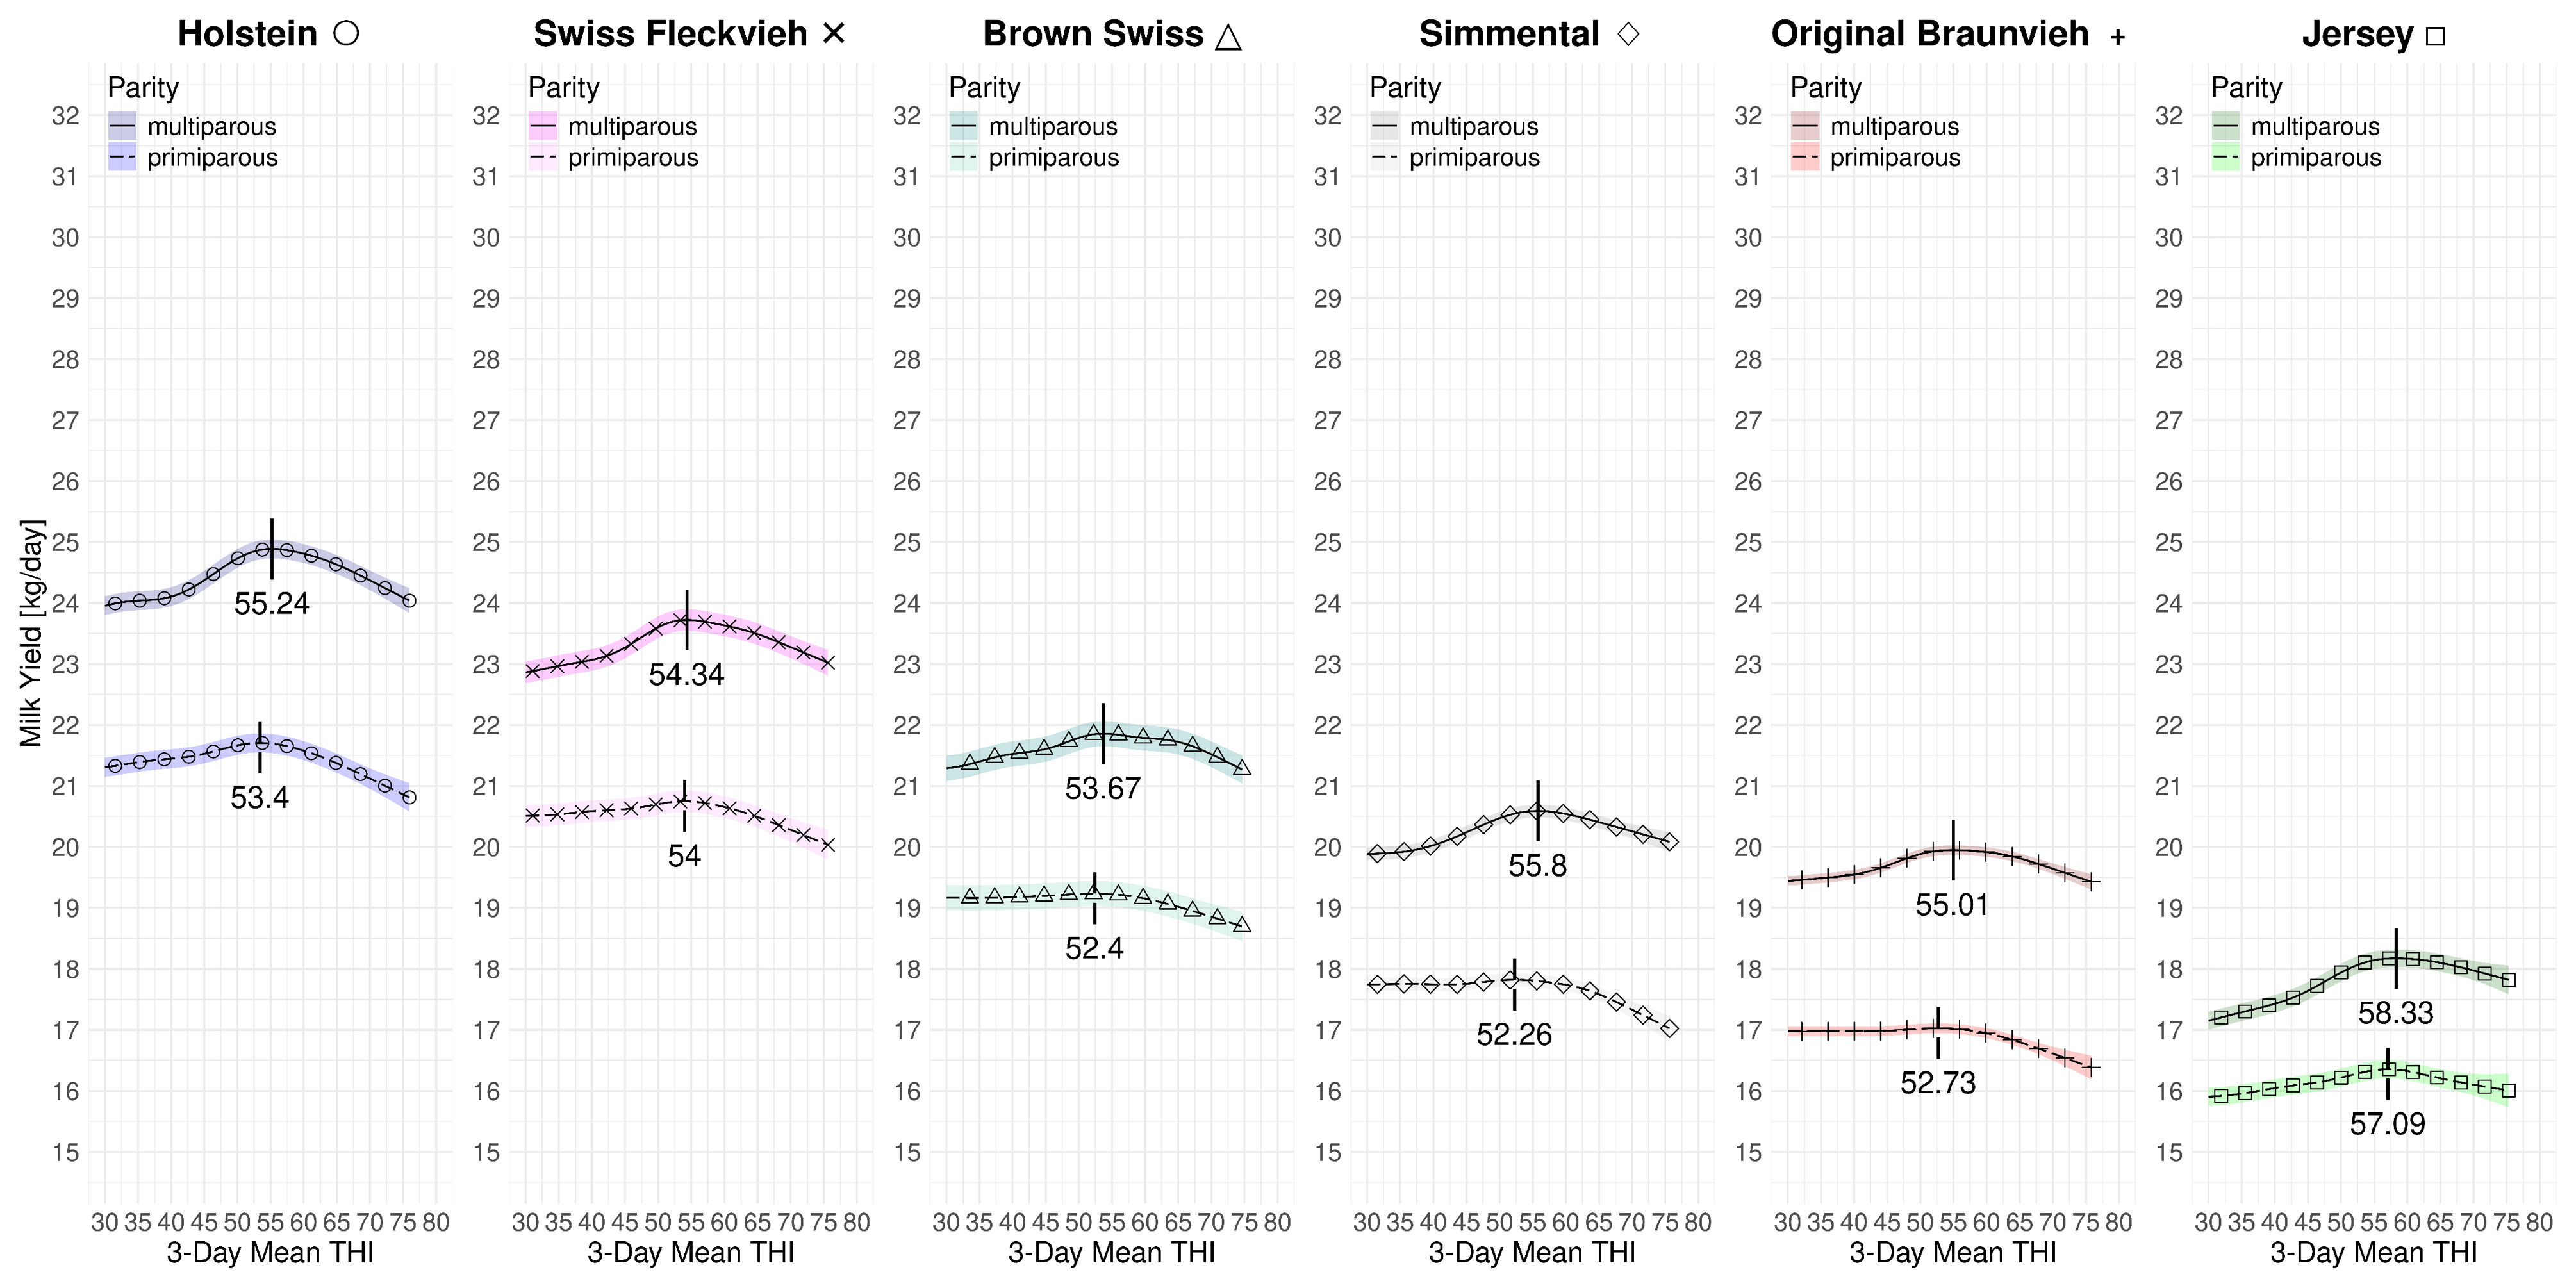
\includegraphics[width=0.85\paperheight]{thesis/figures/results/milk_yield_before_2010.png}
        \caption[]{3-day mean THI effect on milk yield for primi- and multiparous Swiss dairy cows at 2010 levels with data subsamples covering the full time period from 1982-2010.}
        \label{fig:results_milk_yield_before_2010}
    \end{figure}
    
    \begin{textblock*}{2cm}(20cm, \dimexpr\paperheight/2)
    \rotatebox{90}{\thepage}
    \end{textblock*}
\end{landscape}

\newpage
\begin{landscape}
    \thispagestyle{empty}
    \begin{figure}[ht]
        \centering
        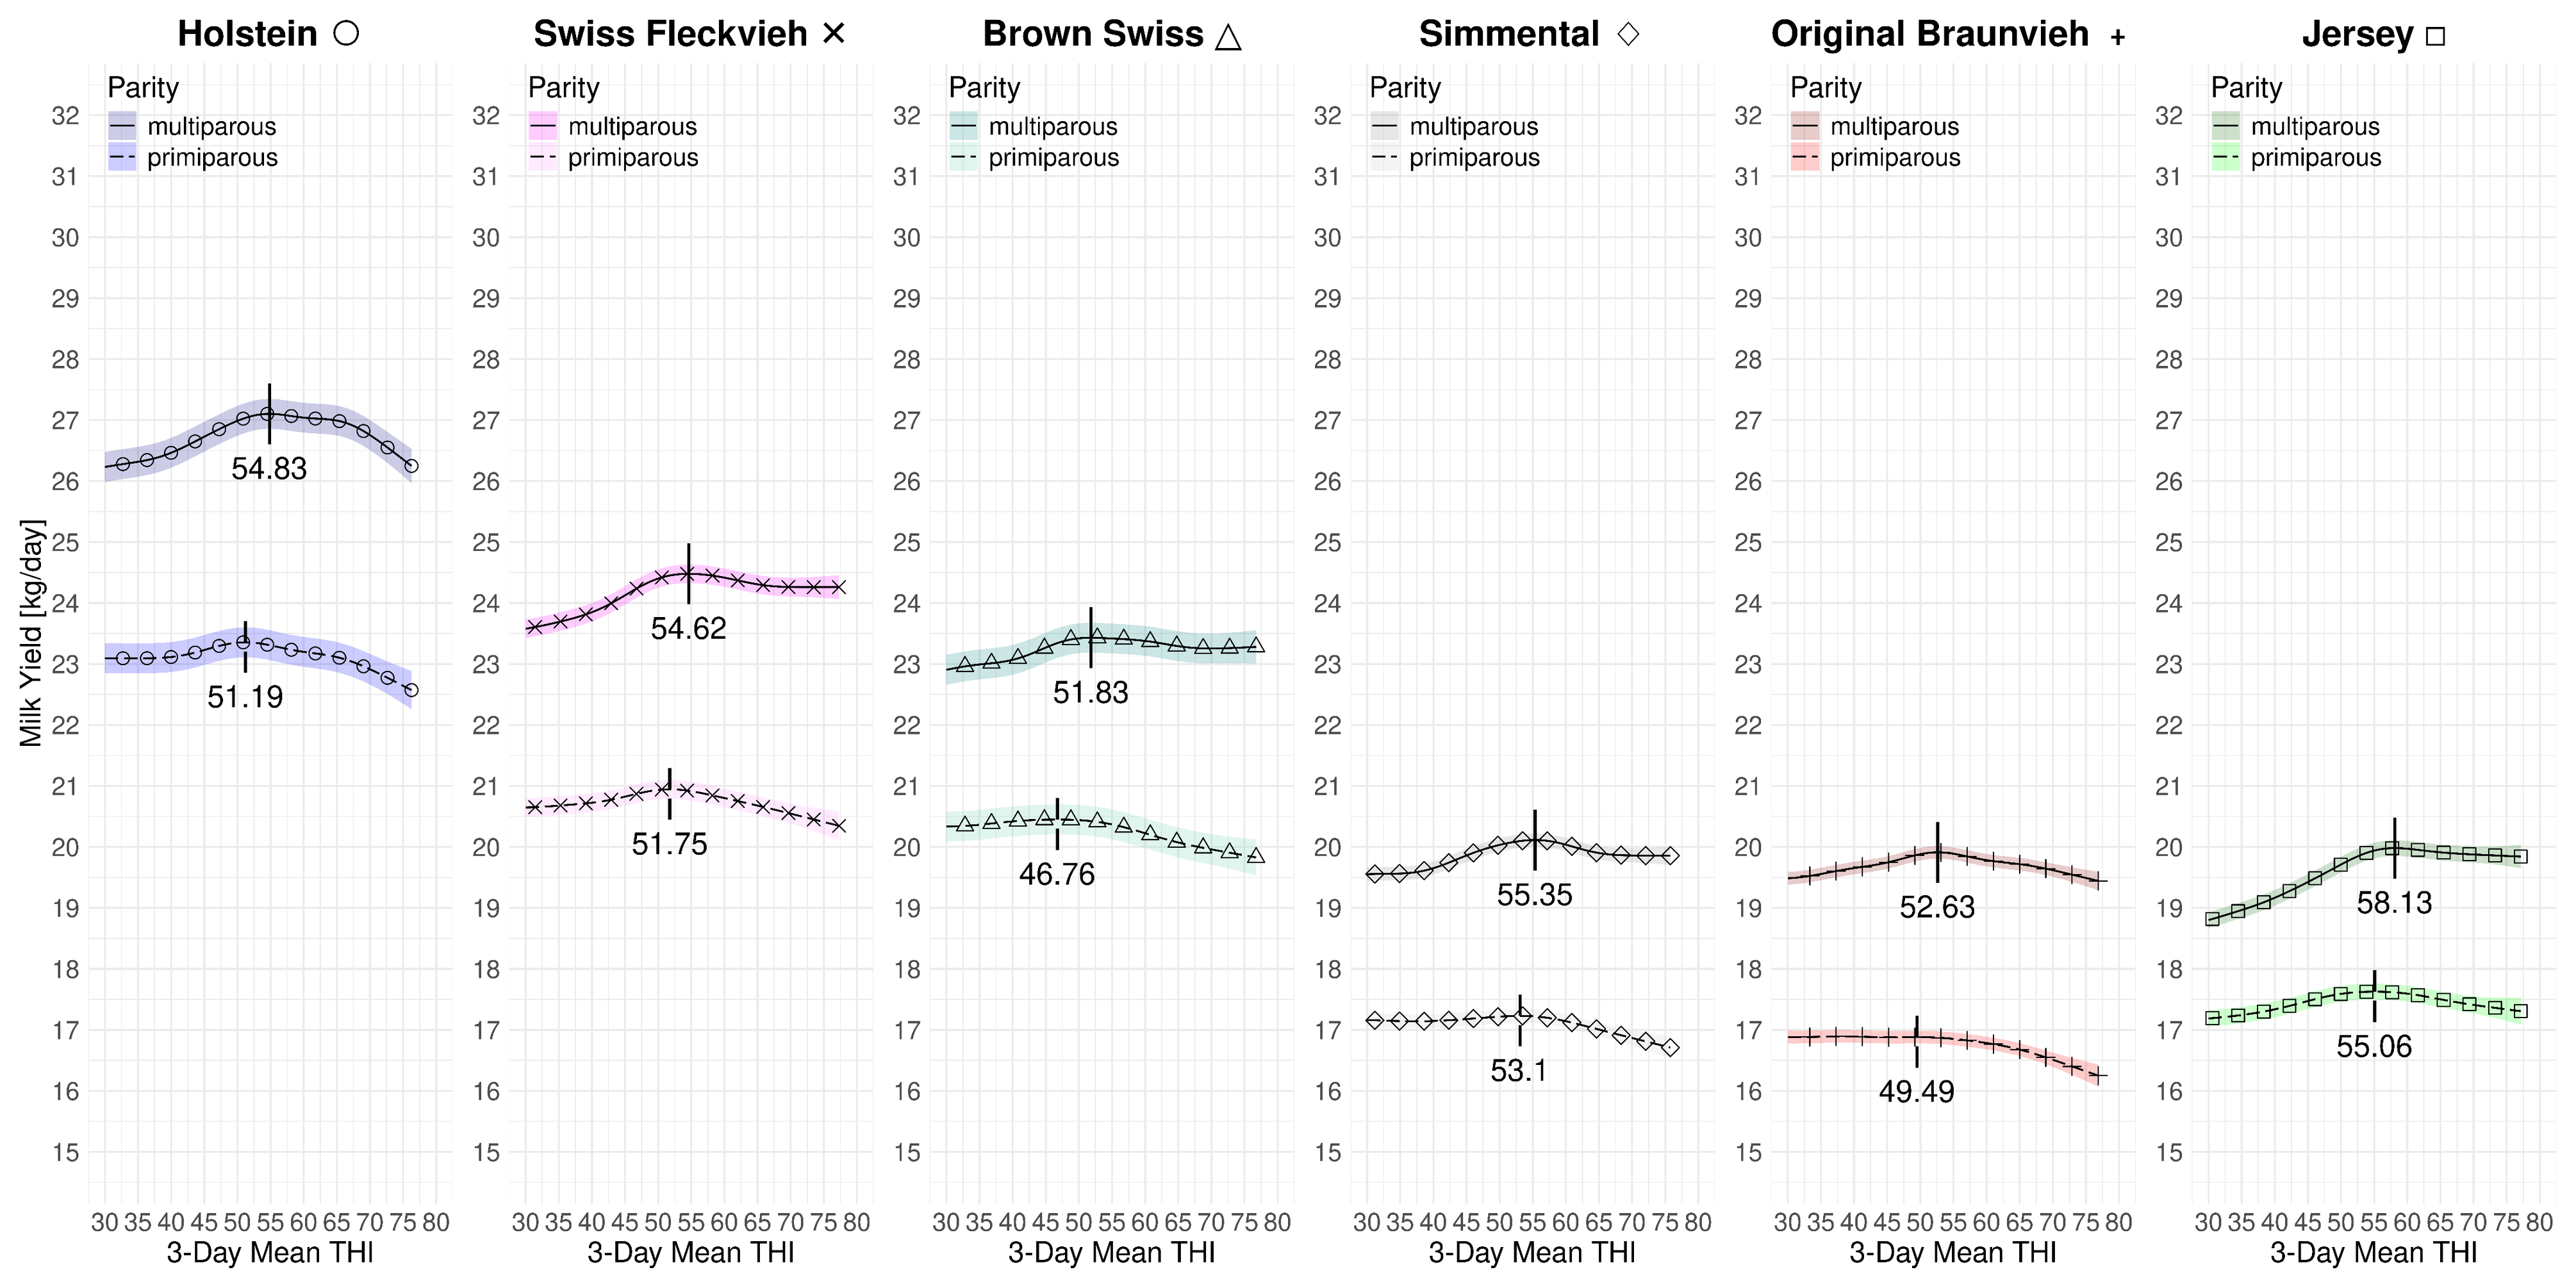
\includegraphics[width=0.85\paperheight]{thesis/figures/results/milk_yield_after_2010.png}
        \caption[]{3-day mean THI effect on milk yield for primi- and multiparous Swiss dairy cows at 2023 levels with data subsamples covering the full time period from 2011-2023}
        \label{fig:results_milk_yield_after_2010}
    \end{figure}
    
    \begin{textblock*}{2cm}(20cm, \dimexpr\paperheight/2)
    \rotatebox{90}{\thepage}
    \end{textblock*}
\end{landscape}


\newpage
\begin{landscape}
    \thispagestyle{empty}
    \section{ECM Yield}
    \begin{figure}[H]
        \centering
        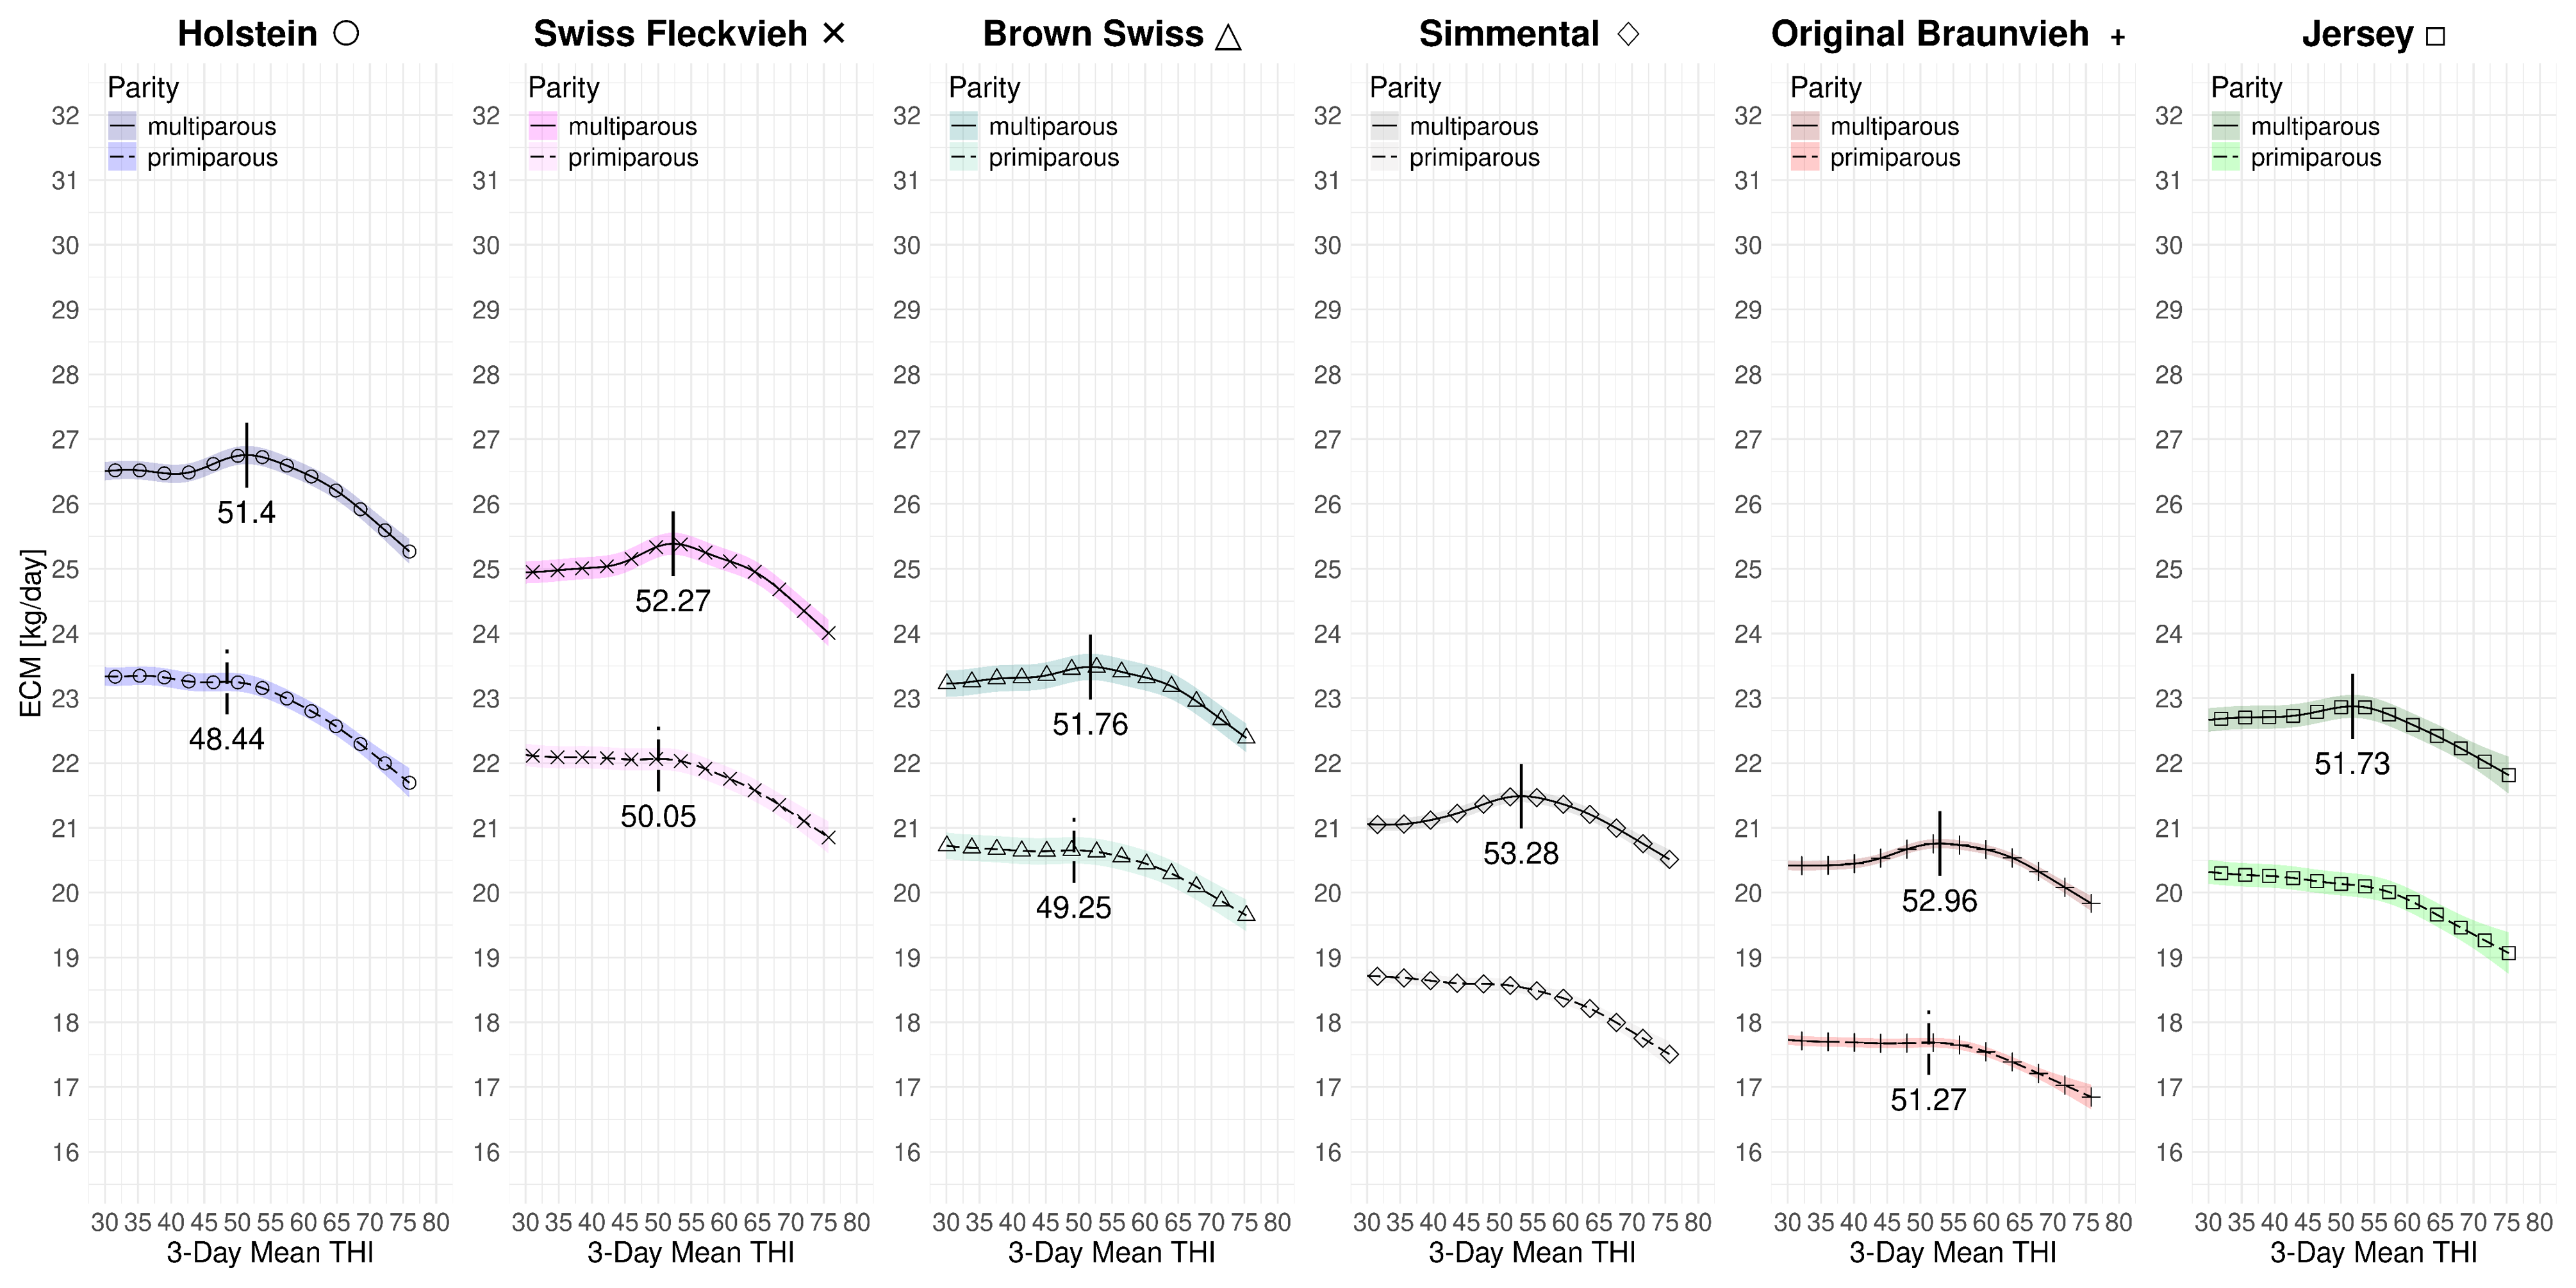
\includegraphics[width=0.85\paperheight]{thesis/figures/results/ecm_yield_before_2010.png}
        \caption[]{3-day mean THI effect on ECM yield for primi- and multiparous Swiss dairy cows at 2010 levels with data subsamples covering the full time period from 1982-2010.}
        \label{fig:results_ecm_yield_before_2010}
    \end{figure}
    
    \begin{textblock*}{2cm}(20cm, \dimexpr\paperheight/2)
    \rotatebox{90}{\thepage}
    \end{textblock*}
\end{landscape}
\newpage

\begin{landscape}
    \thispagestyle{empty}
    \begin{figure}[ht]
        \centering
        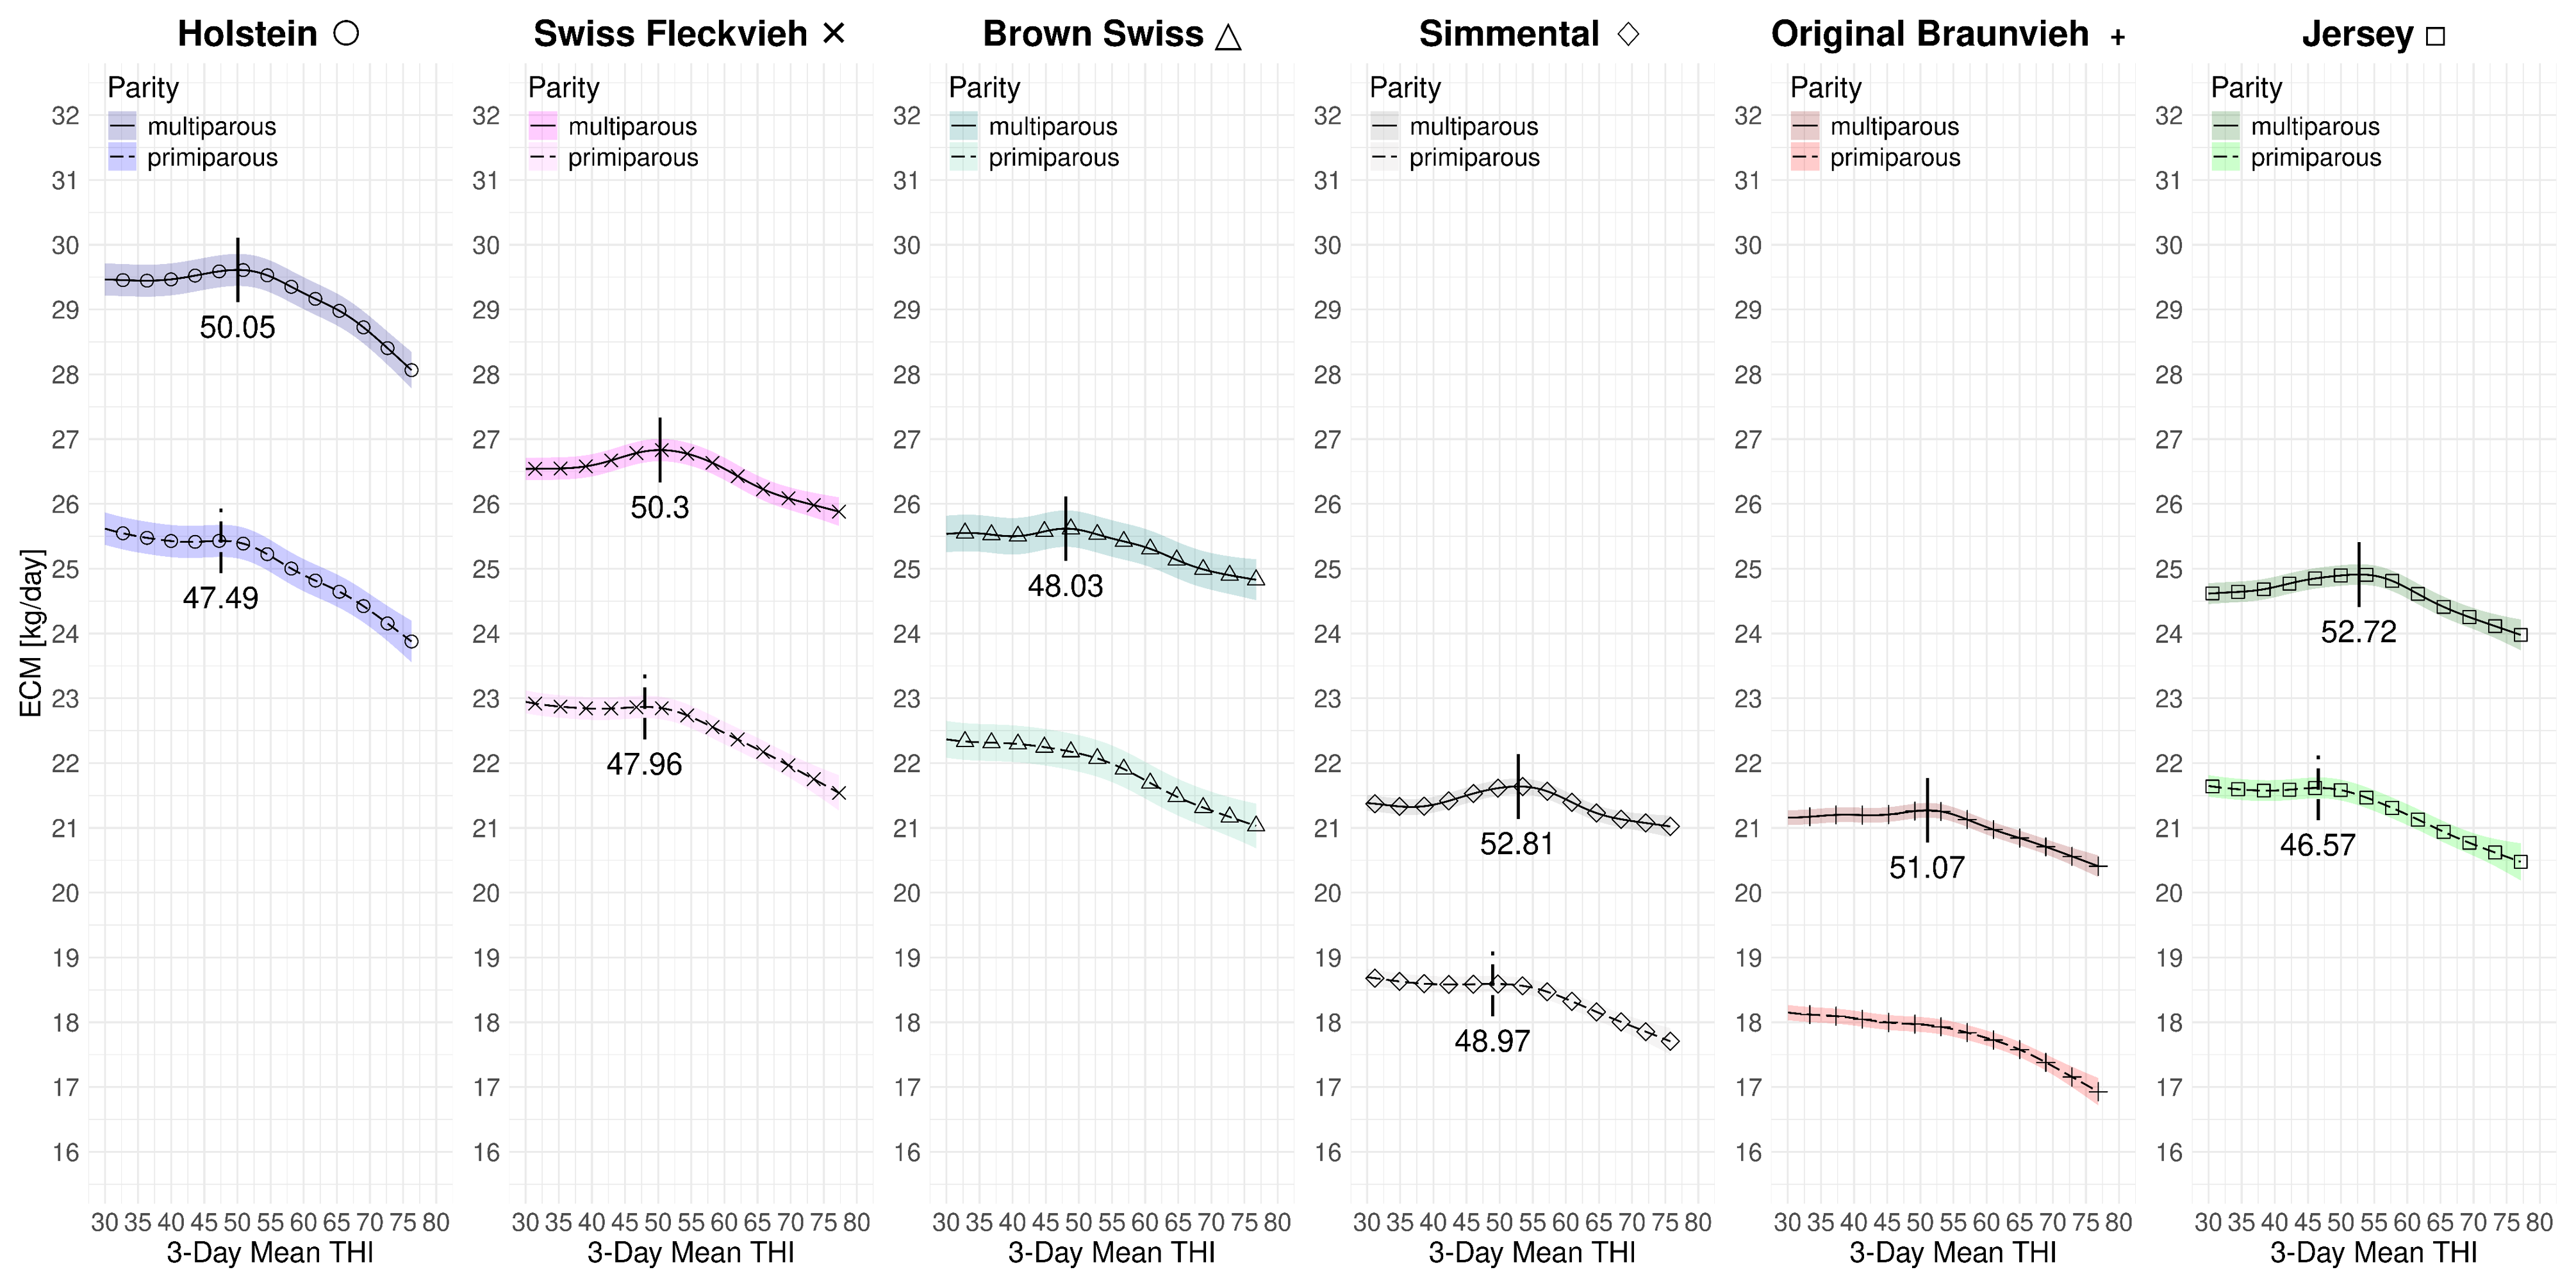
\includegraphics[width=0.85\paperheight]{thesis/figures/results/ecm_yield_after_2010.png}
        \caption[]{3-day mean THI effect on ECM yield for primi- and multiparous Swiss dairy cows at 2023 levels with data subsamples covering the full time period from 2011-2023.}
        \label{fig:results_ecm_yield_after_2010}
    \end{figure}
    
    \begin{textblock*}{2cm}(20cm, \dimexpr\paperheight/2)
    \rotatebox{90}{\thepage}
    \end{textblock*}
\end{landscape}


\chapter{Models}\label{appendix:models}

\newpage
\section{Holstein: Milk Yield}
\subsection{Full Period: 1985-2023}\label{model:ho_milk_full}
\paragraph{Model Summary} \quad \\

    \begin{table}[H]
    \centering
    \begin{tabular}{lrrrr}
    \textbf{A. parametric coefficients} & Estimate & Std. Error & t-value & p-value \\ 
       \hline
       \hline
  (Intercept) & 17.8235 & 0.6916 & 25.7716 & $<$ 0.0001 \\ 
  parityprimiparous & -3.4189 & 0.0129 & -264.1612 & $<$ 0.0001 \\ 
  year1986 & 0.3265 & 0.3478 & 0.9389 & 0.3478 \\ 
  year1987 & 0.1965 & 0.5377 & 0.3654 & 0.7148 \\ 
  year1988 & 0.0287 & 0.6610 & 0.0435 & 0.9653 \\ 
  year1989 & 0.5588 & 0.8363 & 0.6682 & 0.5040 \\ 
  year1990 & 0.8289 & 0.8270 & 1.0024 & 0.3162 \\ 
  year1991 & 0.9862 & 0.8085 & 1.2198 & 0.2226 \\ 
  year1992 & 1.3033 & 0.7913 & 1.6470 & 0.0996 \\ 
  year1993 & 1.3348 & 0.7892 & 1.6912 & 0.0908 \\ 
  year1994 & 1.2533 & 0.7838 & 1.5990 & 0.1098 \\ 
  year1995 & 1.5410 & 0.7860 & 1.9605 & 0.0499 \\ 
  year1996 & 1.7461 & 0.7837 & 2.2280 & 0.0259 \\ 
  year1997 & 2.2454 & 0.7879 & 2.8498 & 0.0044 \\ 
  year1998 & 2.8965 & 0.7939 & 3.6483 & 0.0003 \\ 
  year1999 & 2.8606 & 0.8275 & 3.4567 & 0.0005 \\ 
  year2000 & 3.0084 & 0.7605 & 3.9561 & 0.0001 \\ 
  year2001 & 3.1575 & 0.7423 & 4.2539 & $<$ 0.0001 \\ 
  year2002 & 3.5520 & 0.7379 & 4.8134 & $<$ 0.0001 \\ 
  year2003 & 3.9766 & 0.7361 & 5.4026 & $<$ 0.0001 \\ 
  year2004 & 4.3994 & 0.7339 & 5.9945 & $<$ 0.0001 \\ 
  year2005 & 4.8325 & 0.7330 & 6.5926 & $<$ 0.0001 \\ 
  year2006 & 4.9189 & 0.7324 & 6.7165 & $<$ 0.0001 \\ 
  year2007 & 4.7073 & 0.7264 & 6.4805 & $<$ 0.0001 \\ 
  year2008 & 5.0081 & 0.7264 & 6.8946 & $<$ 0.0001 \\ 
  year2009 & 5.4514 & 0.7225 & 7.5456 & $<$ 0.0001 \\ 
  year2010 & 6.0077 & 0.7211 & 8.3318 & $<$ 0.0001 \\ 
  year2011 & 6.2726 & 0.7234 & 8.6706 & $<$ 0.0001 \\ 
  year2012 & 6.2564 & 0.7278 & 8.5960 & $<$ 0.0001 \\ 
  year2013 & 5.9409 & 0.7442 & 7.9826 & $<$ 0.0001 \\ 
  year2014 & 6.5407 & 0.7493 & 8.7297 & $<$ 0.0001 \\ 
  year2015 & 6.9626 & 0.7412 & 9.3935 & $<$ 0.0001 \\ 
  year2016 & 7.3016 & 0.7404 & 9.8618 & $<$ 0.0001 \\ 
  year2017 & 7.5165 & 0.7399 & 10.1585 & $<$ 0.0001 \\ 
  year2018 & 8.0975 & 0.7432 & 10.8957 & $<$ 0.0001 \\ 
  year2019 & 8.2939 & 0.7587 & 10.9316 & $<$ 0.0001 \\ 
  year2020 & 8.7453 & 0.7749 & 11.2863 & $<$ 0.0001 \\ 
  year2021 & 9.2780 & 0.7623 & 12.1713 & $<$ 0.0001 \\ 
  year2022 & 9.4385 & 0.7518 & 12.5551 & $<$ 0.0001 \\ 
  year2023 & 9.9865 & 0.7507 & 13.3024 & $<$ 0.0001 \\ 
       \hline
    \textbf{B. smooth terms} & edf & Ref.df & F-value & p-value \\ 
    \hline
    \hline
  s(thi\_mean\_t0\_3d):paritymultiparous & 8.3629 & 8.3629 & 517.3513 & $<$ 0.0001 \\ 
  s(thi\_mean\_t0\_3d):parityprimiparous & 6.5585 & 6.5585 & 48.0496 & $<$ 0.0001 \\ 
  s(days\_in\_milk\_t):paritymultiparous & 14.5992 & 14.5992 & 120213.0040 & $<$ 0.0001 \\ 
  s(days\_in\_milk\_t):parityprimiparous & 14.0843 & 14.0843 & 14232.8232 & $<$ 0.0001 \\ 
       \hline
    \end{tabular}
    \caption[]{Holstein: Milk Yield - 1985-2023 - GAMM model summary without random effect terms.}
    \end{table}

\newpage
\begin{table}[H]
\centering
\begin{tabular}
{l | r | r | r | r}
\textbf{Smooth Term Fixed Effect} & Est. & SE & z & p\\
\hline
\hline
s(thi\_mean\_t0\_3d):multiFx1 & 0.4424 & 0.1070 & 4.14 & <1e-04\\
s(thi\_mean\_t0\_3d):primiFx1 & 0.3466 & 0.1162 & 2.98 & 0.0028\\
s(days\_in\_milk\_):multiFx1 & 5.0429 & 0.5387 & 9.36 & <1e-20\\
s(days\_in\_milk\_):primiFx1 & 4.8631 & 0.6608 & 7.36 & <1e-12\\
\hline
\textbf{Variance Component} & Estimated $\sigma$ & & & \\
\hline
\hline
$\sigma_\alpha$ & 3.1230 & &  & \\
$\sigma_\iota$ & 1.0079 & & & \\
$\sigma_\phi$ & 3.1247 & & & \\
s(thi\_mean\_t0\_3d):multi & 2.3664 & & & \\
s(days\_in\_milk\_):primi & 9.0384 & & & \\
s(days\_in\_milk\_):multi & 10.9130 & & & \\
s(thi\_mean\_t0\_3d):primi & 1.2902 & & & \\
Residual & 3.7902 & & & \\
\end{tabular}
\caption[]{Holstein: Milk Yield - 1985-2023 - Mixed Model Summary - Smooth Terms and Random Effects.}
\end{table}

\paragraph{Model Diagnostics} \quad \\
\begin{figure}[H]
    \centering
    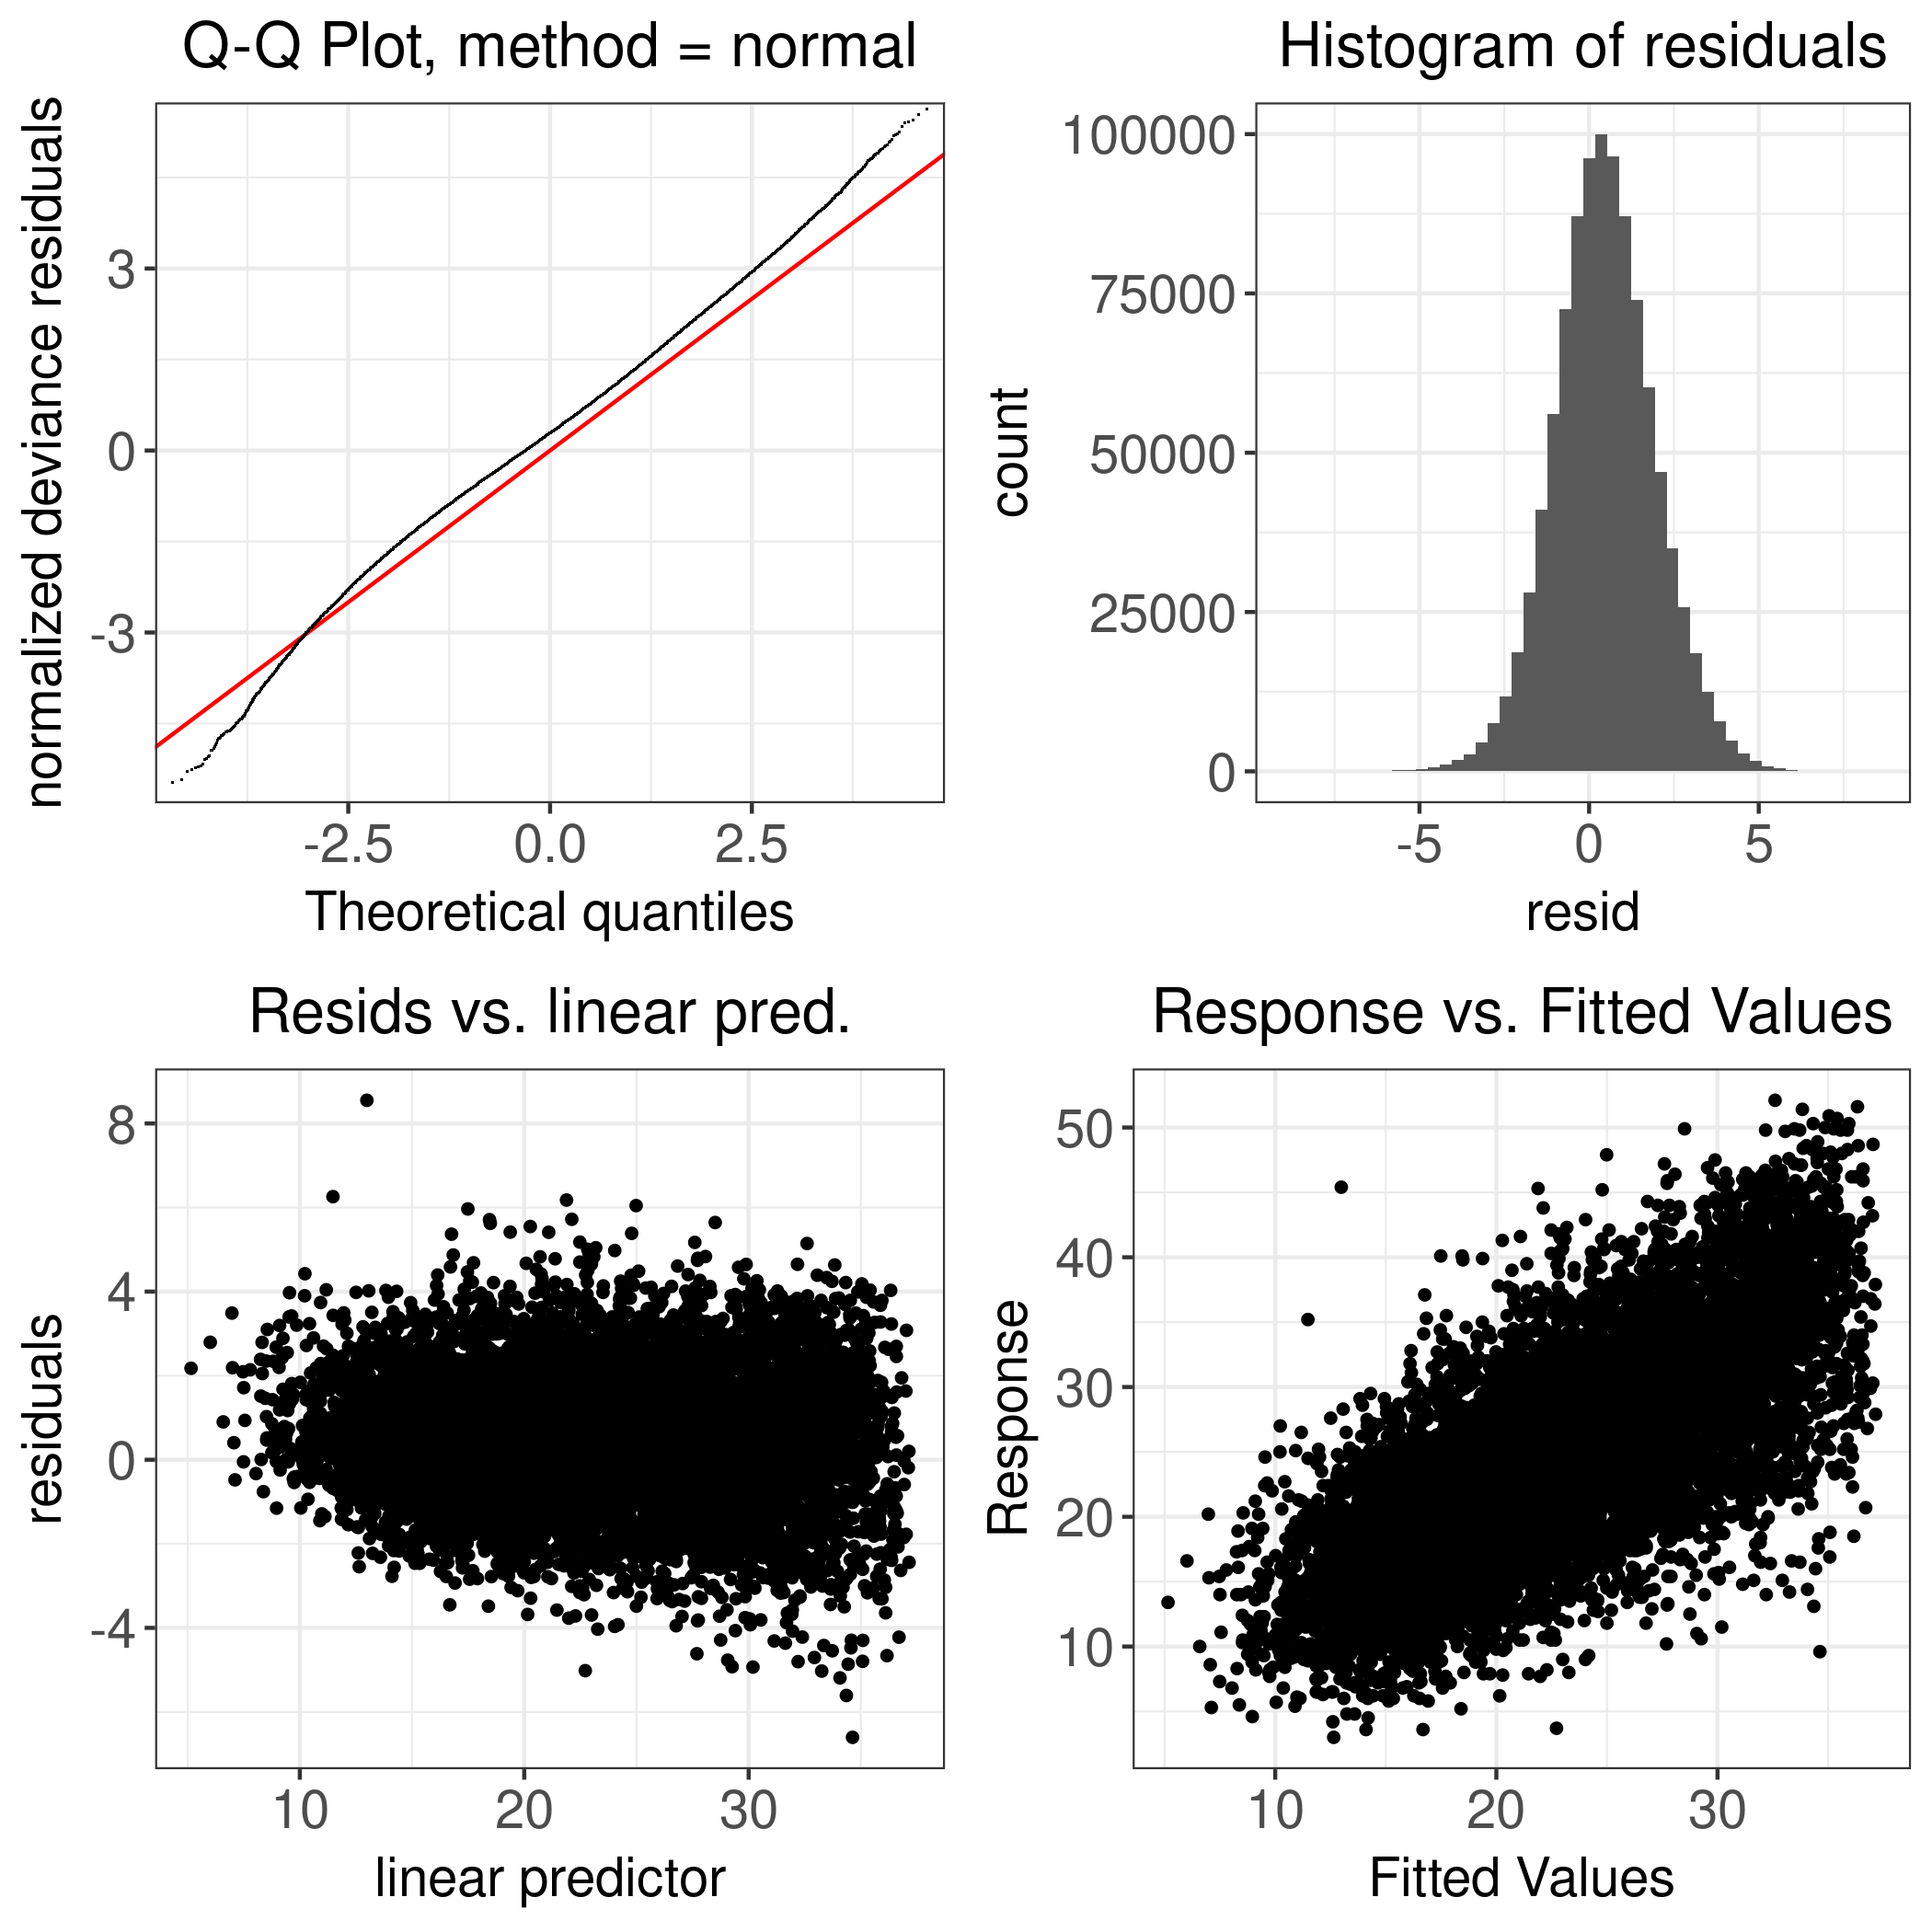
\includegraphics[width=0.6\textwidth]{thesis/figures/models/milk/full/ho_milk_full/ho_milk_full_diagnostics.png}
    \caption[]{Holstein: Milk Yield - 1985-2023 - Diagnostic Plot}
\end{figure}

\newpage
\paragraph{THI Effect and Lactation Curve} \quad \\
\begin{figure}[H]
    \centering
    \begin{subfigure}[b]{0.45\textwidth}
        \centering
        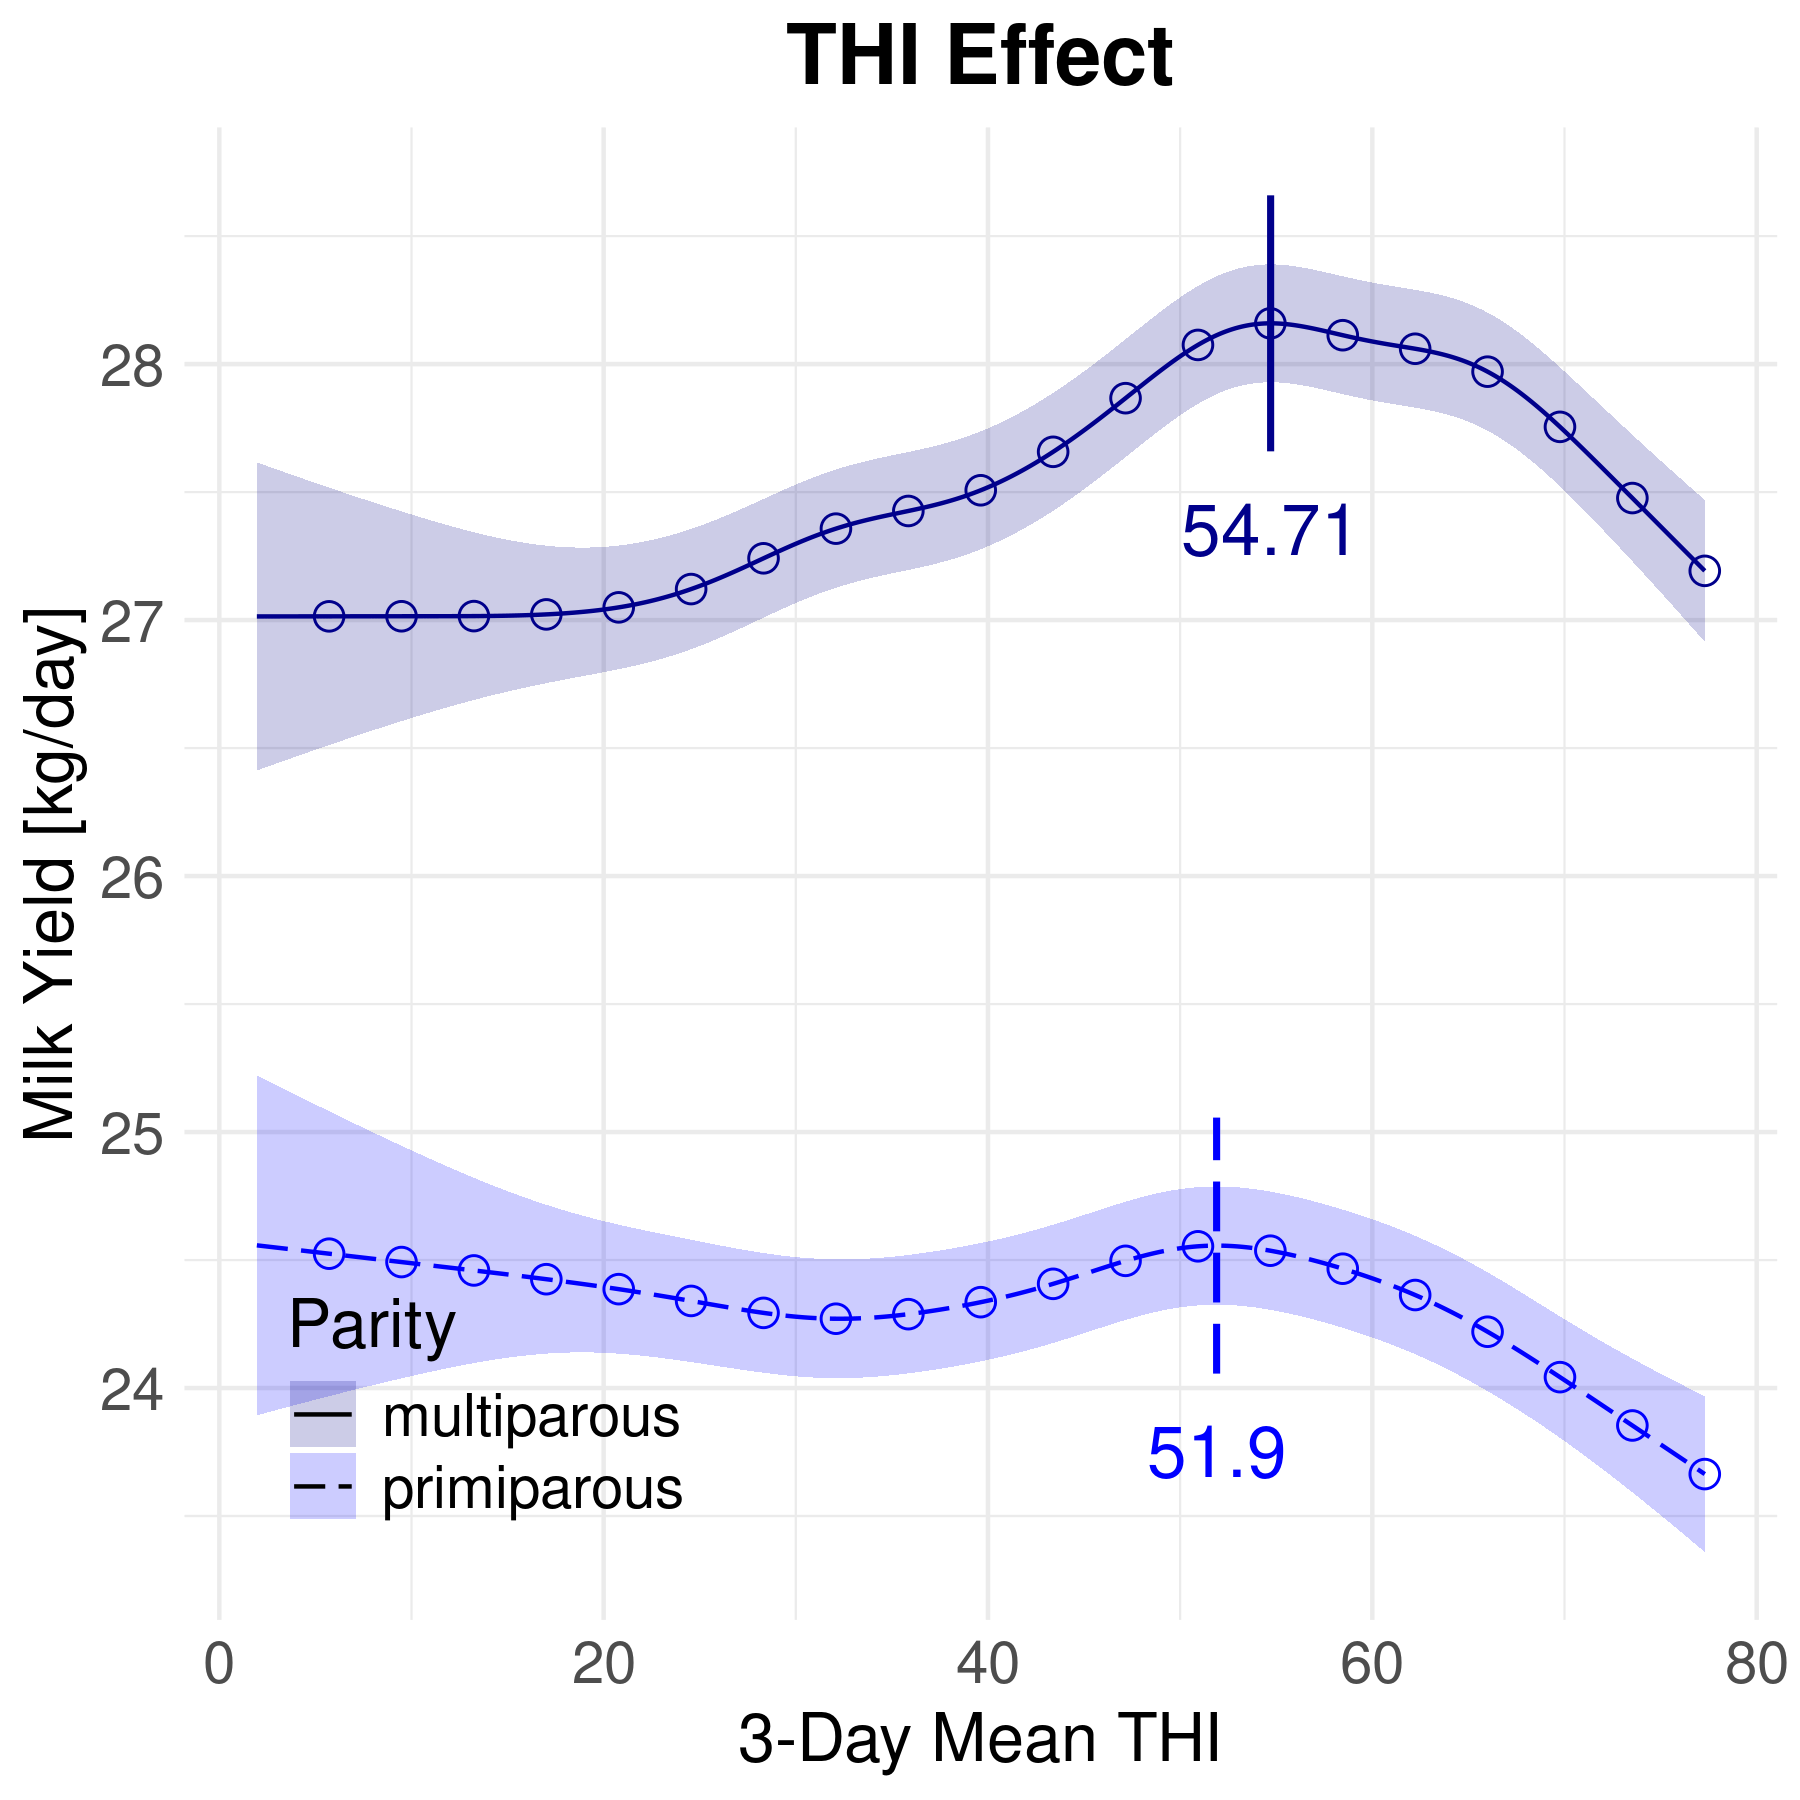
\includegraphics[width=\textwidth]{thesis/figures/models/milk/full/ho_milk_full/ho_milk_full_marginal_thi_milk_combined.png}
    \end{subfigure}
    \hspace{0.05\textwidth} % Optional space between the figures
    \begin{subfigure}[b]{0.45\textwidth}
        \centering
        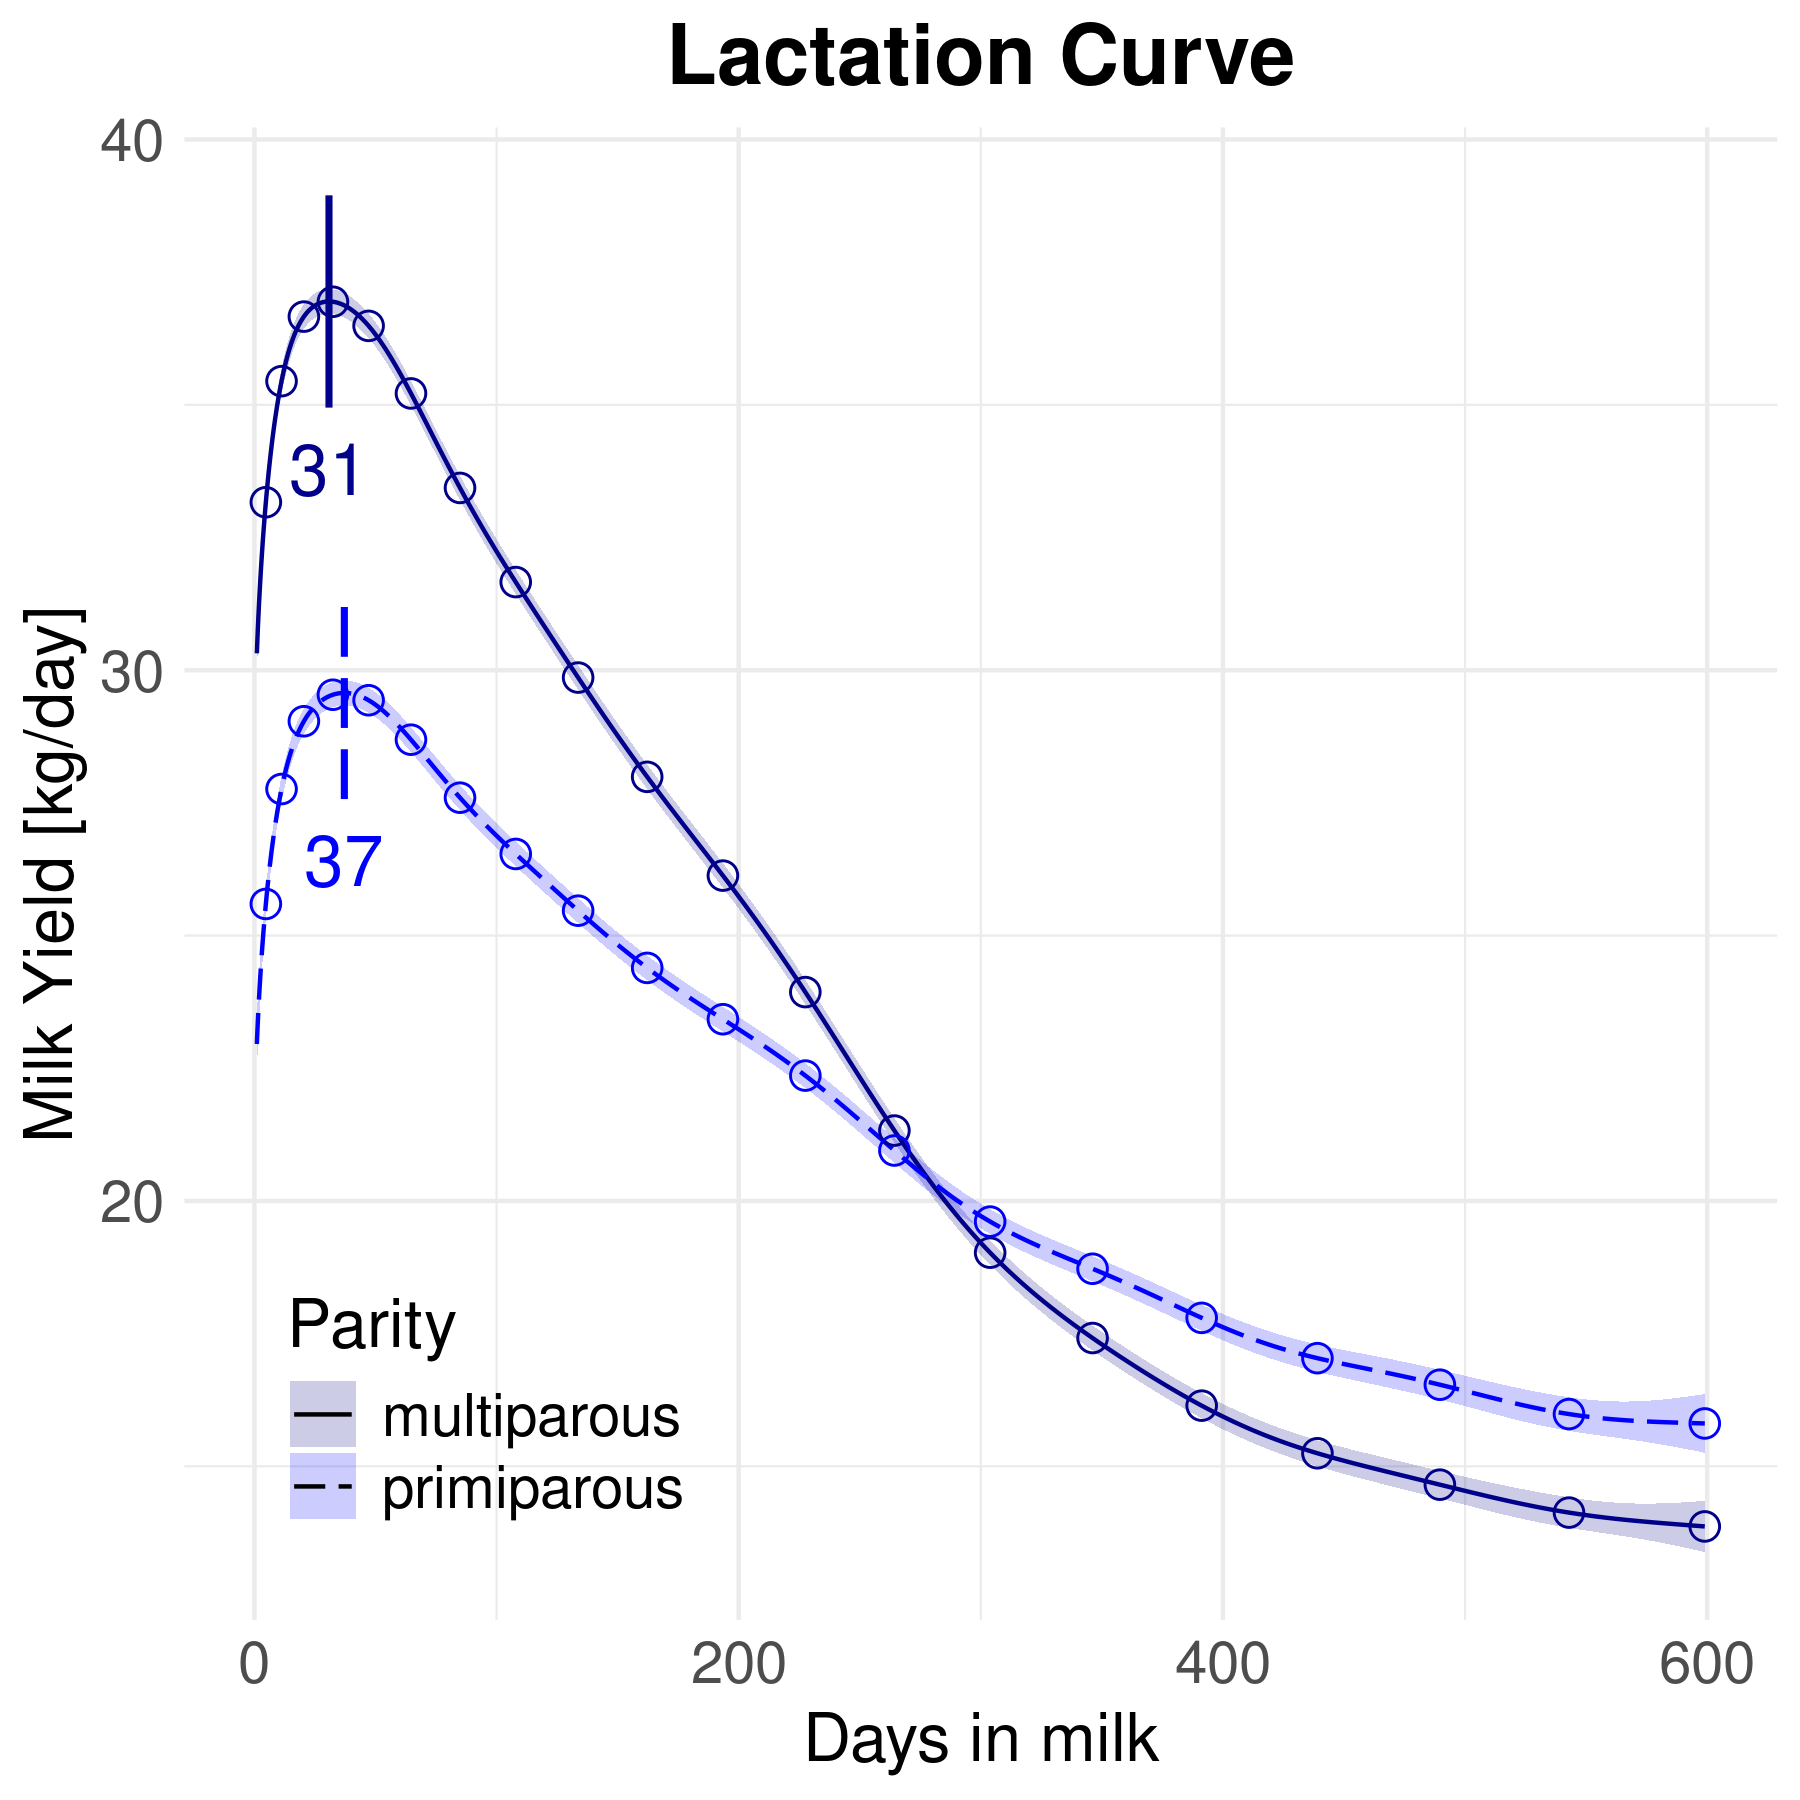
\includegraphics[width=\textwidth]{thesis/figures/models/milk/full/ho_milk_full/ho_milk_full_marginal_dim_milk_combined.png}
    \end{subfigure}
    \begin{subfigure}[b]{0.45\textwidth}
        \centering
        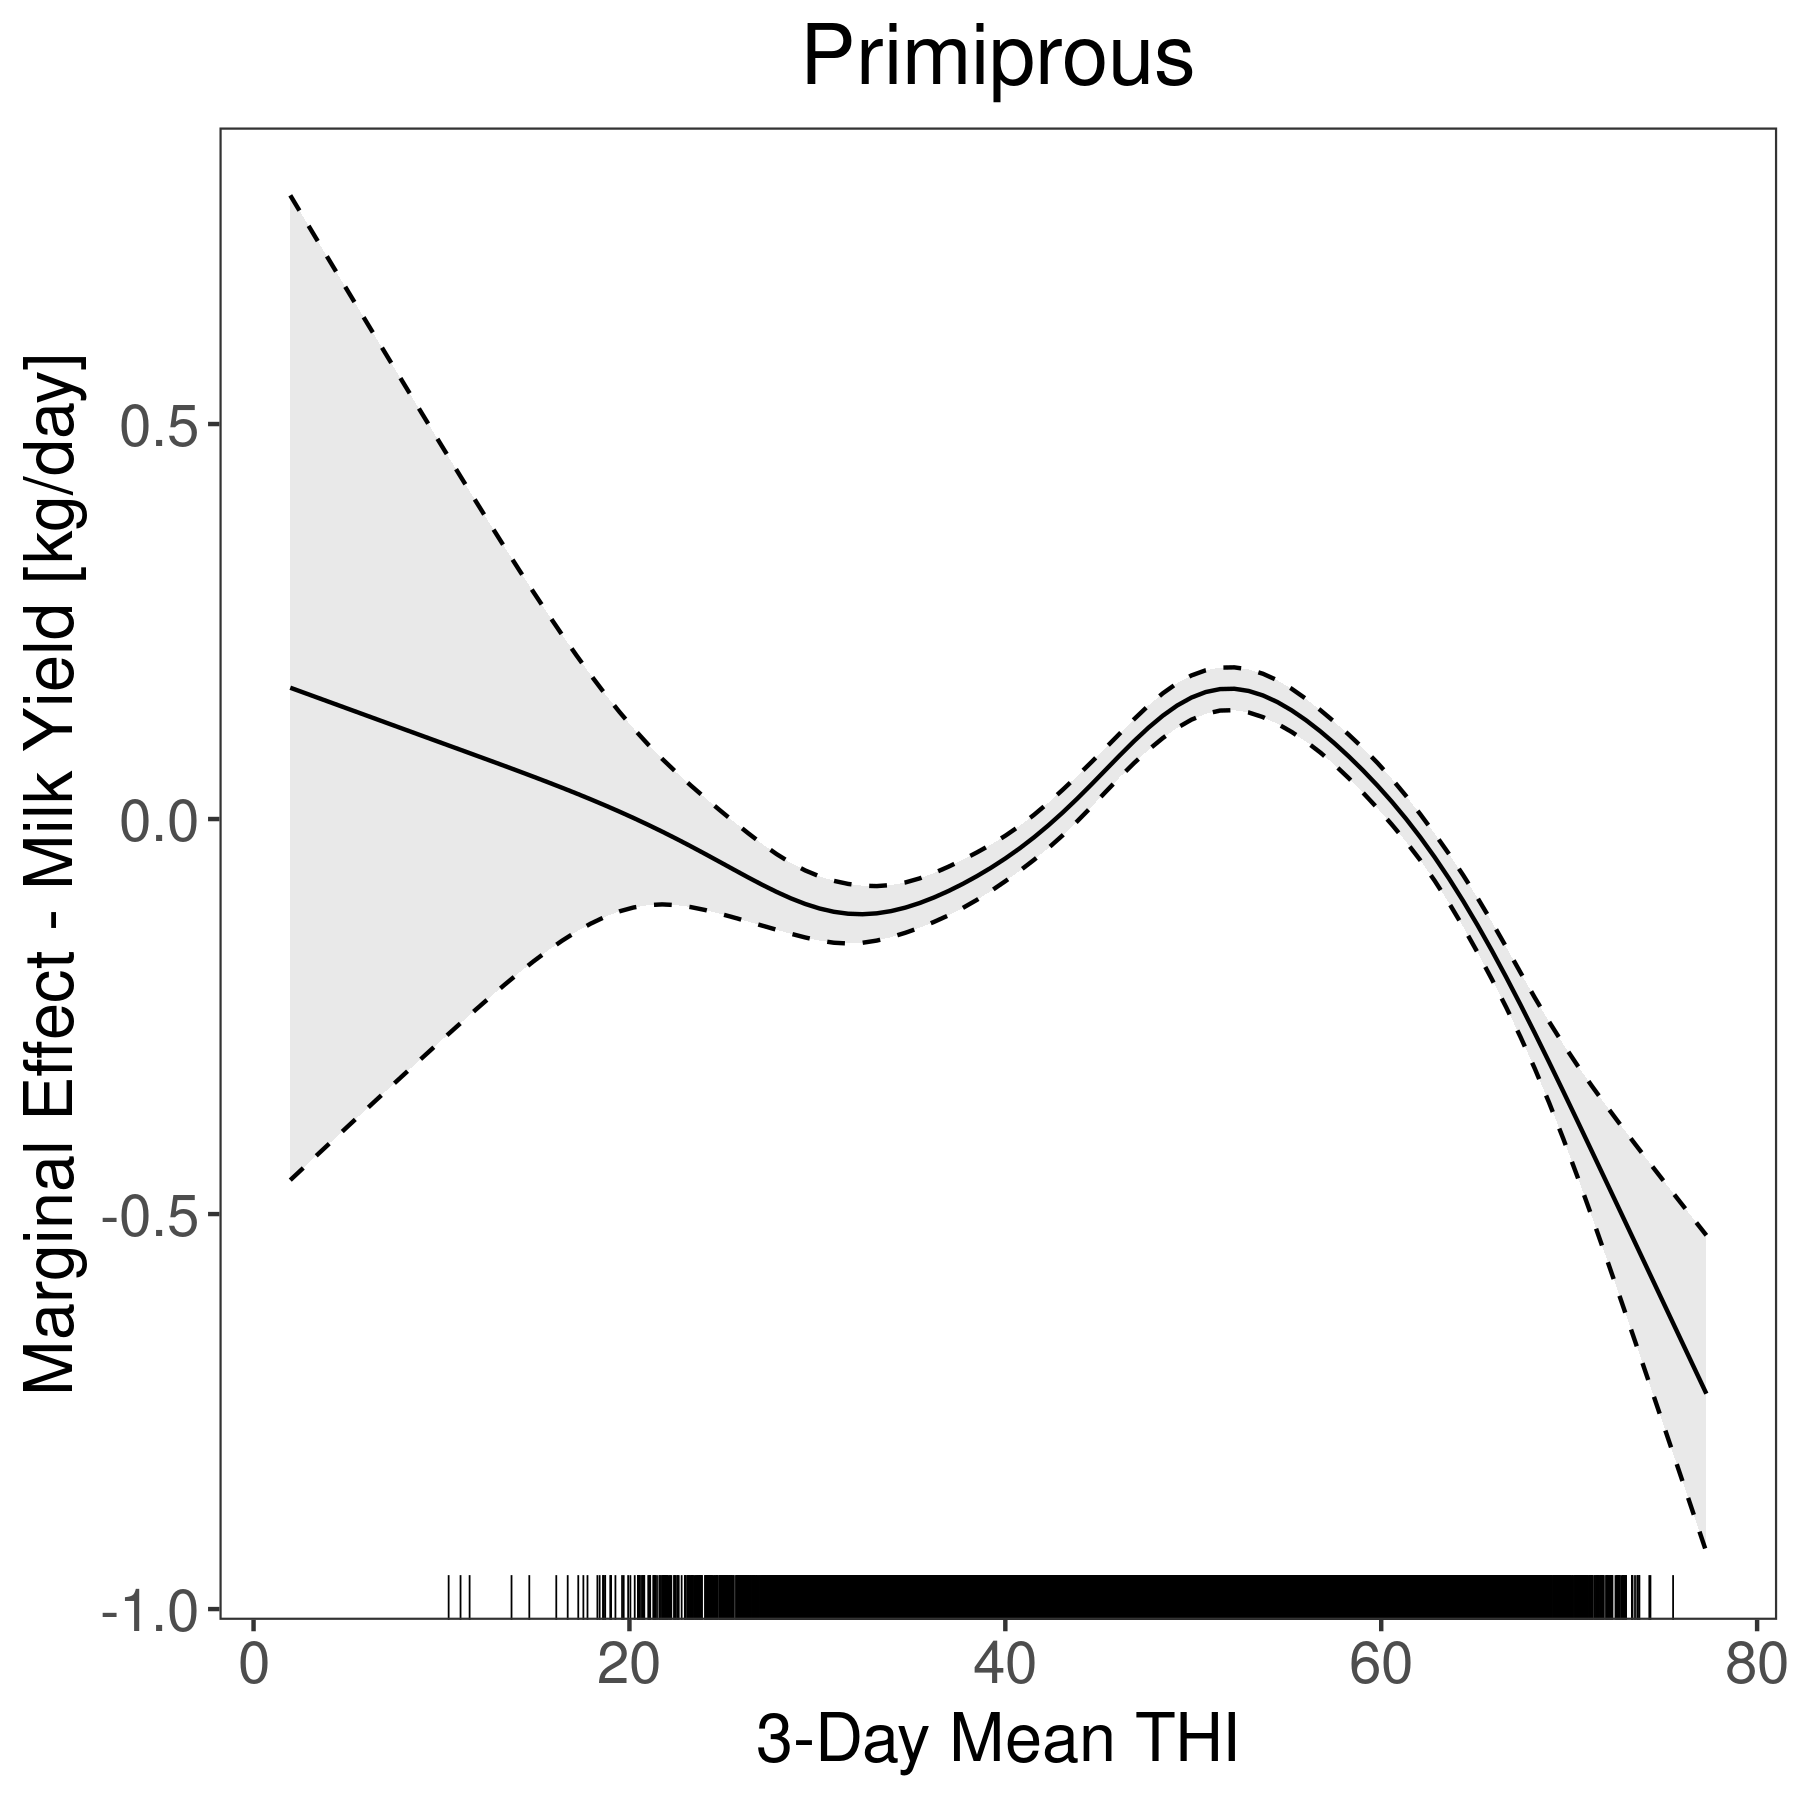
\includegraphics[width=\textwidth]{thesis/figures/models/milk/full/ho_milk_full/ho_milk_full_marginal_thi_milk_primi.png}
    \end{subfigure}
    \hspace{0.05\textwidth} % Optional space between the figures
    \begin{subfigure}[b]{0.45\textwidth}
        \centering
        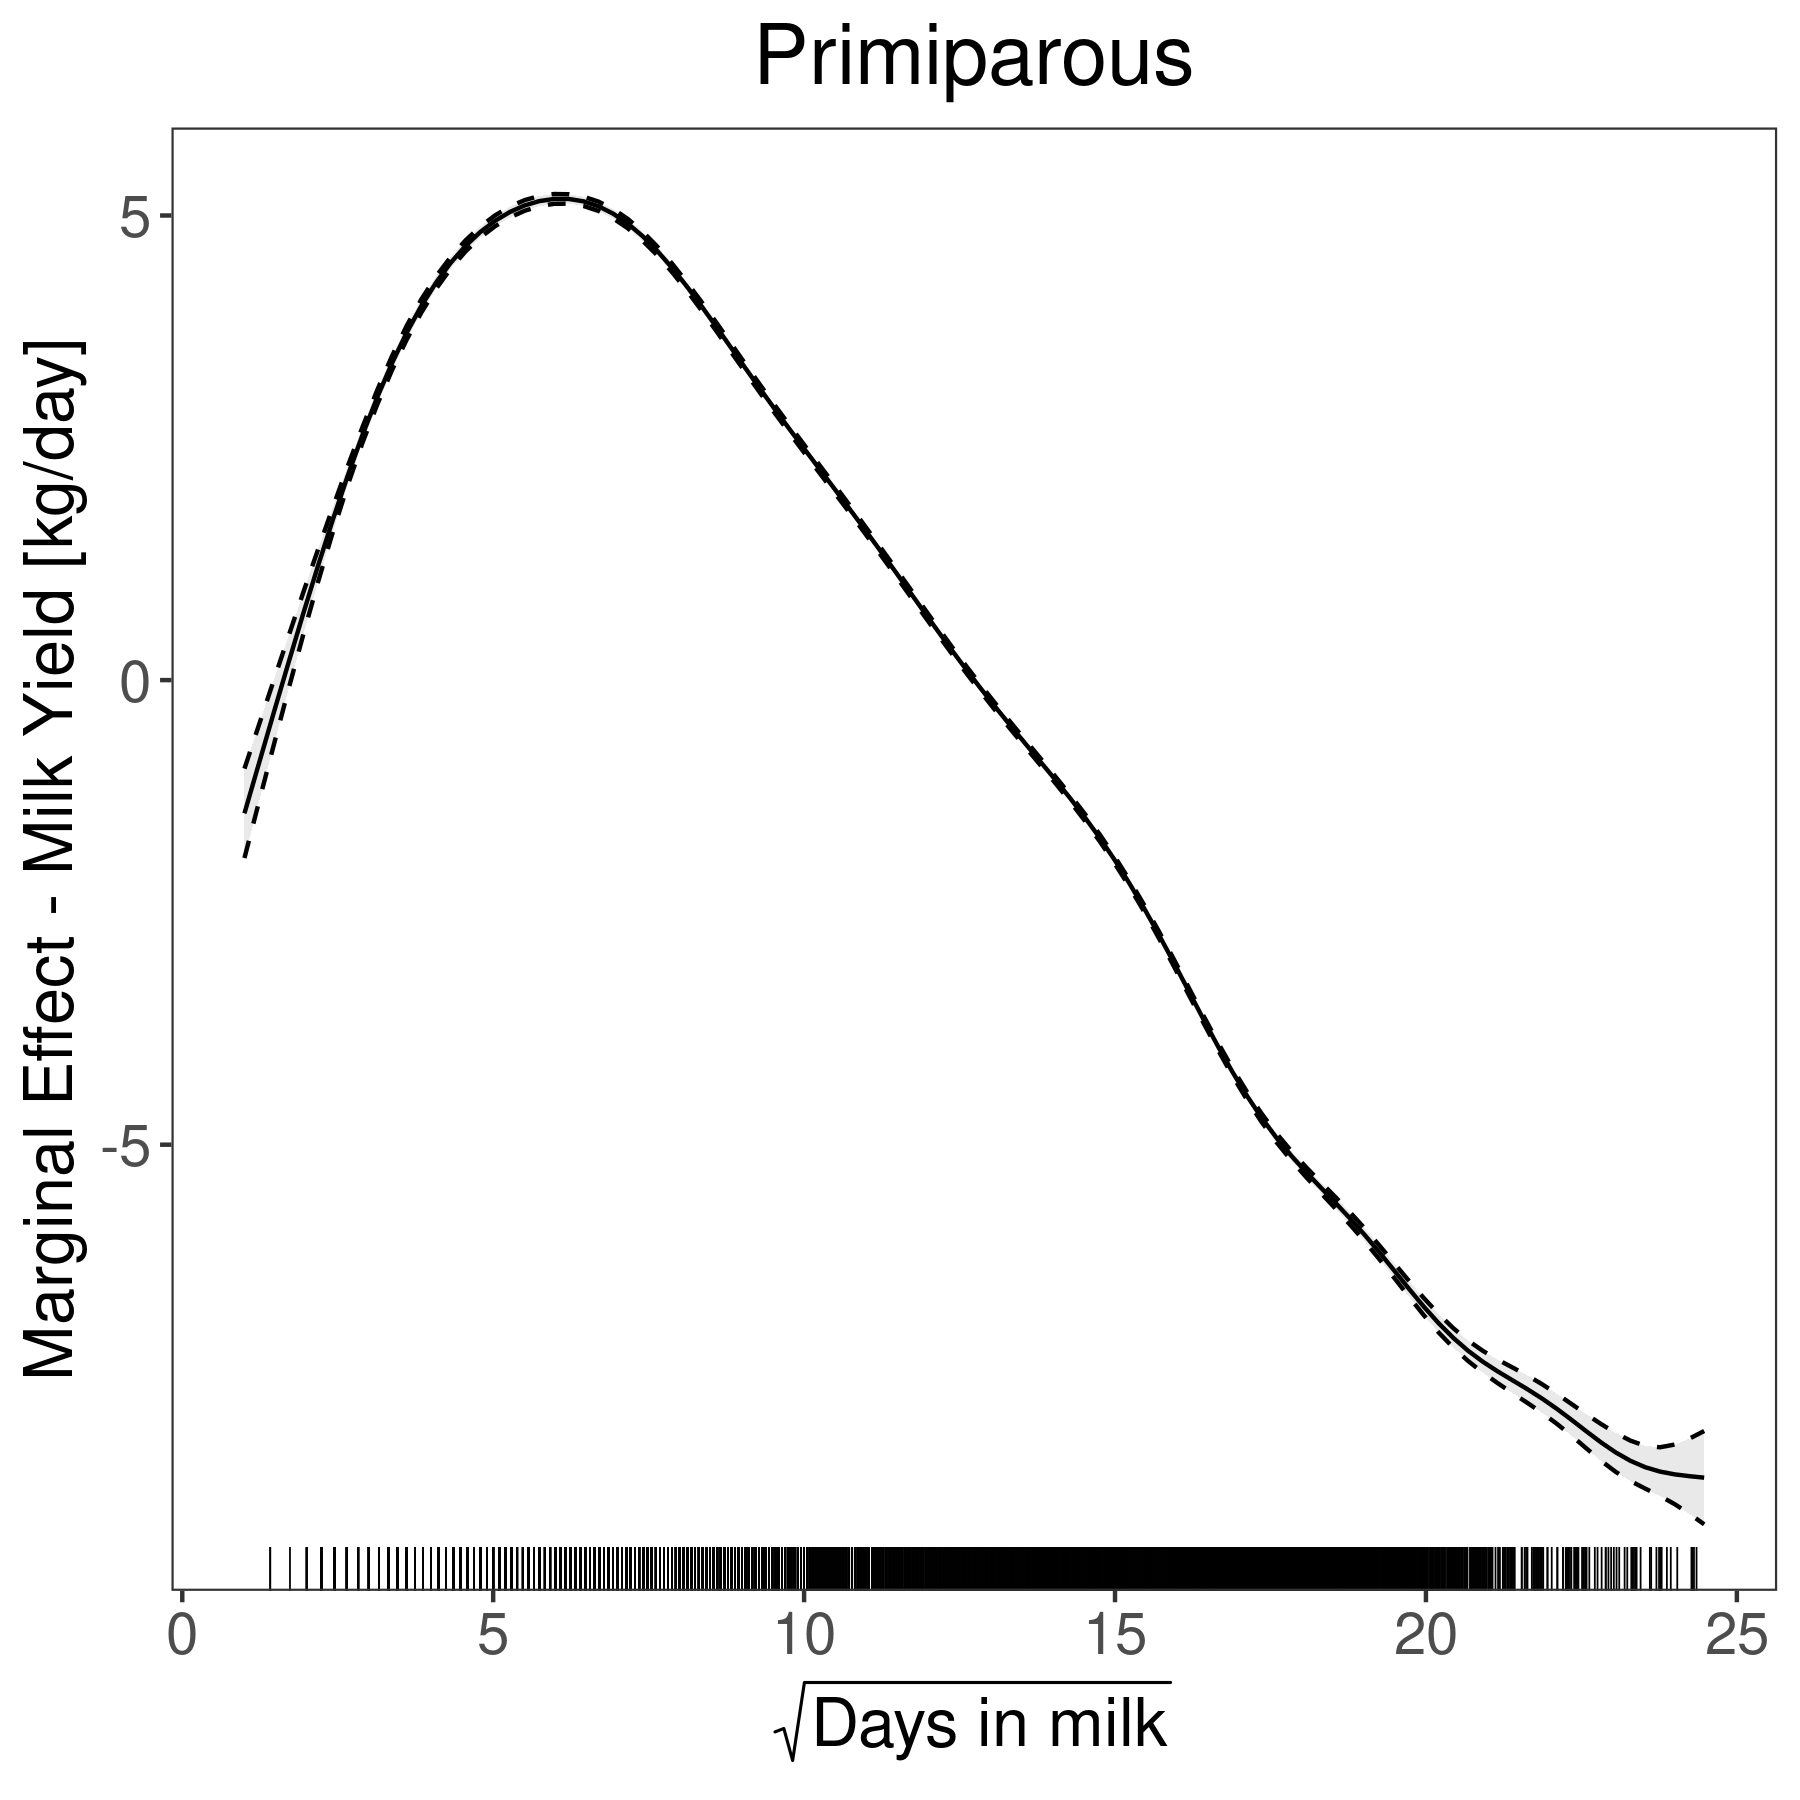
\includegraphics[width=\textwidth]{thesis/figures/models/milk/full/ho_milk_full/ho_milk_full_marginal_dim_milk_primi.png}
    \end{subfigure}
    \begin{subfigure}[b]{0.45\textwidth}
        \centering
        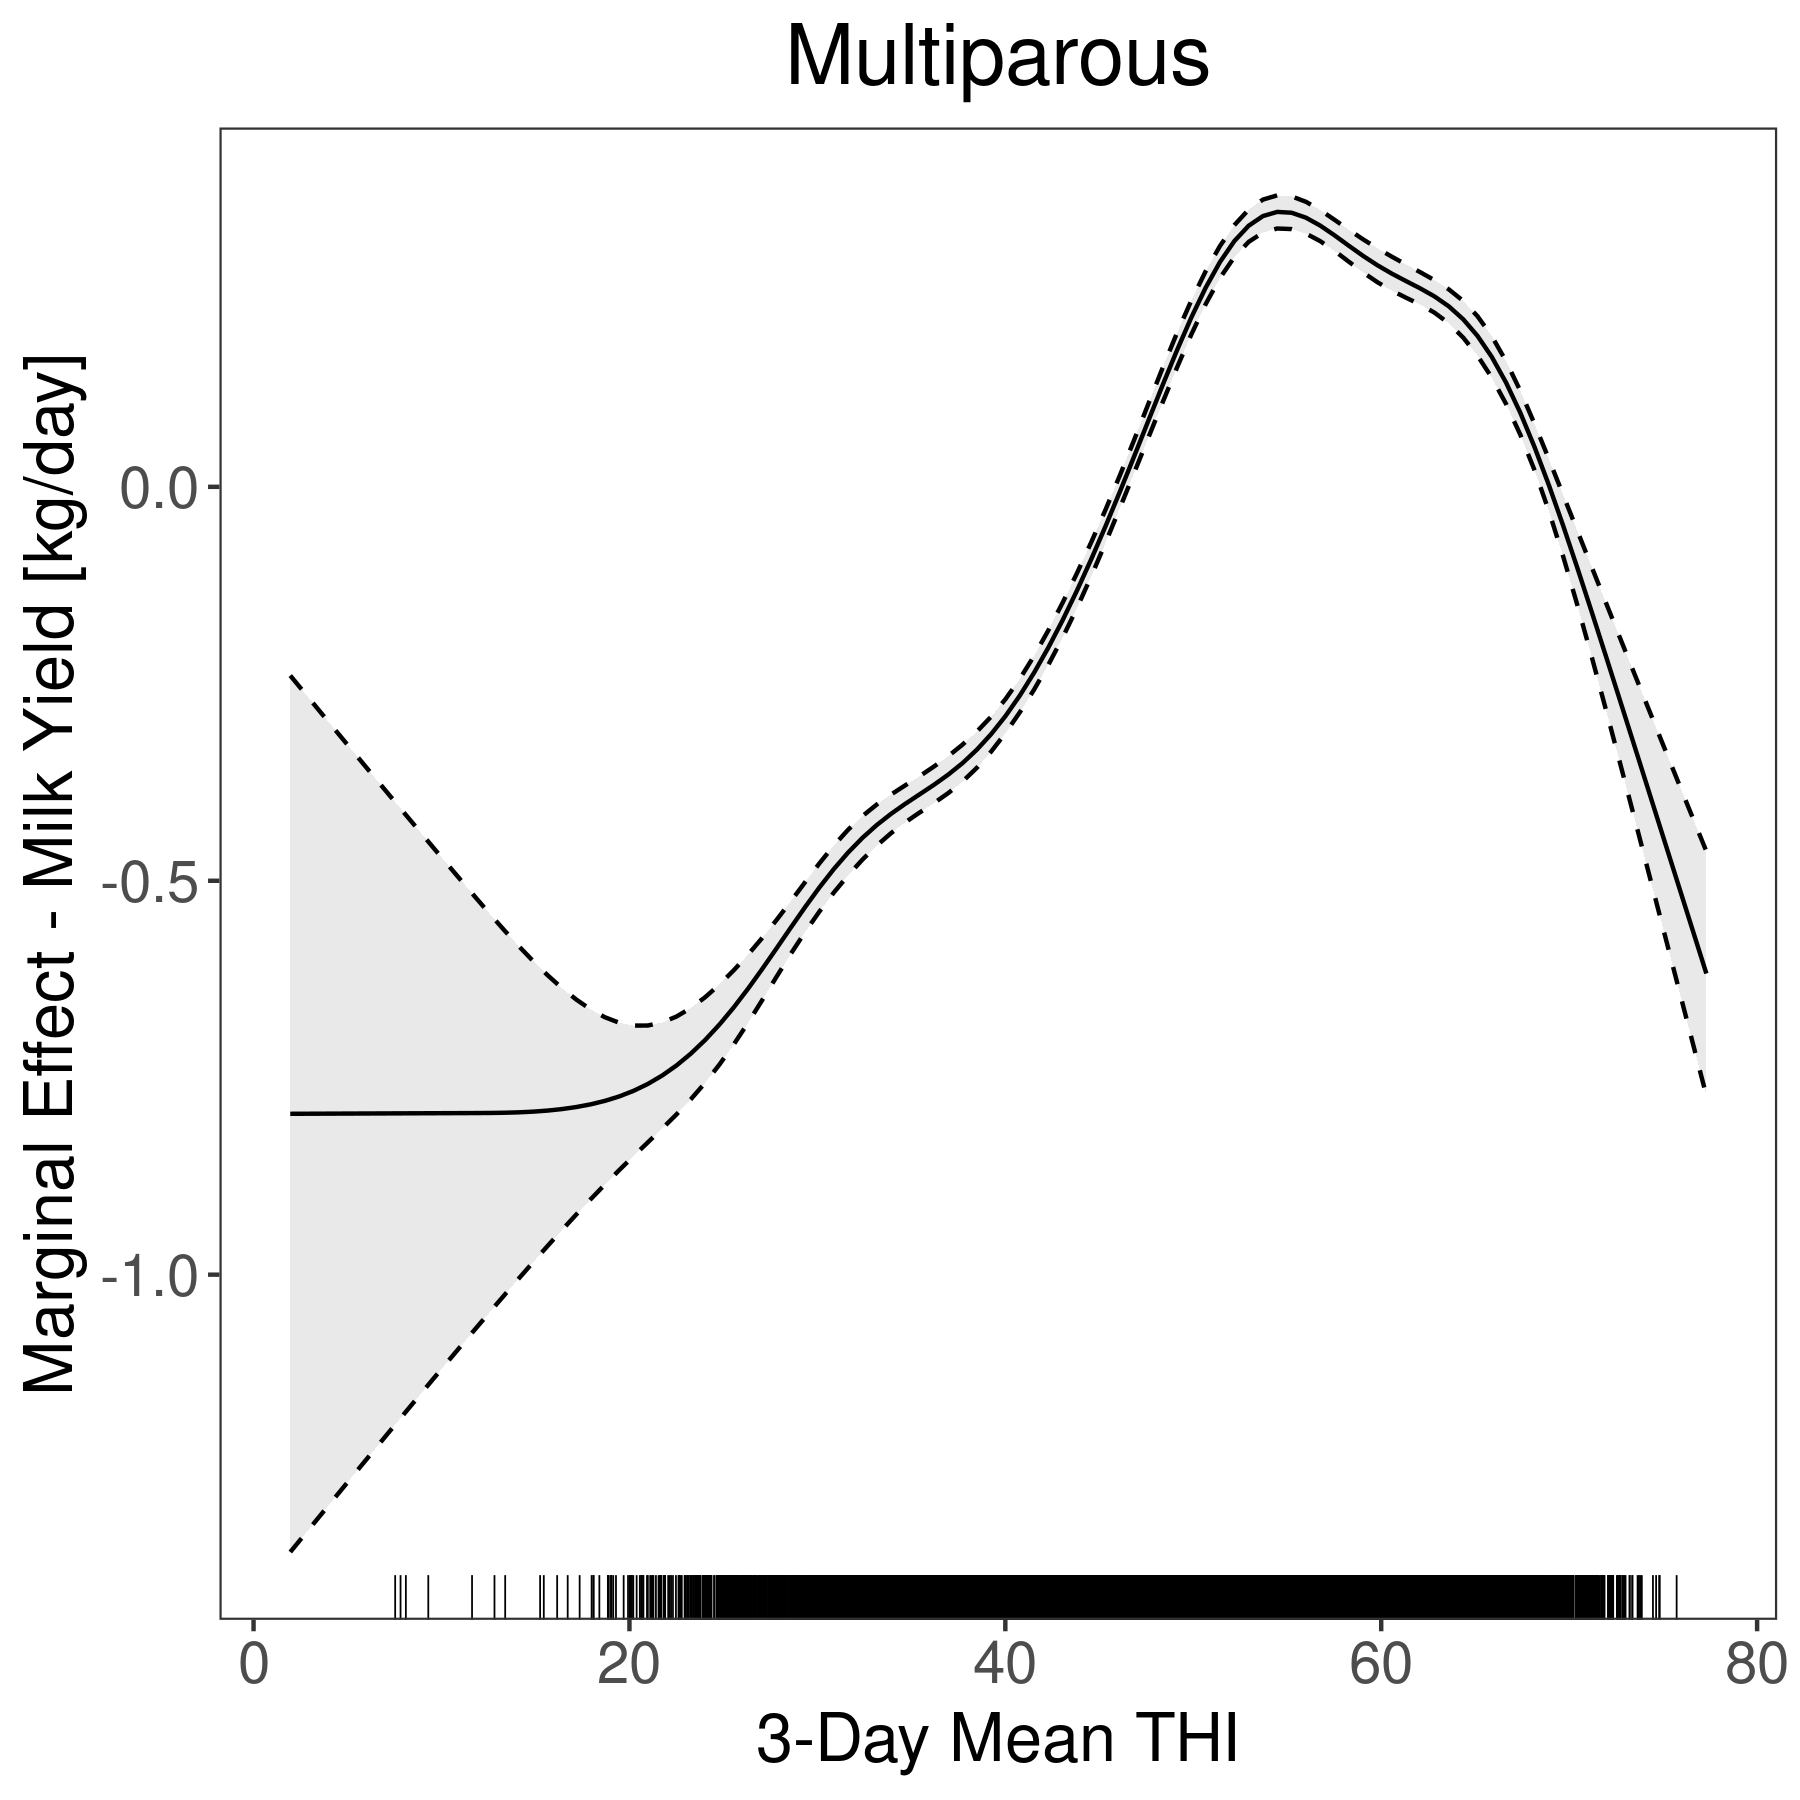
\includegraphics[width=\textwidth]{thesis/figures/models/milk/full/ho_milk_full/ho_milk_full_marginal_thi_milk_multi.png}
    \end{subfigure}
    \hspace{0.05\textwidth} % Optional space between the figures
    \begin{subfigure}[b]{0.45\textwidth}
        \centering
        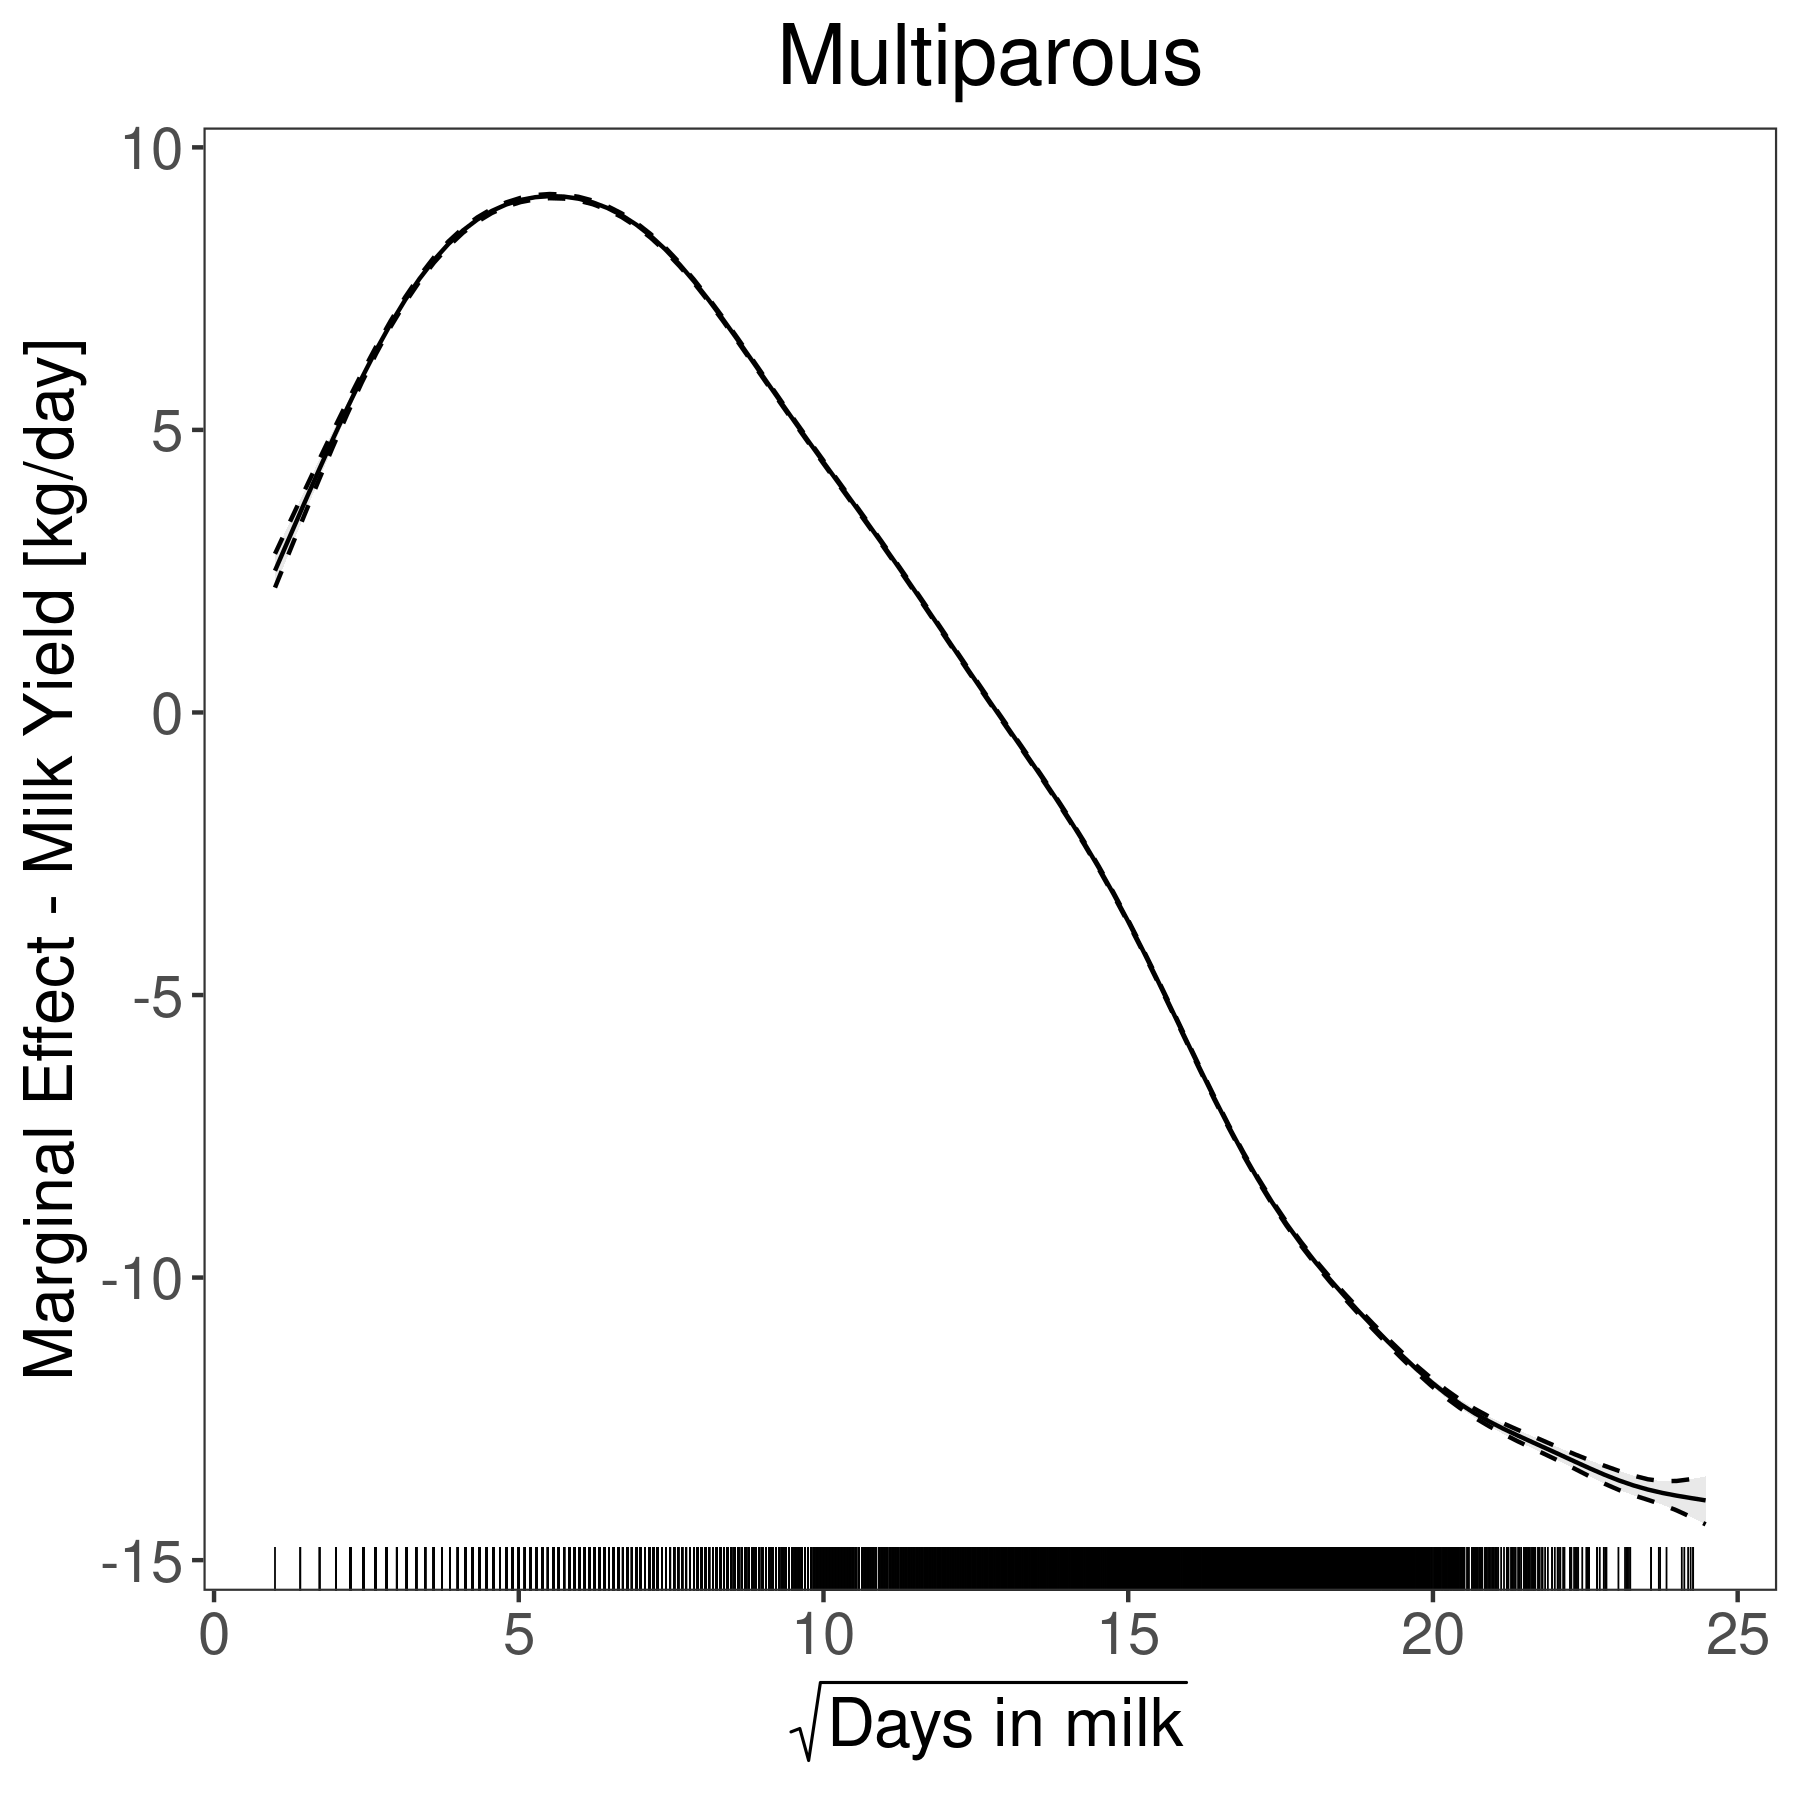
\includegraphics[width=\textwidth]{thesis/figures/models/milk/full/ho_milk_full/ho_milk_full_marginal_dim_milk_multi.png}
    \end{subfigure}
    \caption[]{Holstein: Milk Yield - 1985 - 2023 - THI Effect and Lactation Curve}
    \label{fig:main}
\end{figure}

\subsection{Split Period: Until 2010 - After 2010}
\addtocontents{toc}{\protect\setcounter{tocdepth}{-1}}
\subsubsection{Split Period: 1985 - 2010}\label{model:ho_milk_before}
\paragraph{Model Summary} \quad \\

    \begin{table}[H]
    \centering
    \begin{tabular}{lrrrr}
    \textbf{A. parametric coefficients} & Estimate & Std. Error & t-value & p-value \\ 
       \hline
       \hline
  (Intercept) & 17.4723 & 0.4846 & 36.0518 & $<$ 0.0001 \\ 
  parityprimiparous & -2.9636 & 0.0135 & -218.8244 & $<$ 0.0001 \\ 
  year1986 & 0.1529 & 0.1767 & 0.8655 & 0.3868 \\ 
  year1987 & -0.0051 & 0.3698 & -0.0139 & 0.9889 \\ 
  year1988 & -0.0538 & 0.4676 & -0.1151 & 0.9084 \\ 
  year1989 & 0.5836 & 0.5228 & 1.1162 & 0.2643 \\ 
  year1990 & 1.0427 & 0.5324 & 1.9586 & 0.0502 \\ 
  year1991 & 1.2681 & 0.5365 & 2.3638 & 0.0181 \\ 
  year1992 & 1.5385 & 0.5405 & 2.8462 & 0.0044 \\ 
  year1993 & 1.7418 & 0.5397 & 3.2271 & 0.0013 \\ 
  year1994 & 1.7286 & 0.5424 & 3.1867 & 0.0014 \\ 
  year1995 & 2.0734 & 0.5756 & 3.6019 & 0.0003 \\ 
  year1996 & 2.2707 & 0.5748 & 3.9506 & 0.0001 \\ 
  year1997 & 2.7340 & 0.5549 & 4.9272 & $<$ 0.0001 \\ 
  year1998 & 3.3217 & 0.5222 & 6.3608 & $<$ 0.0001 \\ 
  year1999 & 3.4296 & 0.5187 & 6.6121 & $<$ 0.0001 \\ 
  year2000 & 3.6071 & 0.5113 & 7.0543 & $<$ 0.0001 \\ 
  year2001 & 3.9367 & 0.5104 & 7.7127 & $<$ 0.0001 \\ 
  year2002 & 4.2369 & 0.5132 & 8.2562 & $<$ 0.0001 \\ 
  year2003 & 4.7670 & 0.5144 & 9.2674 & $<$ 0.0001 \\ 
  year2004 & 5.2638 & 0.5135 & 10.2511 & $<$ 0.0001 \\ 
  year2005 & 5.7675 & 0.5124 & 11.2567 & $<$ 0.0001 \\ 
  year2006 & 5.9112 & 0.5147 & 11.4841 & $<$ 0.0001 \\ 
  year2007 & 5.8929 & 0.5097 & 11.5607 & $<$ 0.0001 \\ 
  year2008 & 6.2882 & 0.4996 & 12.5867 & $<$ 0.0001 \\ 
  year2009 & 6.9956 & 0.5079 & 13.7748 & $<$ 0.0001 \\ 
  year2010 & 7.7149 & 0.5678 & 13.5864 & $<$ 0.0001 \\ 
       \hline
    \textbf{B. smooth terms} & edf & Ref.df & F-value & p-value \\ 
    \hline
    \hline
  s(thi\_mean\_t0\_3d):paritymultiparous & 8.5121 & 8.5121 & 747.8886 & $<$ 0.0001 \\ 
  s(thi\_mean\_t0\_3d):parityprimiparous & 7.1550 & 7.1550 & 77.0589 & $<$ 0.0001 \\ 
  s(days\_in\_milk\_t):paritymultiparous & 14.4063 & 14.4063 & 130999.6058 & $<$ 0.0001 \\ 
  s(days\_in\_milk\_t):parityprimiparous & 13.8961 & 13.8961 & 17856.8448 & $<$ 0.0001 \\ 
       \hline
    \end{tabular}
    \caption[]{Holstein: Milk Yield - 1985-2010 - GAMM model summary without random effect terms.}
    \end{table}

\newpage
\begin{table}[H]
\centering
\begin{tabular}
{l | r | r | r | r}
\textbf{Smooth Term Fixed Effect} & Est. & SE & z & p\\
\hline
\hline
s(thi\_mean\_t0\_3d):multiFx1 & -0.5301 & 0.1141 & -4.65 & $<$ 1e-05\\
s(thi\_mean\_t0\_3d):primiFx1 & -0.3337 & 0.1241 & -2.69 & 0.0072\\
s(days\_in\_milk\_):multiFx1 & 2.4075 & 0.5902 & 4.08 & $<$ 1e-04\\
s(days\_in\_milk\_):primiFx1 & 2.9462 & 0.6274 & 4.70 & $<$ 1e-05\\
\hline
\textbf{Variance Component} & Estimated $\sigma$ & & & \\
\hline
\hline
$\sigma_\alpha$ & 2.9738 & &  & \\
$\sigma_\iota$ & 0.9483 & & & \\
$\sigma_\phi$ & 2.7446 & & & \\
s(thi\_mean\_t0\_3d):multi & 2.7246 & & & \\
s(days\_in\_milk\_):primi & 7.6254 & & & \\
s(days\_in\_milk\_):multi & 9.4602 & & & \\
s(thi\_mean\_t0\_3d):primi & 1.5465 & & & \\
Residual & 3.4568 & & & \\
\end{tabular}
\caption[]{Holstein: Milk Yield - 1985-2010 - Mixed Model Summary - Smooth Terms and Random Effects.}
\end{table}

\paragraph{Model Diagnostics} \quad \\
\begin{figure}[H]
    \centering
    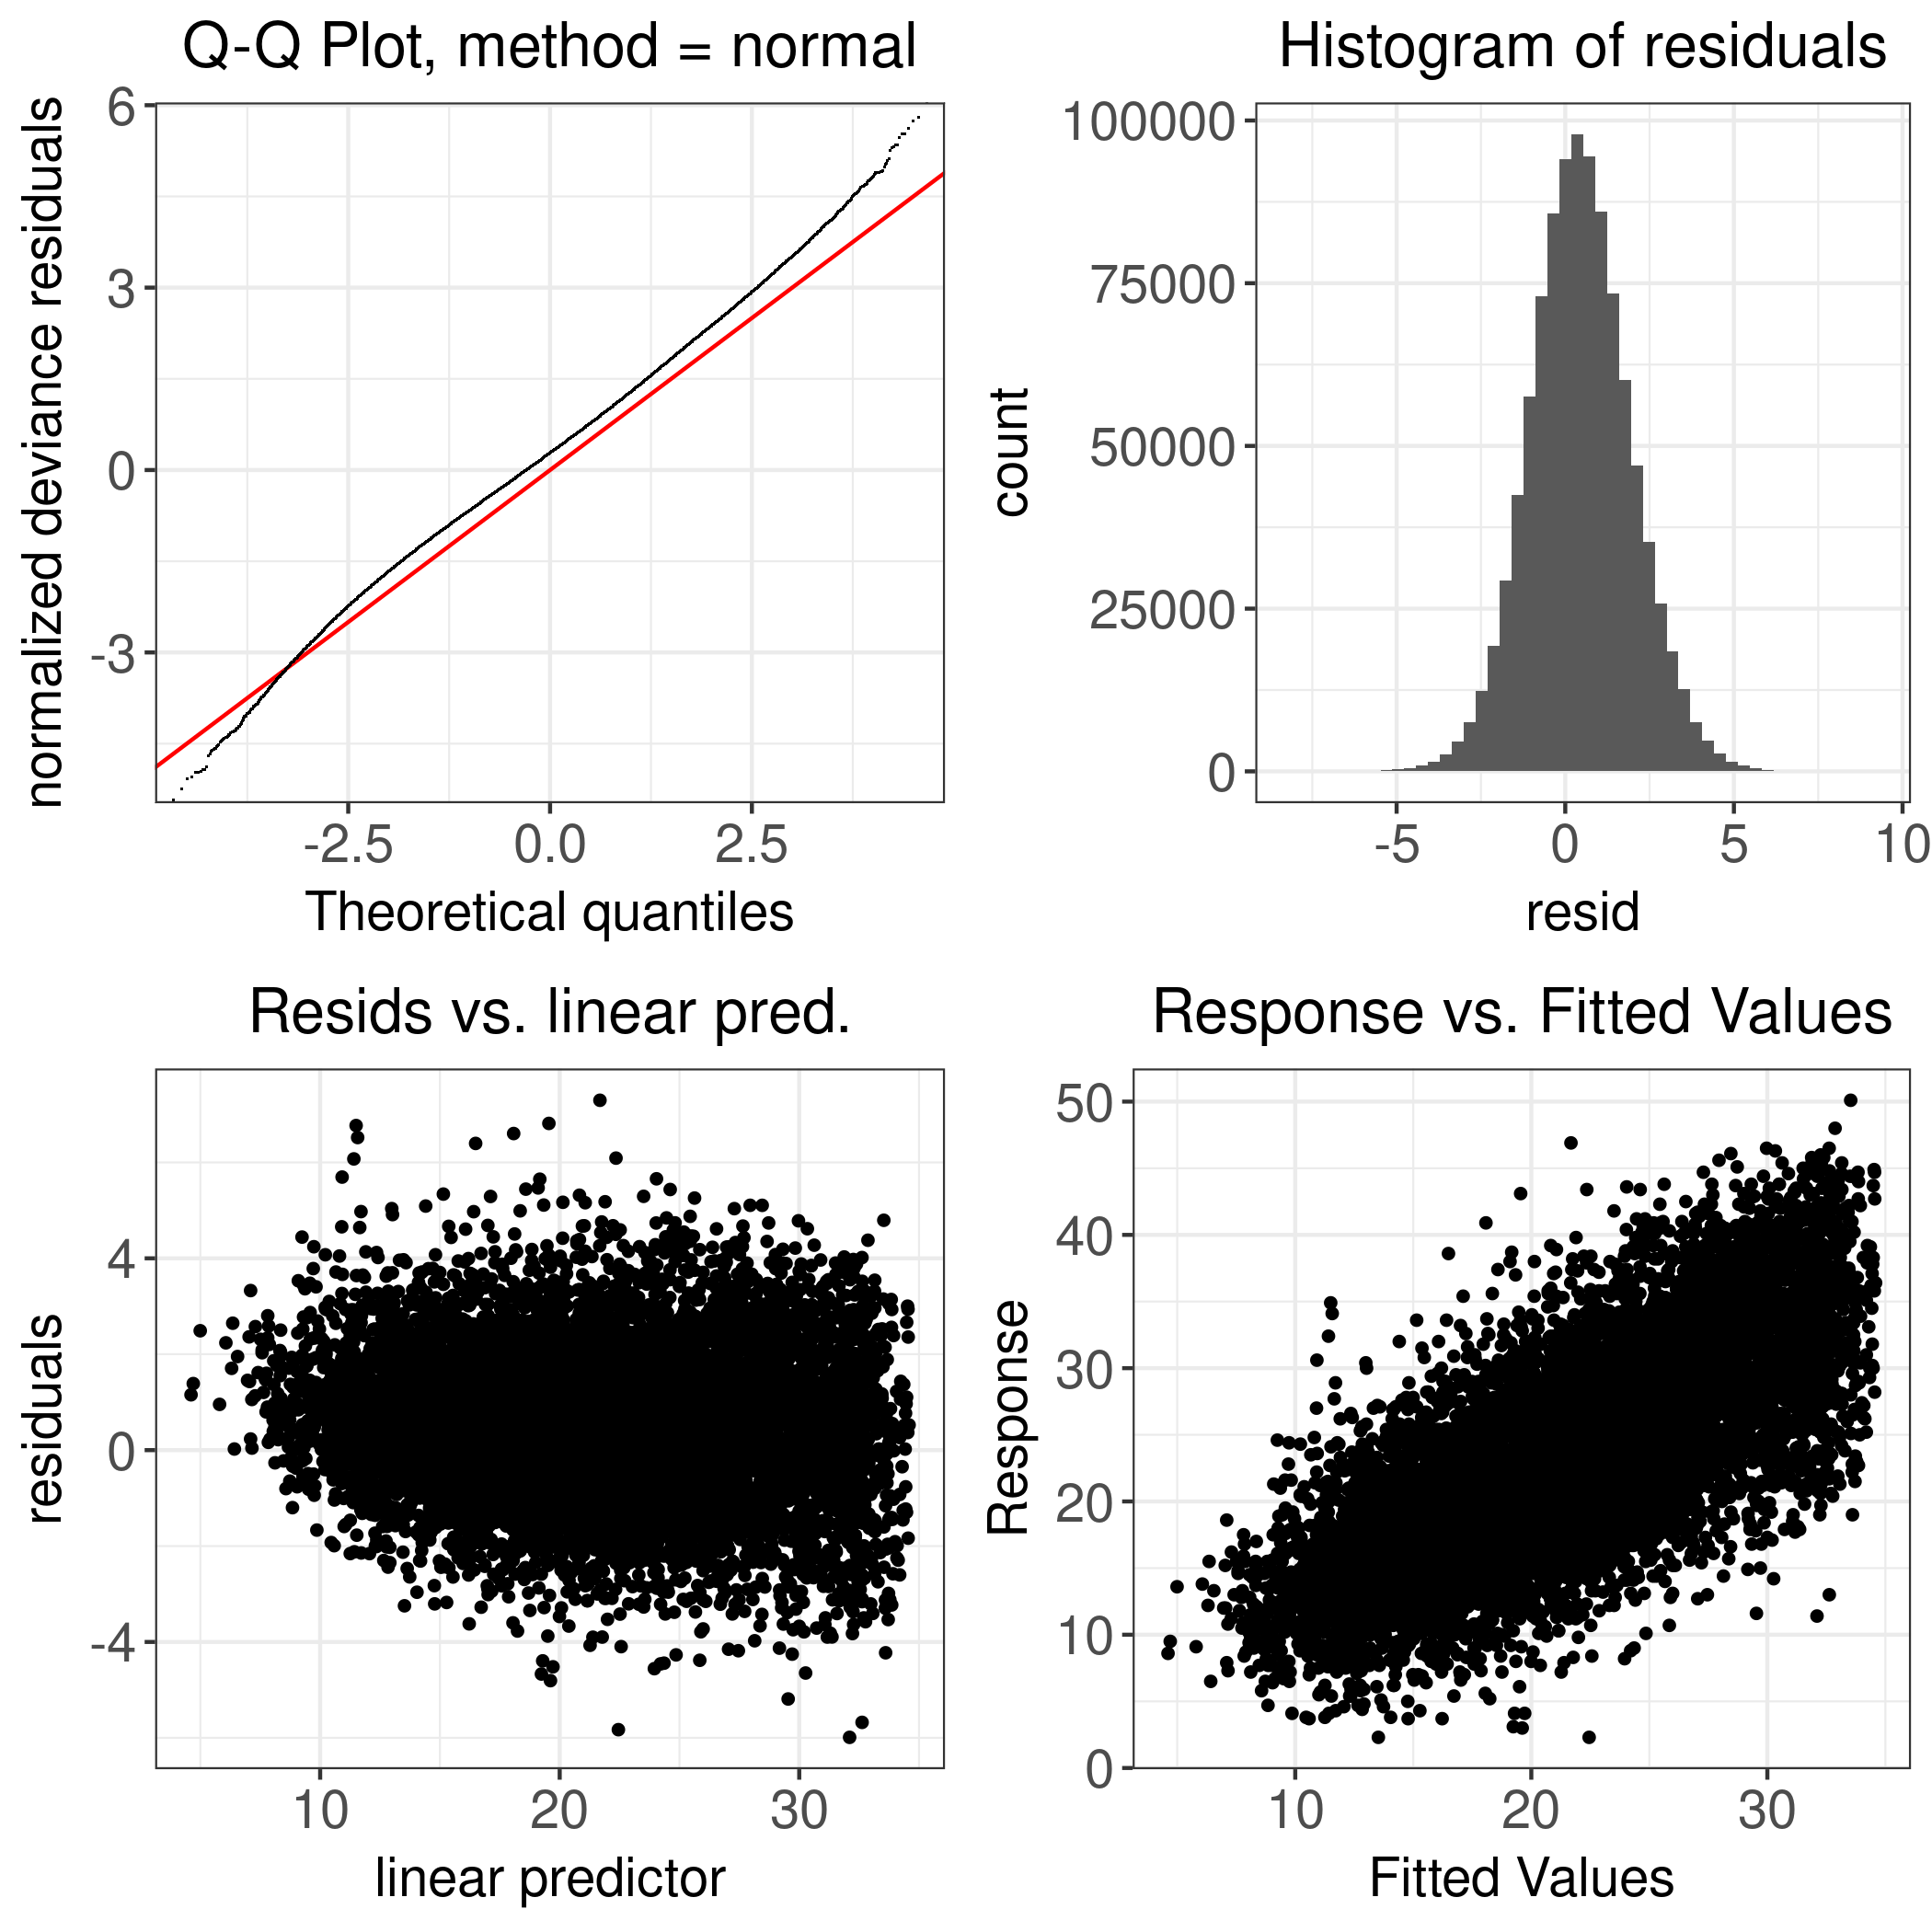
\includegraphics[width=0.6\textwidth]{thesis/figures/models/milk/before2010/ho_milk_before2010/ho_milk_before2010_diagnostics.png}
    \caption[]{Holstein: Milk Yield - 1985-2010 - Diagnostic Plot}
\end{figure}

\newpage
\paragraph{THI Effect and Lactation Curve} \quad \\
\begin{figure}[H]
    \centering
    \begin{subfigure}[b]{0.45\textwidth}
        \centering
        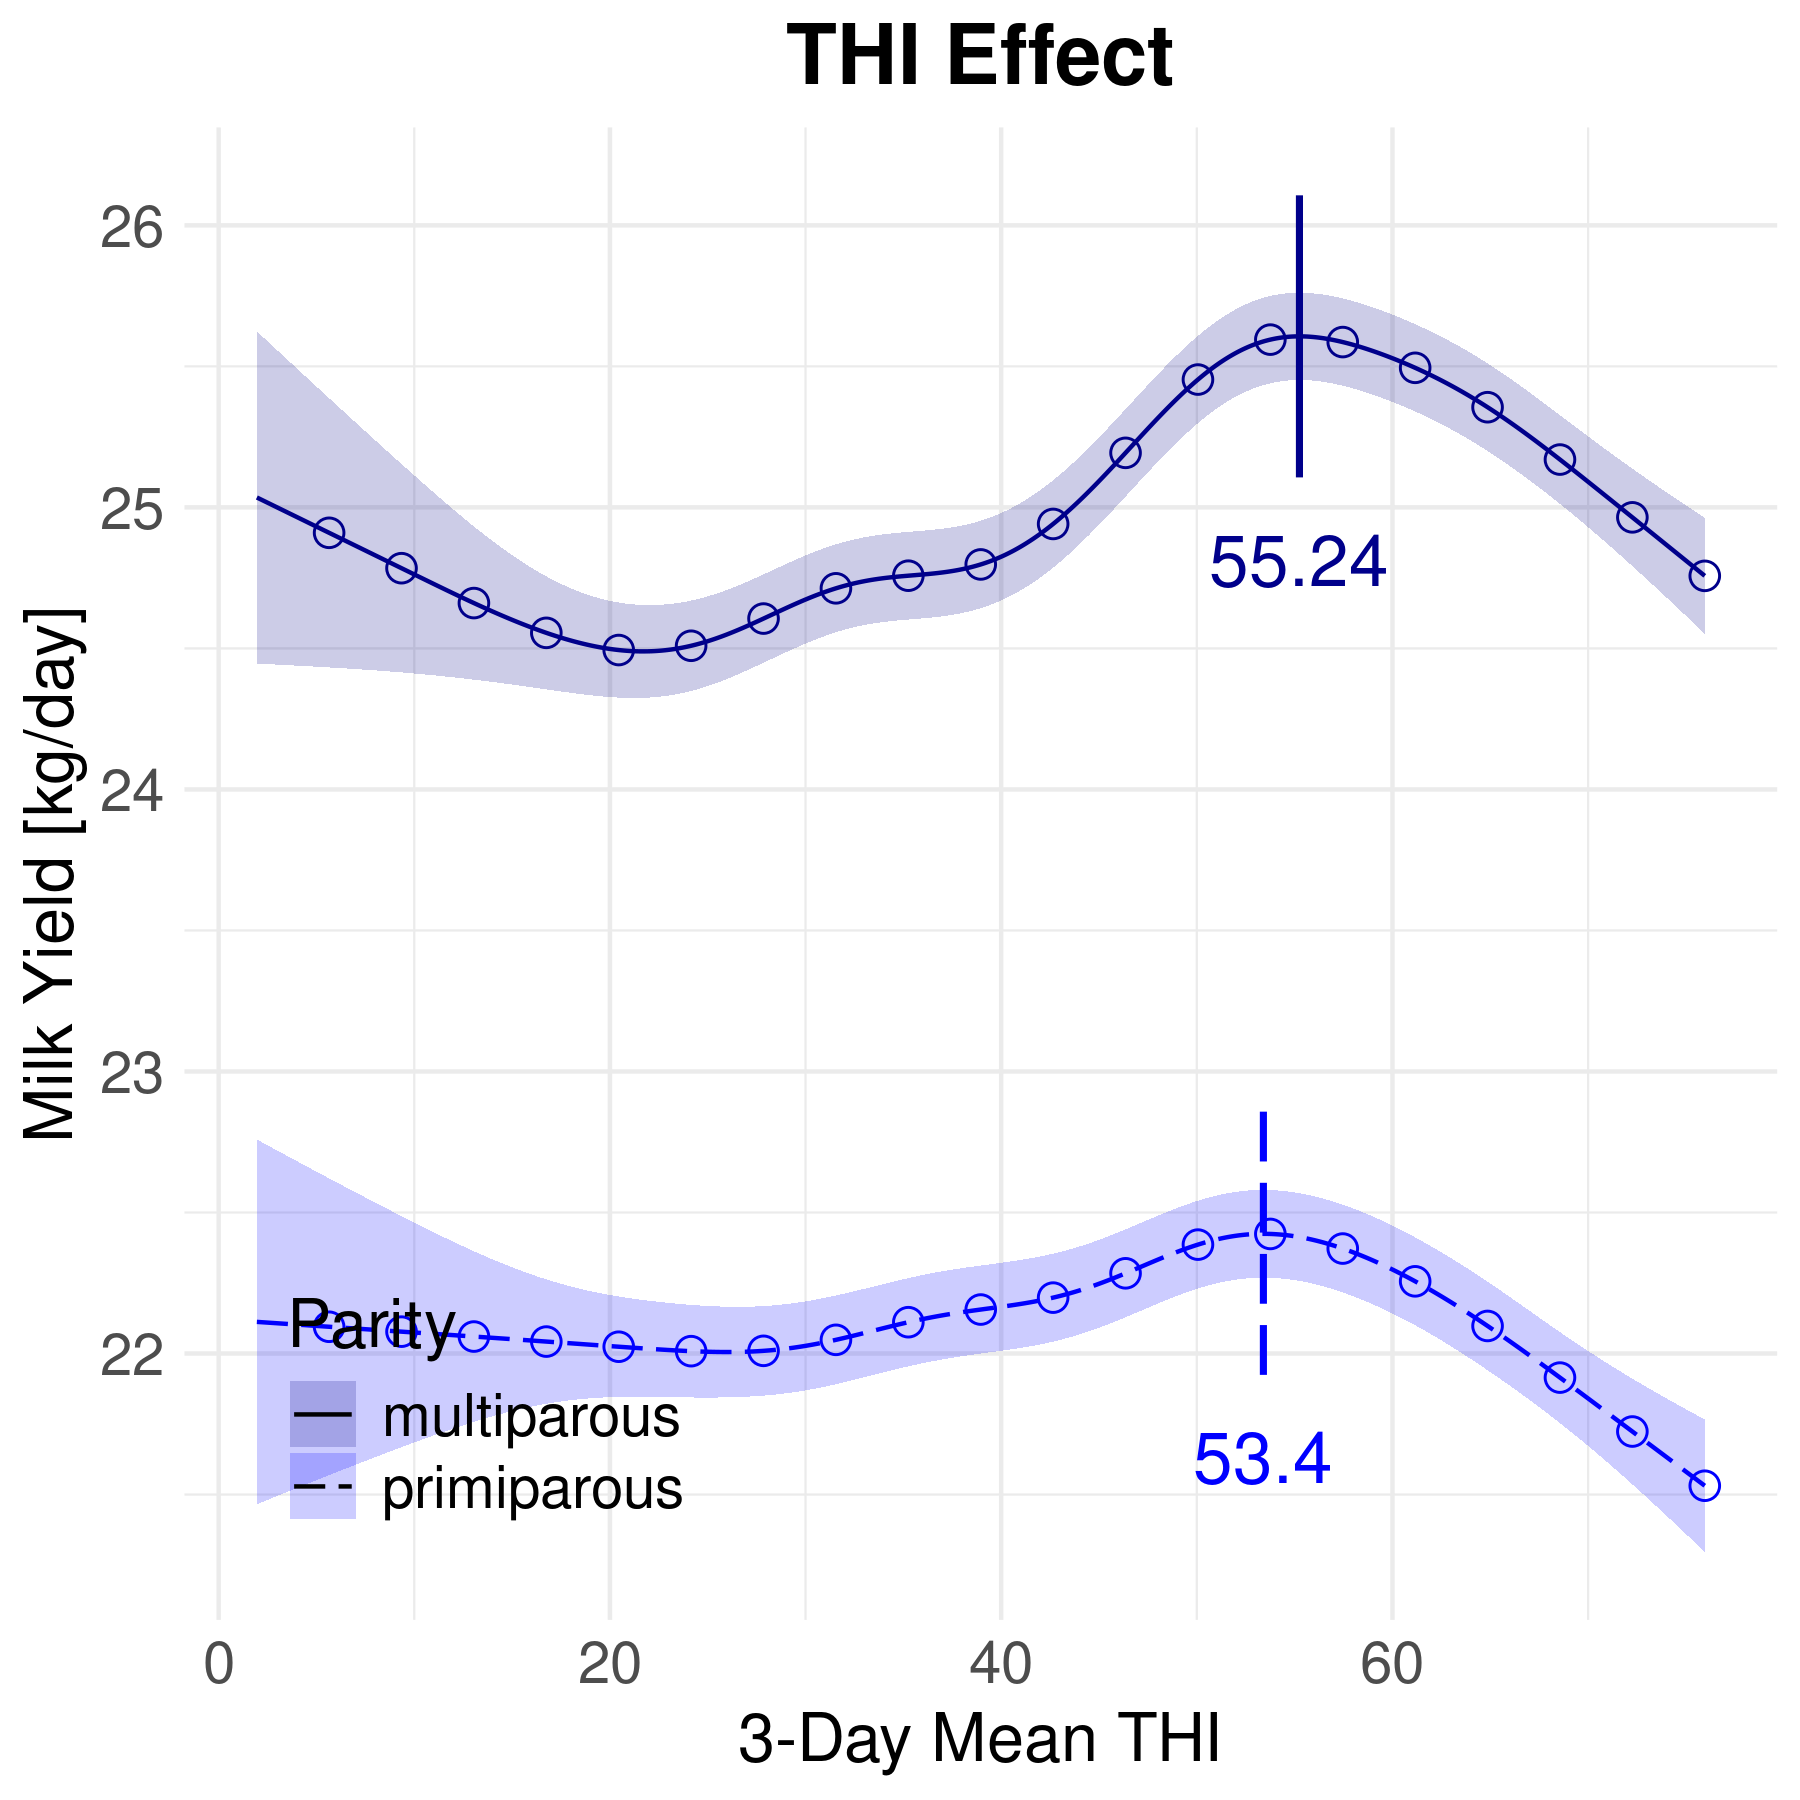
\includegraphics[width=\textwidth]{thesis/figures/models/milk/before2010/ho_milk_before2010/ho_milk_before2010_marginal_thi_milk_combined.png}
    \end{subfigure}
    \hspace{0.05\textwidth} % Optional space between the figures
    \begin{subfigure}[b]{0.45\textwidth}
        \centering
        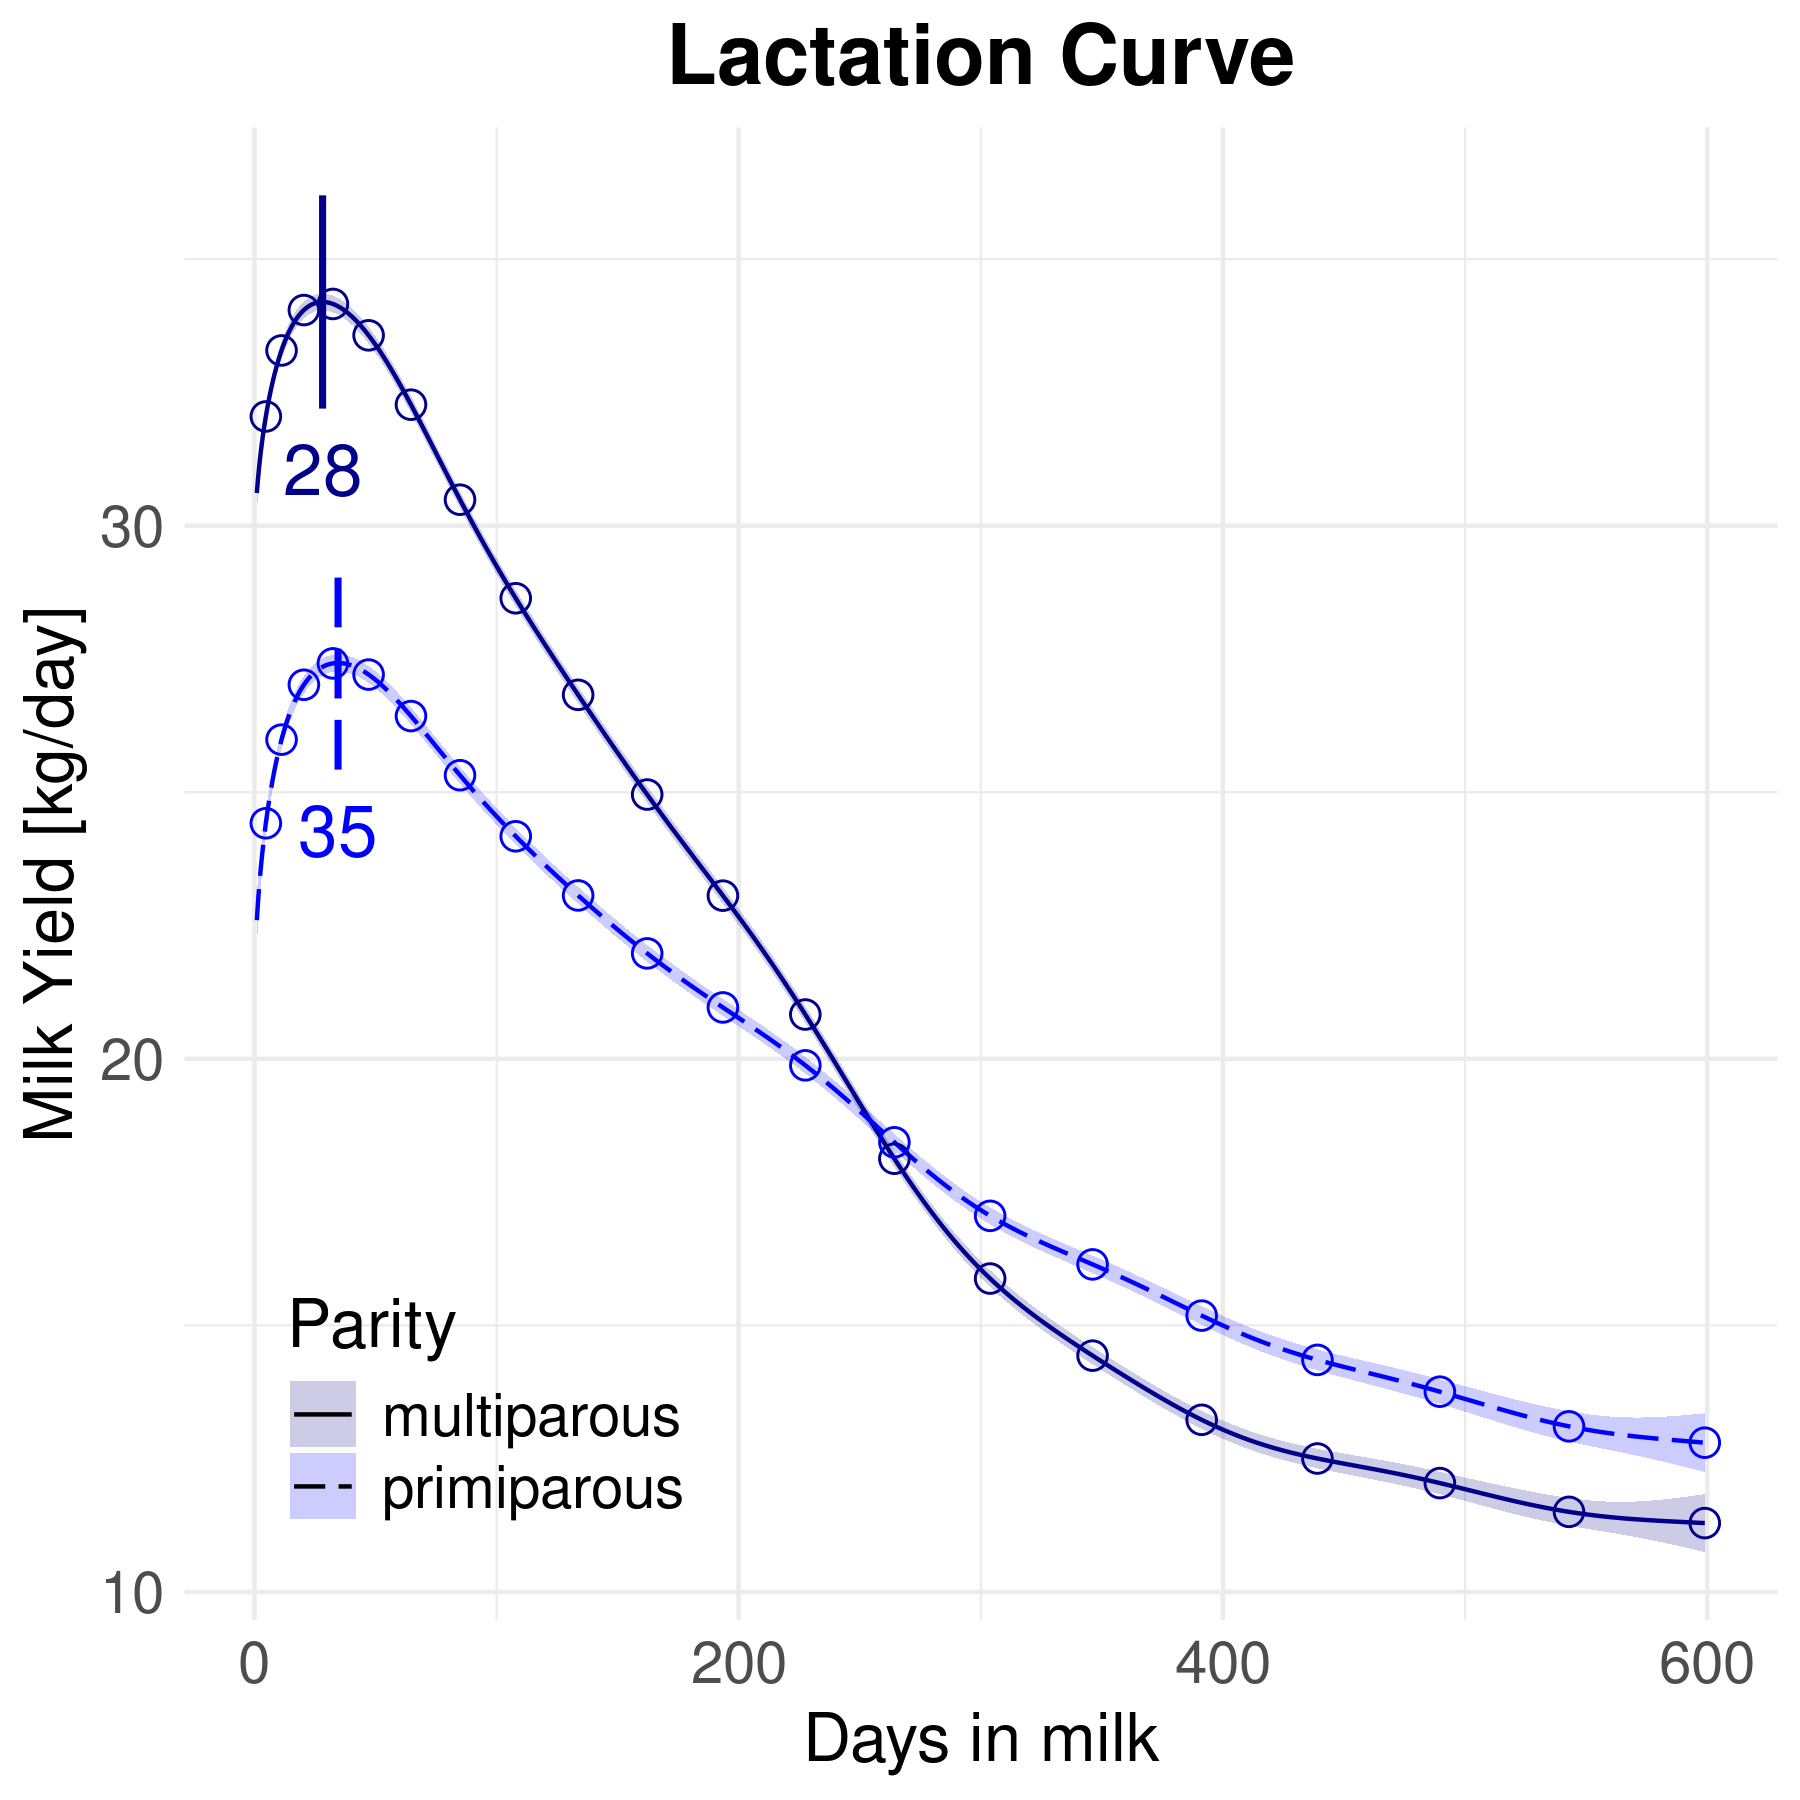
\includegraphics[width=\textwidth]{thesis/figures/models/milk/before2010/ho_milk_before2010/ho_milk_before2010_marginal_dim_milk_combined.png}
    \end{subfigure}
    \begin{subfigure}[b]{0.45\textwidth}
        \centering
        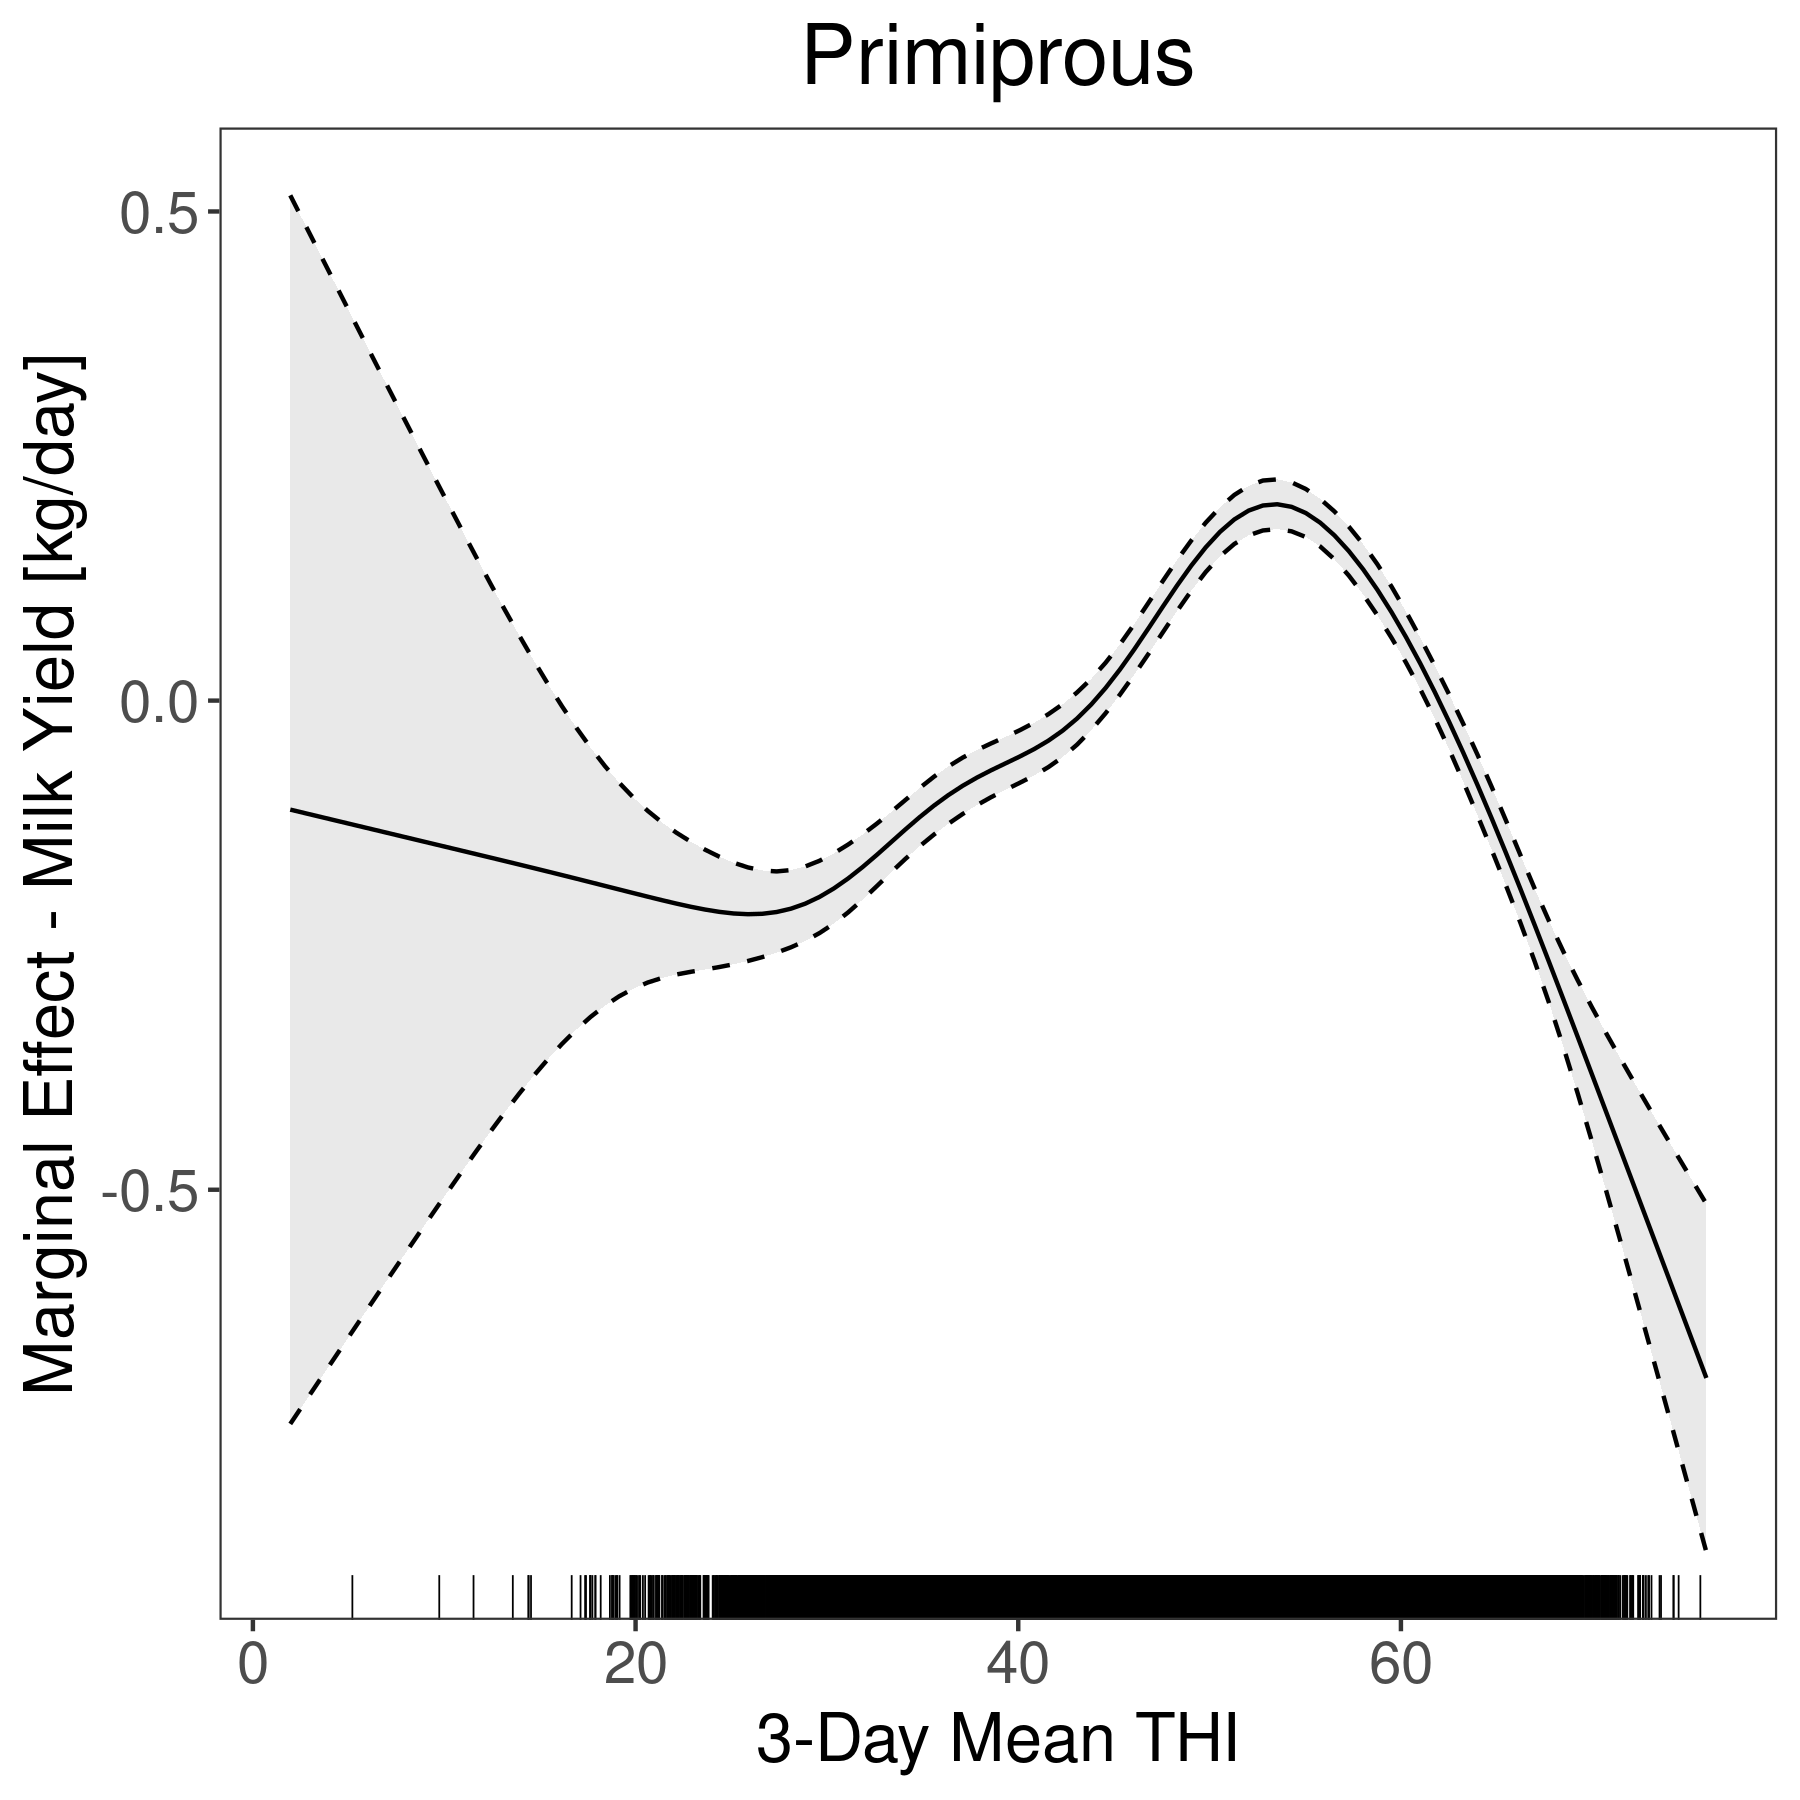
\includegraphics[width=\textwidth]{thesis/figures/models/milk/before2010/ho_milk_before2010/ho_milk_before2010_marginal_thi_milk_primi.png}
    \end{subfigure}
    \hspace{0.05\textwidth} % Optional space between the figures
    \begin{subfigure}[b]{0.45\textwidth}
        \centering
        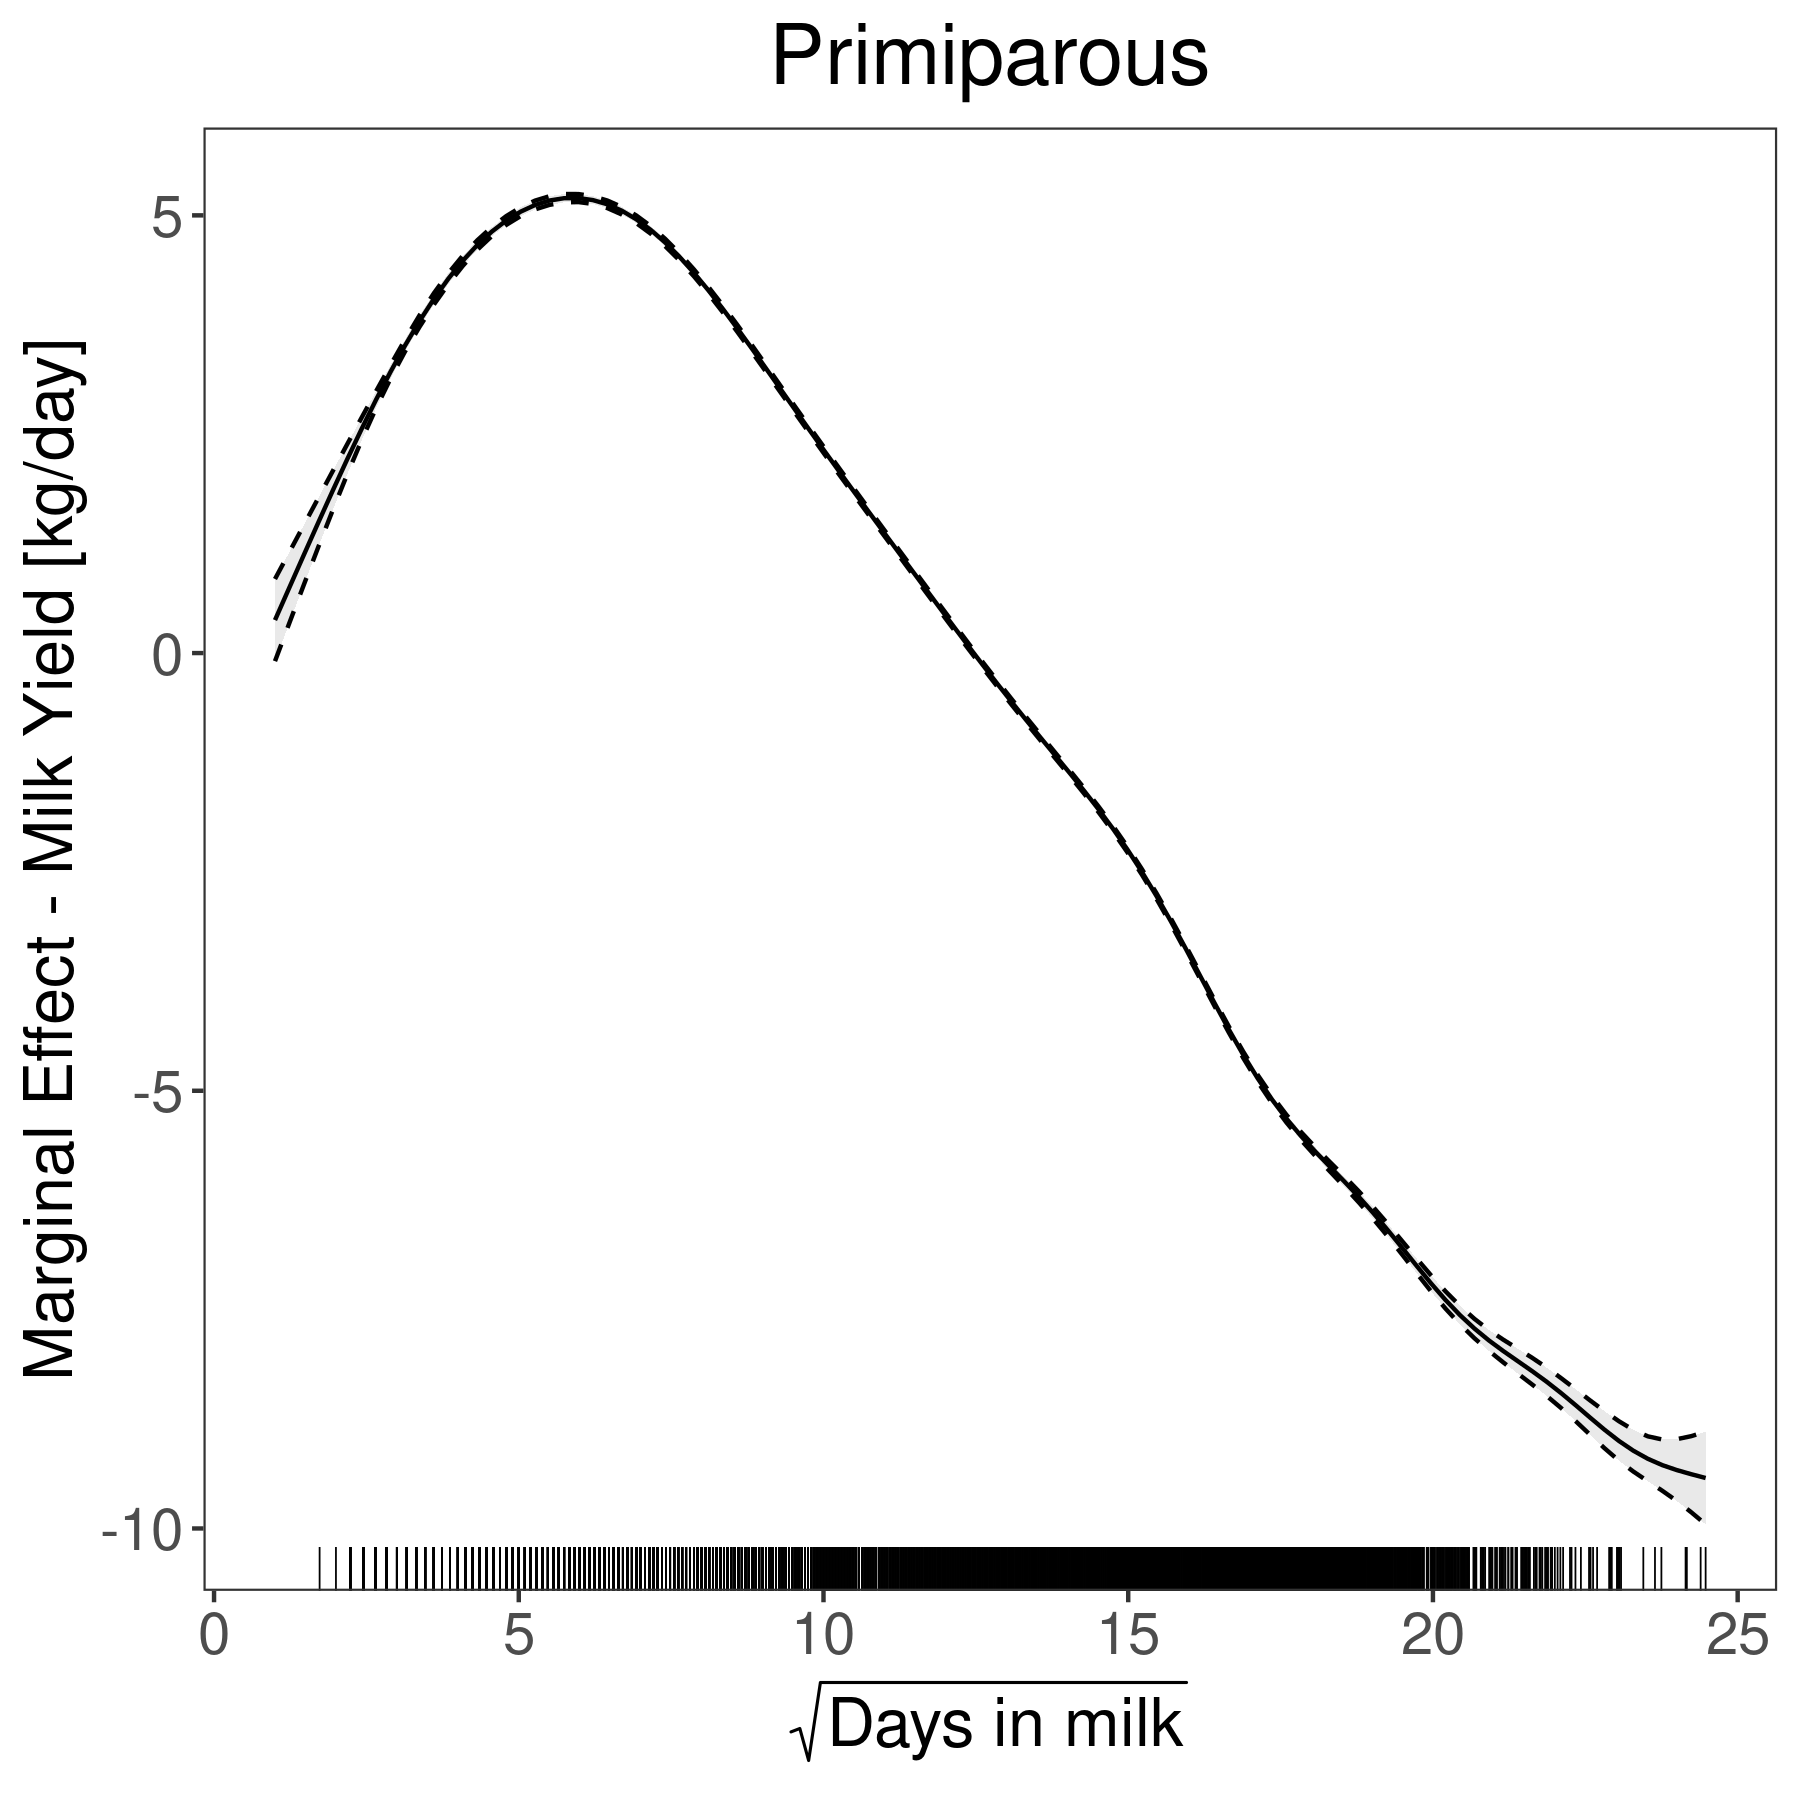
\includegraphics[width=\textwidth]{thesis/figures/models/milk/before2010/ho_milk_before2010/ho_milk_before2010_marginal_dim_milk_primi.png}
    \end{subfigure}
    \begin{subfigure}[b]{0.45\textwidth}
        \centering
        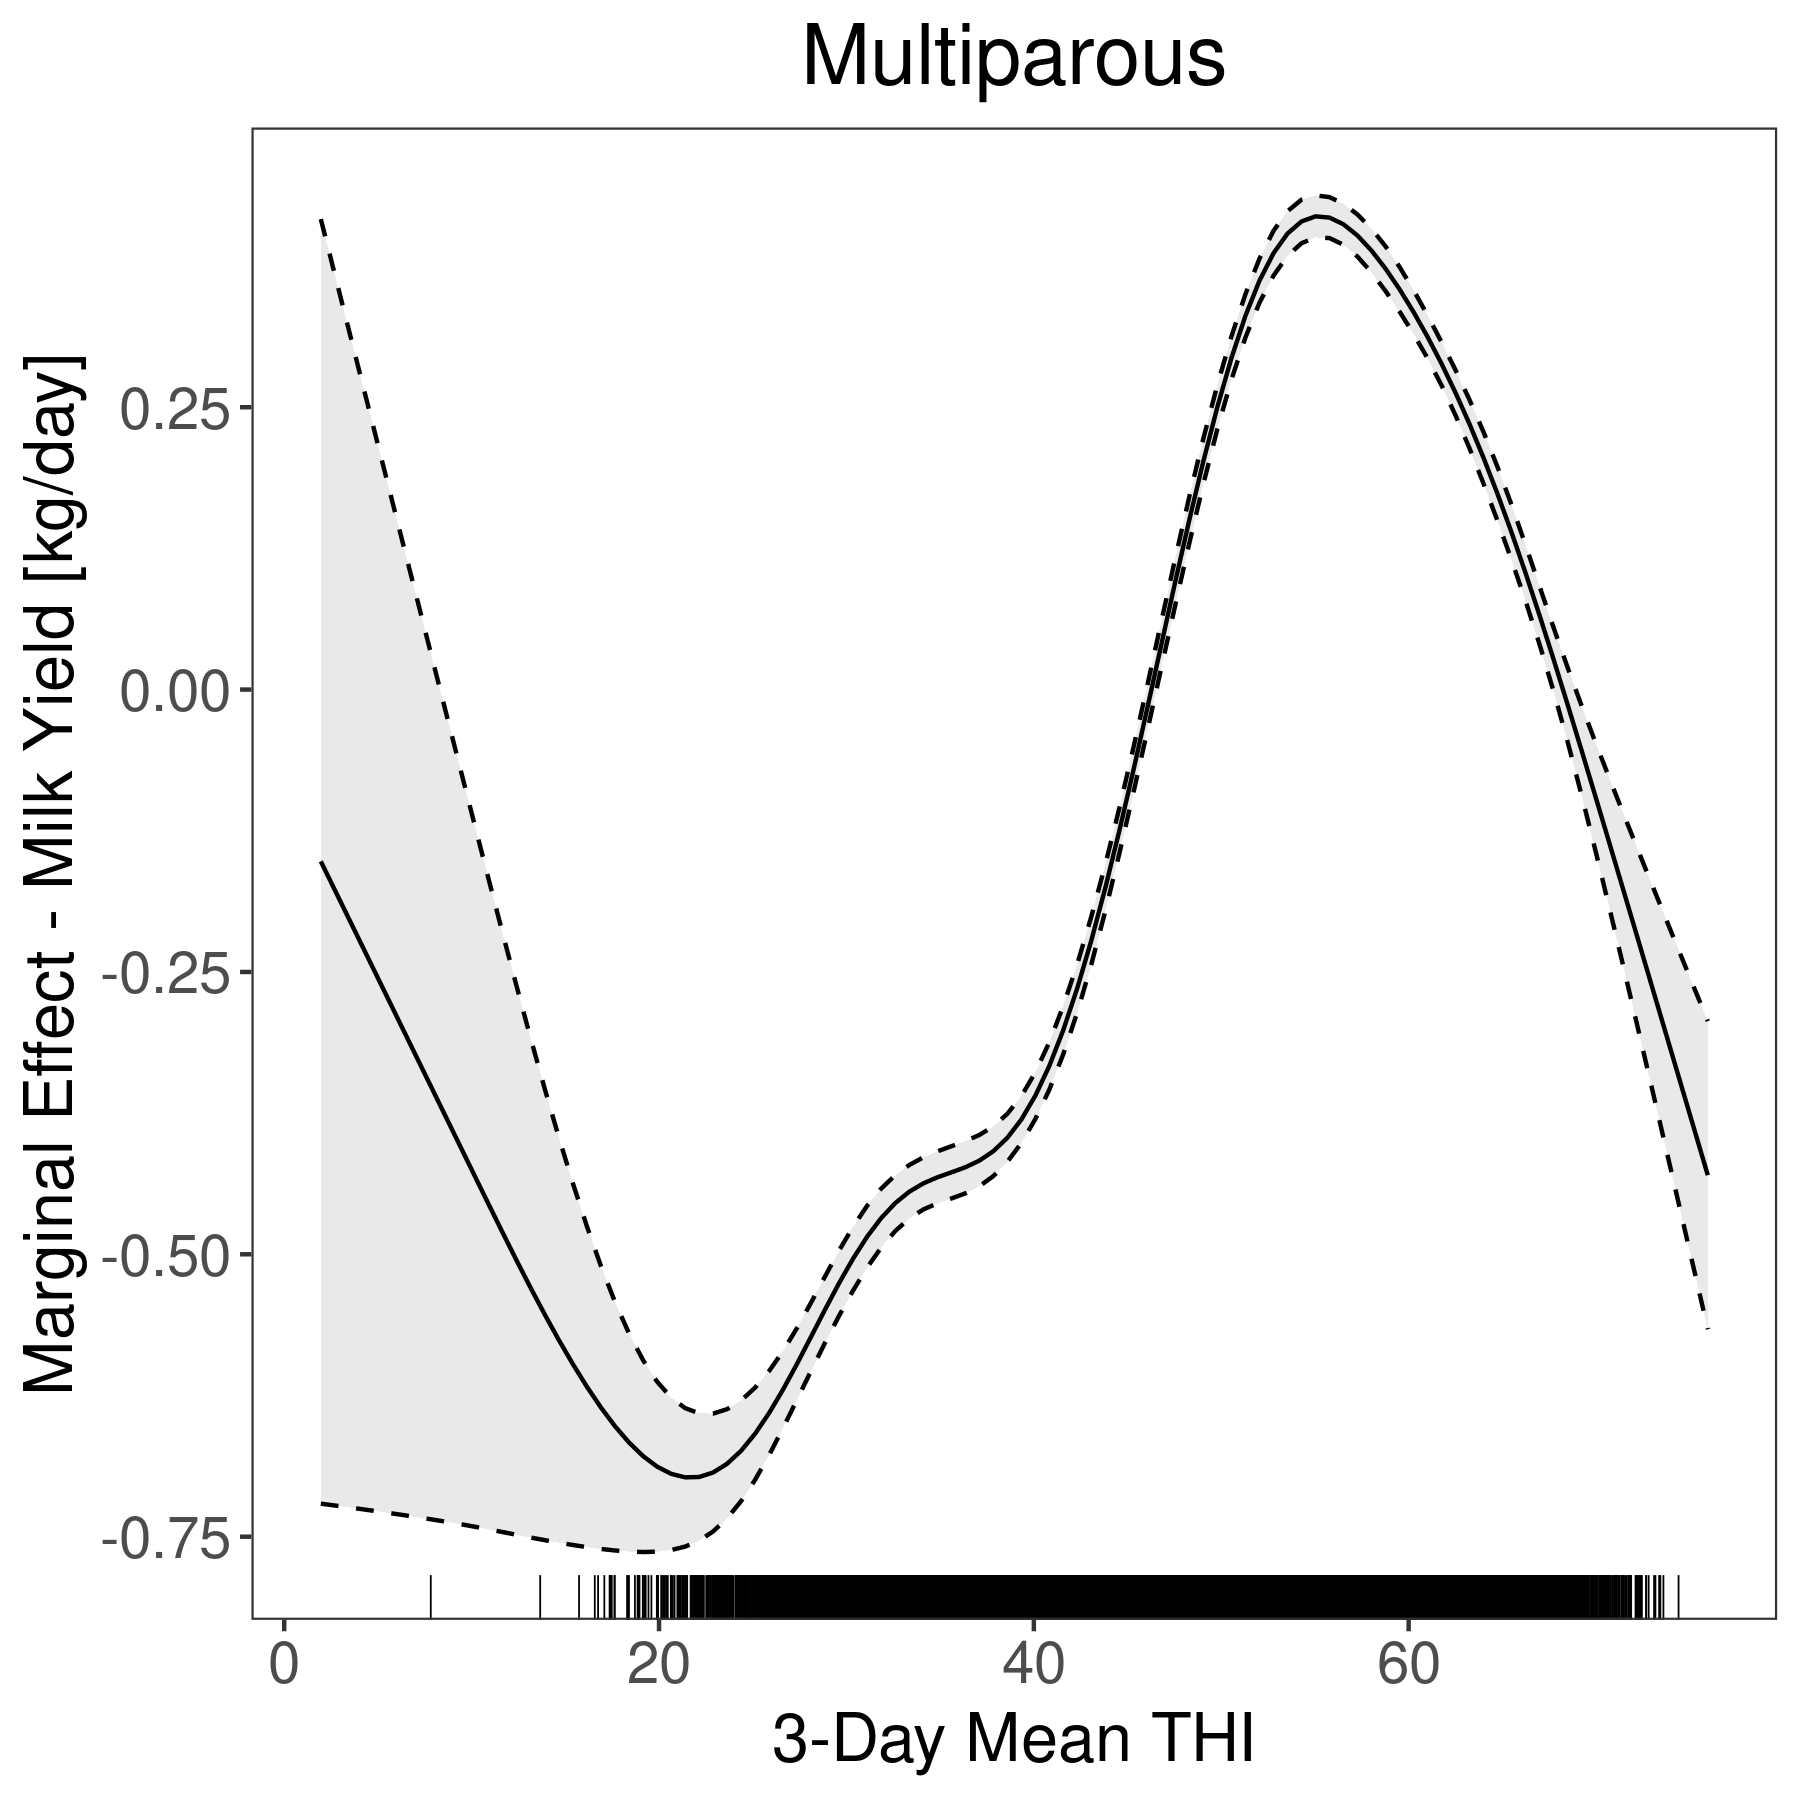
\includegraphics[width=\textwidth]{thesis/figures/models/milk/before2010/ho_milk_before2010/ho_milk_before2010_marginal_thi_milk_multi.png}
    \end{subfigure}
    \hspace{0.05\textwidth} % Optional space between the figures
    \begin{subfigure}[b]{0.45\textwidth}
        \centering
        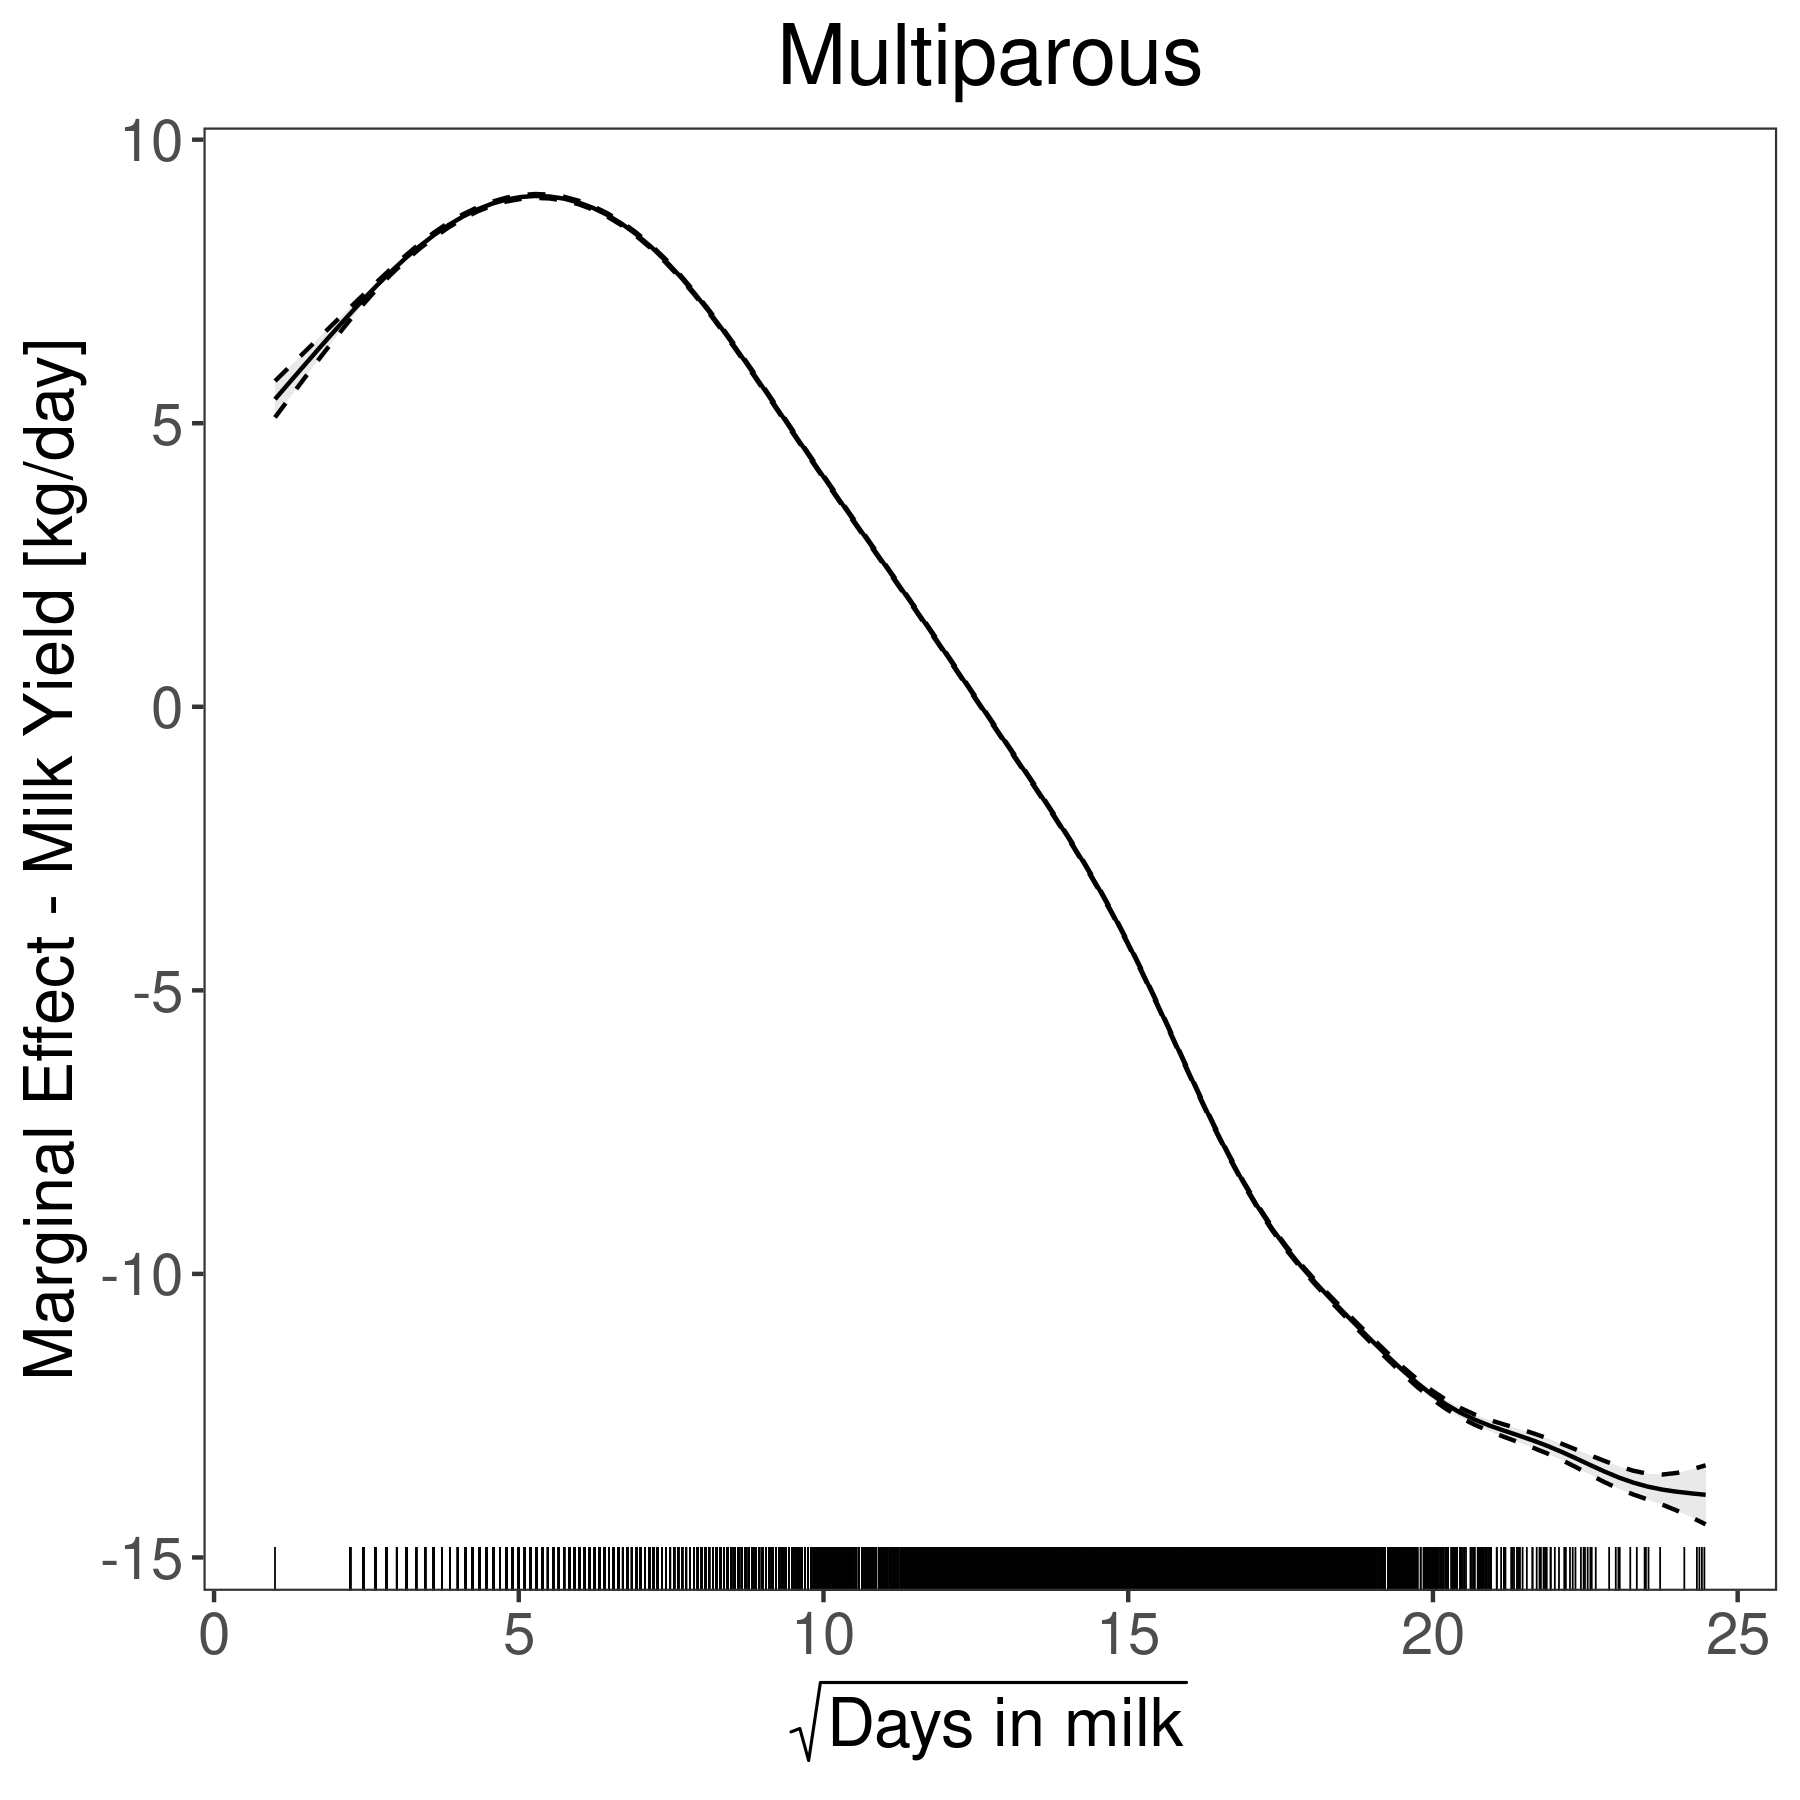
\includegraphics[width=\textwidth]{thesis/figures/models/milk/before2010/ho_milk_before2010/ho_milk_before2010_marginal_dim_milk_multi.png}
    \end{subfigure}
    \caption[]{Holstein: Milk Yield - 1985 - 2010 - THI Effect and Lactation Curve}
    \label{fig:main}
\end{figure}

\subsubsection{Split Period: 2010 - 2023}\label{model:ho_milk_after}

\paragraph{Model Summary} \quad \\

    \begin{table}[H]
    \centering
    \begin{tabular}{lrrrr}
    \textbf{A. parametric coefficients} & Estimate & Std. Error & t-value & p-value \\ 
       \hline
       \hline
  (Intercept) & 23.8289 & 0.3841 & 62.0385 & $<$ 0.0001 \\ 
  parityprimiparous & -3.5815 & 0.0143 & -250.7346 & $<$ 0.0001 \\ 
  year2012 & -0.1435 & 0.4281 & -0.3352 & 0.7375 \\ 
  year2013 & -0.4446 & 0.4293 & -1.0358 & 0.3003 \\ 
  year2014 & 0.1502 & 0.4291 & 0.3501 & 0.7263 \\ 
  year2015 & 0.4723 & 0.4308 & 1.0965 & 0.2728 \\ 
  year2016 & 0.7635 & 0.4567 & 1.6718 & 0.0946 \\ 
  year2017 & 1.1762 & 0.4488 & 2.6207 & 0.0088 \\ 
  year2018 & 1.7098 & 0.4437 & 3.8535 & 0.0001 \\ 
  year2019 & 1.9267 & 0.4429 & 4.3500 & $<$ 0.0001 \\ 
  year2020 & 2.4354 & 0.4451 & 5.4719 & $<$ 0.0001 \\ 
  year2021 & 2.6773 & 0.4567 & 5.8617 & $<$ 0.0001 \\ 
  year2022 & 2.5650 & 0.4533 & 5.6584 & $<$ 0.0001 \\ 
  year2023 & 2.9380 & 0.4808 & 6.1102 & $<$ 0.0001 \\ 
       \hline
    \textbf{B. smooth terms} & edf & Ref.df & F-value & p-value \\ 
    \hline
    \hline
  s(thi\_mean\_t0\_3d):paritymultiparous & 8.3215 & 8.3215 & 484.5057 & $<$ 0.0001 \\ 
  s(thi\_mean\_t0\_3d):parityprimiparous & 7.0657 & 7.0657 & 29.5389 & $<$ 0.0001 \\ 
  s(days\_in\_milk\_t):paritymultiparous & 14.6827 & 14.6827 & 114849.4858 & $<$ 0.0001 \\ 
  s(days\_in\_milk\_t):parityprimiparous & 13.9847 & 13.9847 & 12129.3973 & $<$ 0.0001 \\ 
       \hline
    \end{tabular}
    \caption[]{Holstein: Milk Yield - 2011-2023 - GAMM model summary without random effect terms.}
    \end{table}

\newpage
\begin{table}[H]
\centering
\begin{tabular}
{l | r | r | r | r}
\textbf{Smooth Term Fixed Effect} & Est. & SE & z & p\\
\hline
\hline
s(thi\_mean\_t0\_3d):multiFx1 & -0.5663 & 0.1050 & -5.39 & $<$ 1e-07\\
s(thi\_mean\_t0\_3d):primiFx1 & -0.4351 & 0.1310 & -3.32 & 0.0009\\
s(days\_in\_milk\_):multiFx1 & 6.2500 & 0.5244 & 11.92 & $<$ 1e-32\\
s(days\_in\_milk\_):primiFx1 &  3.9576 & 0.6407 & 6.18 & $<$ 1e-09\\
\hline
\textbf{Variance Component} & Estimated $\sigma$ & & & \\
\hline
\hline
$\sigma_\alpha$ & 3.1563 & &  & \\
$\sigma_\iota$ & 1.1935 & & & \\
$\sigma_\phi$ & 3.7462 & & & \\
s(thi\_mean\_t0\_3d):multi & 2.2598 & & & \\
s(days\_in\_milk\_):primi & 8.5279 & & & \\
s(days\_in\_milk\_):multi & 12.0097 & & & \\
s(thi\_mean\_t0\_3d):primi & 1.6772 & & & \\
Residual & 3.9639 & & & \\
\end{tabular}
\caption[]{Holstein: Milk Yield - 2011-2023 - Mixed Model Summary - Smooth Terms and Random Effects.}
\end{table}

\paragraph{Model Diagnostics} \quad \\
\begin{figure}[H]
    \centering
    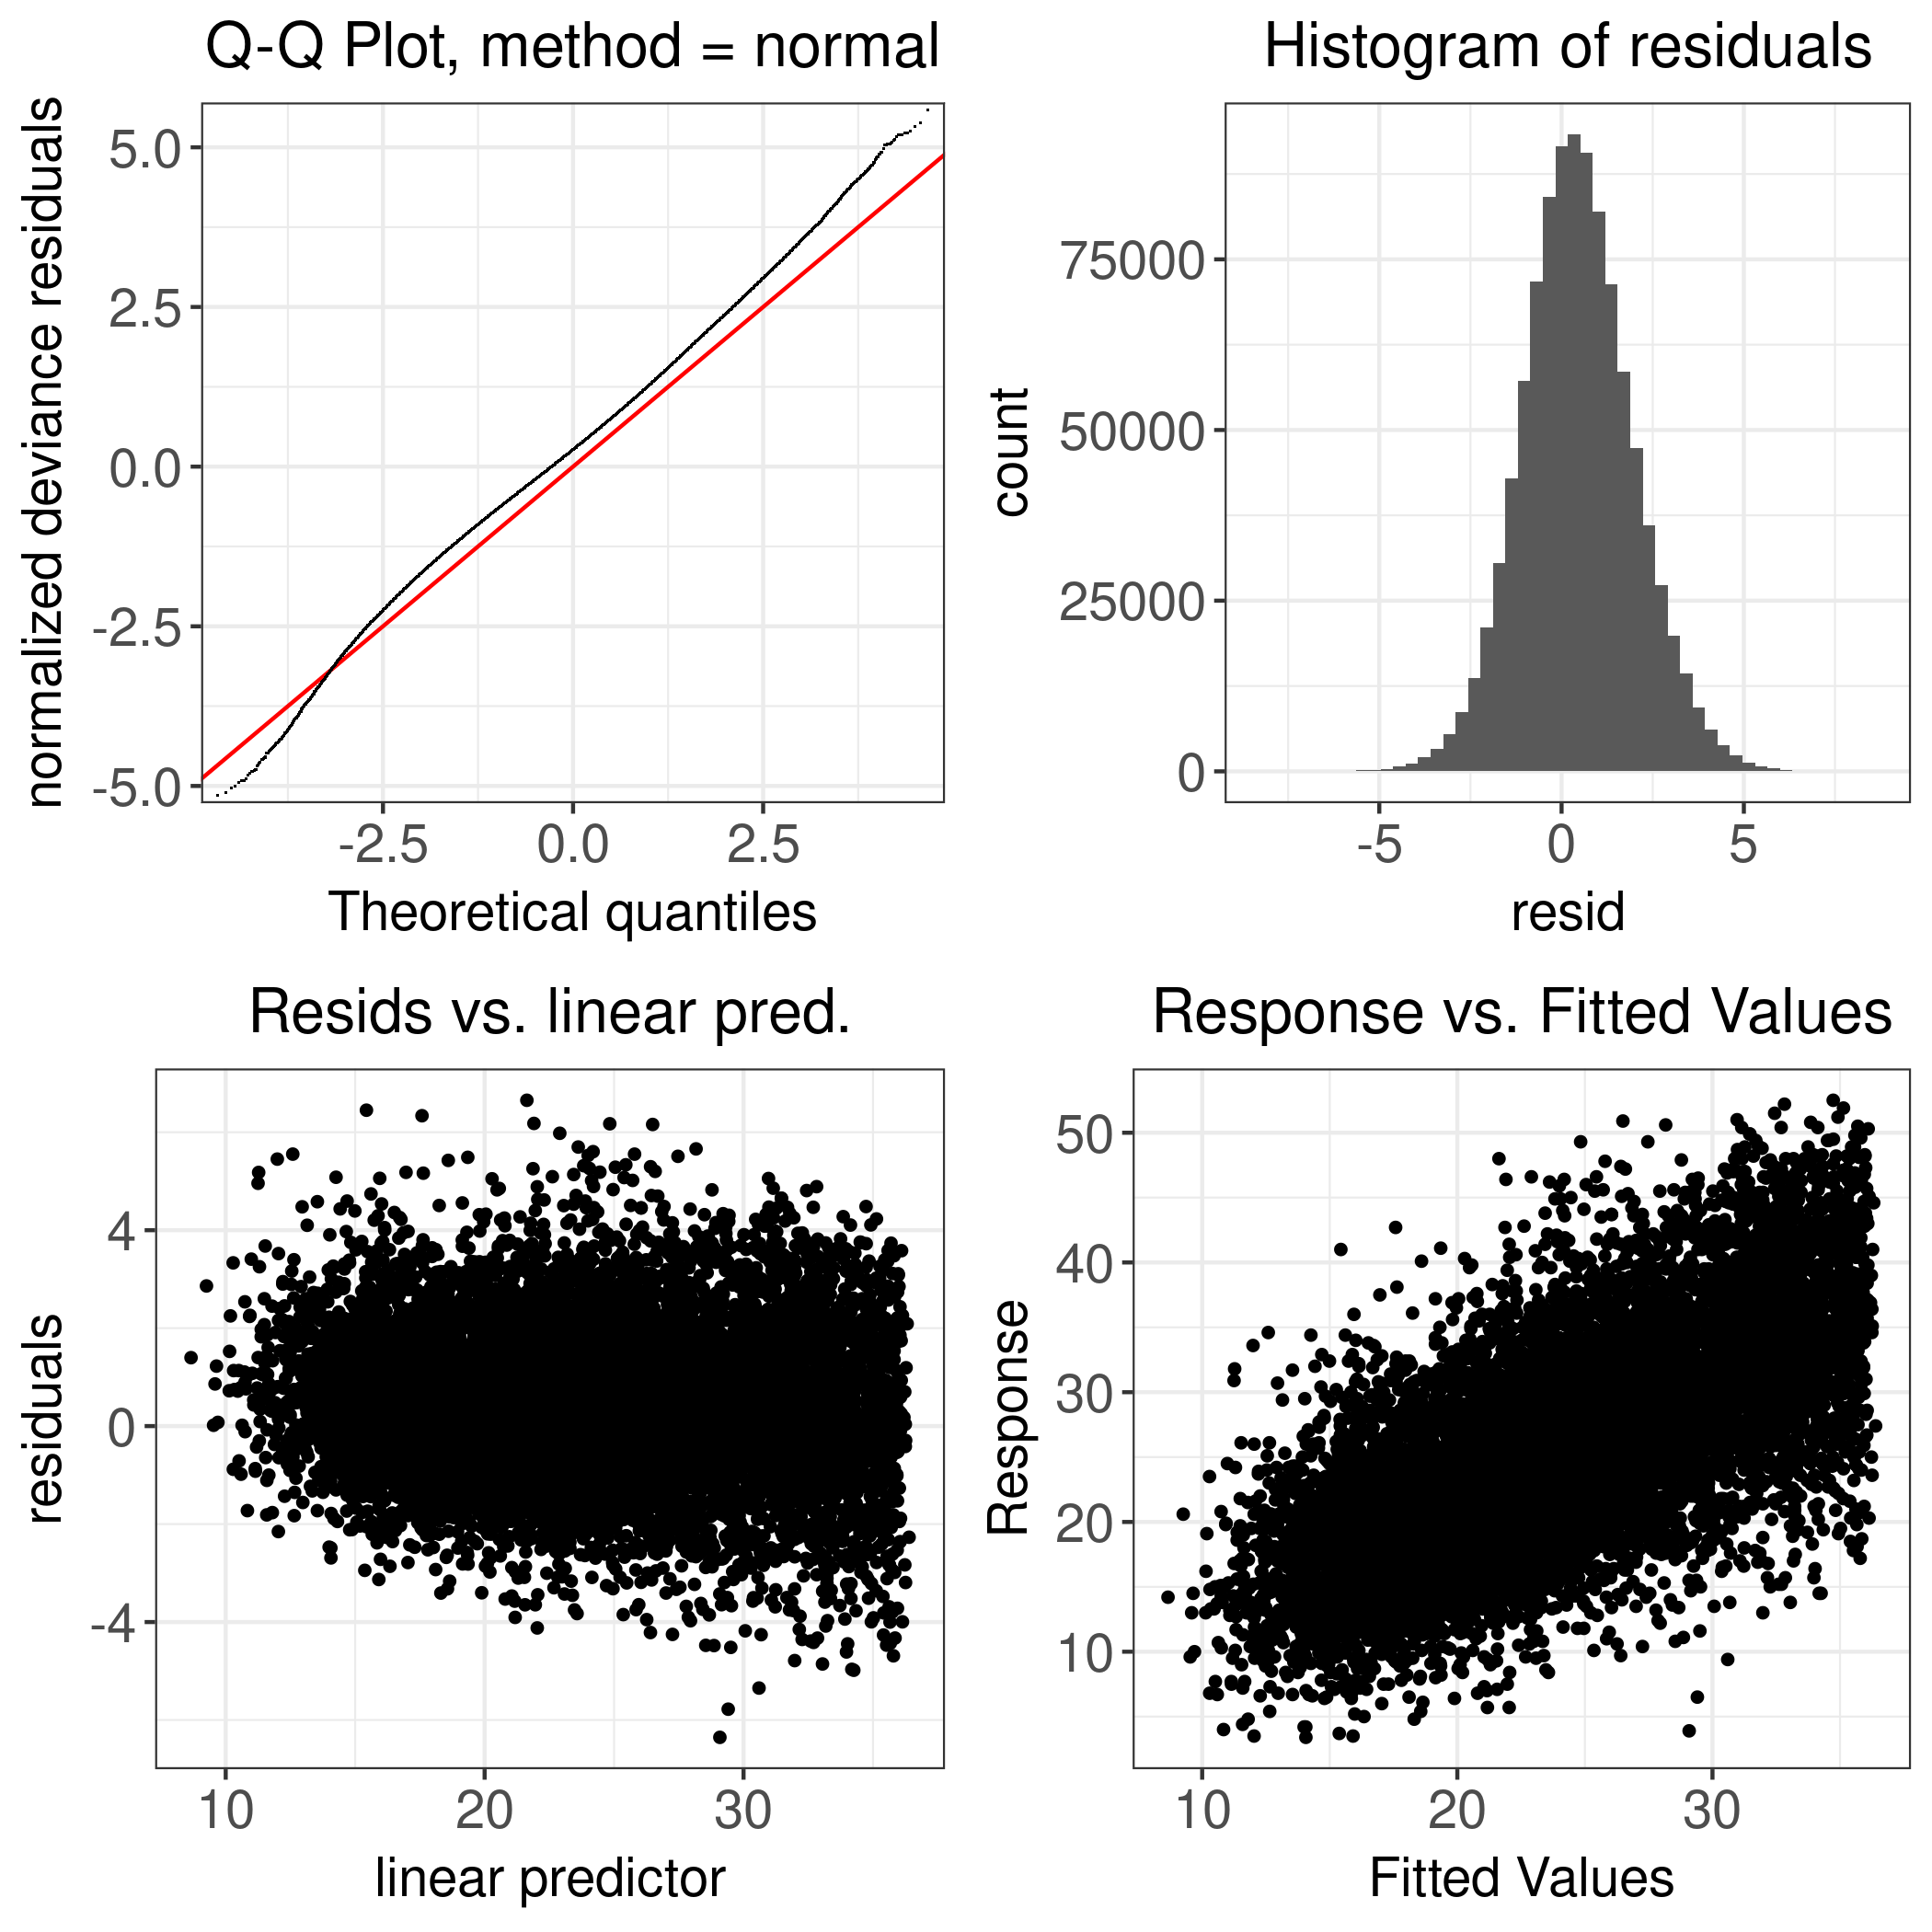
\includegraphics[width=0.6\textwidth]{thesis/figures/models/milk/after2010/ho_milk_after2010/ho_milk_after2010_diagnostics.png}
    \caption[]{Holstein: Milk Yield - 2011-2023 - Diagnostic Plot}
\end{figure}

\newpage
\paragraph{THI Effect and Lactation Curve} \quad \\
\begin{figure}[H]
    \centering
    \begin{subfigure}[b]{0.45\textwidth}
        \centering
        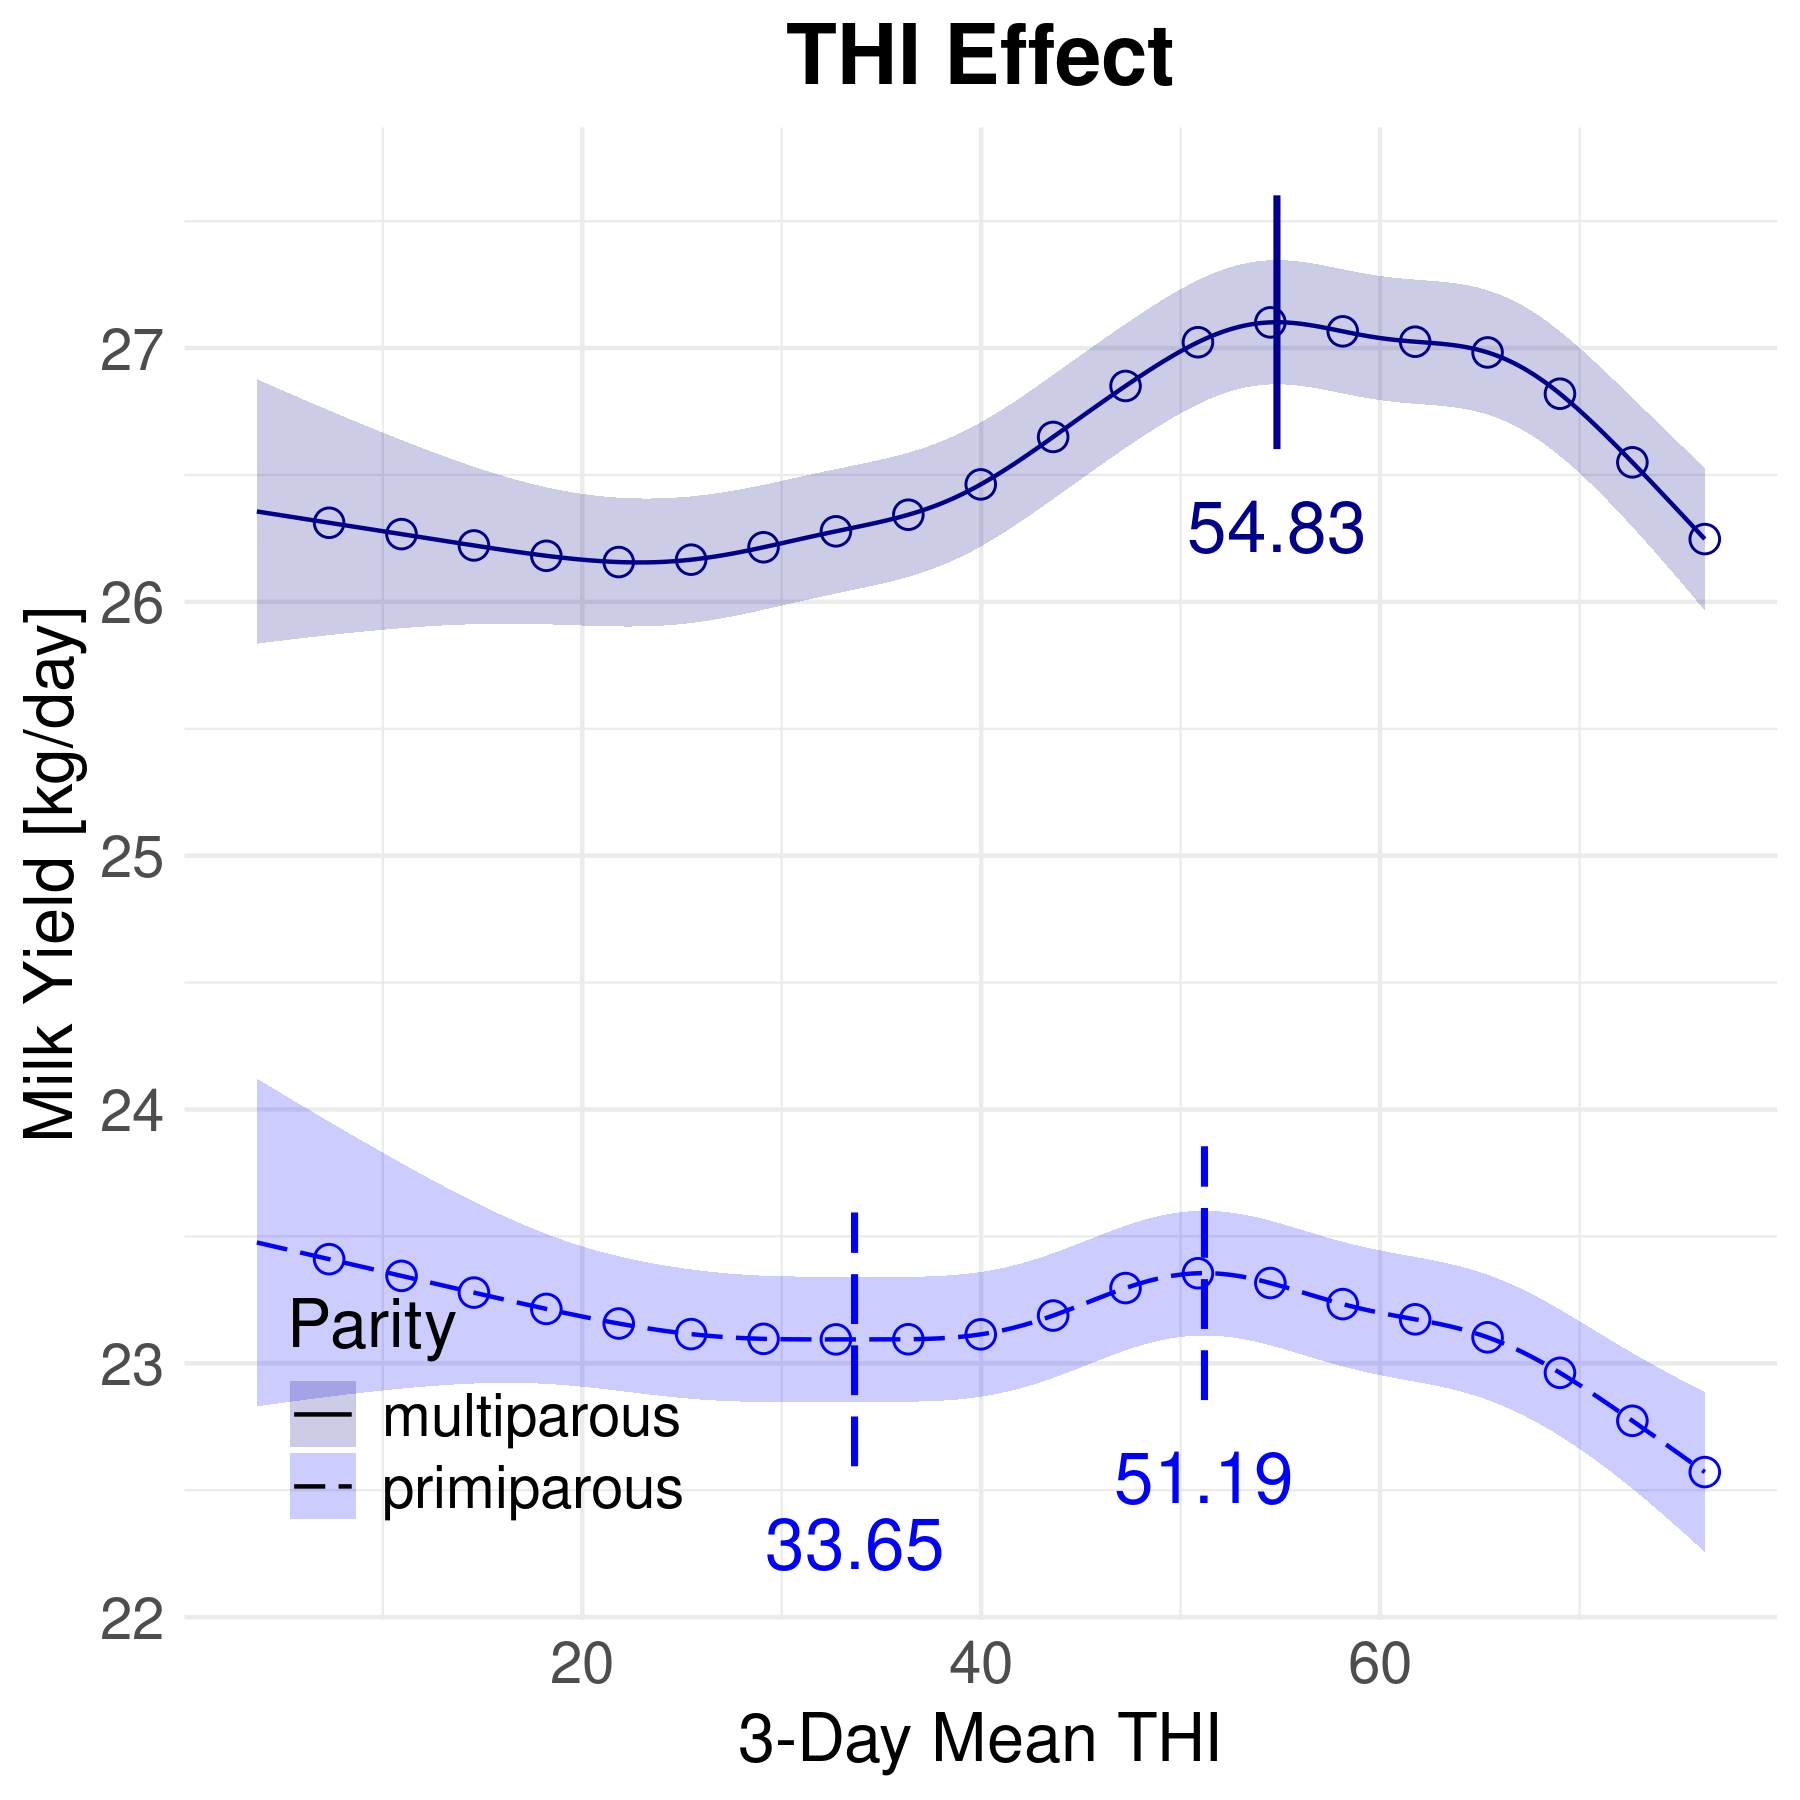
\includegraphics[width=\textwidth]{thesis/figures/models/milk/after2010/ho_milk_after2010/ho_milk_after2010_marginal_thi_milk_combined.png}
    \end{subfigure}
    \hspace{0.05\textwidth} % Optional space between the figures
    \begin{subfigure}[b]{0.45\textwidth}
        \centering
        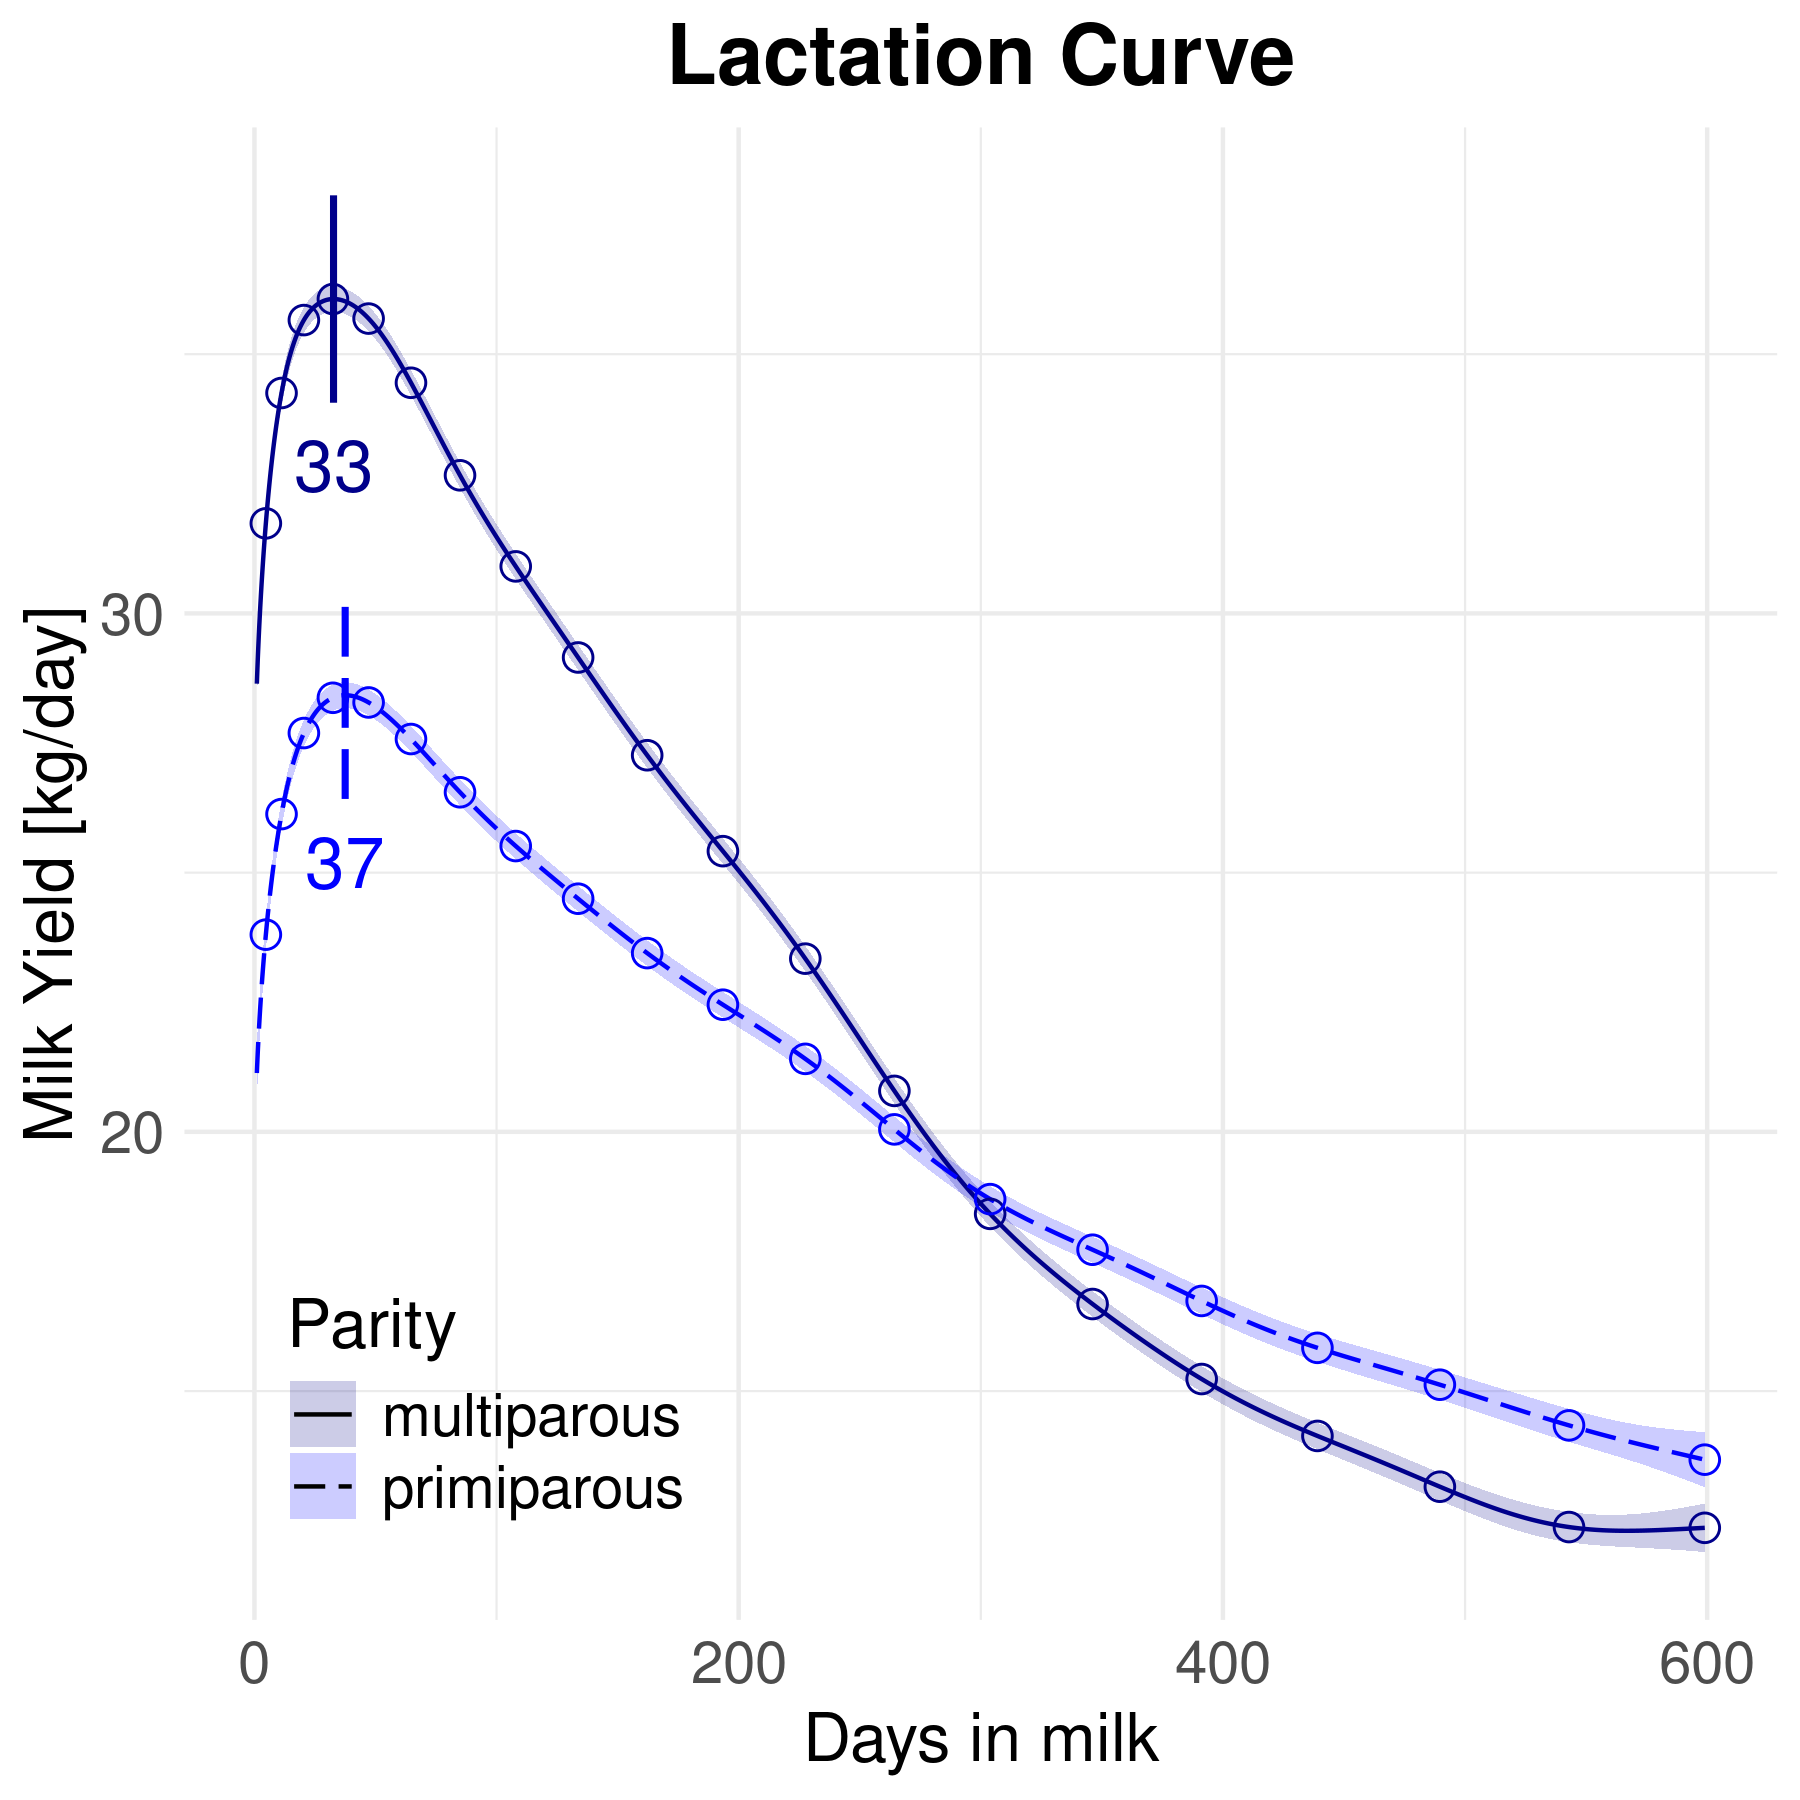
\includegraphics[width=\textwidth]{thesis/figures/models/milk/after2010/ho_milk_after2010/ho_milk_after2010_marginal_dim_milk_combined.png}
    \end{subfigure}
    \begin{subfigure}[b]{0.45\textwidth}
        \centering
        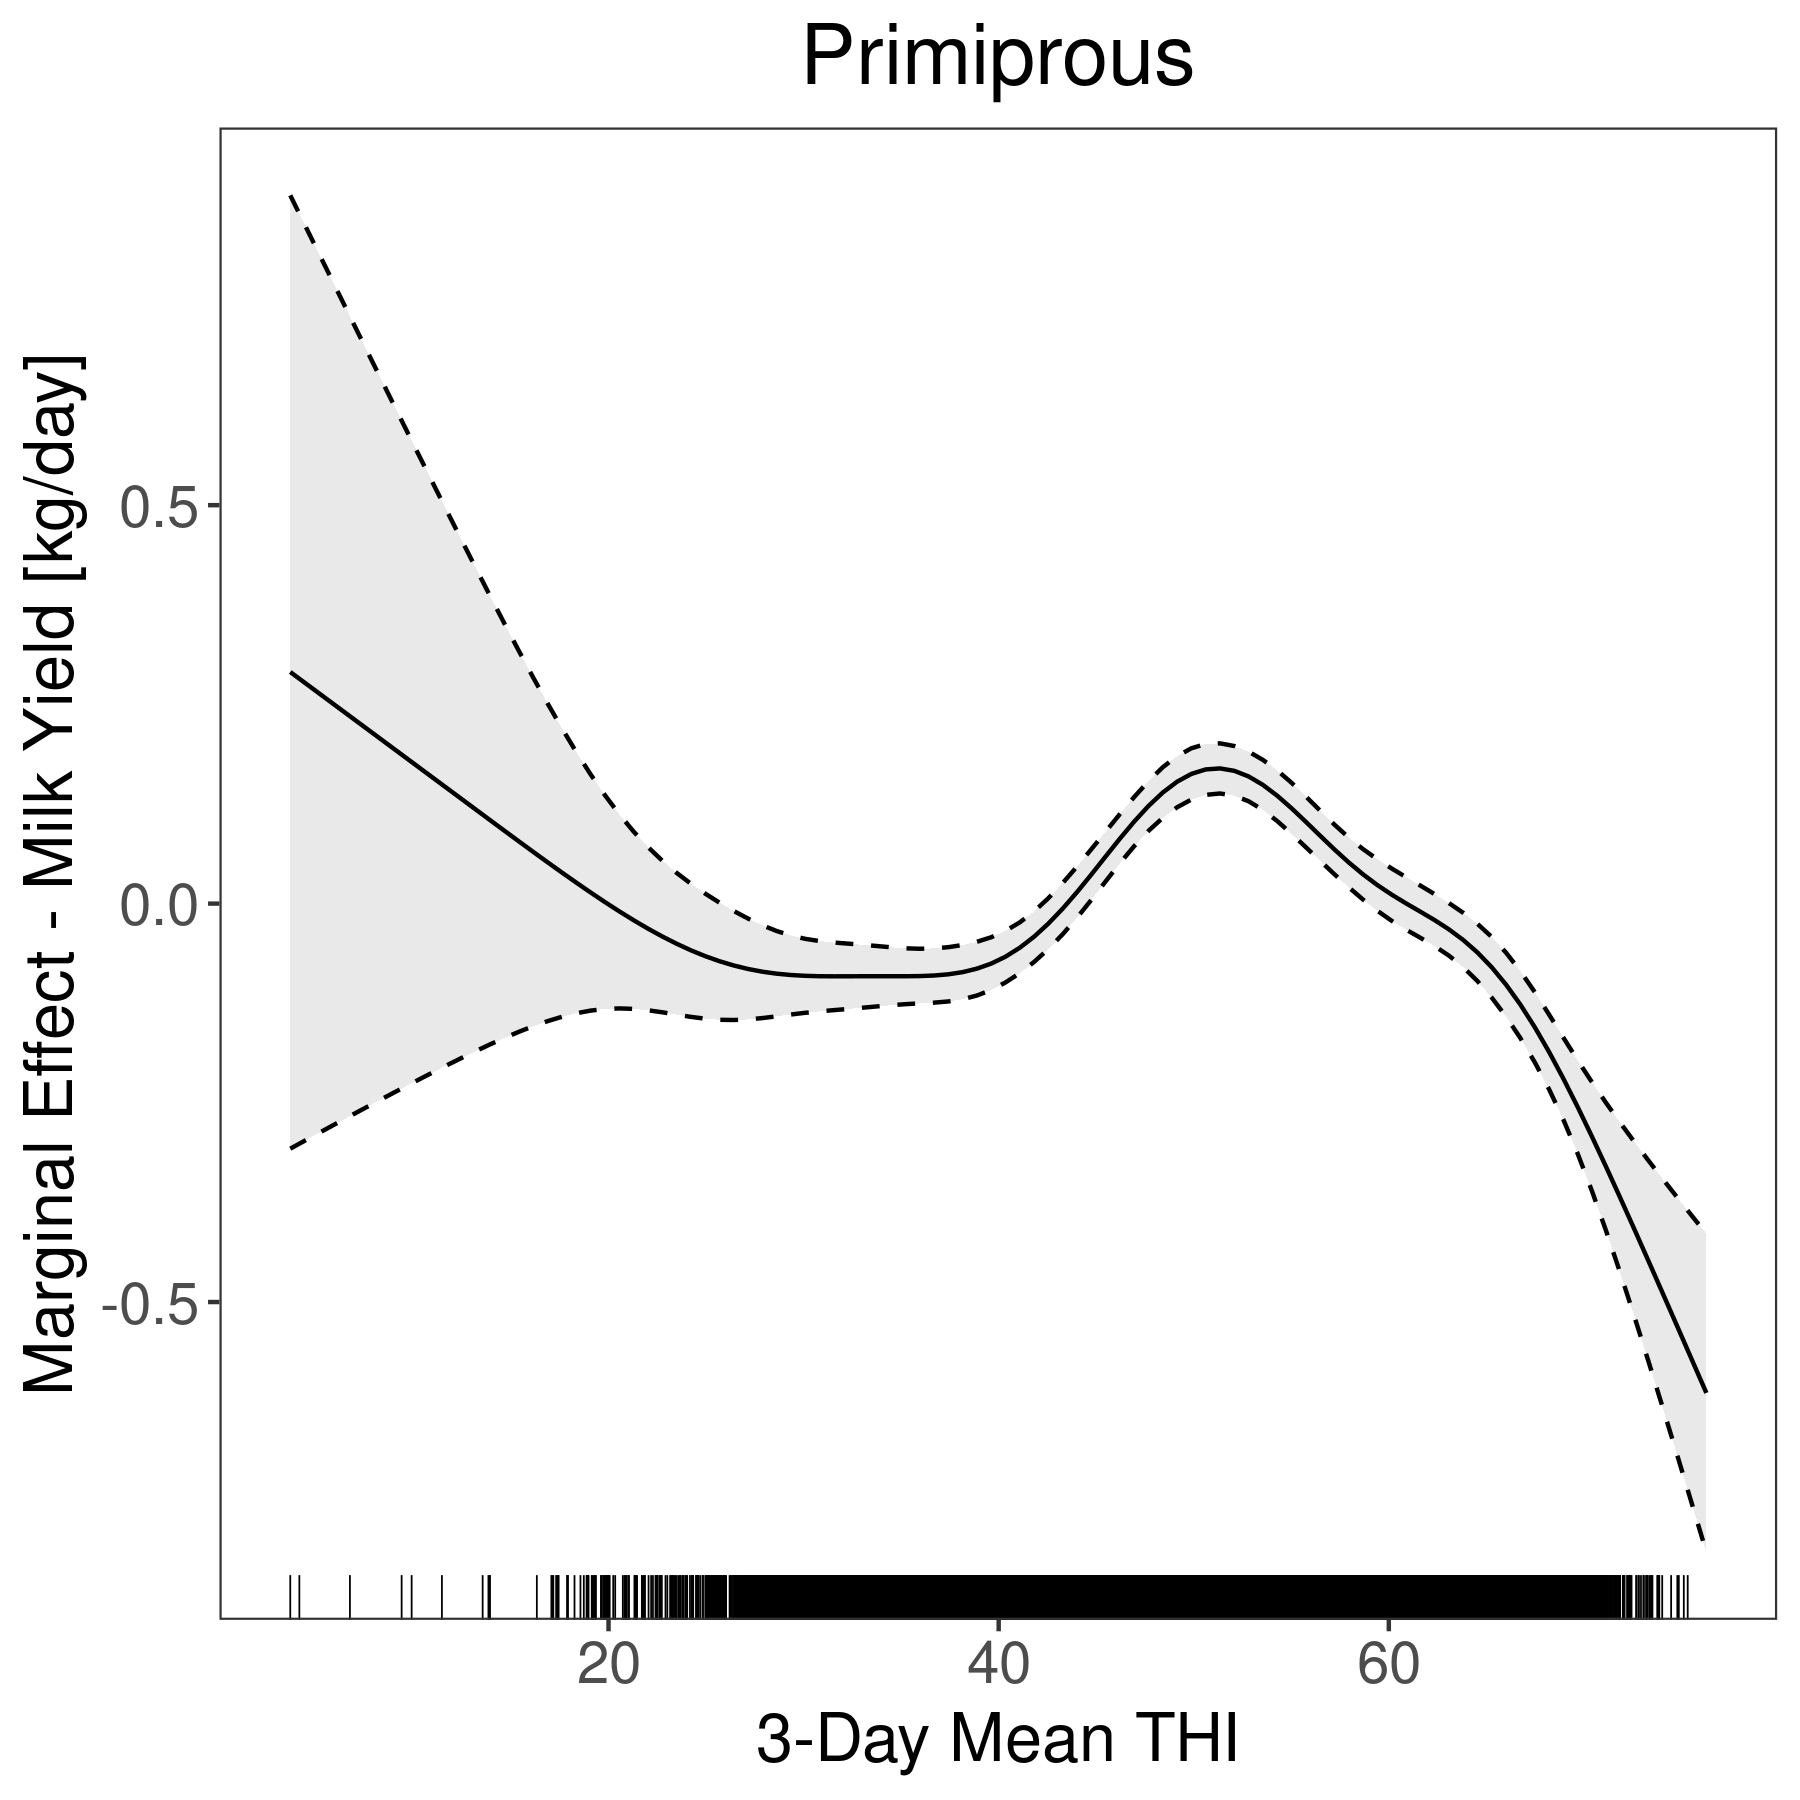
\includegraphics[width=\textwidth]{thesis/figures/models/milk/after2010/ho_milk_after2010/ho_milk_after2010_marginal_thi_milk_primi.png}
    \end{subfigure}
    \hspace{0.05\textwidth} % Optional space between the figures
    \begin{subfigure}[b]{0.45\textwidth}
        \centering
        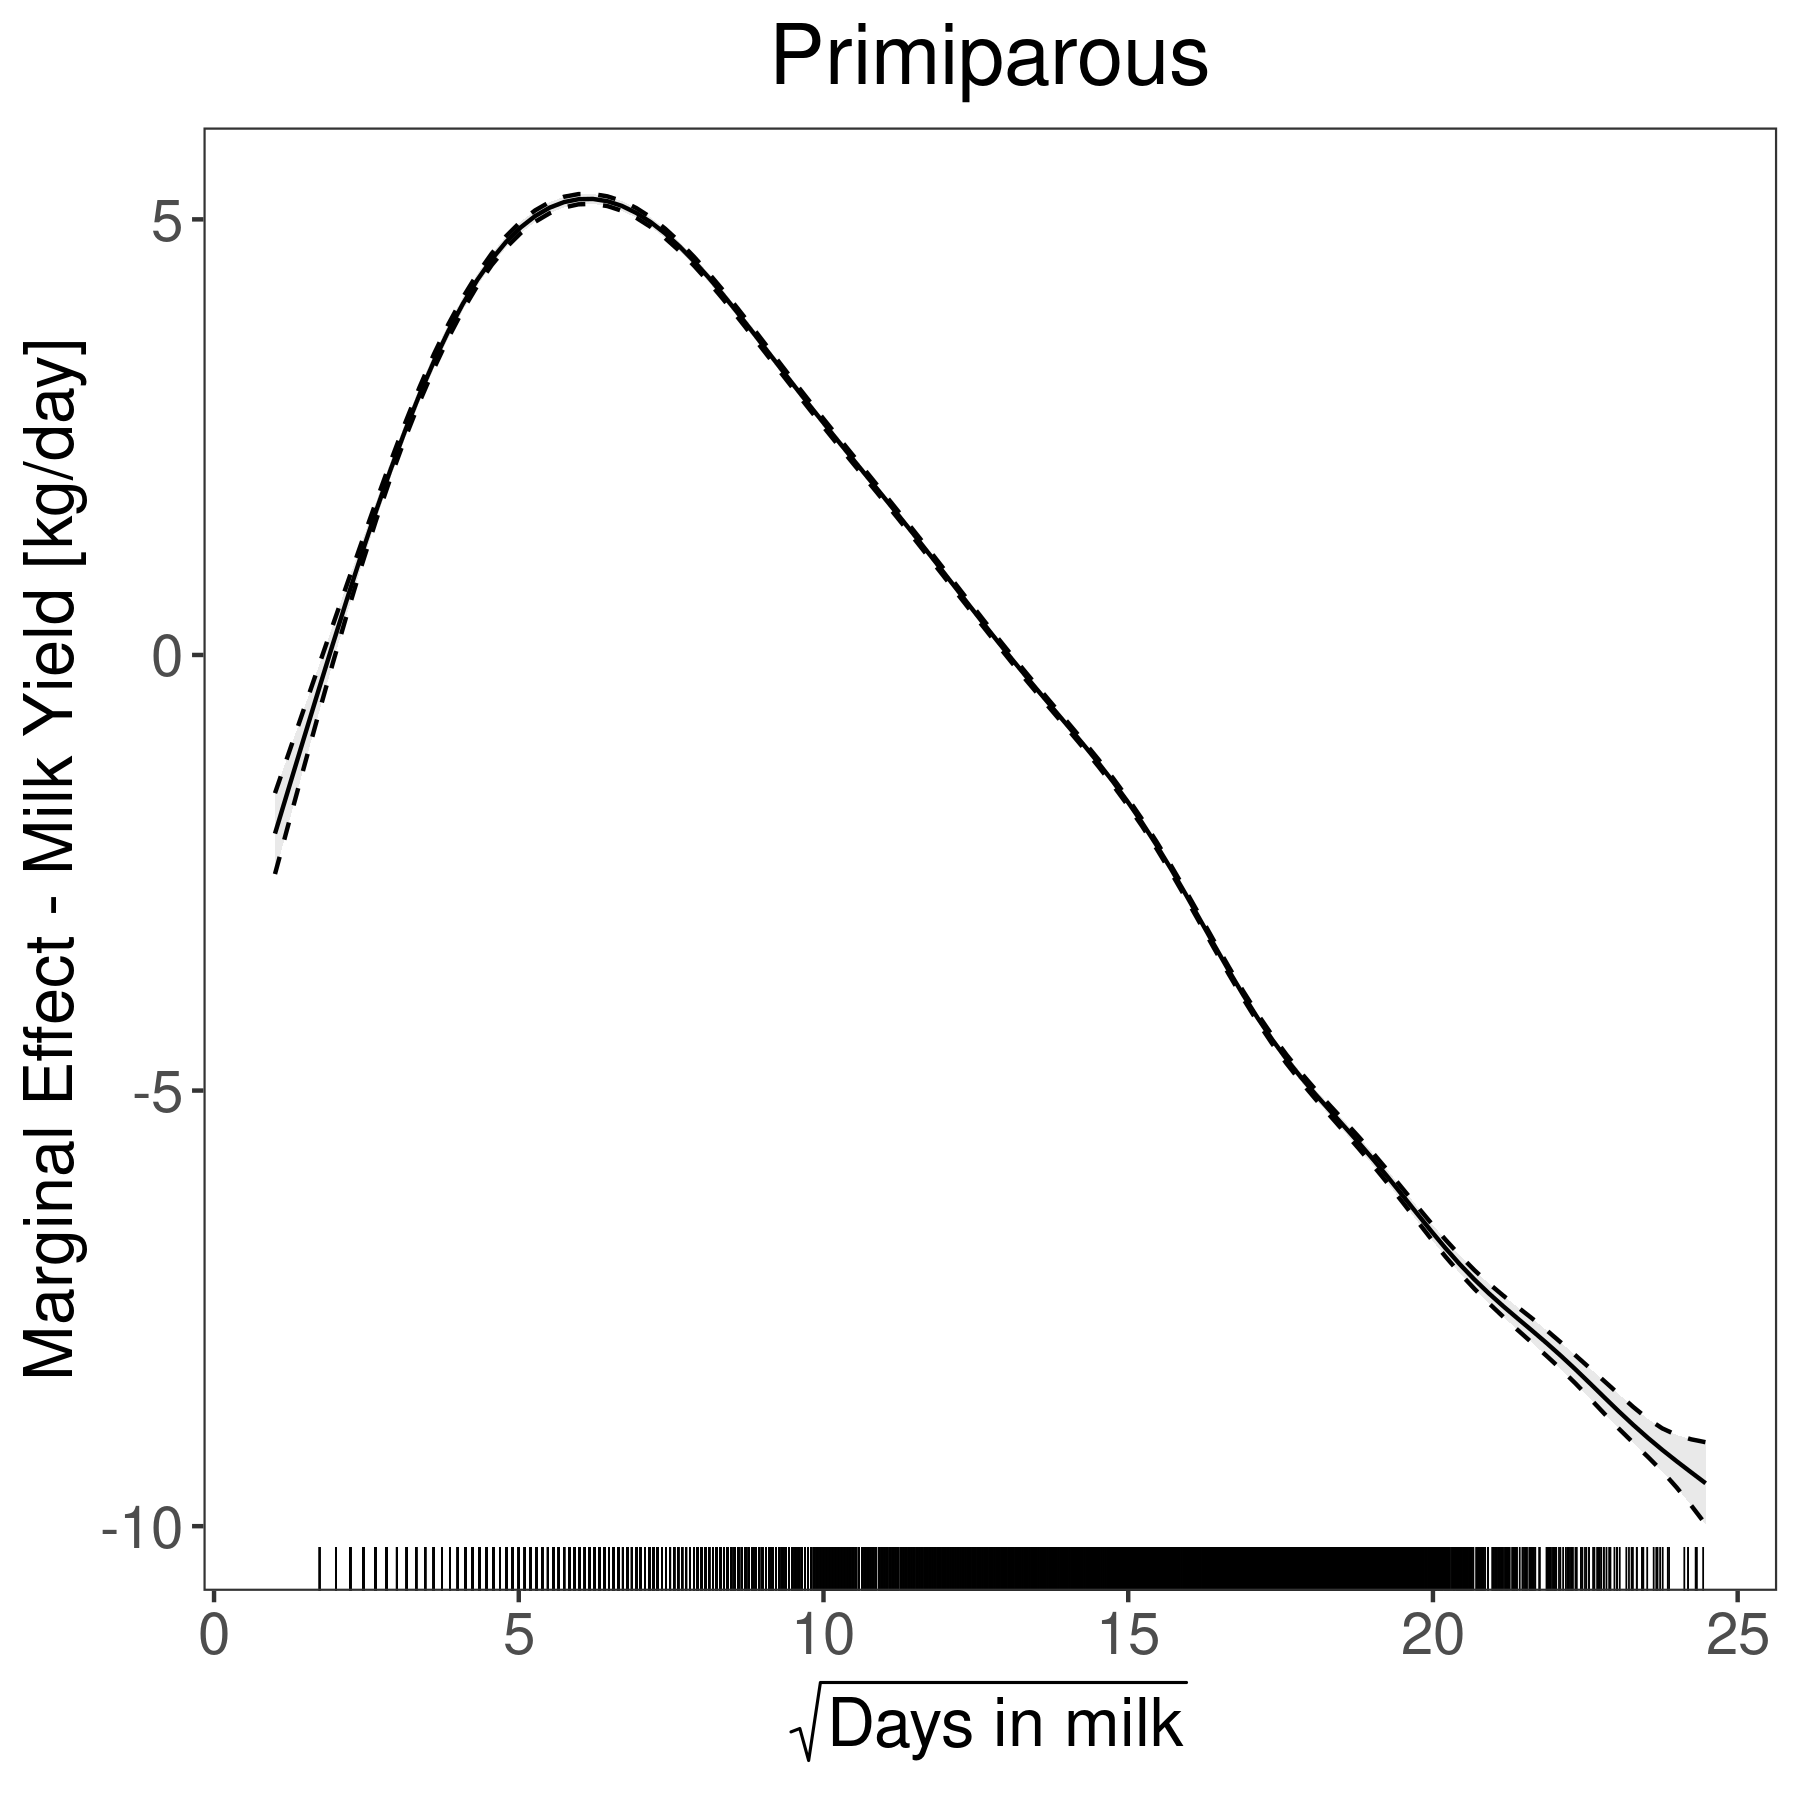
\includegraphics[width=\textwidth]{thesis/figures/models/milk/after2010/ho_milk_after2010/ho_milk_after2010_marginal_dim_milk_primi.png}
    \end{subfigure}
    \begin{subfigure}[b]{0.45\textwidth}
        \centering
        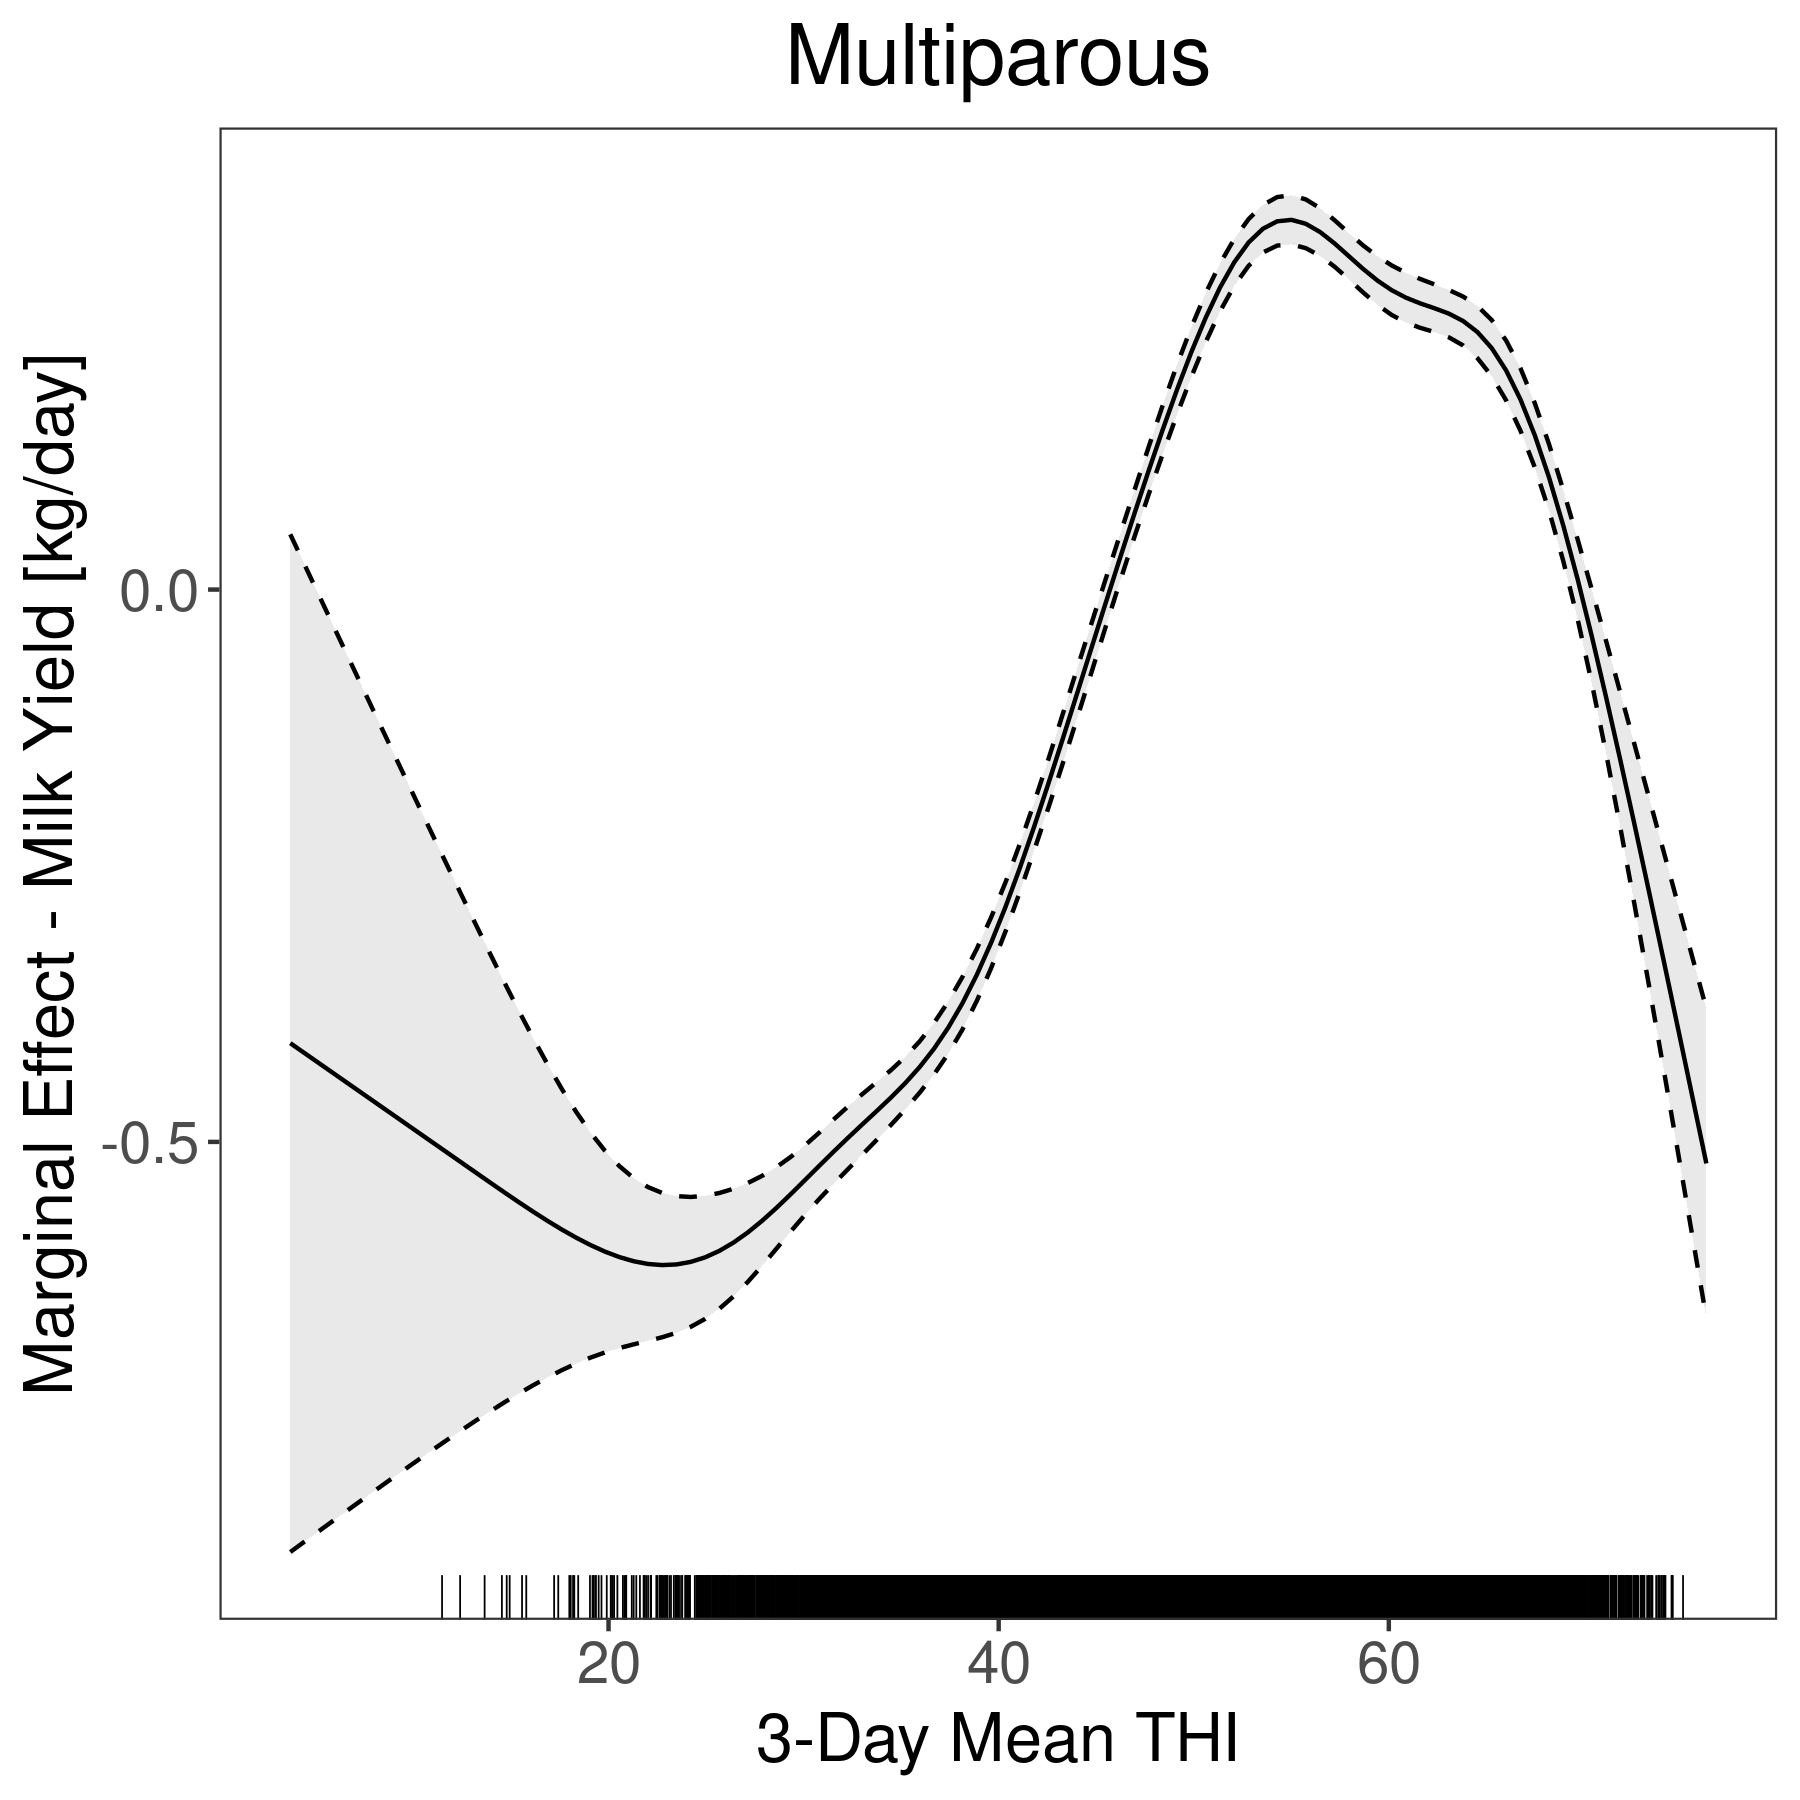
\includegraphics[width=\textwidth]{thesis/figures/models/milk/after2010/ho_milk_after2010/ho_milk_after2010_marginal_thi_milk_multi.png}
    \end{subfigure}
    \hspace{0.05\textwidth} % Optional space between the figures
    \begin{subfigure}[b]{0.45\textwidth}
        \centering
        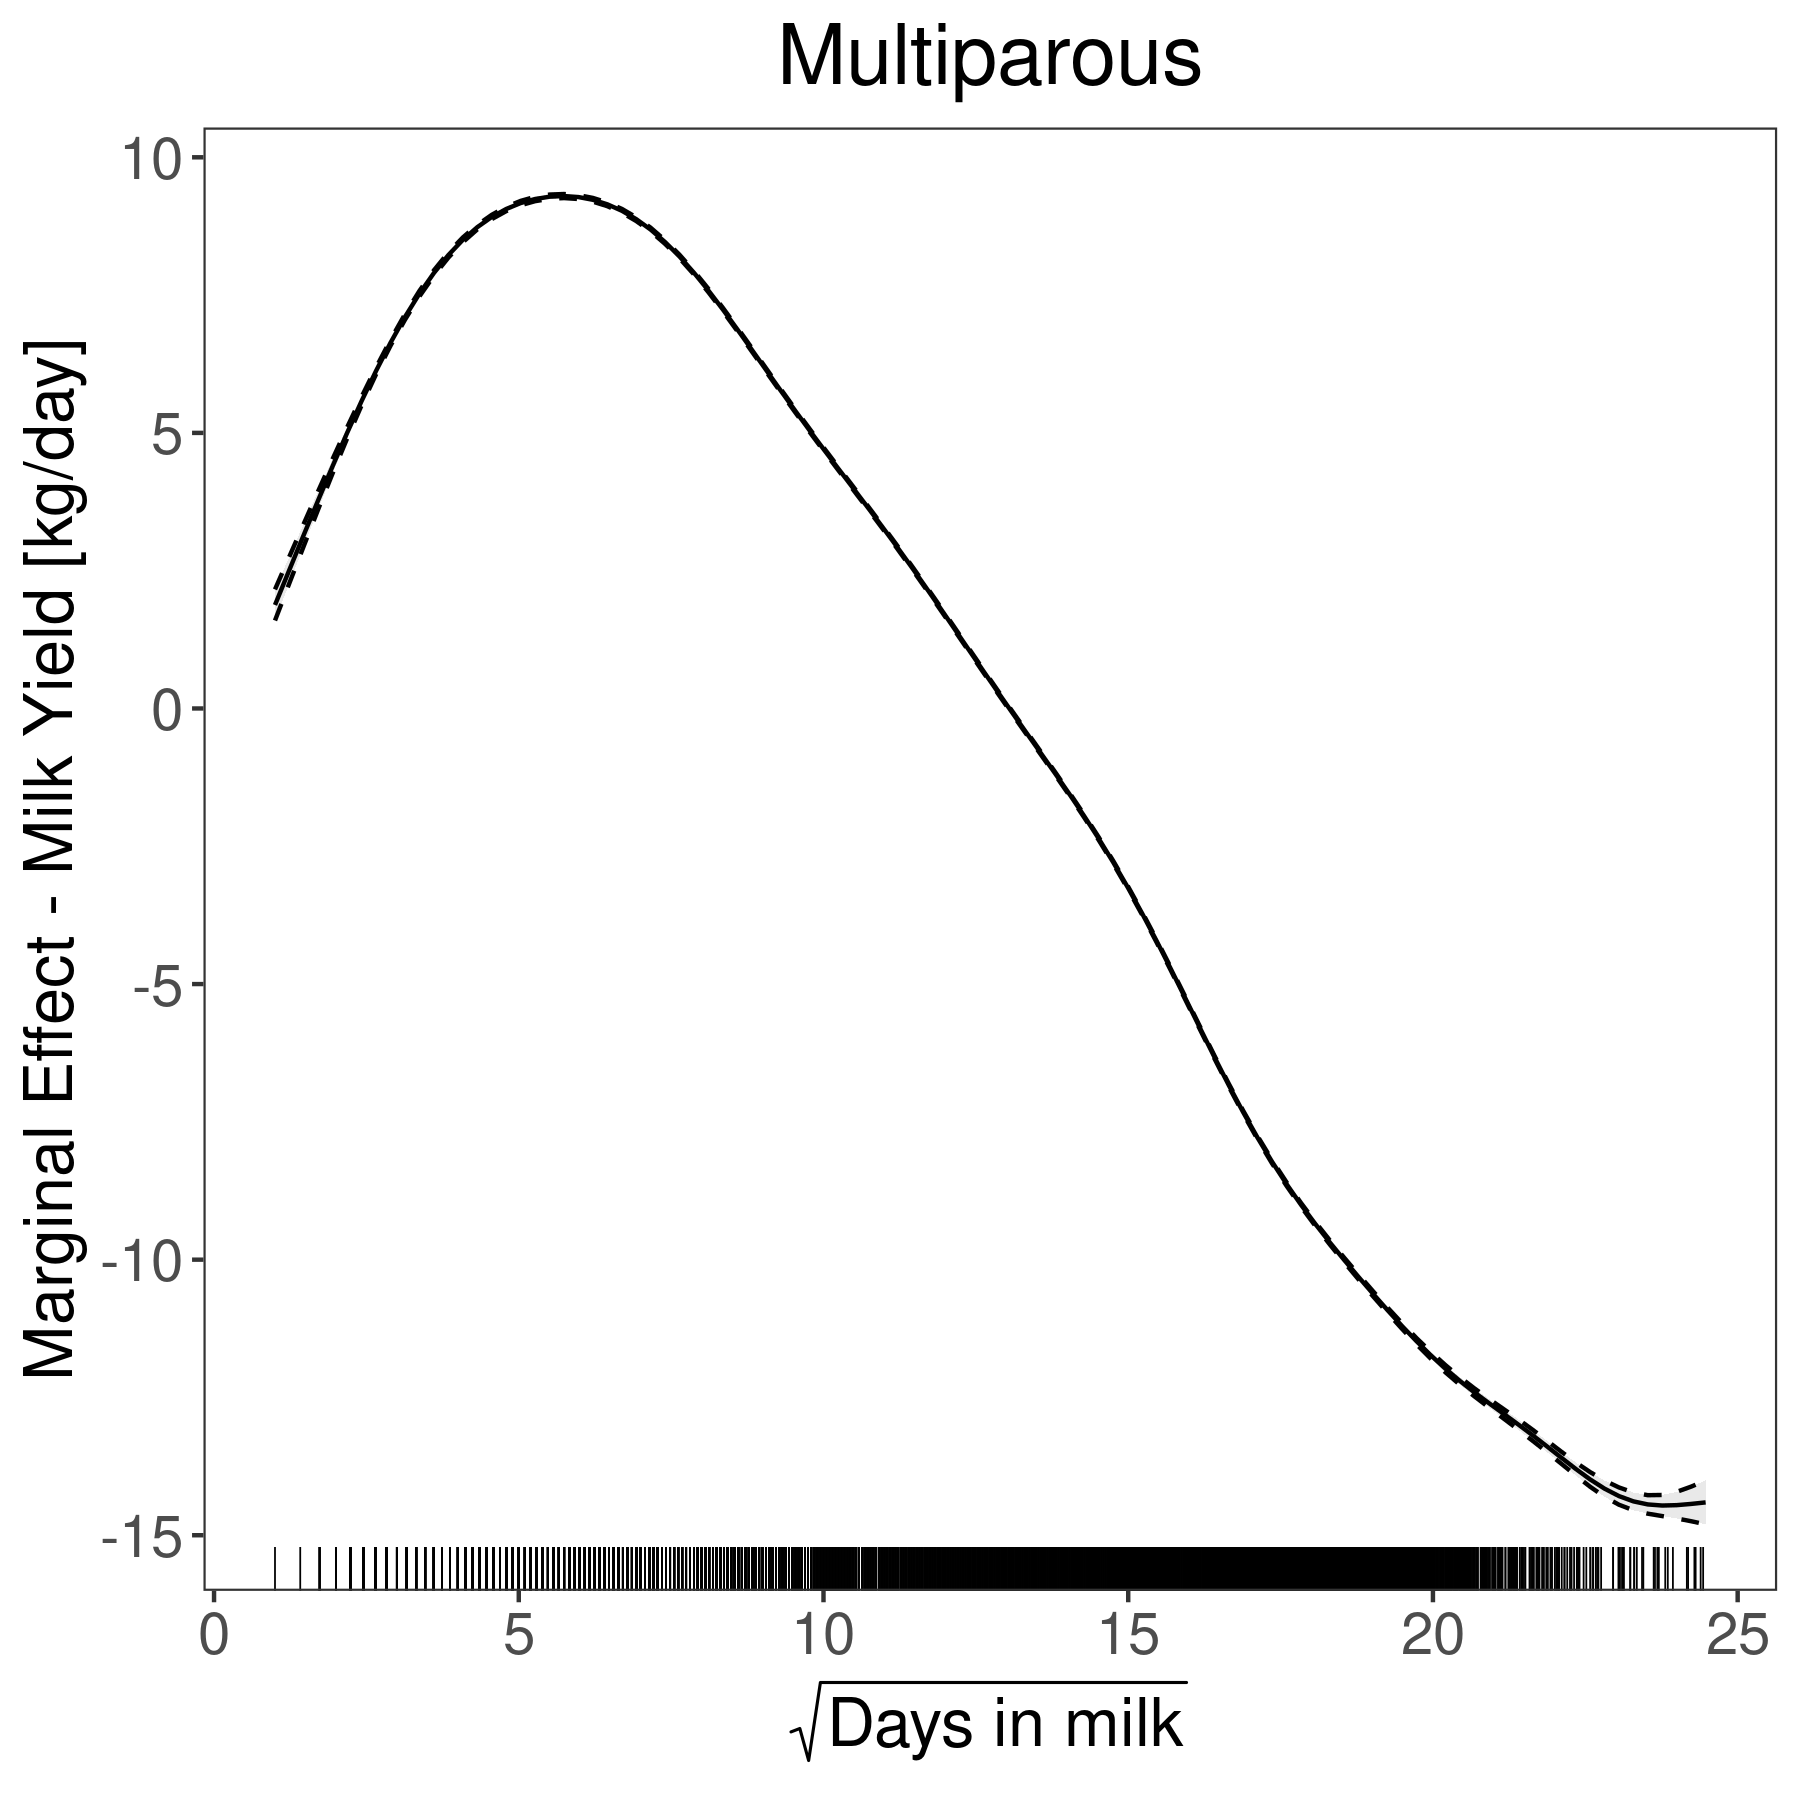
\includegraphics[width=\textwidth]{thesis/figures/models/milk/after2010/ho_milk_after2010/ho_milk_after2010_marginal_dim_milk_multi.png}
    \end{subfigure}
    \caption[]{Holstein: Milk Yield - 2010 - 2023 - THI Effect and Lactation Curve}
    \label{fig:main}
\end{figure}
\addtocontents{toc}{\protect\setcounter{tocdepth}{2}}

\section{Holstein: ECM Yield}
\subsection{Full Period: 1985-2023}\label{model:ho_ecm_full}
\paragraph{Model Summary} \quad \\

    \begin{table}[H]
    \centering
    \begin{tabular}{lrrrr}
    \textbf{A. parametric coefficients} & Estimate & Std. Error & t-value & p-value \\ 
       \hline
       \hline
  (Intercept) & 20.1076 & 0.1617 & 124.3358 & $<$ 0.0001 \\ 
  parityprimiparous & -3.9424 & 0.0093 & -422.7197 & $<$ 0.0001 \\ 
  year1986 & 0.1635 & 0.1304 & 1.2541 & 0.2098 \\ 
  year1987 & -0.1100 & 0.1299 & -0.8464 & 0.3973 \\ 
  year1988 & -0.4448 & 0.1288 & -3.4531 & 0.0006 \\ 
  year1989 & 0.1254 & 0.1278 & 0.9809 & 0.3267 \\ 
  year1990 & 0.5707 & 0.1281 & 4.4557 & $<$ 0.0001 \\ 
  year1991 & 0.7665 & 0.1268 & 6.0465 & $<$ 0.0001 \\ 
  year1992 & 1.1648 & 0.1260 & 9.2442 & $<$ 0.0001 \\ 
  year1993 & 1.2702 & 0.1250 & 10.1623 & $<$ 0.0001 \\ 
  year1994 & 0.9399 & 0.1233 & 7.6238 & $<$ 0.0001 \\ 
  year1995 & 1.3246 & 0.1236 & 10.7206 & $<$ 0.0001 \\ 
  year1996 & 1.7648 & 0.1222 & 14.4466 & $<$ 0.0001 \\ 
  year1997 & 2.3101 & 0.1223 & 18.8938 & $<$ 0.0001 \\ 
  year1998 & 2.9914 & 0.1206 & 24.8069 & $<$ 0.0001 \\ 
  year1999 & 2.6437 & 0.1193 & 22.1562 & $<$ 0.0001 \\ 
  year2000 & 2.5987 & 0.1186 & 21.9127 & $<$ 0.0001 \\ 
  year2001 & 2.9072 & 0.1179 & 24.6612 & $<$ 0.0001 \\ 
  year2002 & 3.0868 & 0.1175 & 26.2770 & $<$ 0.0001 \\ 
  year2003 & 3.5531 & 0.1171 & 30.3539 & $<$ 0.0001 \\ 
  year2004 & 4.0984 & 0.1169 & 35.0471 & $<$ 0.0001 \\ 
  year2005 & 4.7114 & 0.1167 & 40.3673 & $<$ 0.0001 \\ 
  year2006 & 4.6636 & 0.1166 & 39.9990 & $<$ 0.0001 \\ 
  year2007 & 4.3704 & 0.1165 & 37.5094 & $<$ 0.0001 \\ 
  year2008 & 4.7638 & 0.1164 & 40.9126 & $<$ 0.0001 \\ 
  year2009 & 5.1818 & 0.1165 & 44.4952 & $<$ 0.0001 \\ 
  year2010 & 5.8336 & 0.1164 & 50.1183 & $<$ 0.0001 \\ 
  year2011 & 6.0286 & 0.1164 & 51.7791 & $<$ 0.0001 \\ 
  year2012 & 6.1847 & 0.1167 & 53.0014 & $<$ 0.0001 \\ 
  year2013 & 5.7015 & 0.1168 & 48.8341 & $<$ 0.0001 \\ 
  year2014 & 6.3304 & 0.1167 & 54.2257 & $<$ 0.0001 \\ 
  year2015 & 6.7851 & 0.1168 & 58.0841 & $<$ 0.0001 \\ 
  year2016 & 7.3041 & 0.1170 & 62.4072 & $<$ 0.0001 \\ 
  year2017 & 7.3981 & 0.1169 & 63.2676 & $<$ 0.0001 \\ 
  year2018 & 8.0557 & 0.1171 & 68.8206 & $<$ 0.0001 \\ 
  year2019 & 8.2896 & 0.1171 & 70.8058 & $<$ 0.0001 \\ 
  year2020 & 8.9829 & 0.1174 & 76.5305 & $<$ 0.0001 \\ 
  year2021 & 9.5582 & 0.1170 & 81.6686 & $<$ 0.0001 \\ 
  year2022 & 9.6665 & 0.1169 & 82.6636 & $<$ 0.0001 \\ 
  year2023 & 10.4348 & 0.1167 & 89.4257 & $<$ 0.0001 \\ 
       \hline
    \textbf{B. smooth terms} & edf & Ref.df & F-value & p-value \\ 
    \hline
    \hline
  s(thi\_mean\_t0\_3d):paritymultiparous & 8.2862 & 8.2862 & 226.9355 & $<$ 0.0001 \\ 
  s(thi\_mean\_t0\_3d):parityprimiparous & 6.8141 & 6.8141 & 229.3868 & $<$ 0.0001 \\ 
  s(days\_in\_milk\_t):paritymultiparous & 13.5893 & 13.5893 & 104352.5853 & $<$ 0.0001 \\ 
  s(days\_in\_milk\_t):parityprimiparous & 12.9465 & 12.9465 & 10972.7975 & $<$ 0.0001 \\
       \hline
    \end{tabular}
    \caption[]{Holstein: ECM Yield - 1985-2023 - GAMM model summary without random effect terms.}
    \end{table}

\newpage
\begin{table}[H]
\centering
\begin{tabular}
{l | r | r | r | r}
\textbf{Smooth Term Fixed Effect} & Est. & SE & z & p\\
\hline
\hline
s(thi\_mean\_t0\_3d):multiFx1 & 0.638531  &  0.115151   & 5.55 &  $<$ 1e-07 \\
s(thi\_mean\_t0\_3d):primiFx1 & 0.559616  &  0.129725   &  4.31  &  $<$ 1e-04\\
s(days\_in\_milk\_):multiFx1 &  1.239    & 0.456686 &   2.71  &  0.0067\\
s(days\_in\_milk\_):primiFx1 & 2.33168  &   0.535407  &   4.35  &  $<$ 1e-04\\
\hline
\textbf{Variance Component} & Estimated $\sigma$ & & & \\
\hline
\hline
$\sigma_\alpha$ & 3.11752 & &  & \\
$\sigma_\iota$ & 1.07133 & & & \\
$\sigma_\phi$ & 3.47683 & & & \\
s(thi\_mean\_t0\_3d):multi & 2.15566 & & & \\
s(days\_in\_milk\_):primi & 6.54541 & & & \\
s(days\_in\_milk\_):multi & 8.73852 & & & \\
s(thi\_mean\_t0\_3d):primi & 1.38212 & & & \\
Residual & 4.16782 & & & \\
\end{tabular}
\caption[]{Holstein: ECM Yield - 1985-2023 - Mixed Model Summary - Smooth Terms and Random Effects.}
\end{table}



\paragraph{Model Diagnostics} \quad \\
\begin{figure}[H]
    \centering
    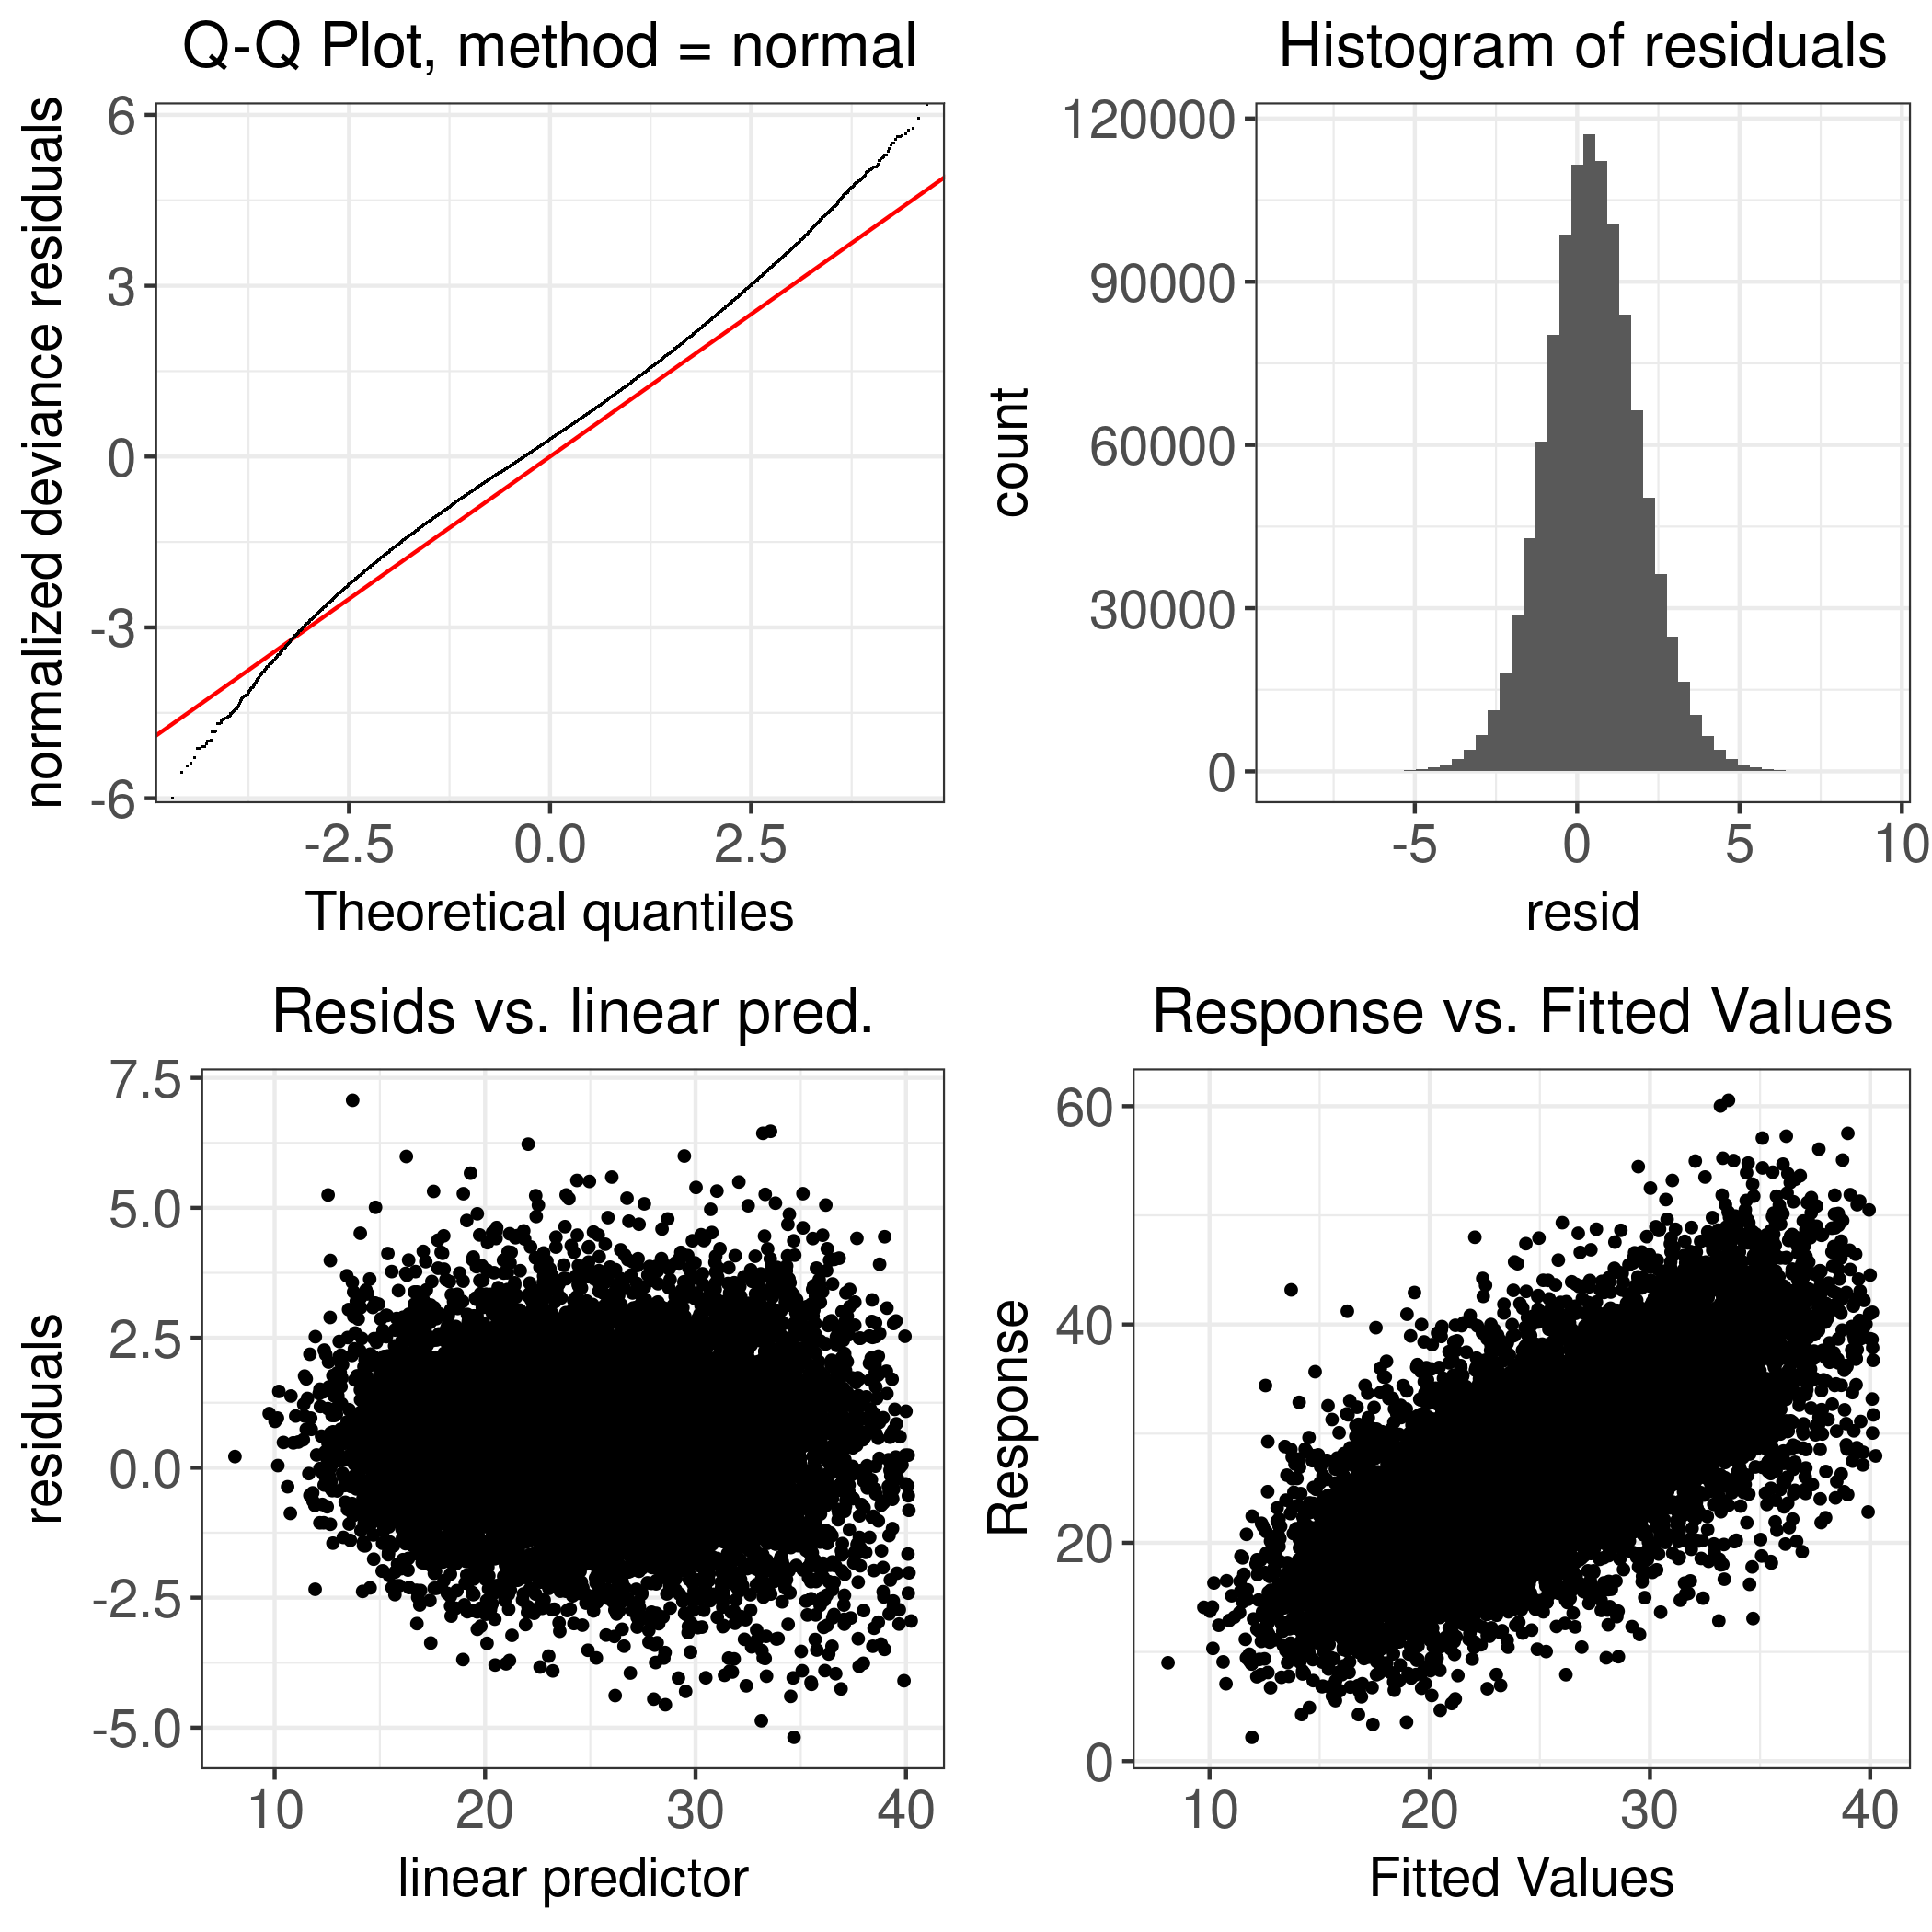
\includegraphics[width=0.6\textwidth]{thesis/figures/models/ecm/full/ho_ecm_full/ho_ecm_full_diagnostics.png}
    \caption[]{Holstein: ECM Yield - 1985-2023 - Diagnostic Plot}
\end{figure}

\newpage
\paragraph{THI Effect and Lactation Curve} \quad \\
\begin{figure}[H]
    \centering
    \begin{subfigure}[b]{0.45\textwidth}
        \centering
        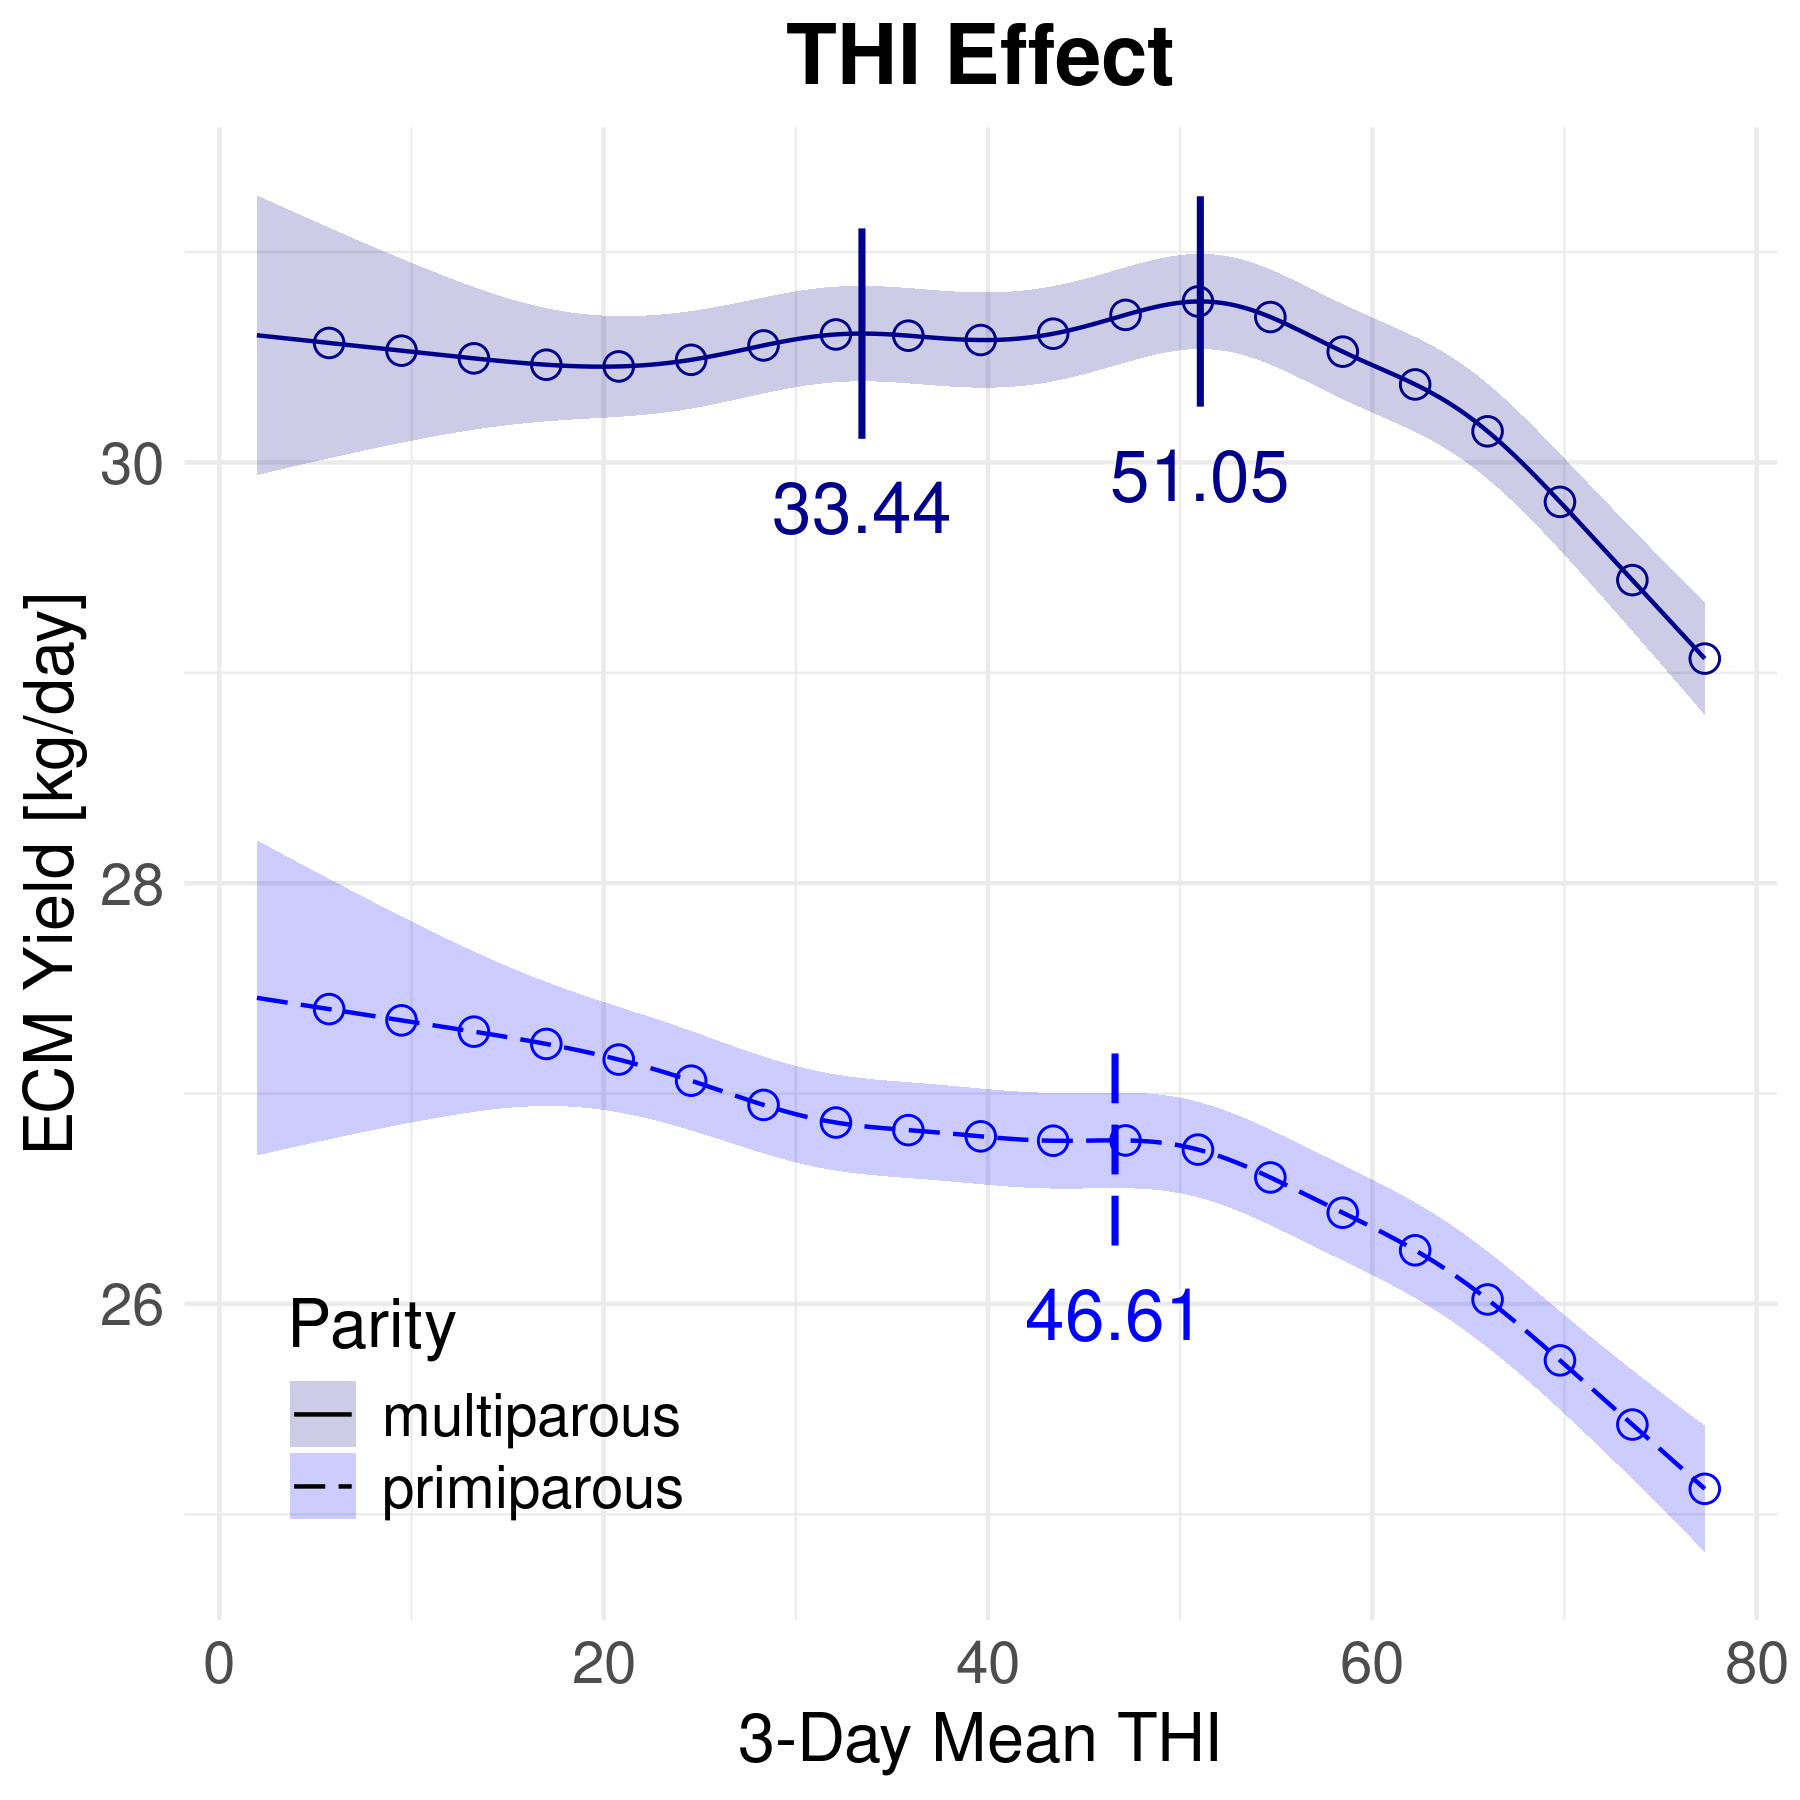
\includegraphics[width=\textwidth]{thesis/figures/models/ecm/full/ho_ecm_full/ho_ecm_full_marginal_thi_milk_combined.png}
    \end{subfigure}
    \hspace{0.05\textwidth} % Optional space between the figures
    \begin{subfigure}[b]{0.45\textwidth}
        \centering
        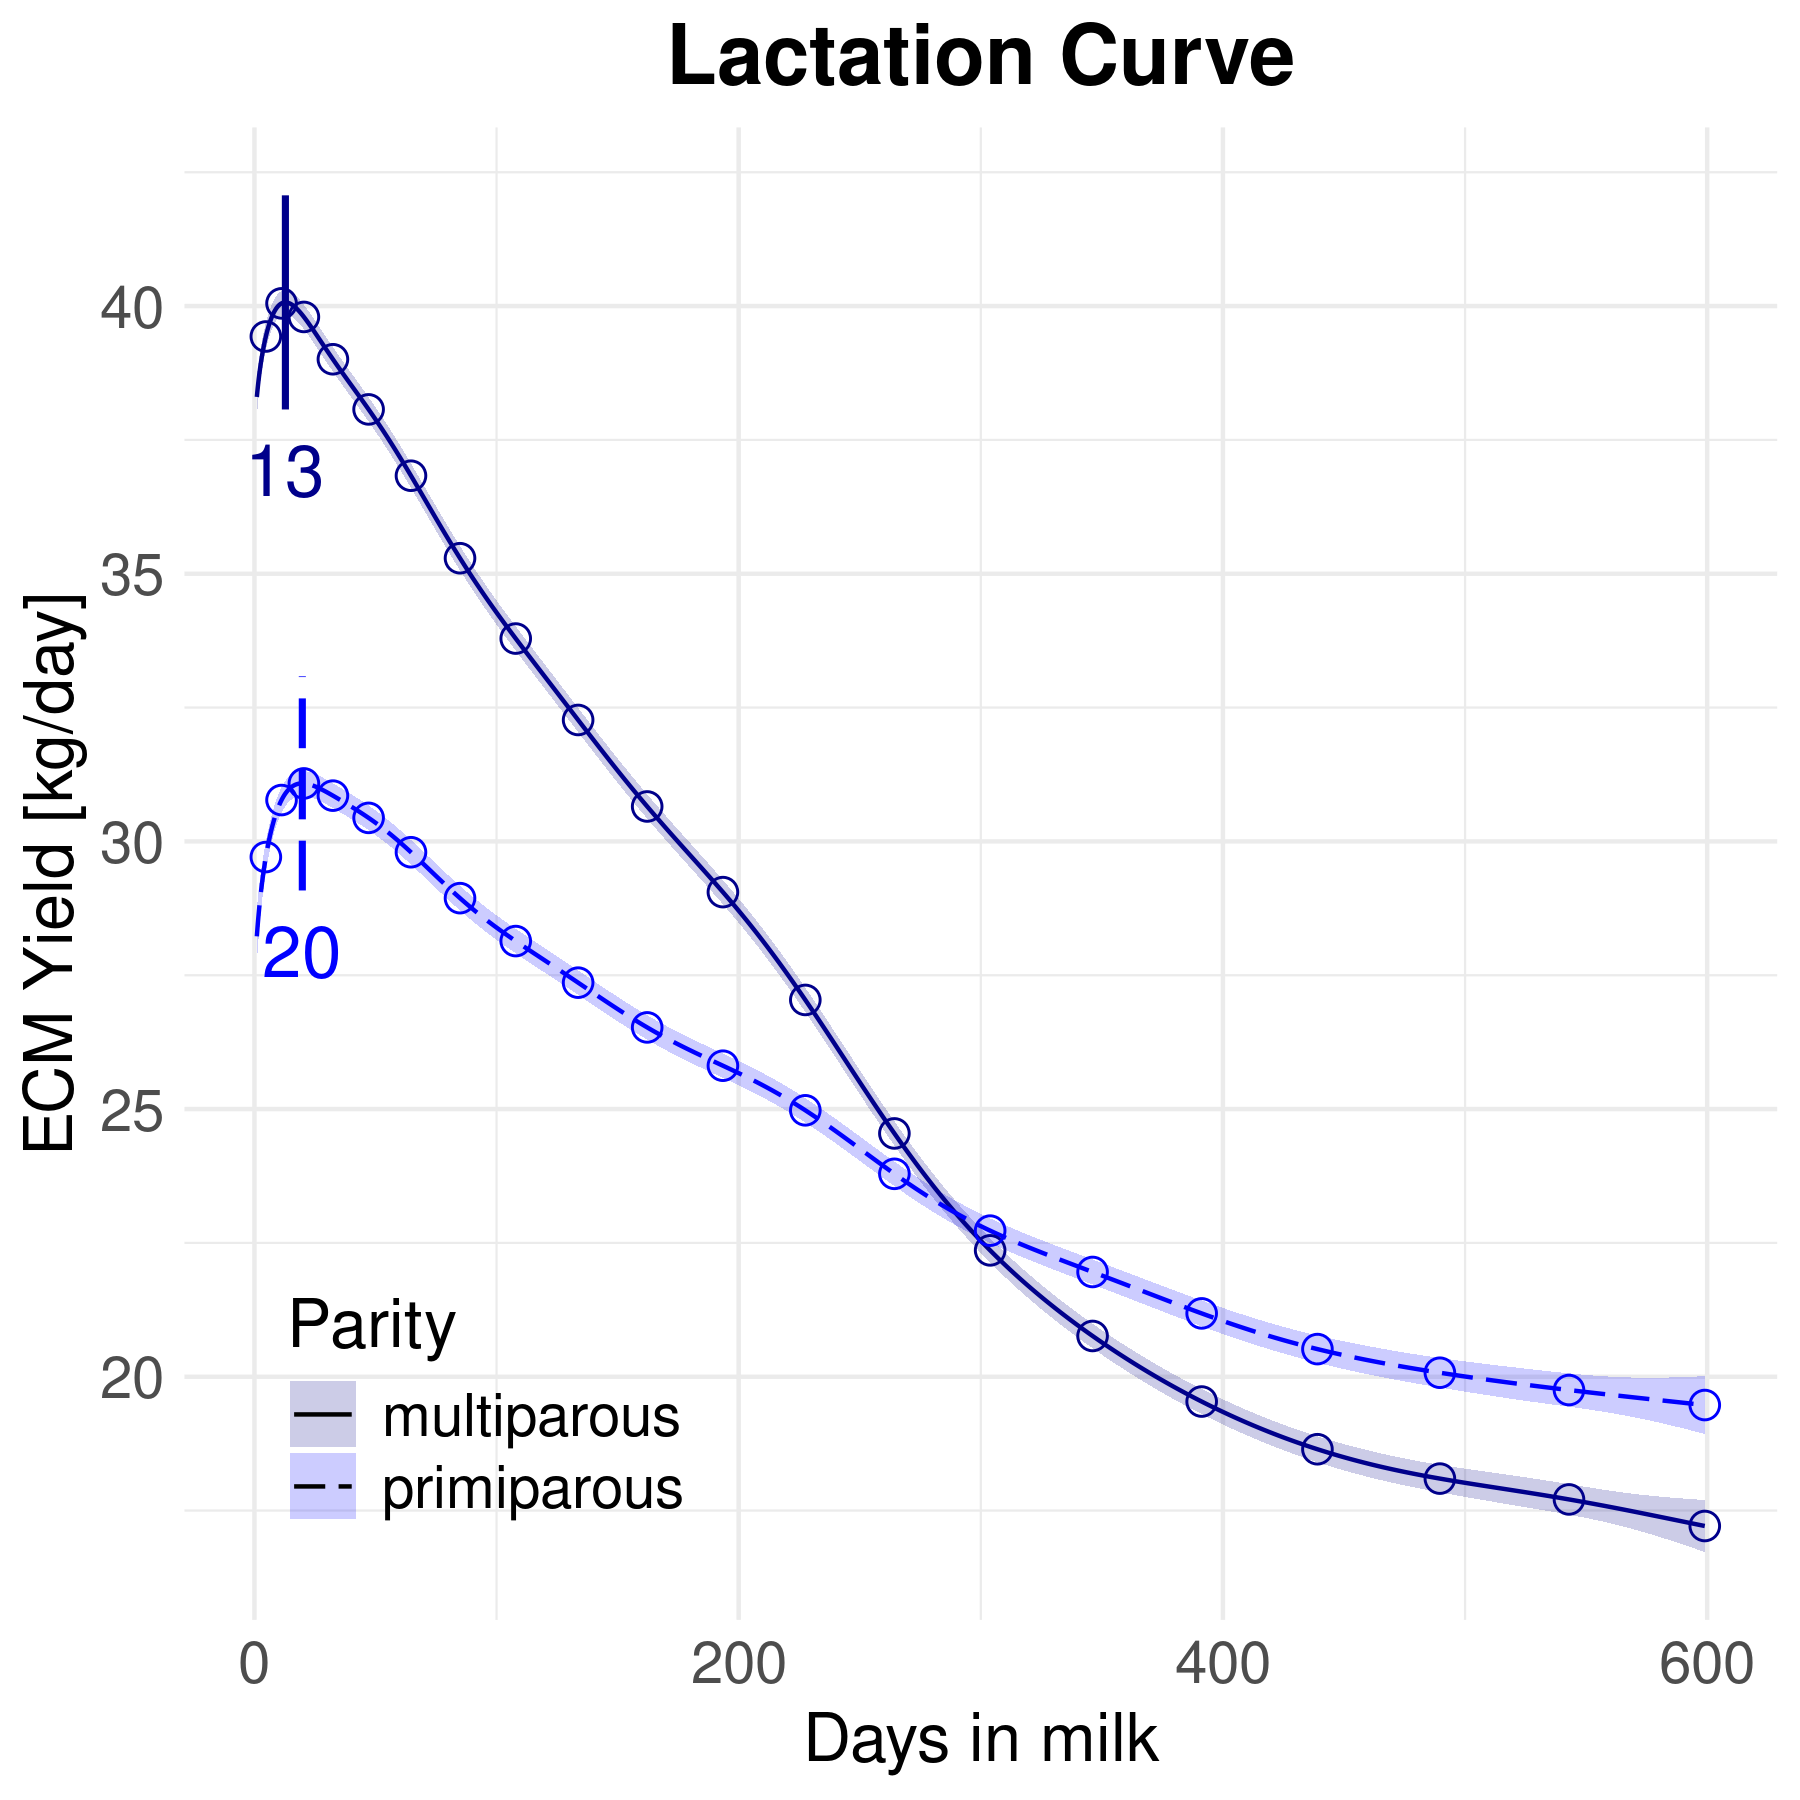
\includegraphics[width=\textwidth]{thesis/figures/models/ecm/full/ho_ecm_full/ho_ecm_full_marginal_dim_milk_combined.png}
    \end{subfigure}
    \begin{subfigure}[b]{0.45\textwidth}
        \centering
        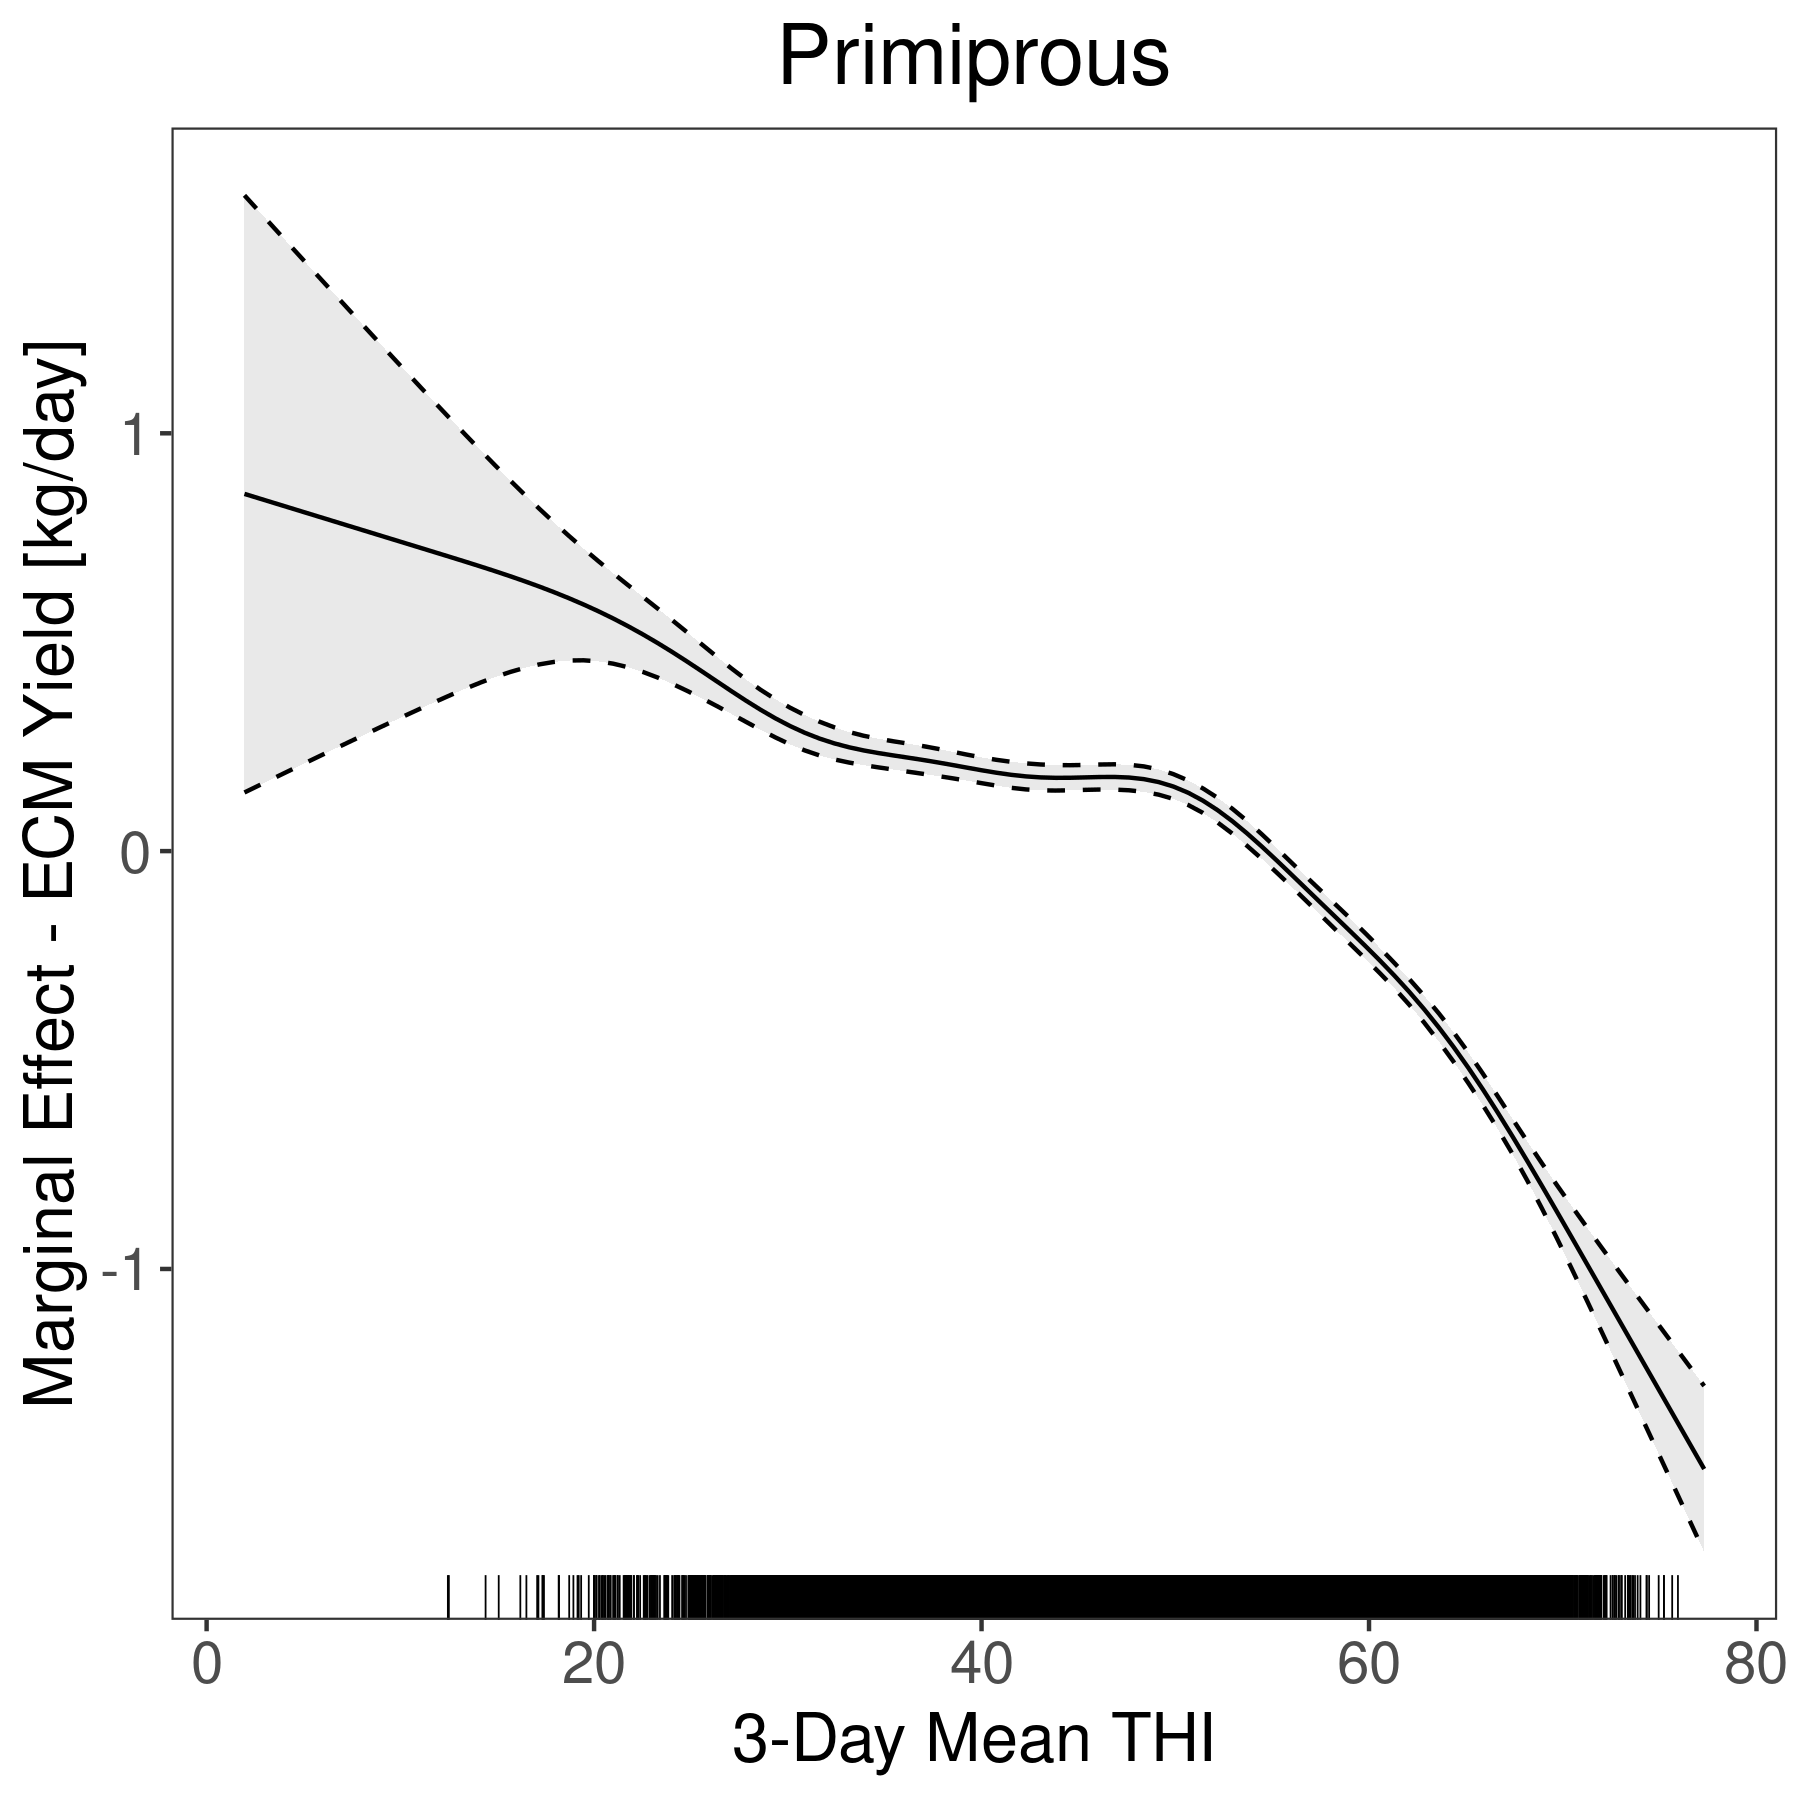
\includegraphics[width=\textwidth]{thesis/figures/models/ecm/full/ho_ecm_full/ho_ecm_full_marginal_thi_milk_primi.png}
    \end{subfigure}
    \hspace{0.05\textwidth} % Optional space between the figures
    \begin{subfigure}[b]{0.45\textwidth}
        \centering
        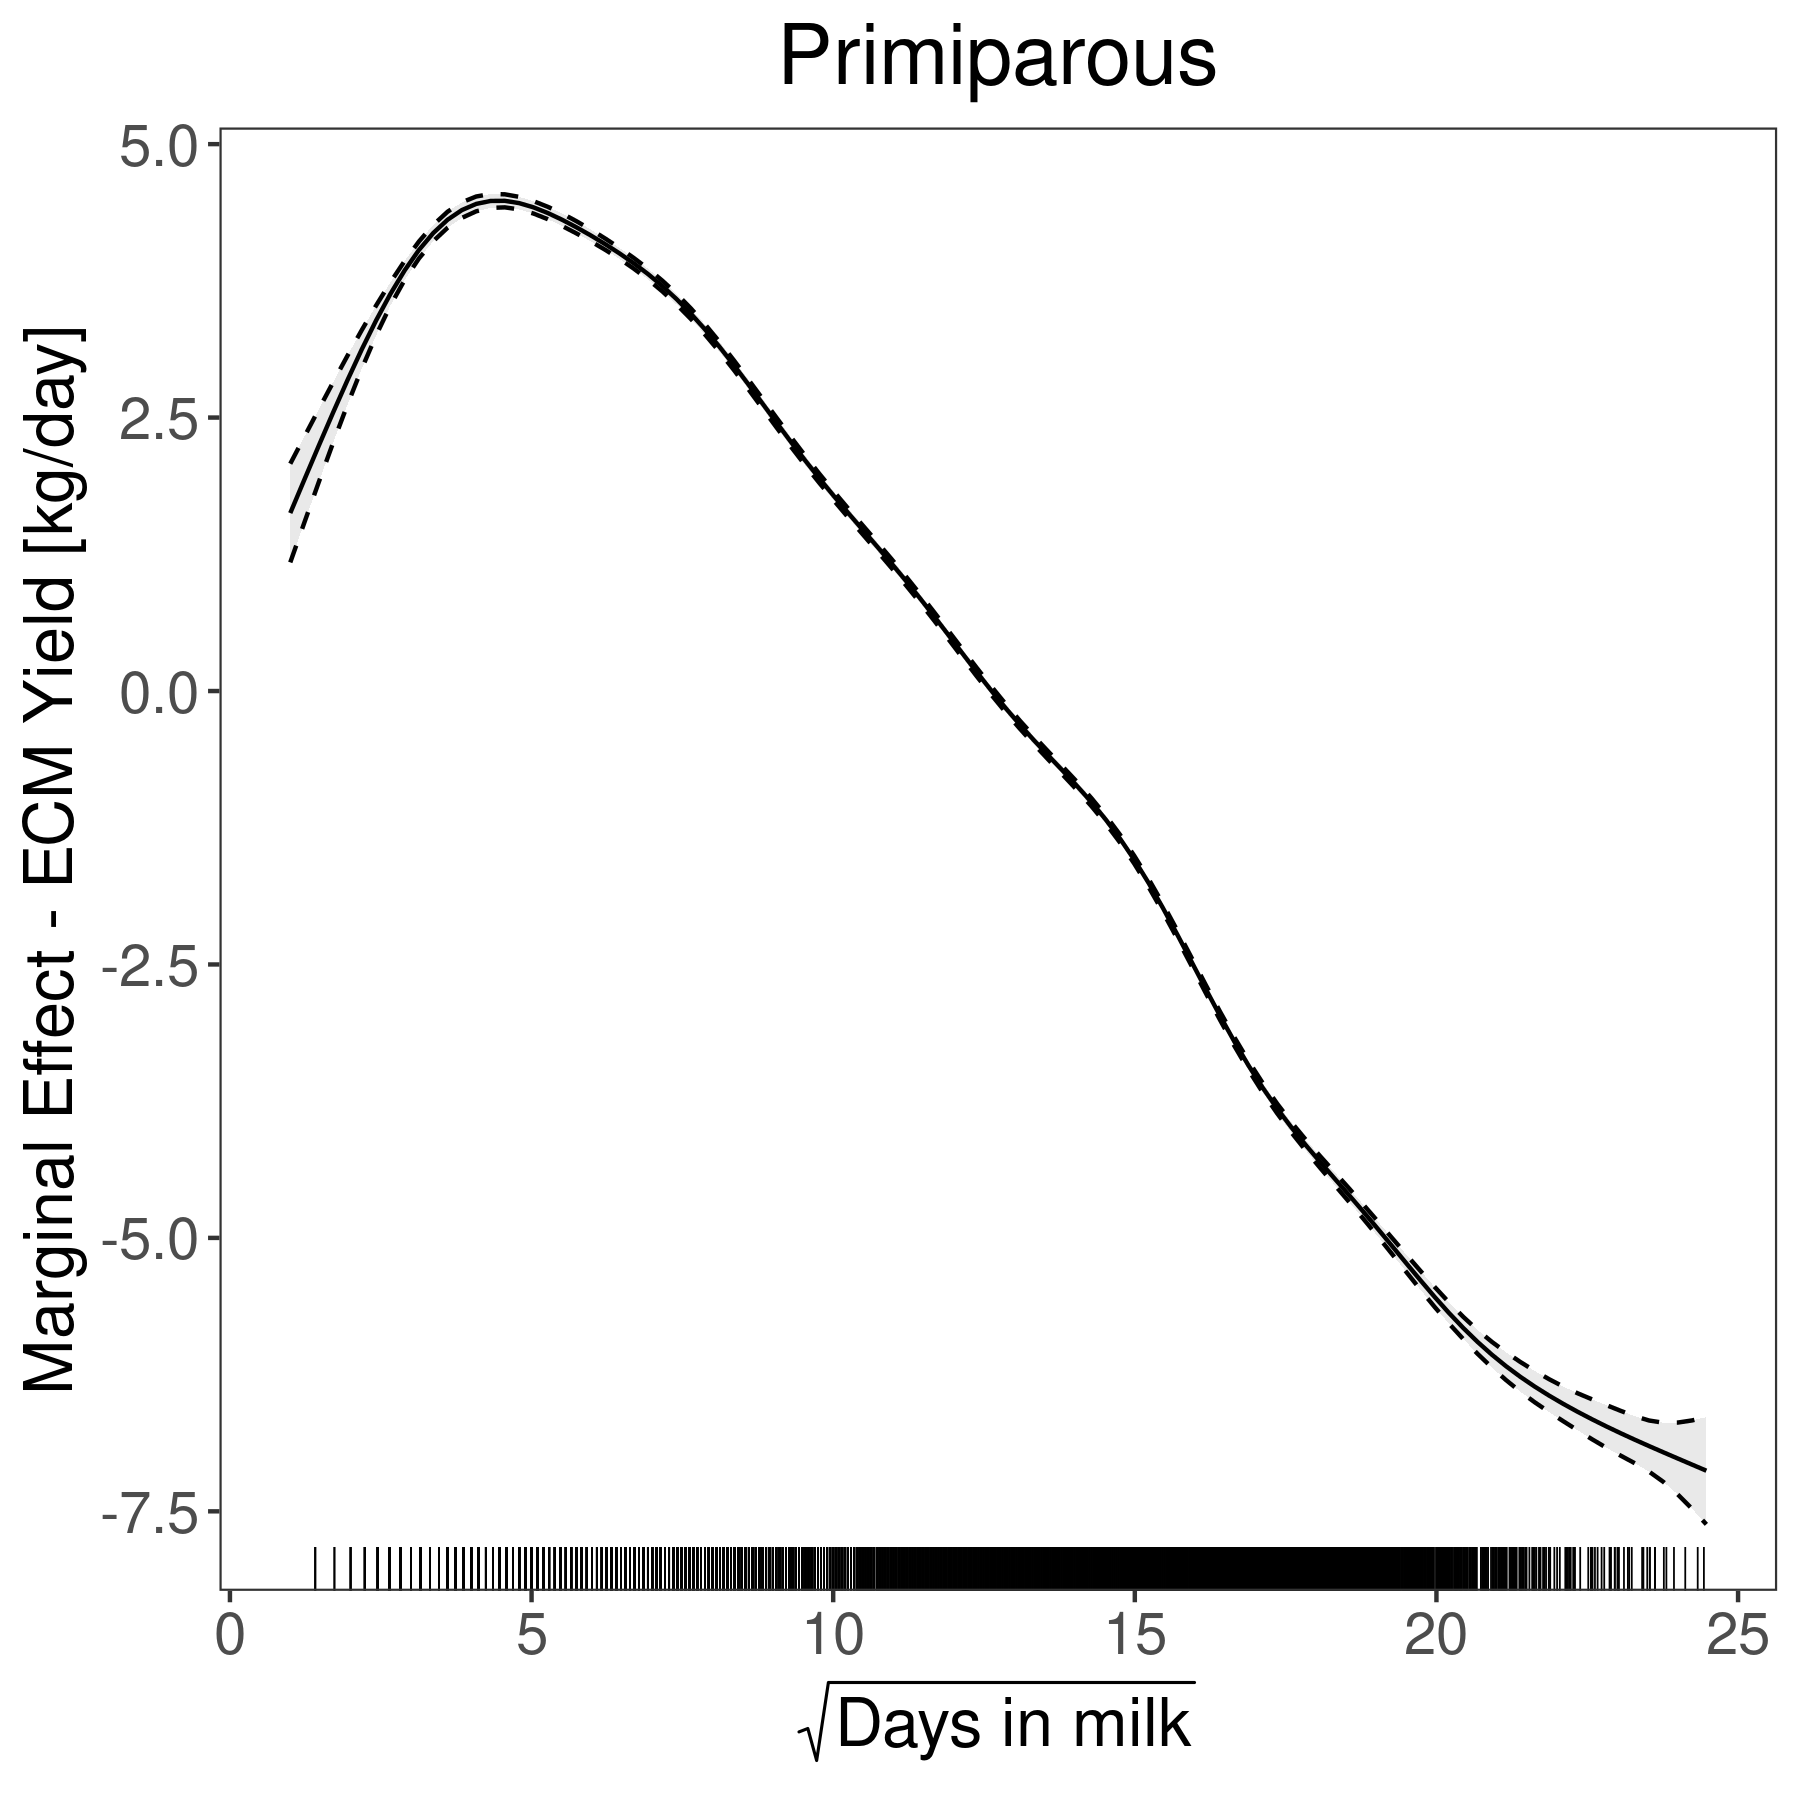
\includegraphics[width=\textwidth]{thesis/figures/models/ecm/full/ho_ecm_full/ho_ecm_full_marginal_dim_milk_primi.png}
    \end{subfigure}
    \begin{subfigure}[b]{0.45\textwidth}
        \centering
        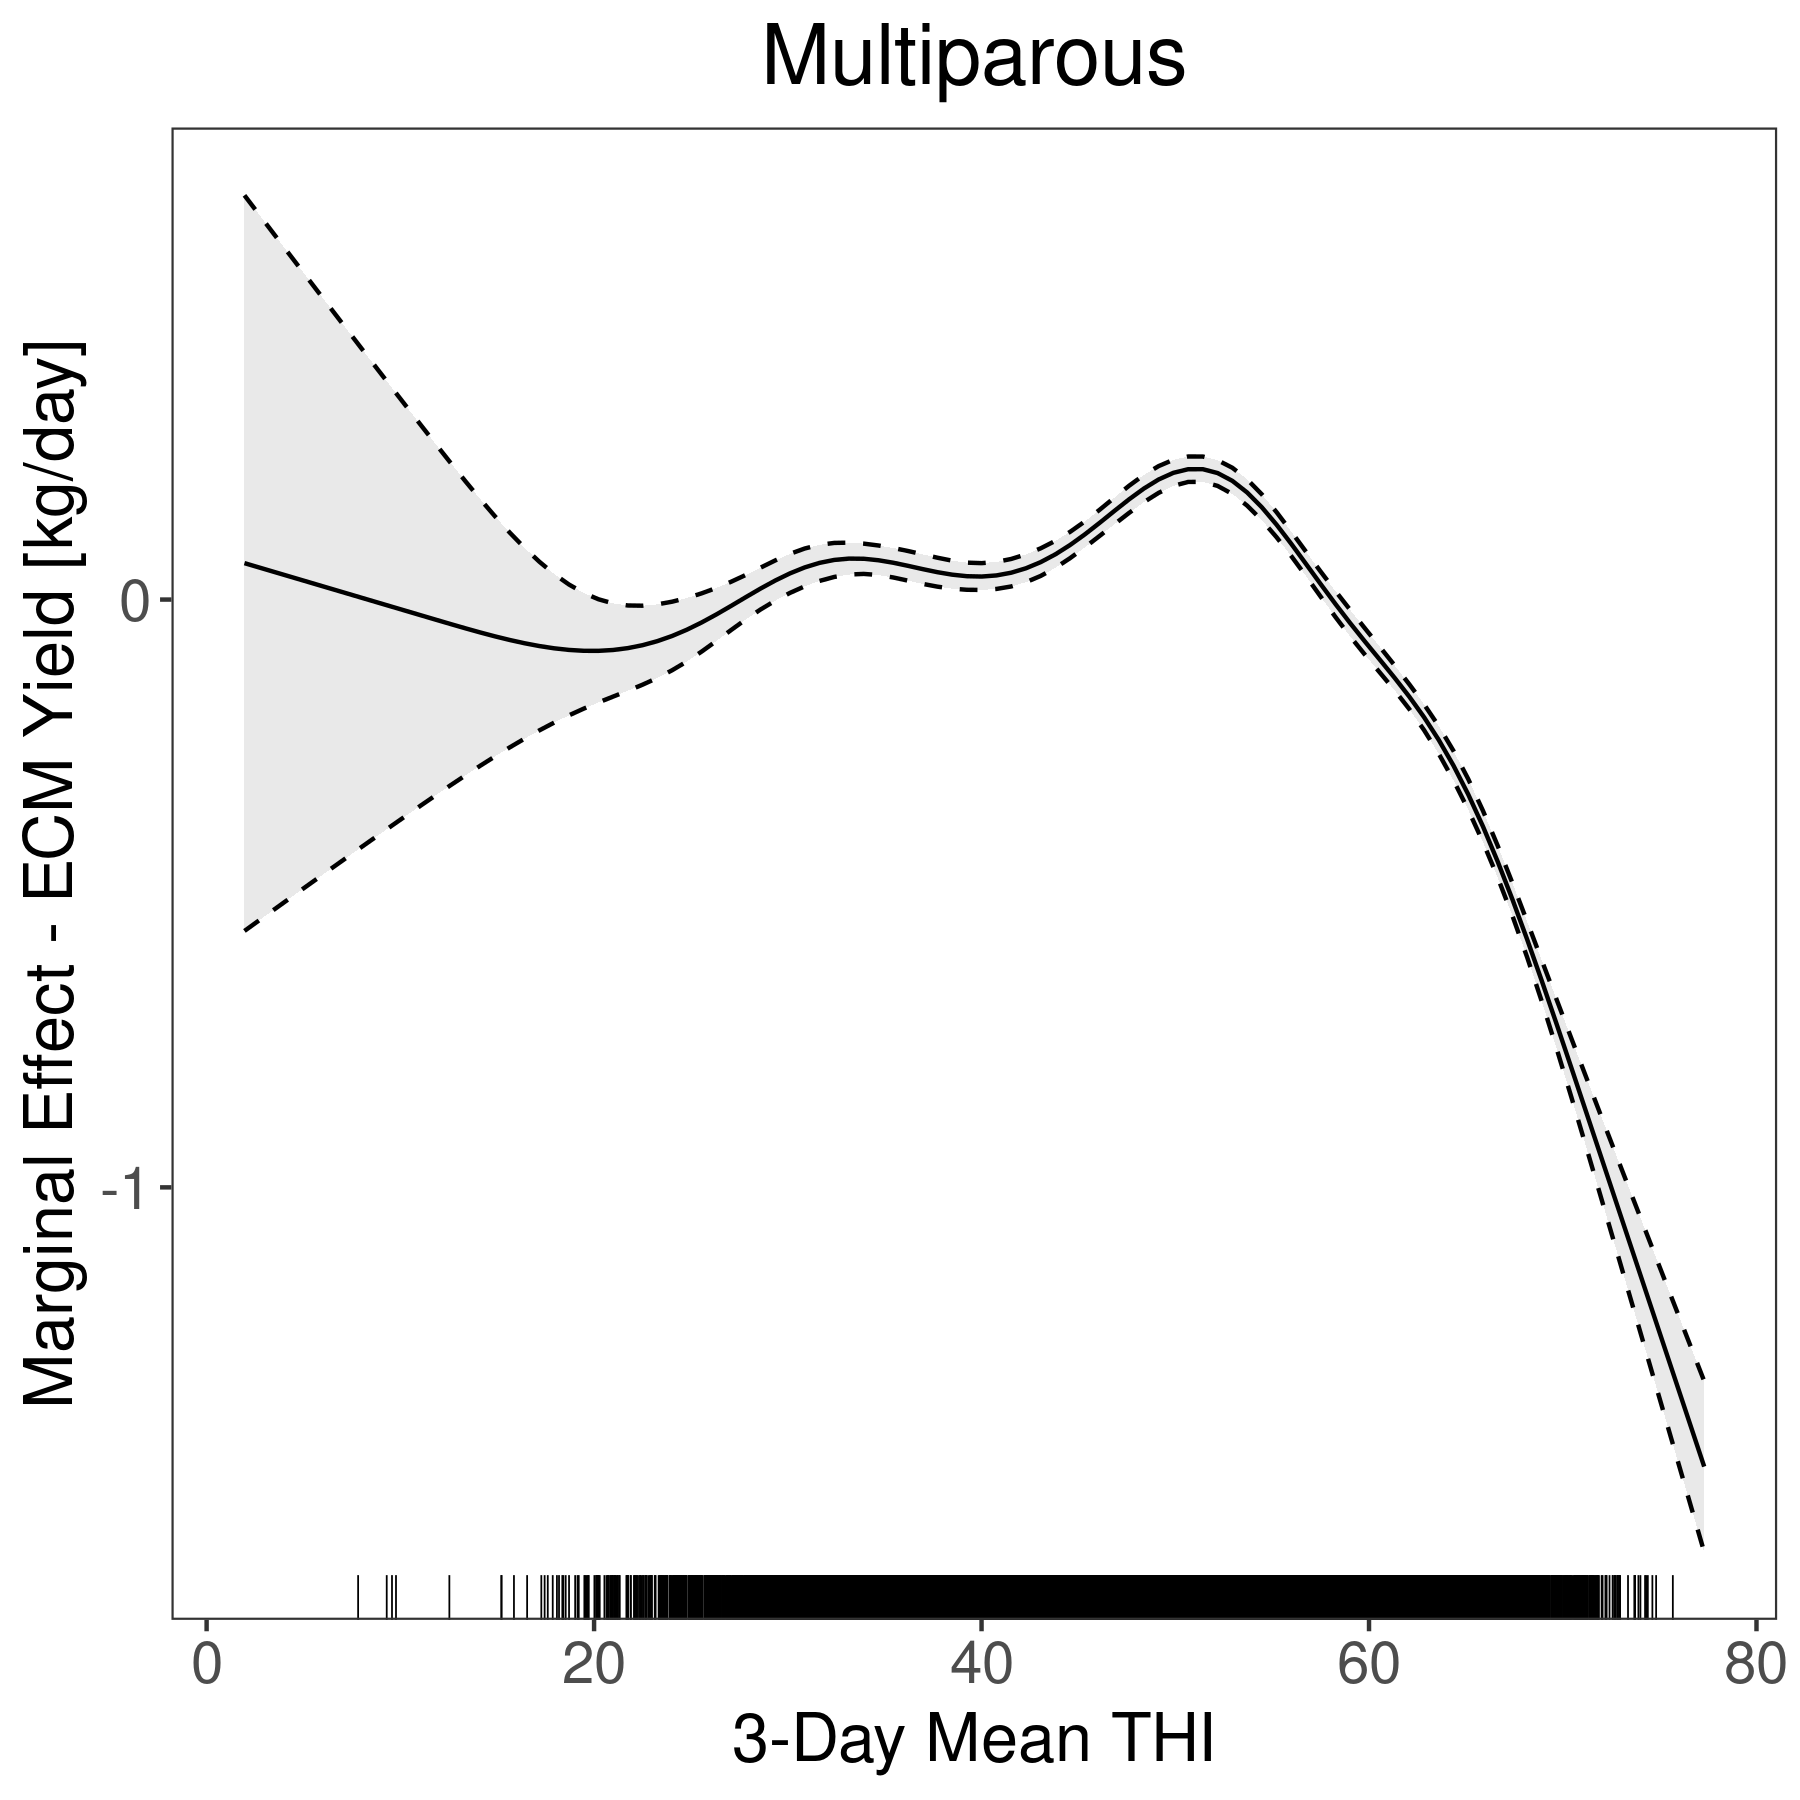
\includegraphics[width=\textwidth]{thesis/figures/models/ecm/full/ho_ecm_full/ho_ecm_full_marginal_thi_milk_multi.png}
    \end{subfigure}
    \hspace{0.05\textwidth} % Optional space between the figures
    \begin{subfigure}[b]{0.45\textwidth}
        \centering
        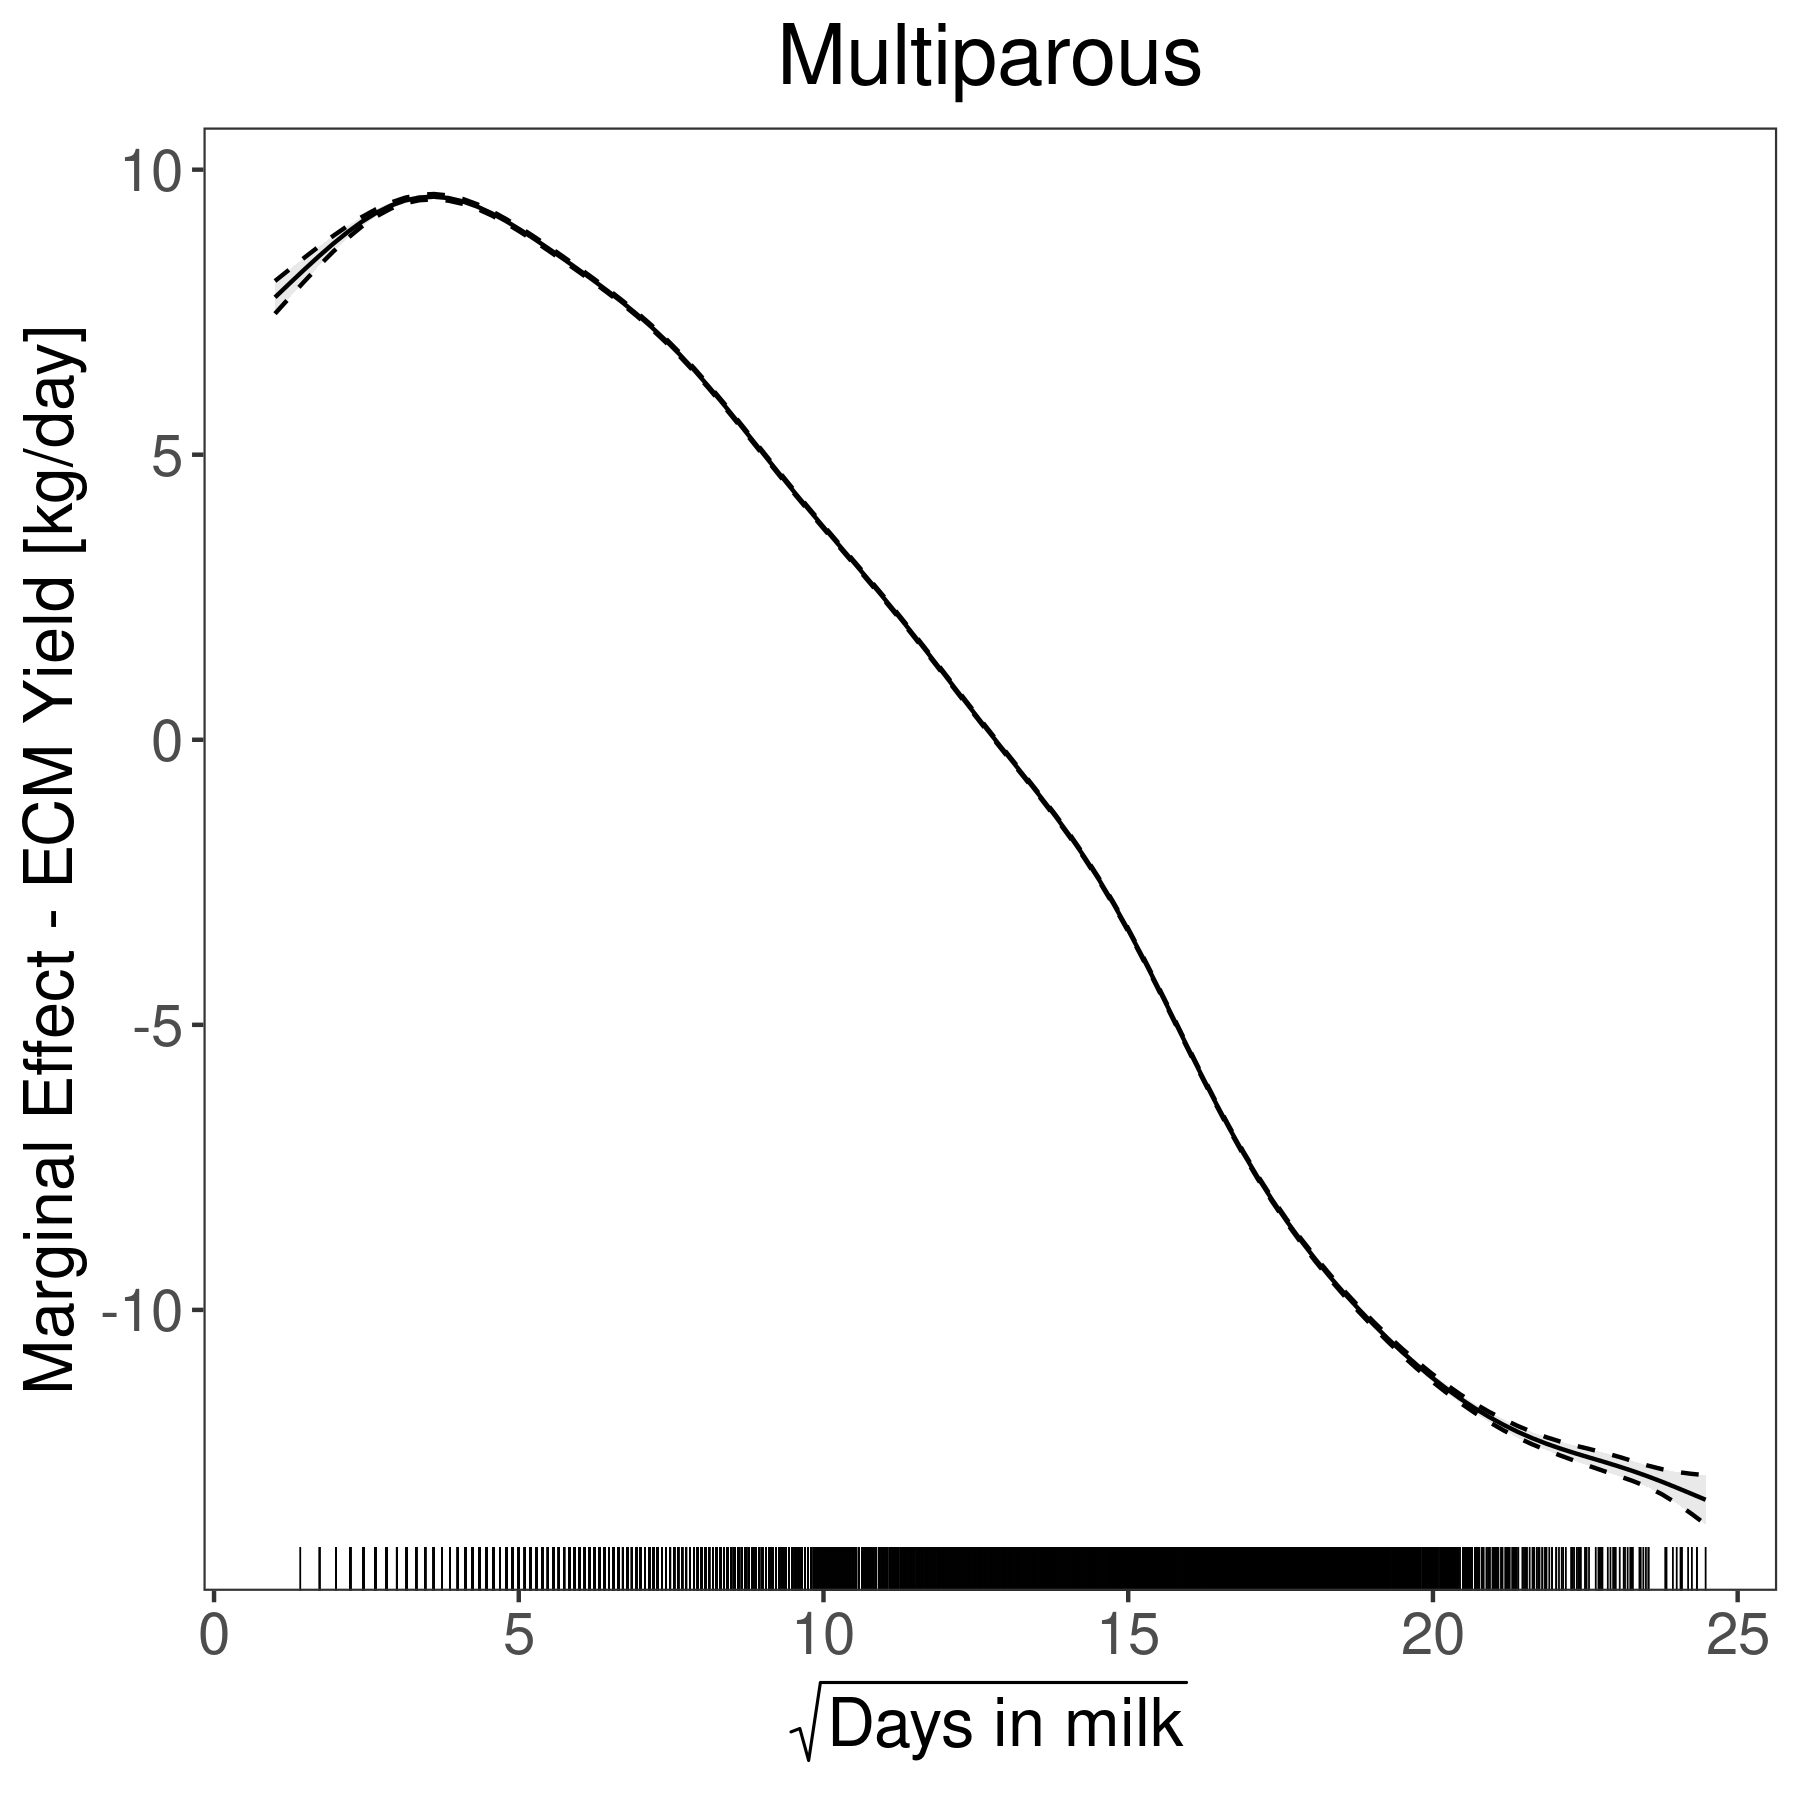
\includegraphics[width=\textwidth]{thesis/figures/models/ecm/full/ho_ecm_full/ho_ecm_full_marginal_dim_milk_multi.png}
    \end{subfigure}
    \caption[]{Holstein: ECM Yield - 1985 - 2023 - THI Effect and Lactation Curve}
    \label{fig:main}
\end{figure}


\subsection{Split Period: Until 2010 - After 2010}
\addtocontents{toc}{\protect\setcounter{tocdepth}{-1}}
\subsubsection{Split Period: 1985 - 2010}\label{model:ho_ecm_before}

\paragraph{Model Summary} \quad \\

    \begin{table}[H]
    \centering
    \begin{tabular}{lrrrr}
    \textbf{A. parametric coefficients} & Estimate & Std. Error & t-value & p-value \\ 
       \hline
       \hline
  (Intercept) & 19.5611 & 0.4528 & 43.2033 & $<$ 0.0001 \\ 
  parityprimiparous & -3.4047 & 0.0125 & -272.5784 & $<$ 0.0001 \\ 
  year1986 & 0.1564 & 0.2983 & 0.5244 & 0.6000 \\ 
  year1987 & -0.1604 & 0.3786 & -0.4236 & 0.6718 \\ 
  year1988 & -0.4125 & 0.4604 & -0.8959 & 0.3703 \\ 
  year1989 & 0.2840 & 0.4787 & 0.5933 & 0.5530 \\ 
  year1990 & 0.8561 & 0.5110 & 1.6753 & 0.0939 \\ 
  year1991 & 1.2054 & 0.5295 & 2.2764 & 0.0228 \\ 
  year1992 & 1.5896 & 0.4714 & 3.3720 & 0.0007 \\ 
  year1993 & 1.7199 & 0.4841 & 3.5526 & 0.0004 \\ 
  year1994 & 1.5862 & 0.4844 & 3.2746 & 0.0011 \\ 
  year1995 & 1.9400 & 0.4862 & 3.9899 & 0.0001 \\ 
  year1996 & 2.3149 & 0.4891 & 4.7332 & $<$ 0.0001 \\ 
  year1997 & 2.8495 & 0.4910 & 5.8030 & $<$ 0.0001 \\ 
  year1998 & 3.4994 & 0.4911 & 7.1260 & $<$ 0.0001 \\ 
  year1999 & 3.4311 & 0.4857 & 7.0648 & $<$ 0.0001 \\ 
  year2000 & 3.4183 & 0.4792 & 7.1327 & $<$ 0.0001 \\ 
  year2001 & 3.8865 & 0.4810 & 8.0803 & $<$ 0.0001 \\ 
  year2002 & 3.9895 & 0.4914 & 8.1191 & $<$ 0.0001 \\ 
  year2003 & 4.4780 & 0.4786 & 9.3555 & $<$ 0.0001 \\ 
  year2004 & 5.1219 & 0.4755 & 10.7715 & $<$ 0.0001 \\ 
  year2005 & 5.7371 & 0.4721 & 12.1526 & $<$ 0.0001 \\ 
  year2006 & 5.8086 & 0.4726 & 12.2895 & $<$ 0.0001 \\ 
  year2007 & 5.7180 & 0.4751 & 12.0362 & $<$ 0.0001 \\ 
  year2008 & 6.2530 & 0.4793 & 13.0457 & $<$ 0.0001 \\ 
  year2009 & 6.9507 & 0.4640 & 14.9808 & $<$ 0.0001 \\ 
  year2010 & 7.7630 & 0.4885 & 15.8912 & $<$ 0.0001 \\
       \hline
    \textbf{B. smooth terms} & edf & Ref.df & F-value & p-value \\ 
    \hline
    \hline
  s(thi\_mean\_t0\_3d):paritymultiparous & 8.4826 & 8.4826 & 267.5958 & $<$ 0.0001 \\ 
  s(thi\_mean\_t0\_3d):parityprimiparous & 7.6228 & 7.6228 & 298.9671 & $<$ 0.0001 \\ 
  s(days\_in\_milk\_t):paritymultiparous & 13.4714 & 13.4714 & 151697.0514 & $<$ 0.0001 \\ 
  s(days\_in\_milk\_t):parityprimiparous & 12.5410 & 12.5410 & 17254.6016 & $<$ 0.0001 \\
       \hline
    \end{tabular}
    \caption[]{Holstein: ECM Yield - 1985-2010 - GAMM model summary without random effect terms.}
    \end{table}

\newpage
\begin{table}[H]
\centering
\begin{tabular}
{l | r | r | r | r}
\textbf{Smooth Term Fixed Effect} & Est. & SE & z & p\\
\hline
\hline
s(thi\_mean\_t0\_3d):multiFx1 & 0.4794 & 0.1132 & 4.23 & $<$ 1e-04 \\
s(thi\_mean\_t0\_3d):primiFx1 & 0.4898 & 0.1339 & 3.66 & 0.0003\\
s(days\_in\_milk\_):multiFx1 &  -1.1736 & 0.4499 & -2.61 & 0.0091\\
s(days\_in\_milk\_):primiFx1 & 0.3524 & 0.4318 & 0.82 & 0.4144\\
\hline
\textbf{Variance Component} & Estimated $\sigma$ & & & \\
\hline
\hline
$\sigma_\alpha$ & 2.9719 & &  & \\
$\sigma_\iota$ & 1.0261 & & & \\
$\sigma_\phi$ & 3.0716 & & & \\
s(thi\_mean\_t0\_3d):multi & 2.4372 & & & \\
s(days\_in\_milk\_):primi & 4.3089 & & & \\
s(days\_in\_milk\_):multi & 7.2579 & & & \\
s(thi\_mean\_t0\_3d):primi & 1.8041 & & & \\
Residual & 3.7828 & & & \\
\end{tabular}
\caption[]{Holstein: ECM Yield - 1985-2010 - Mixed Model Summary - Smooth Terms and Random Effects.}
\end{table}

\paragraph{Model Diagnostics} \quad \\
\begin{figure}[H]
    \centering
    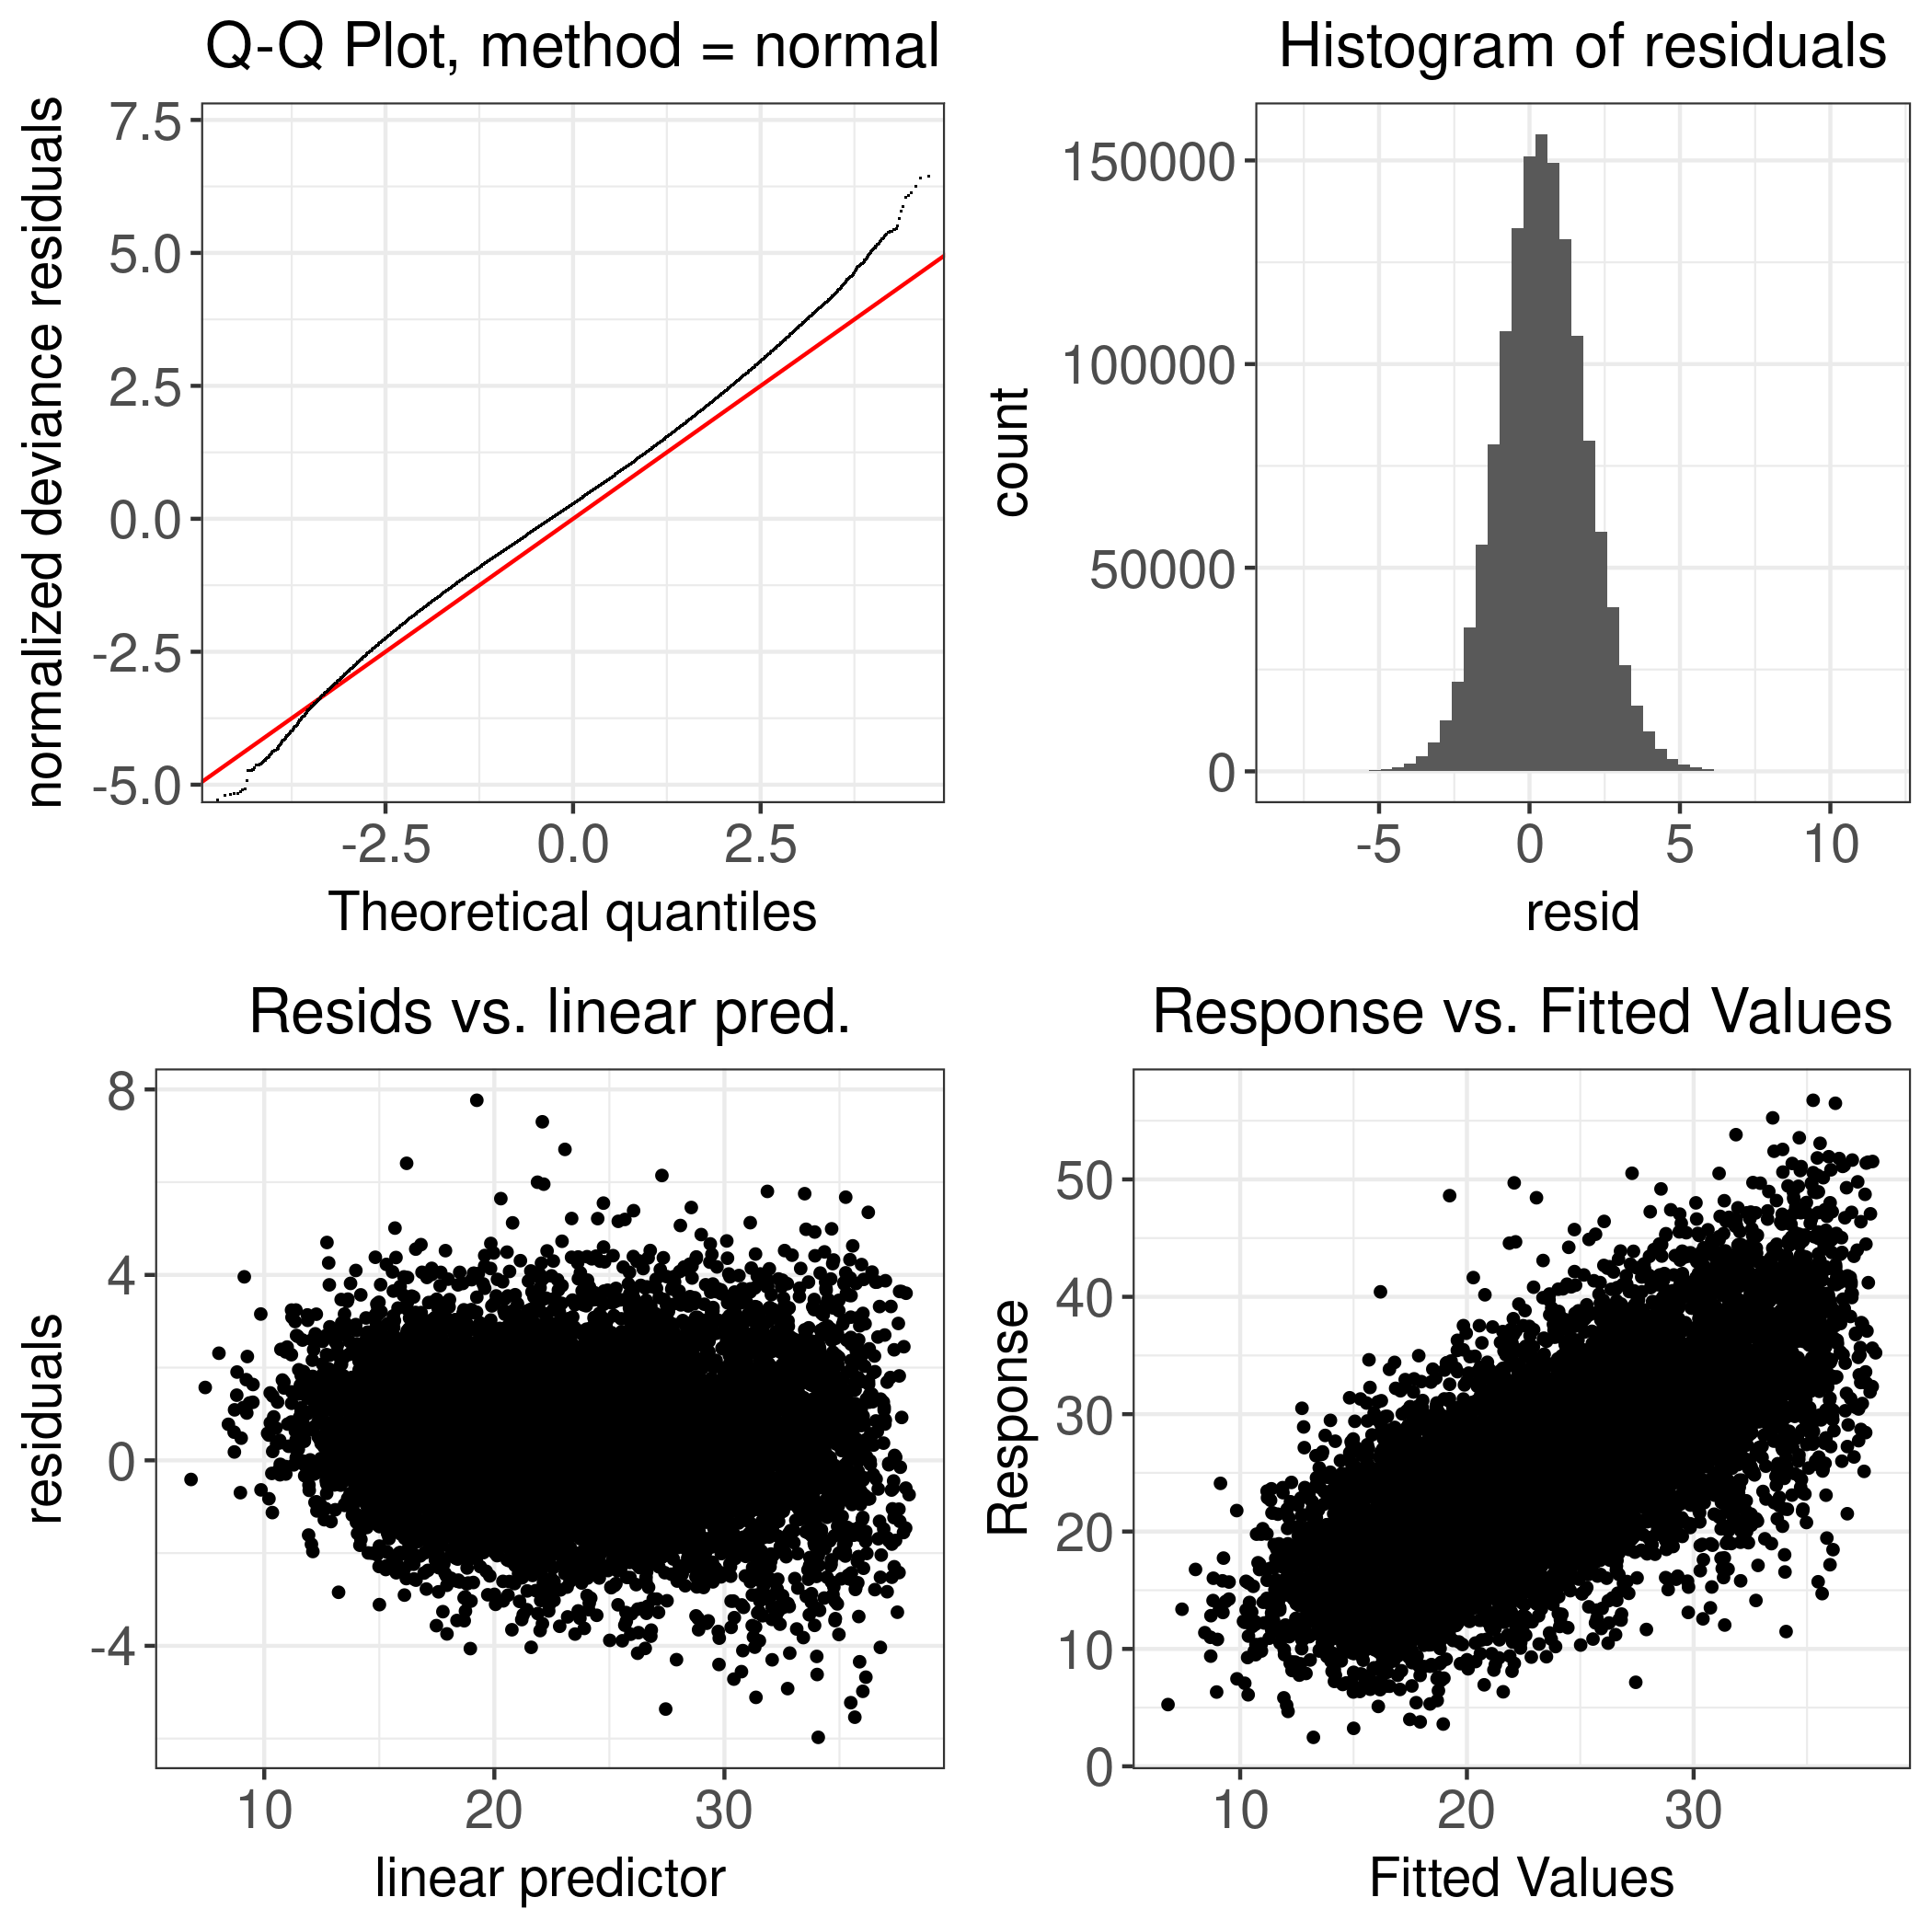
\includegraphics[width=0.6\textwidth]{thesis/figures/models/ecm/before2010/ho_ecm_before2010/ho_ecm_before2010_diagnostics.png}
    \caption[]{Holstein: ECM Yield - 1985-2010 - Diagnostic Plot}
\end{figure}

\newpage
\paragraph{THI Effect and Lactation Curve} \quad \\
\begin{figure}[H]
    \centering
    \begin{subfigure}[b]{0.45\textwidth}
        \centering
        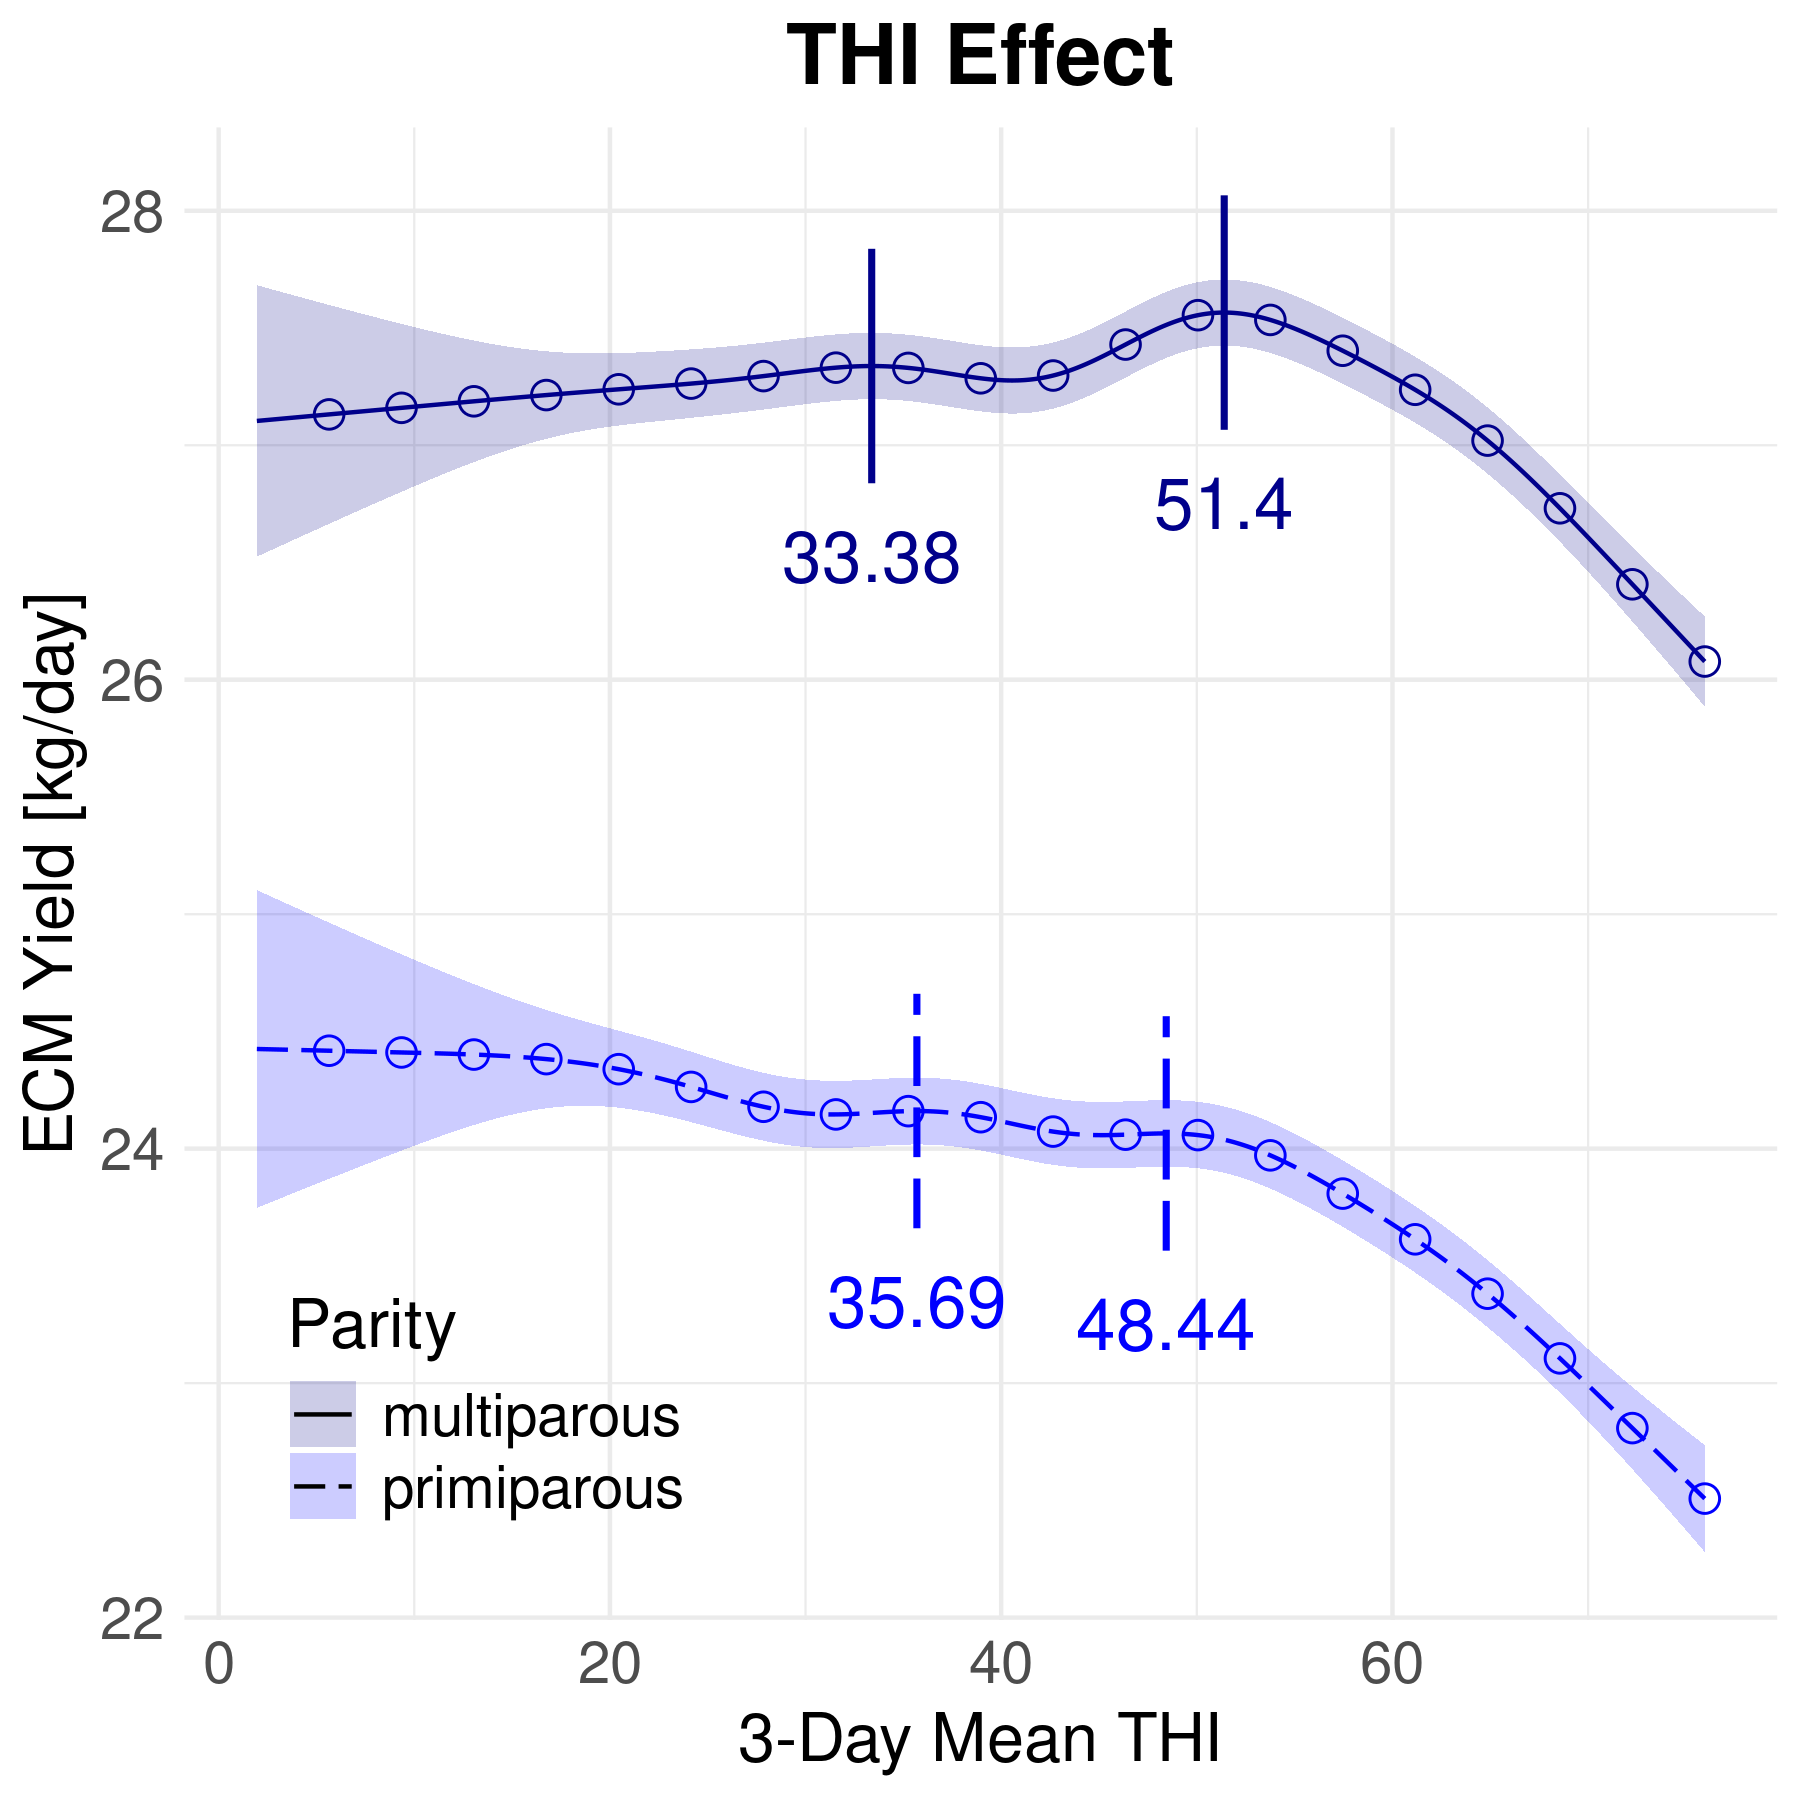
\includegraphics[width=\textwidth]{thesis/figures/models/ecm/before2010/ho_ecm_before2010/ho_ecm_before2010_marginal_thi_milk_combined.png}
    \end{subfigure}
    \hspace{0.05\textwidth} % Optional space between the figures
    \begin{subfigure}[b]{0.45\textwidth}
        \centering
        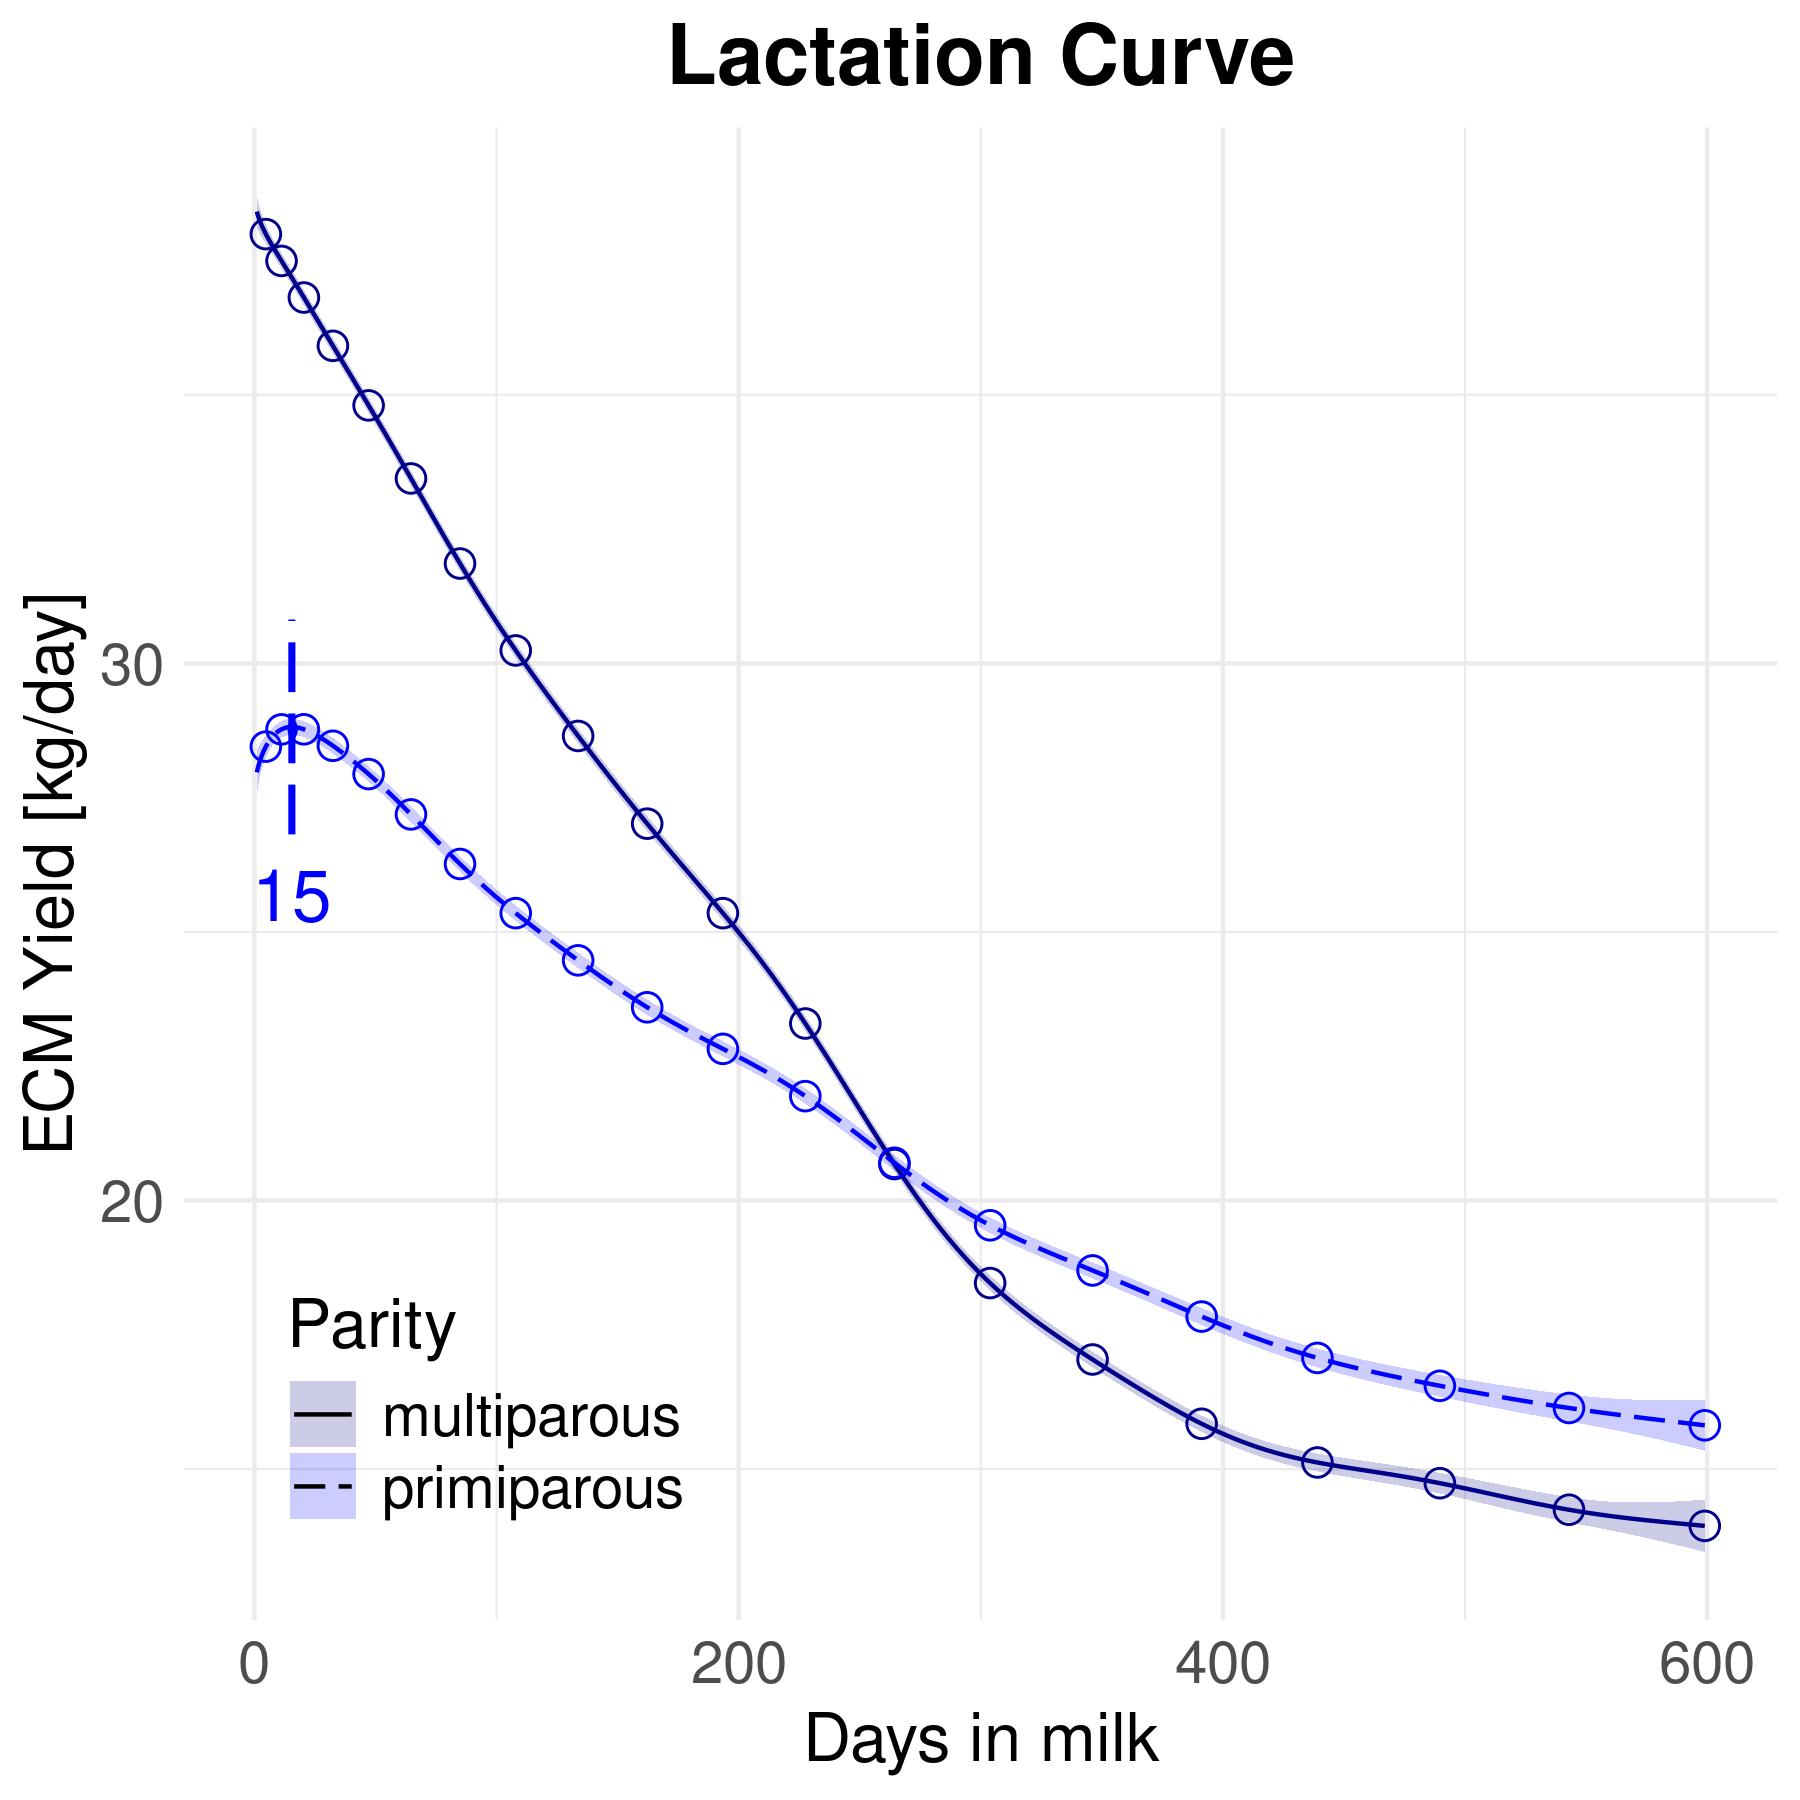
\includegraphics[width=\textwidth]{thesis/figures/models/ecm/before2010/ho_ecm_before2010/ho_ecm_before2010_marginal_dim_milk_combined.png}
    \end{subfigure}
    \begin{subfigure}[b]{0.45\textwidth}
        \centering
        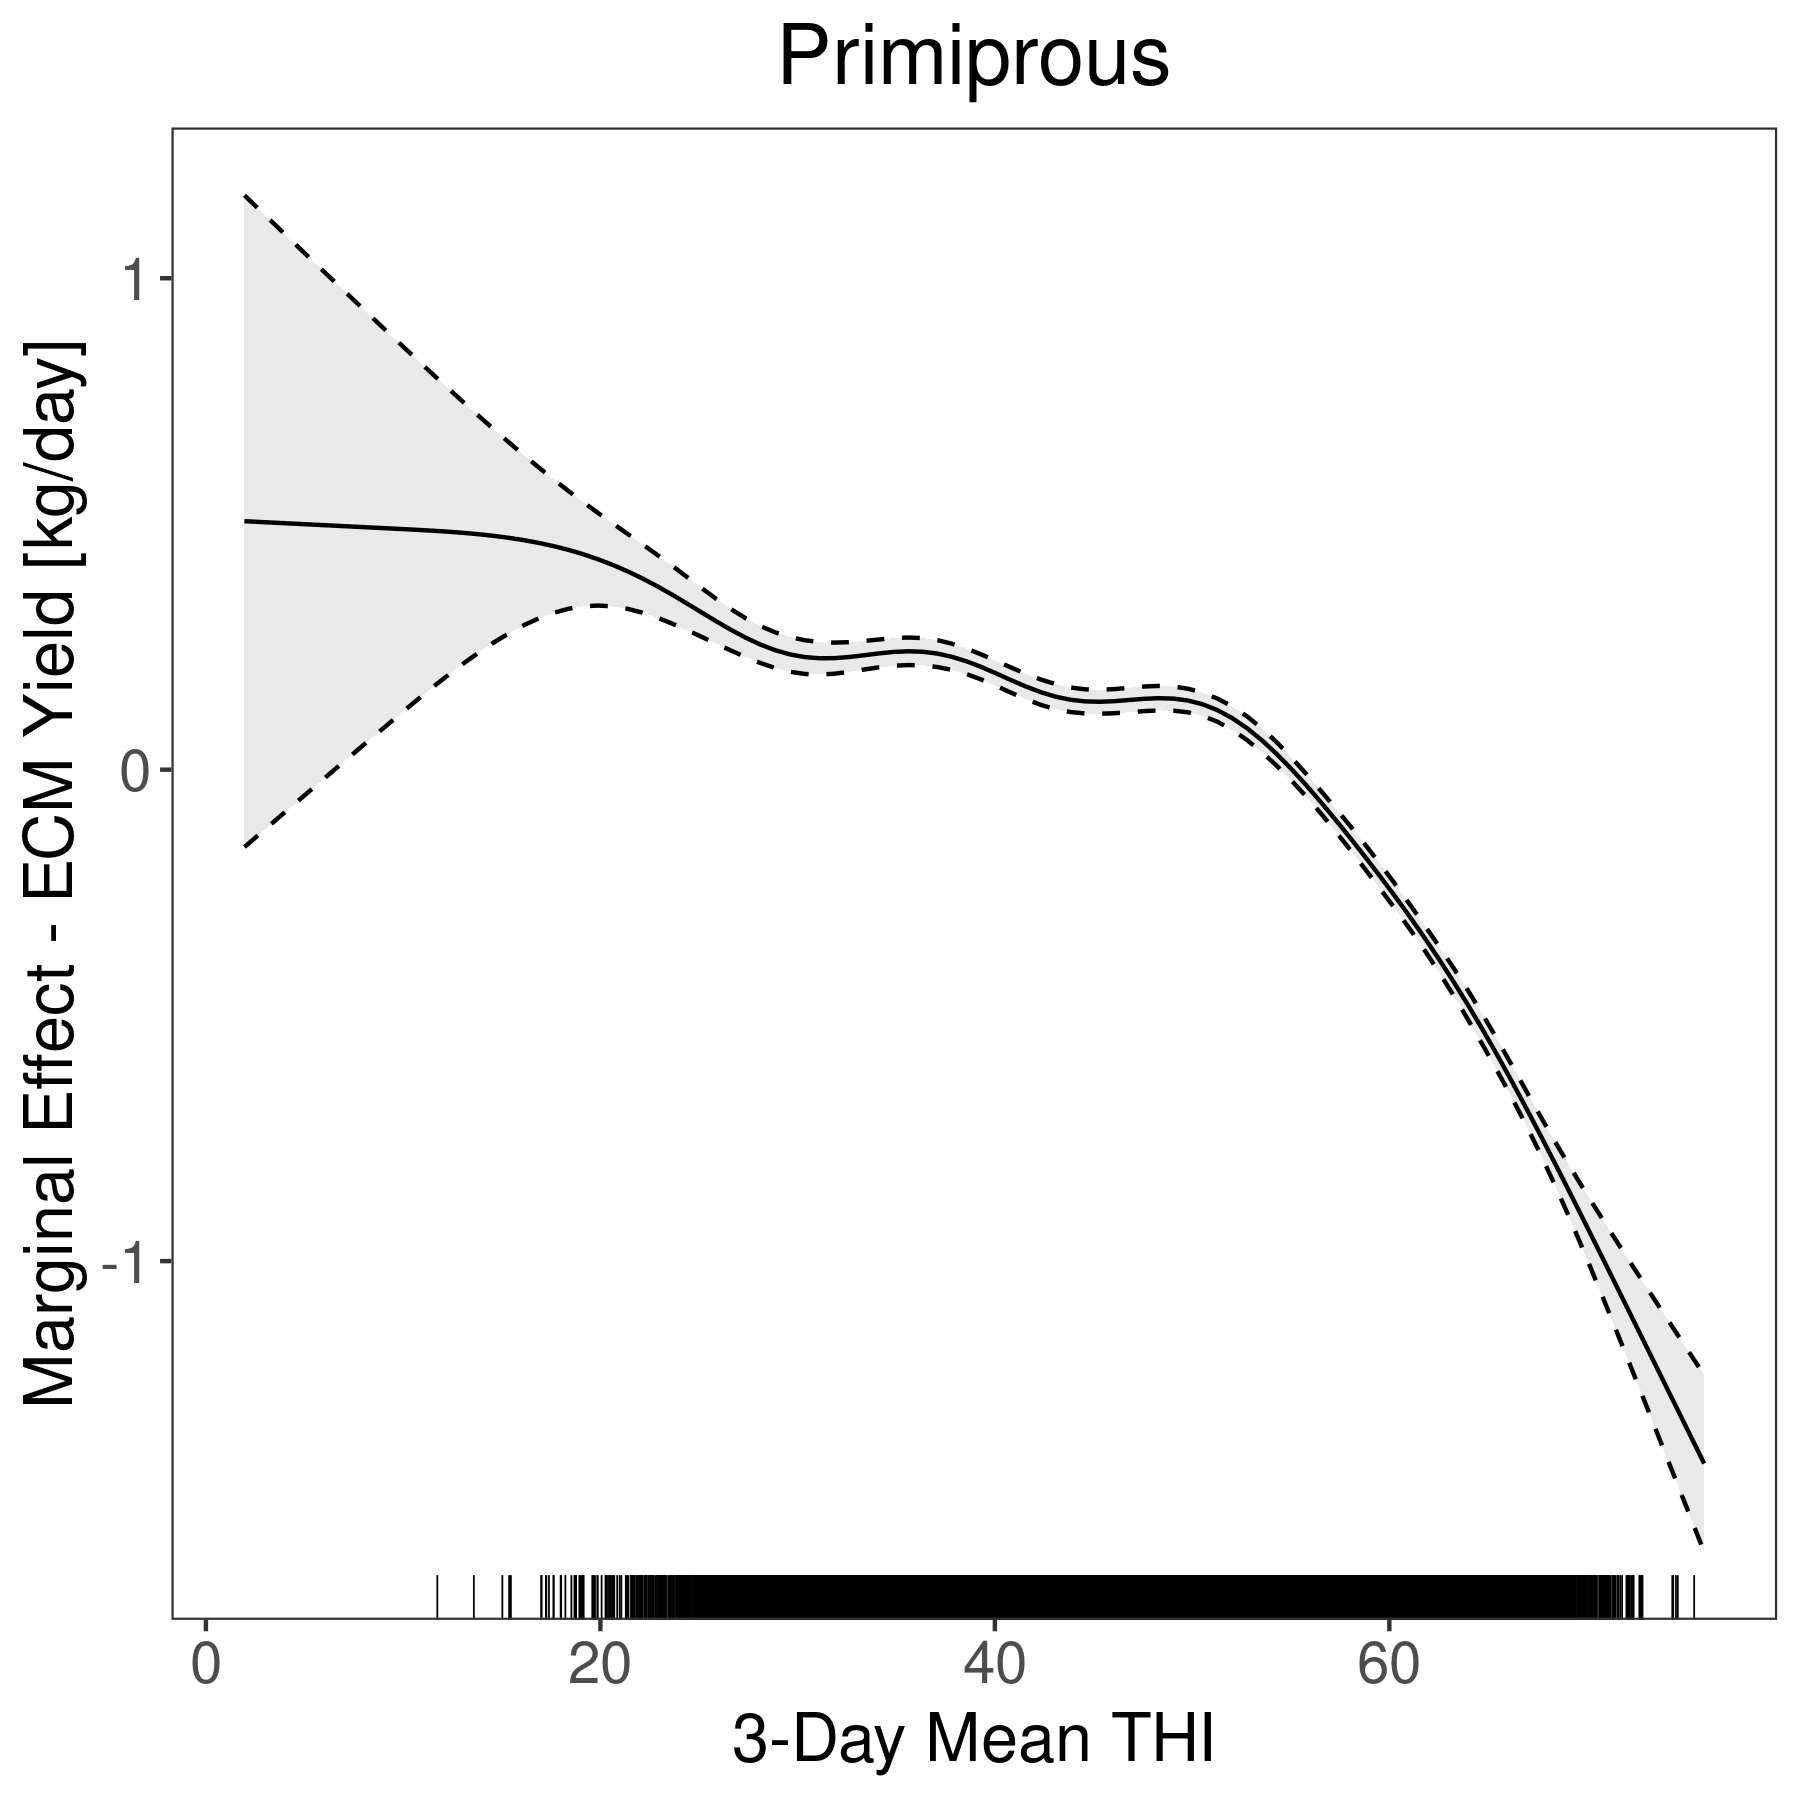
\includegraphics[width=\textwidth]{thesis/figures/models/ecm/before2010/ho_ecm_before2010/ho_ecm_before2010_marginal_thi_milk_primi.png}
    \end{subfigure}
    \hspace{0.05\textwidth} % Optional space between the figures
    \begin{subfigure}[b]{0.45\textwidth}
        \centering
        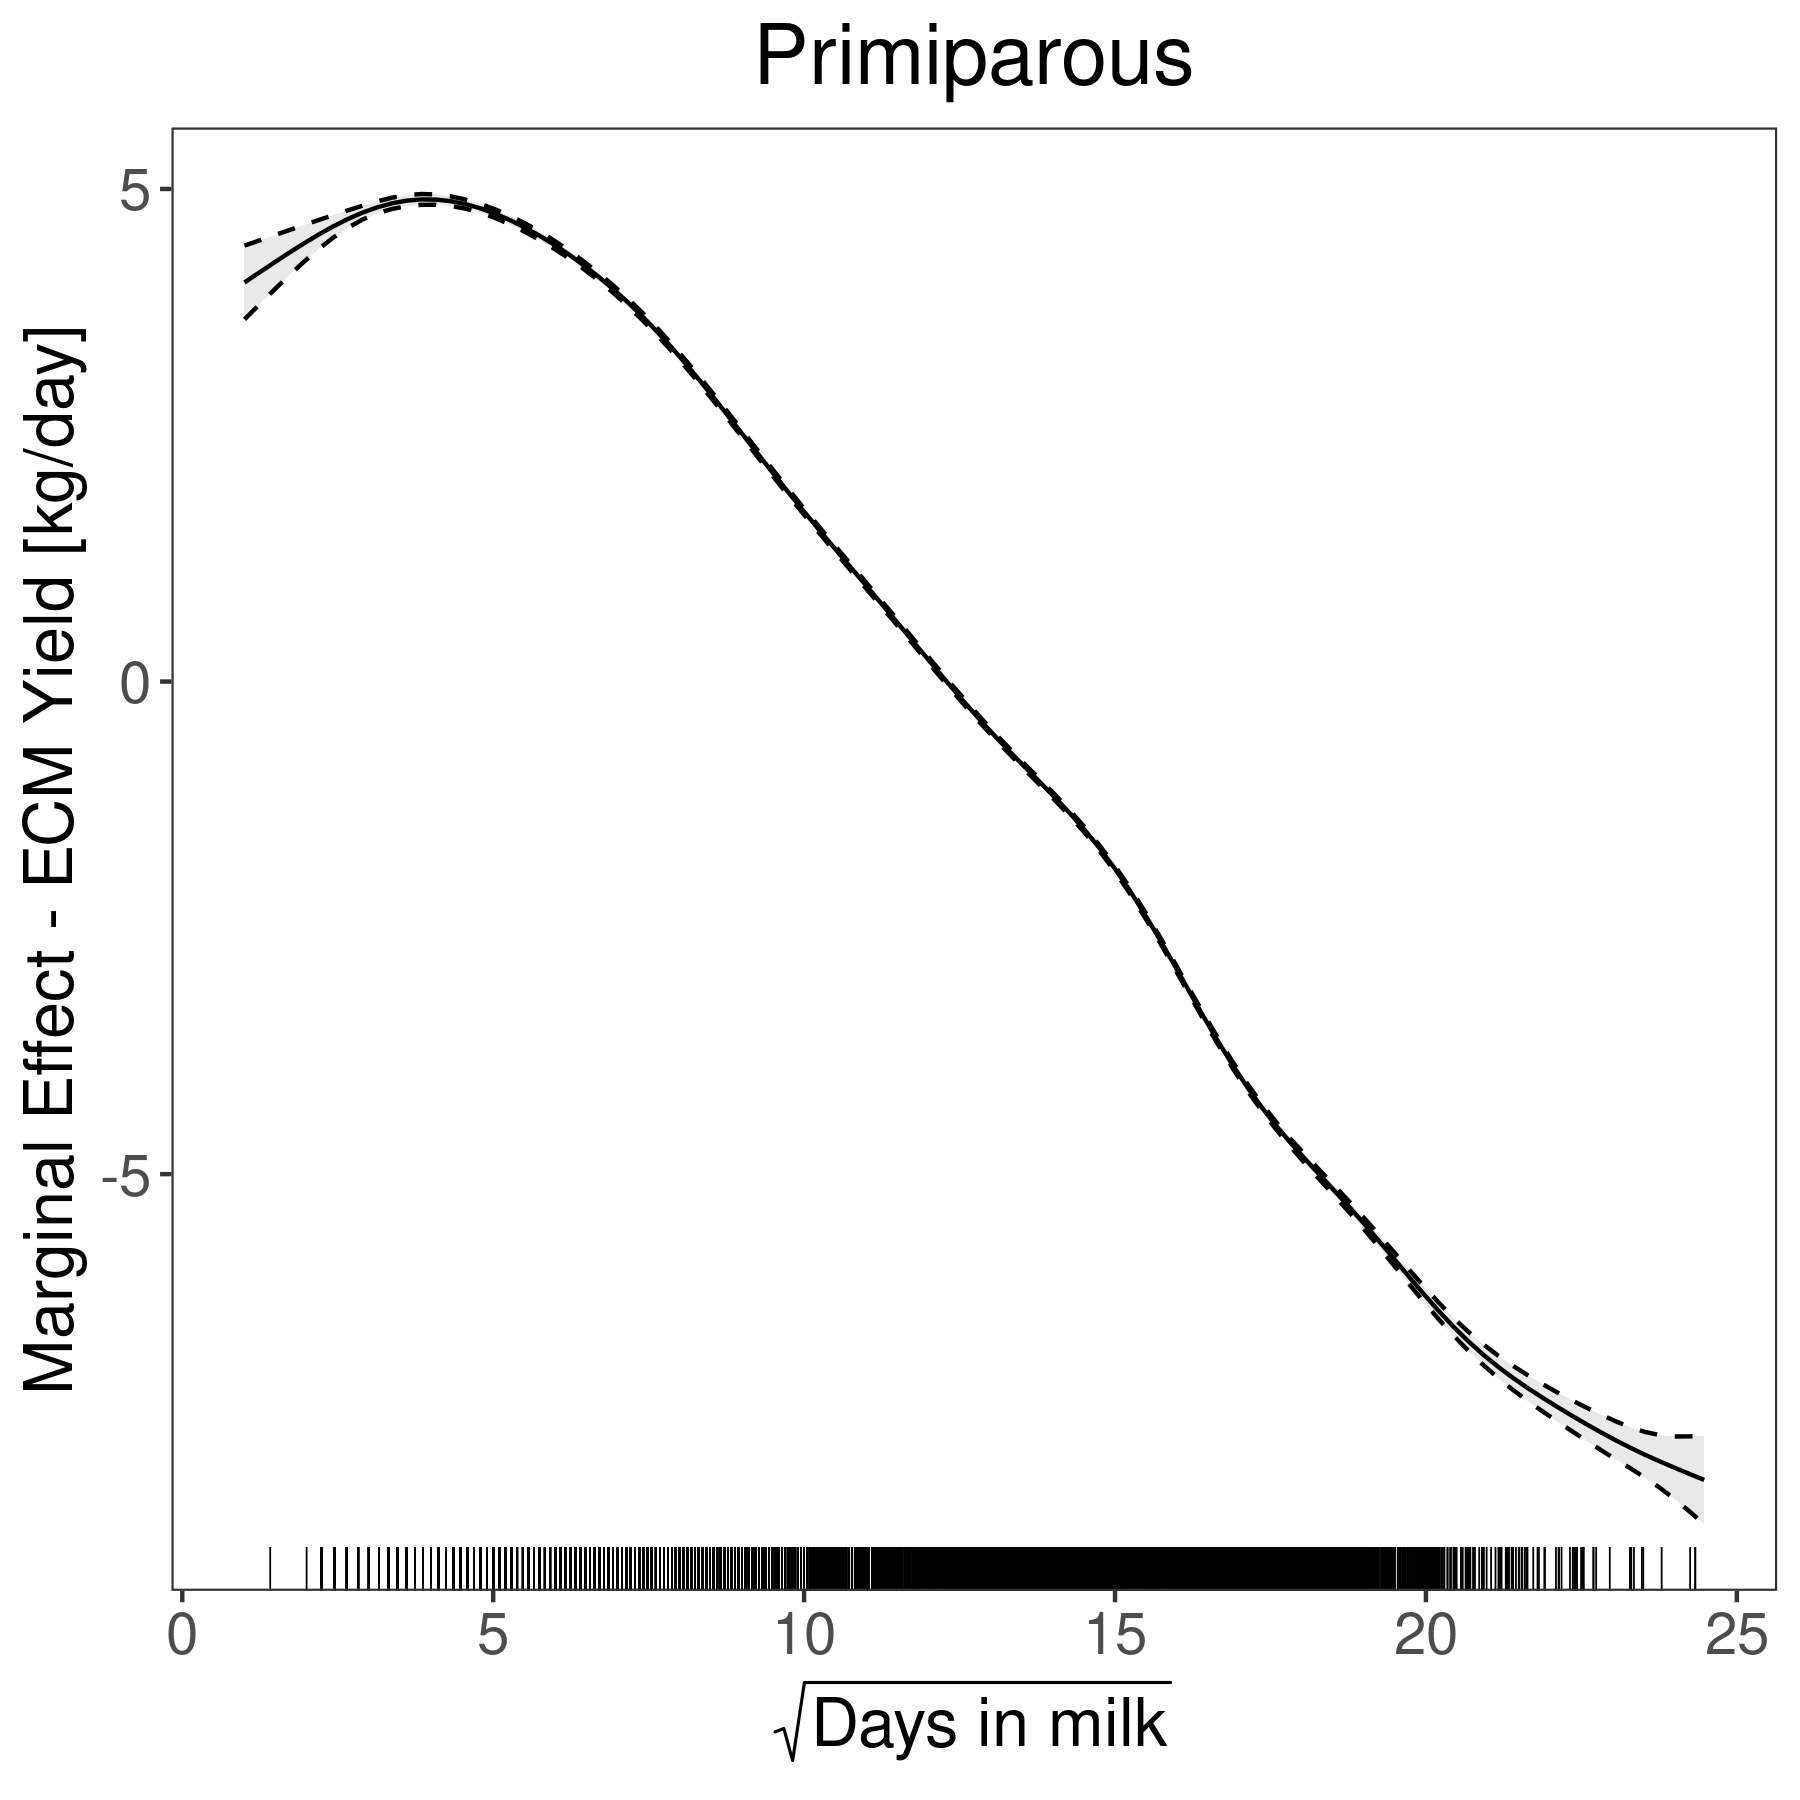
\includegraphics[width=\textwidth]{thesis/figures/models/ecm/before2010/ho_ecm_before2010/ho_ecm_before2010_marginal_dim_milk_primi.png}
    \end{subfigure}
    \begin{subfigure}[b]{0.45\textwidth}
        \centering
        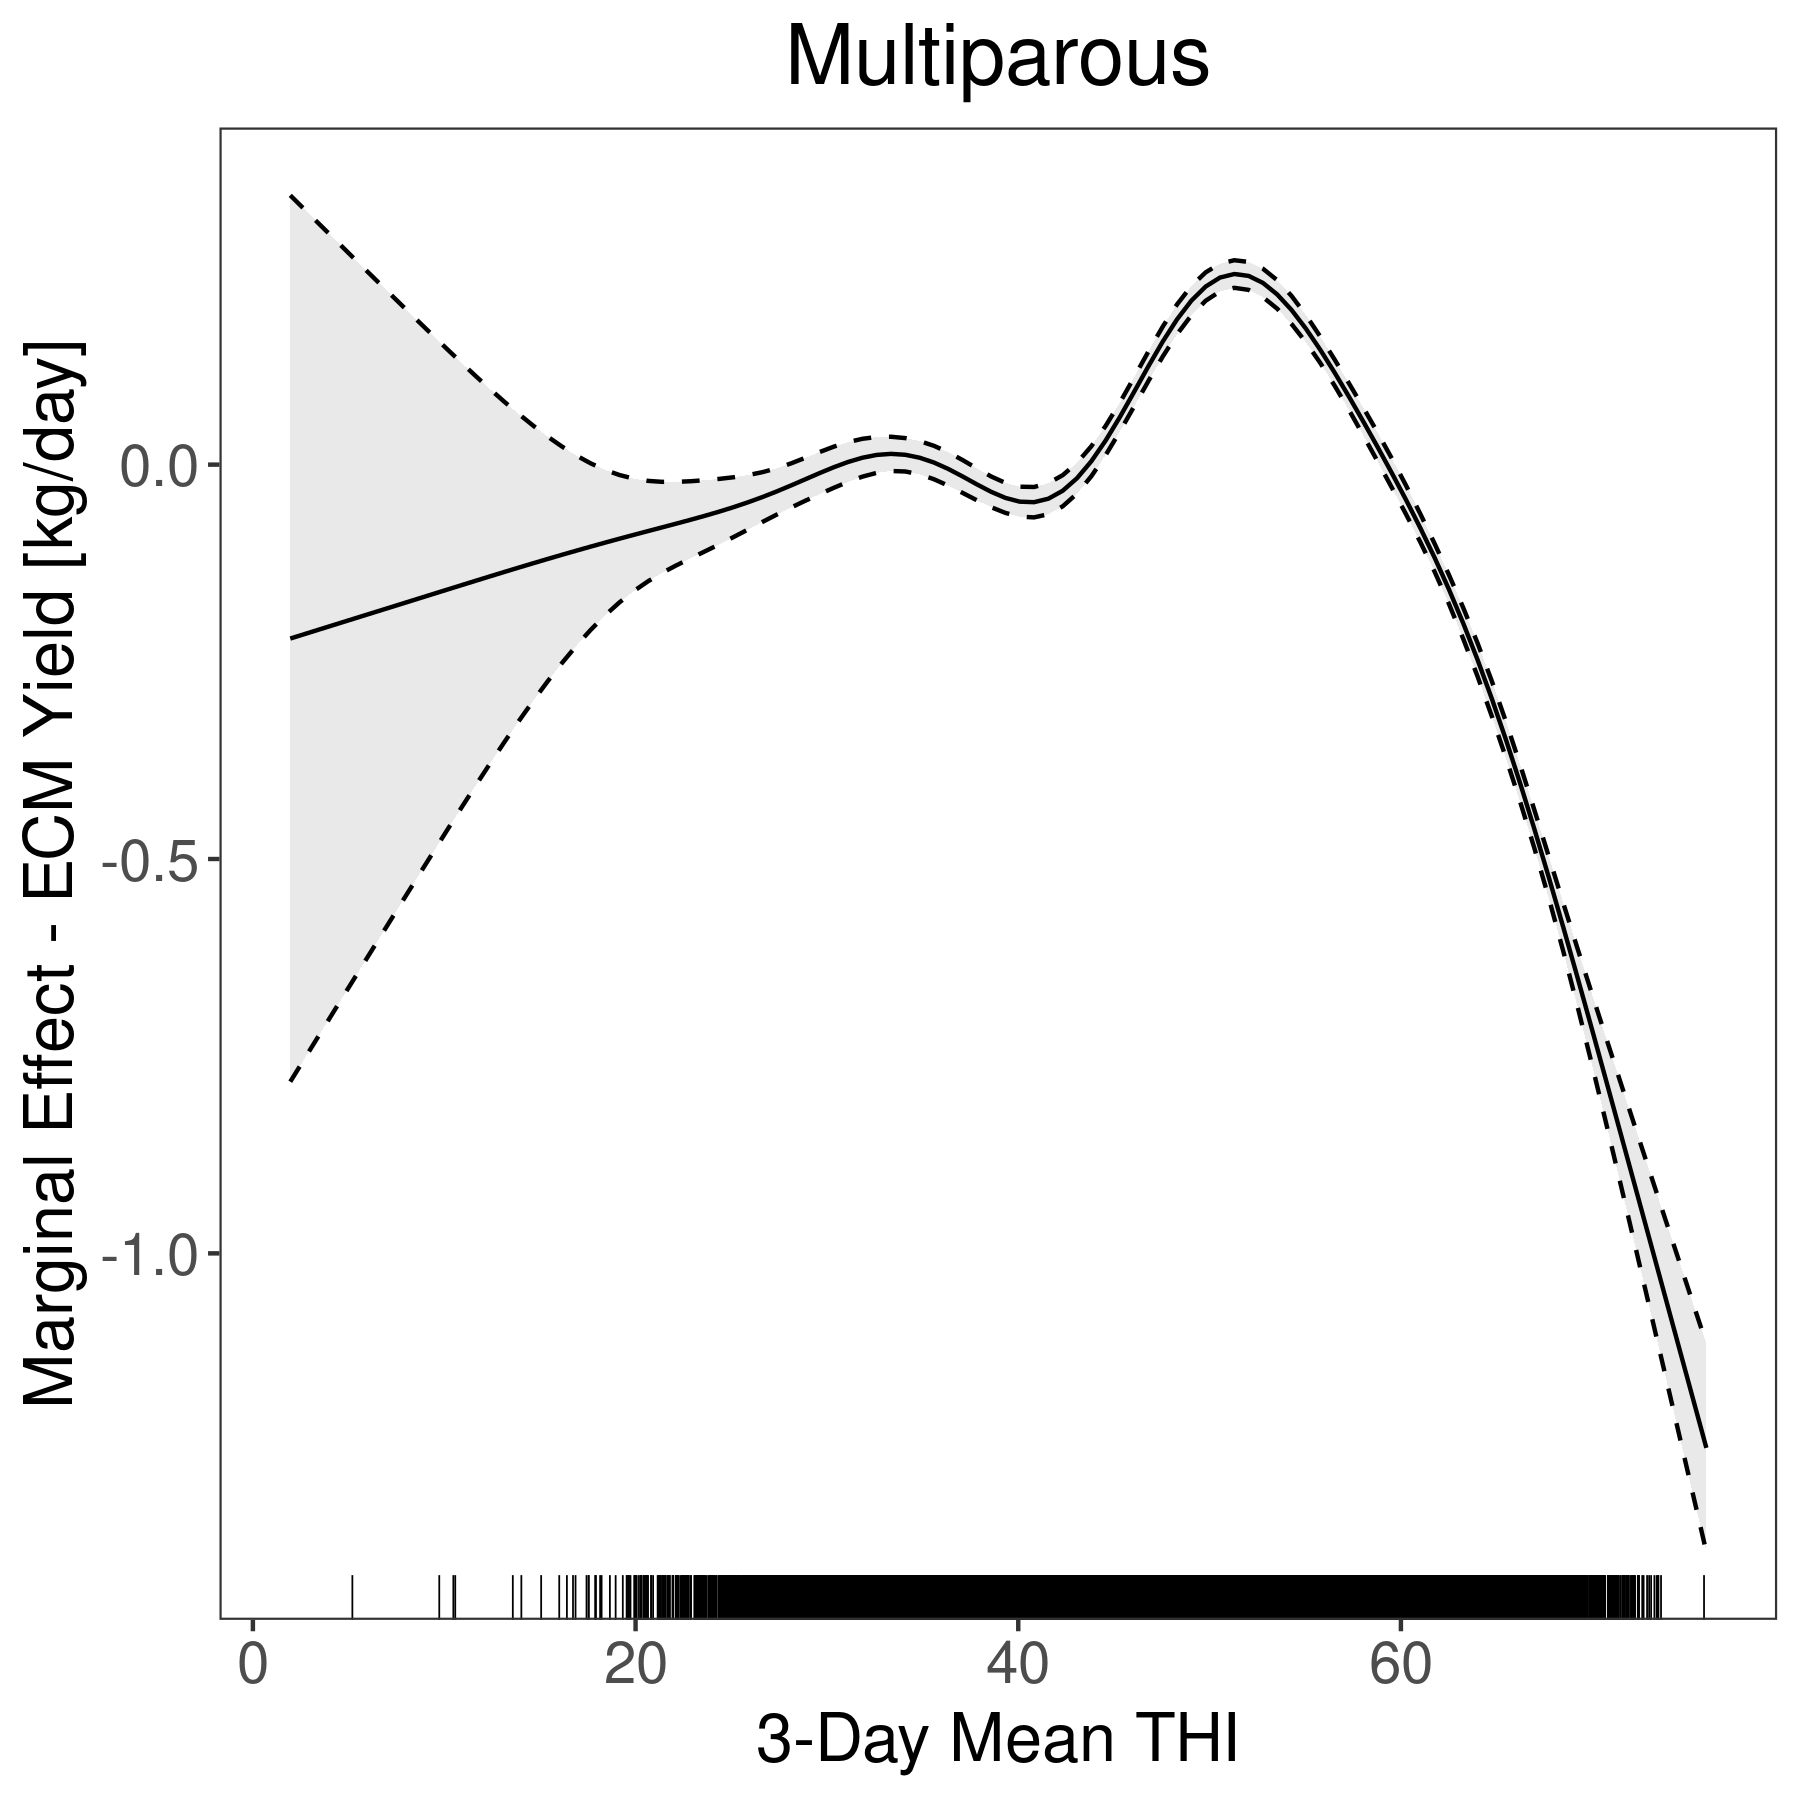
\includegraphics[width=\textwidth]{thesis/figures/models/ecm/before2010/ho_ecm_before2010/ho_ecm_before2010_marginal_thi_milk_multi.png}
    \end{subfigure}
    \hspace{0.05\textwidth} % Optional space between the figures
    \begin{subfigure}[b]{0.45\textwidth}
        \centering
        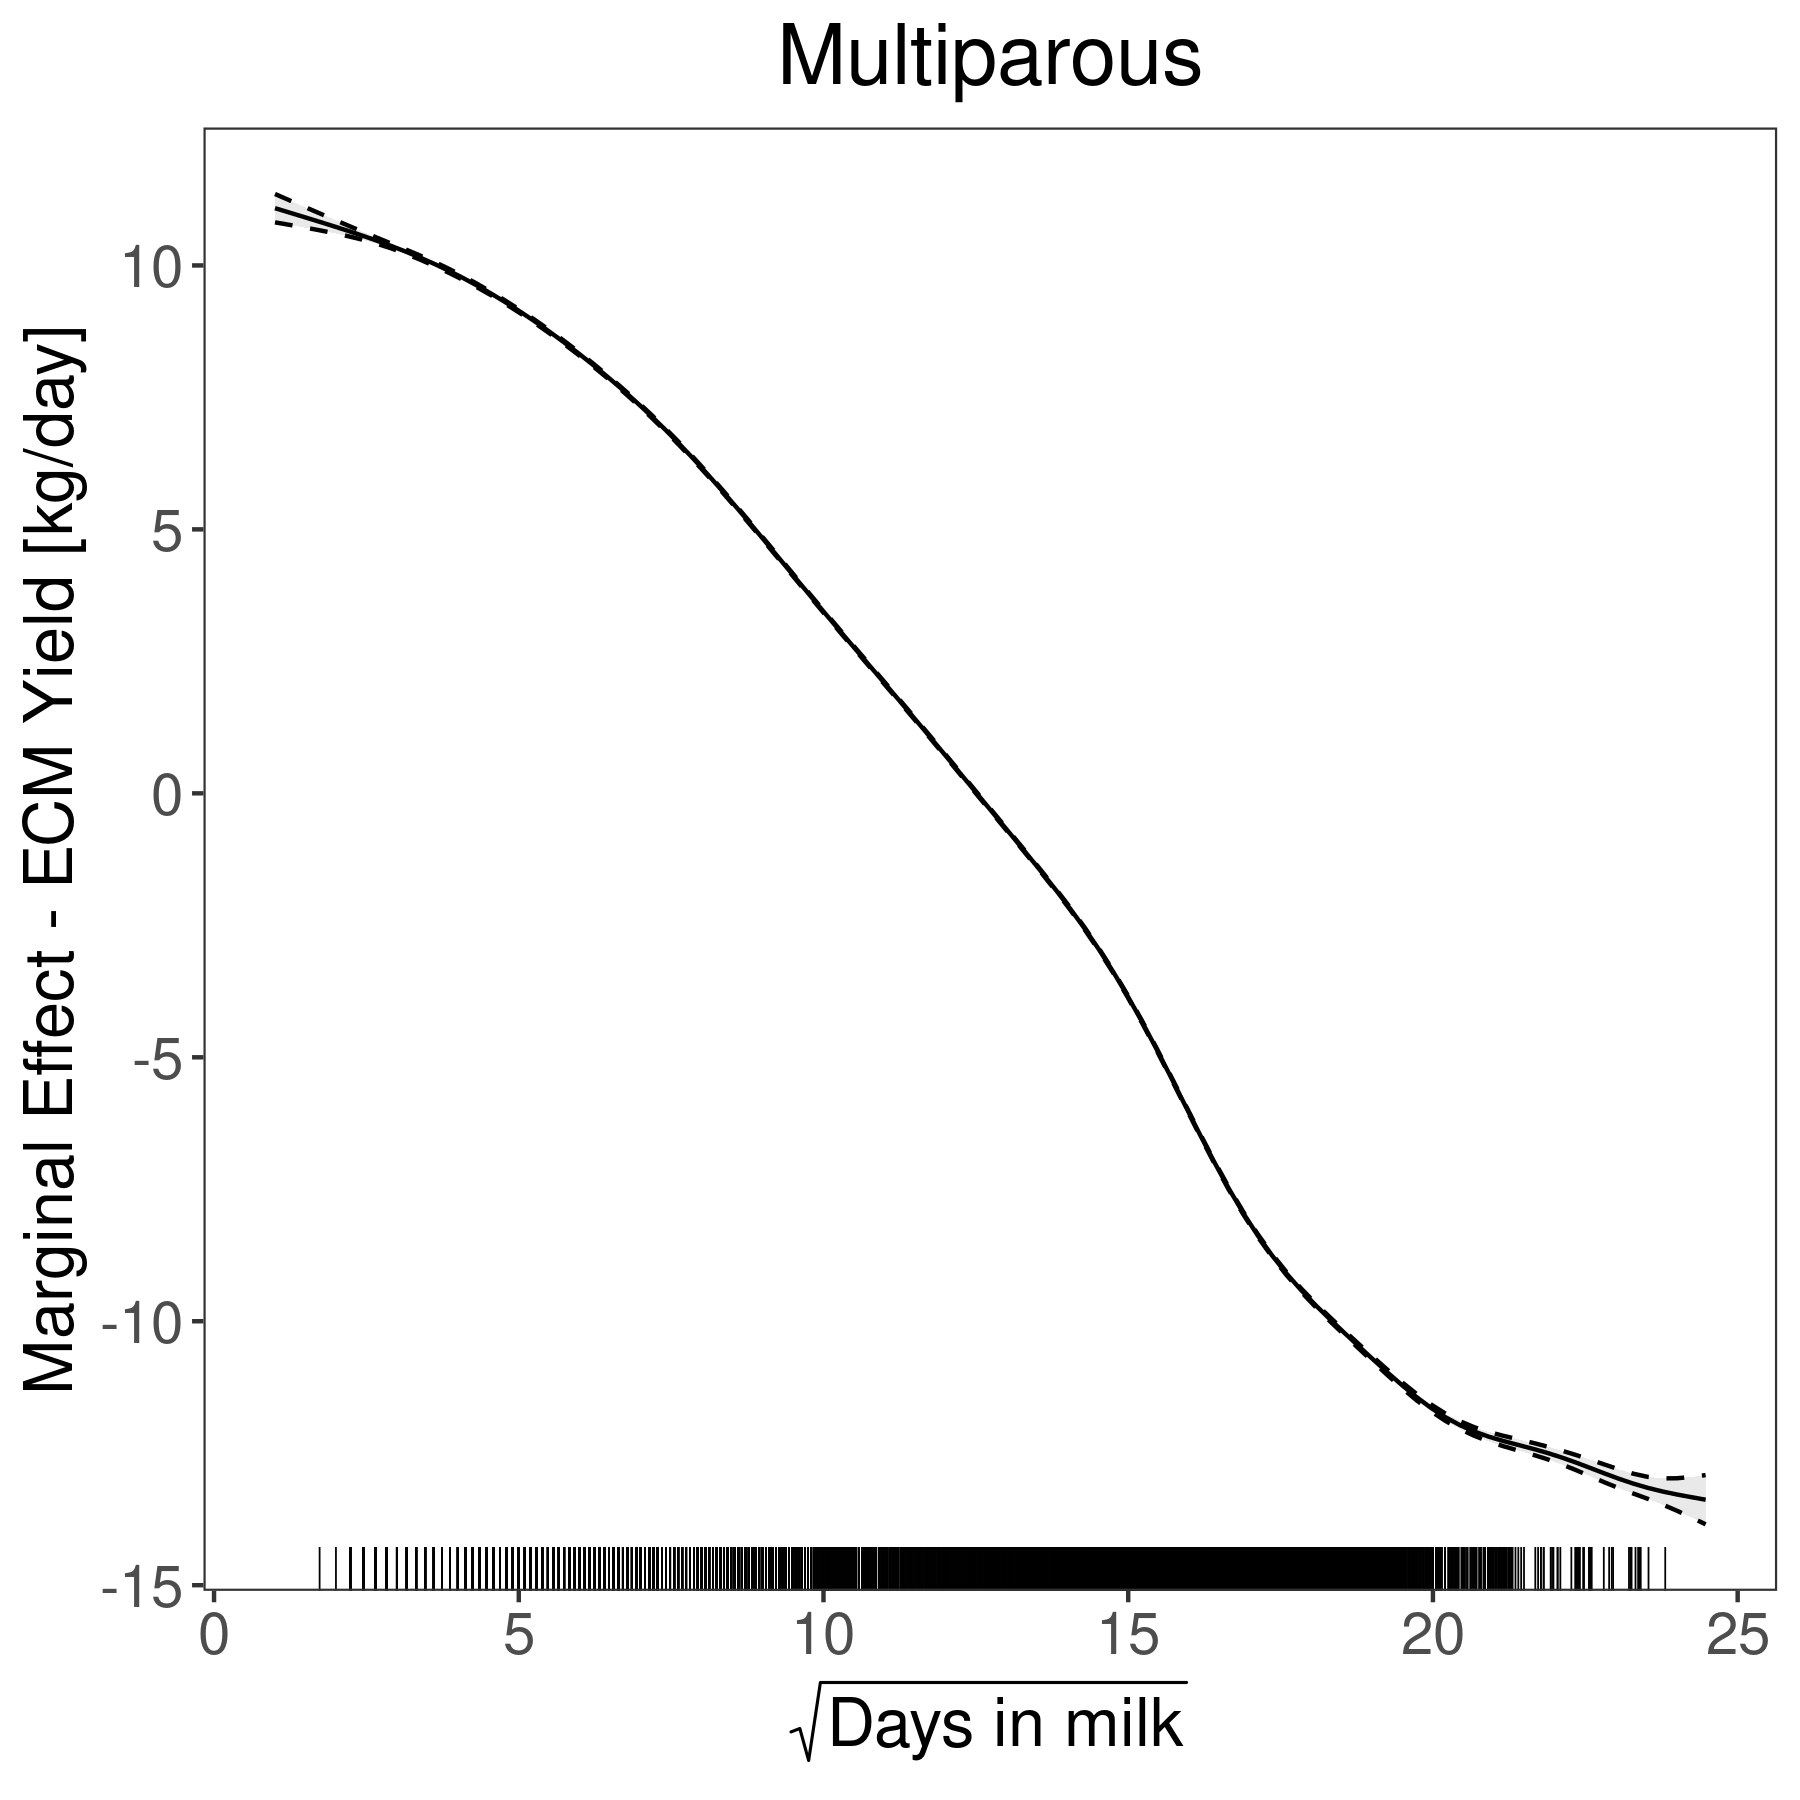
\includegraphics[width=\textwidth]{thesis/figures/models/ecm/before2010/ho_ecm_before2010/ho_ecm_before2010_marginal_dim_milk_multi.png}
    \end{subfigure}
    \caption[]{Holstein: ECM Yield - 1985 - 2010 - THI Effect and Lactation Curve}
    \label{fig:main}
\end{figure}

\subsubsection{Split Period: 2010 - 2023}\label{model:ho_ecm_after}

\paragraph{Model Summary} \quad \\

    \begin{table}[H]
    \centering
    \begin{tabular}{lrrrr}
    \textbf{A. parametric coefficients} & Estimate & Std. Error & t-value & p-value \\ 
       \hline
       \hline
  (Intercept) & 26.0912 & 0.3371 & 77.3959 & $<$ 0.0001 \\ 
  parityprimiparous & -4.1684 & 0.0144 & -289.2770 & $<$ 0.0001 \\ 
  year2012 & -0.0036 & 0.4530 & -0.0079 & 0.9937 \\ 
  year2013 & -0.4704 & 0.4087 & -1.1510 & 0.2497 \\ 
  year2014 & -0.0259 & 0.4077 & -0.0636 & 0.9493 \\ 
  year2015 & 0.3804 & 0.4236 & 0.8978 & 0.3693 \\ 
  year2016 & 0.7225 & 0.4482 & 1.6118 & 0.1070 \\ 
  year2017 & 1.0551 & 0.4375 & 2.4115 & 0.0159 \\ 
  year2018 & 1.7452 & 0.4307 & 4.0524 & 0.0001 \\ 
  year2019 & 1.9702 & 0.4251 & 4.6343 & $<$ 0.0001 \\ 
  year2020 & 2.6159 & 0.4280 & 6.1119 & $<$ 0.0001 \\ 
  year2021 & 2.8975 & 0.4212 & 6.8784 & $<$ 0.0001 \\ 
  year2022 & 2.6987 & 0.4087 & 6.6037 & $<$ 0.0001 \\ 
  year2023 & 3.2917 & 0.4105 & 8.0192 & $<$ 0.0001 \\
       \hline
    \textbf{B. smooth terms} & edf & Ref.df & F-value & p-value \\ 
    \hline
    \hline
  s(thi\_mean\_t0\_3d):paritymultiparous & 7.9522 & 7.9522 & 319.3654 & $<$ 0.0001 \\ 
  s(thi\_mean\_t0\_3d):parityprimiparous & 7.1992 & 7.1992 & 264.9658 & $<$ 0.0001 \\ 
  s(days\_in\_milk\_t):paritymultiparous & 13.6599 & 13.6599 & 103206.5817 & $<$ 0.0001 \\ 
  s(days\_in\_milk\_t):parityprimiparous & 12.7770 & 12.7770 & 7909.0701 & $<$ 0.0001 \\ 
       \hline
    \end{tabular}
    \caption[]{Holstein: ECM Yield - 2011-2023 - GAMM model summary without random effect terms.}
    \end{table}

\newpage
\begin{table}[H]
\centering
\begin{tabular}
{l | r | r | r | r}
\textbf{Smooth Term Fixed Effect} & Est. & SE & z & p\\
\hline
\hline
s(thi\_mean\_t0\_3d):multiFx1 & 0.6969 & 0.1034 & 6.74 & $<$ 1e-10 \\
s(thi\_mean\_t0\_3d):primiFx1 & 0.6876 & 0.1398 & 4.92 & $<$ 1e-06 \\
s(days\_in\_milk\_):multiFx1 & 2.6534 & 0.4168 & 6.37 & $<$ 1e-09 \\
s(days\_in\_milk\_):primiFx1 & 2.1363 & 0.4968 & 4.30 & $<$ 1e-04\\
\hline
\textbf{Variance Component} & Estimated $\sigma$ & & & \\
\hline
\hline
$\sigma_\alpha$ & 3.1148 & &  & \\
$\sigma_\iota$ & 1.2275 & & & \\
$\sigma_\phi$ & 4.1812 & & & \\
s(thi\_mean\_t0\_3d):multi & 1.7213 & & & \\
s(days\_in\_milk\_):primi & 5.7506 & & & \\
s(days\_in\_milk\_):multi & 8.9112 & & & \\
s(thi\_mean\_t0\_3d):primi & 1.7948 & & & \\
Residual & 4.3794 & & & \\
\end{tabular}
\caption[]{Holstein: ECM Yield - 2011-2023 - Mixed Model Summary - Smooth Terms and Random Effects.}
\end{table}


\paragraph{Model Diagnostics} \quad \\
\begin{figure}[H]
    \centering
    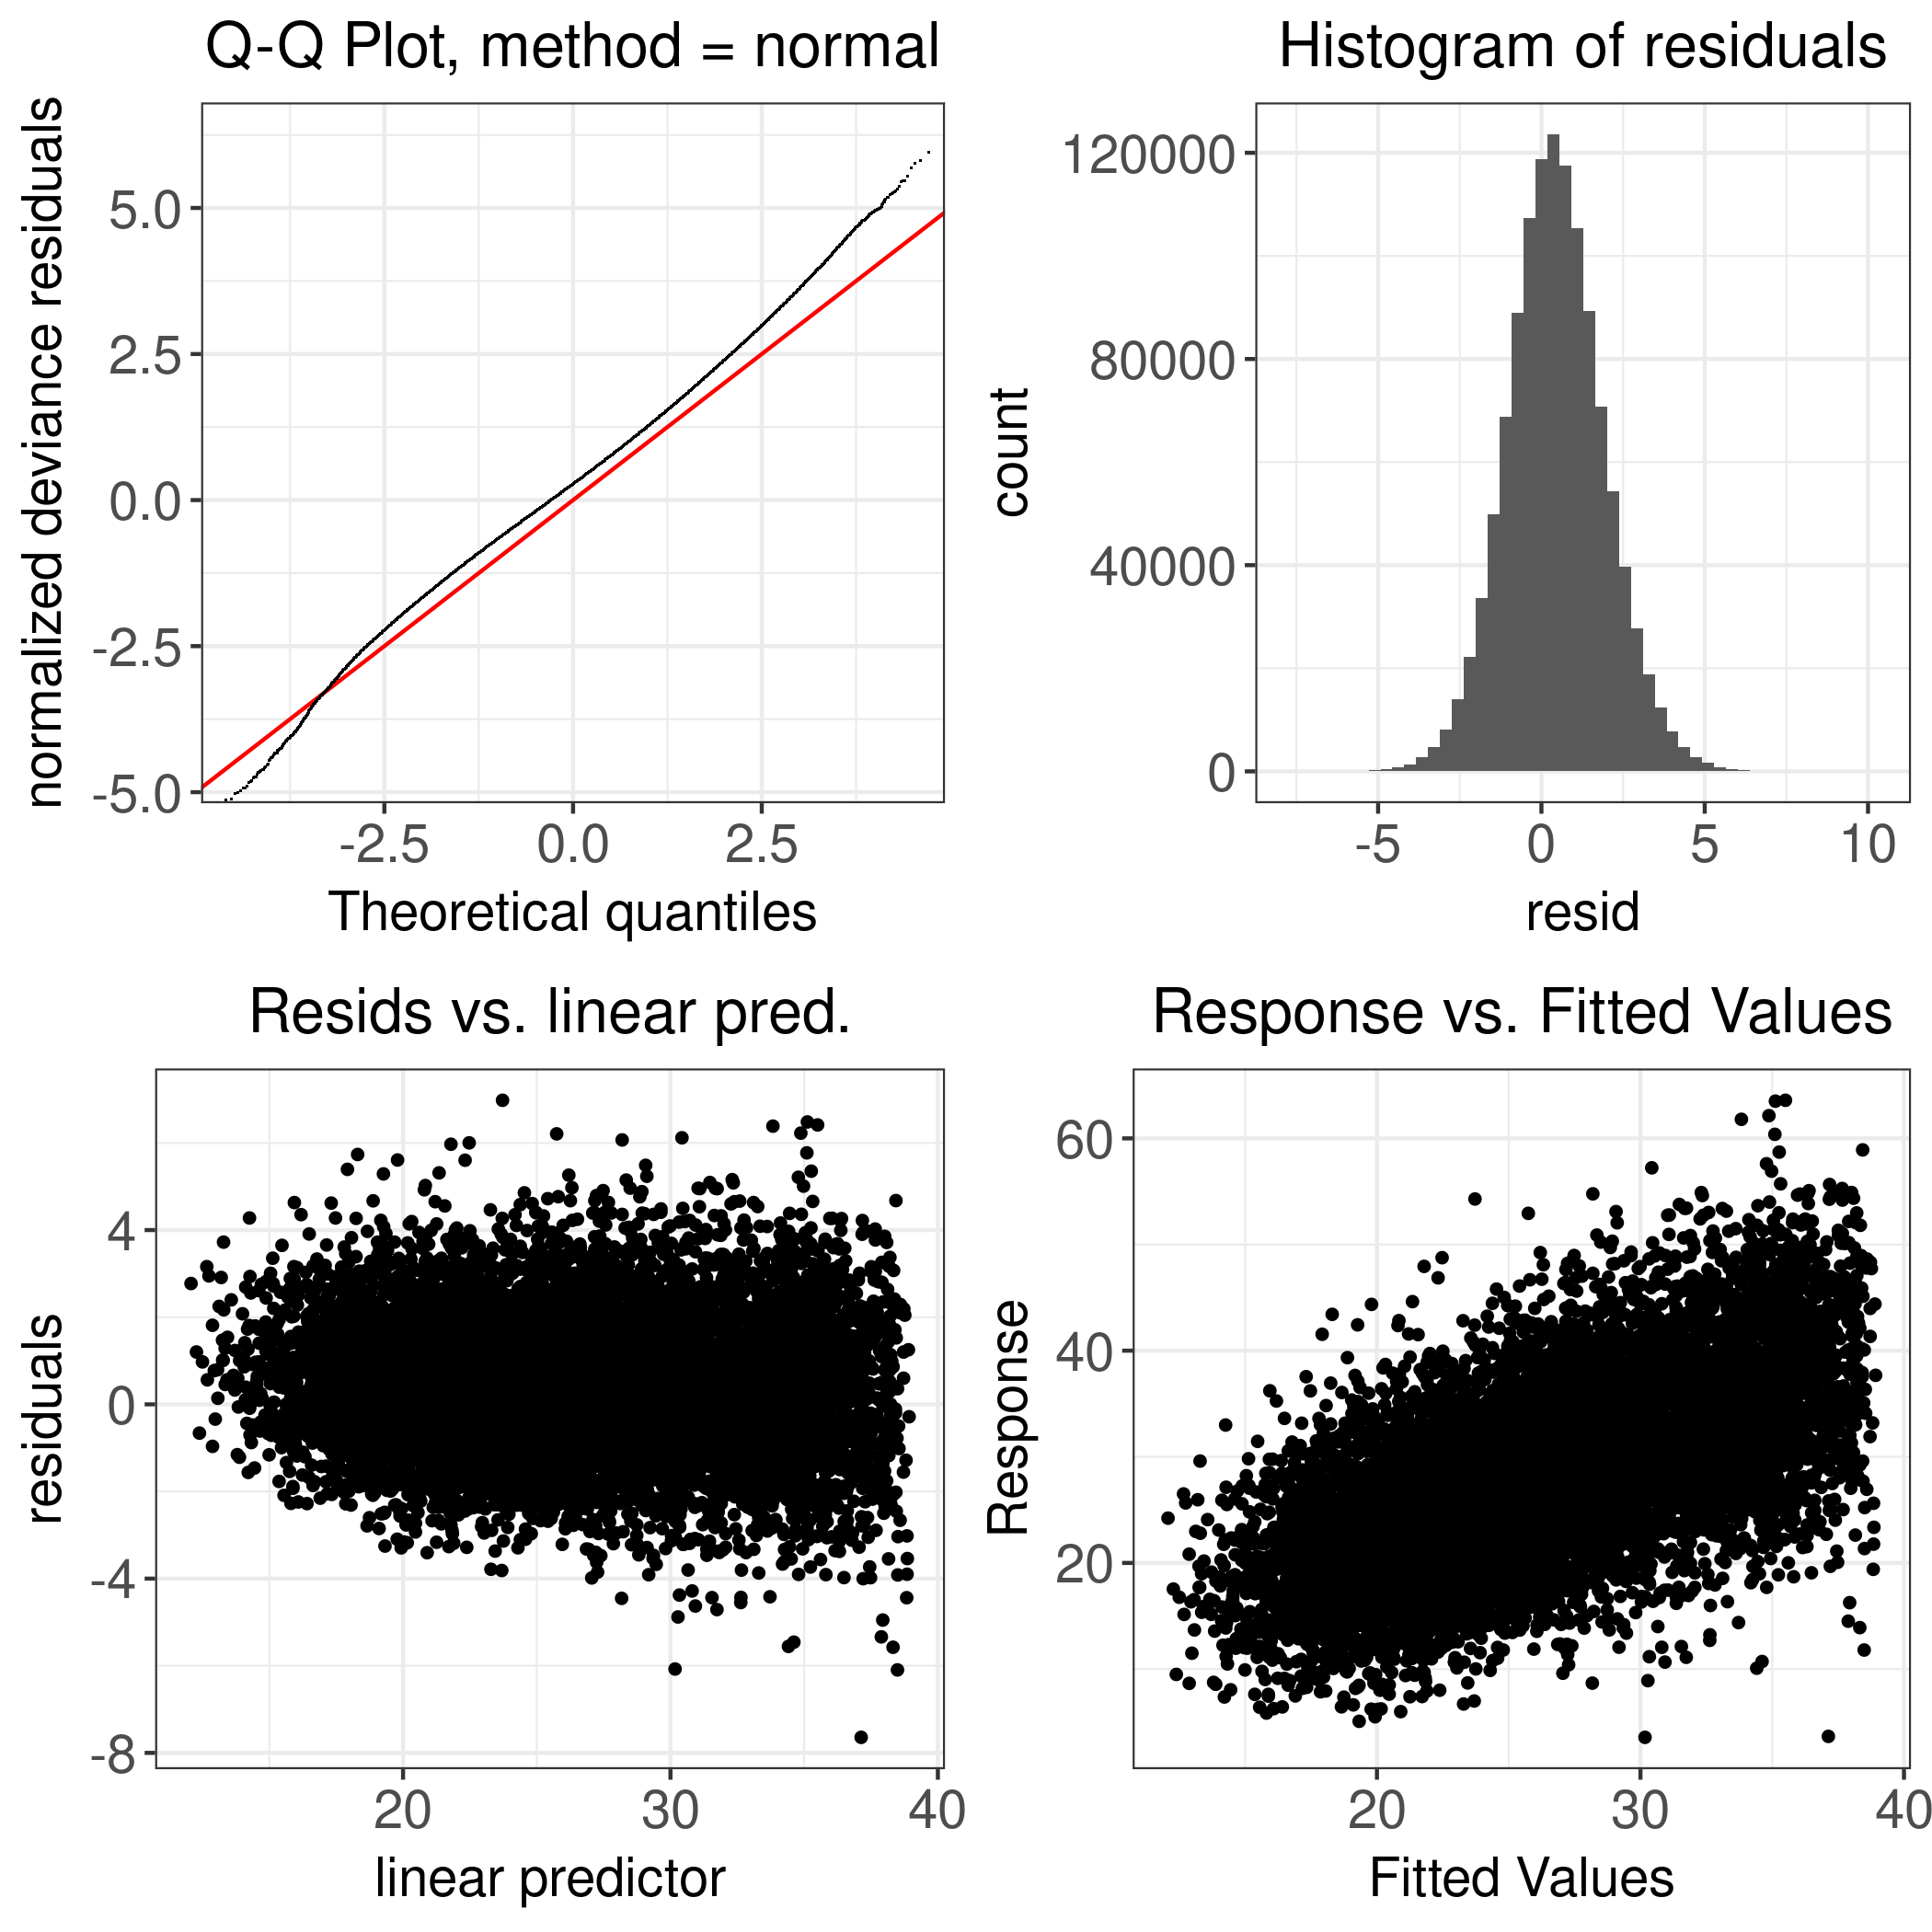
\includegraphics[width=0.6\textwidth]{thesis/figures/models/ecm/after2010/ho_ecm_after2010/ho_ecm_after2010_diagnostics.png}
    \caption[]{Holstein: ECM Yield - 2011 - 2023 - Diagnostic Plot}
\end{figure}

\newpage
\paragraph{THI Effect and Lactation Curve} \quad \\
\begin{figure}[H]
    \centering
    \begin{subfigure}[b]{0.45\textwidth}
        \centering
        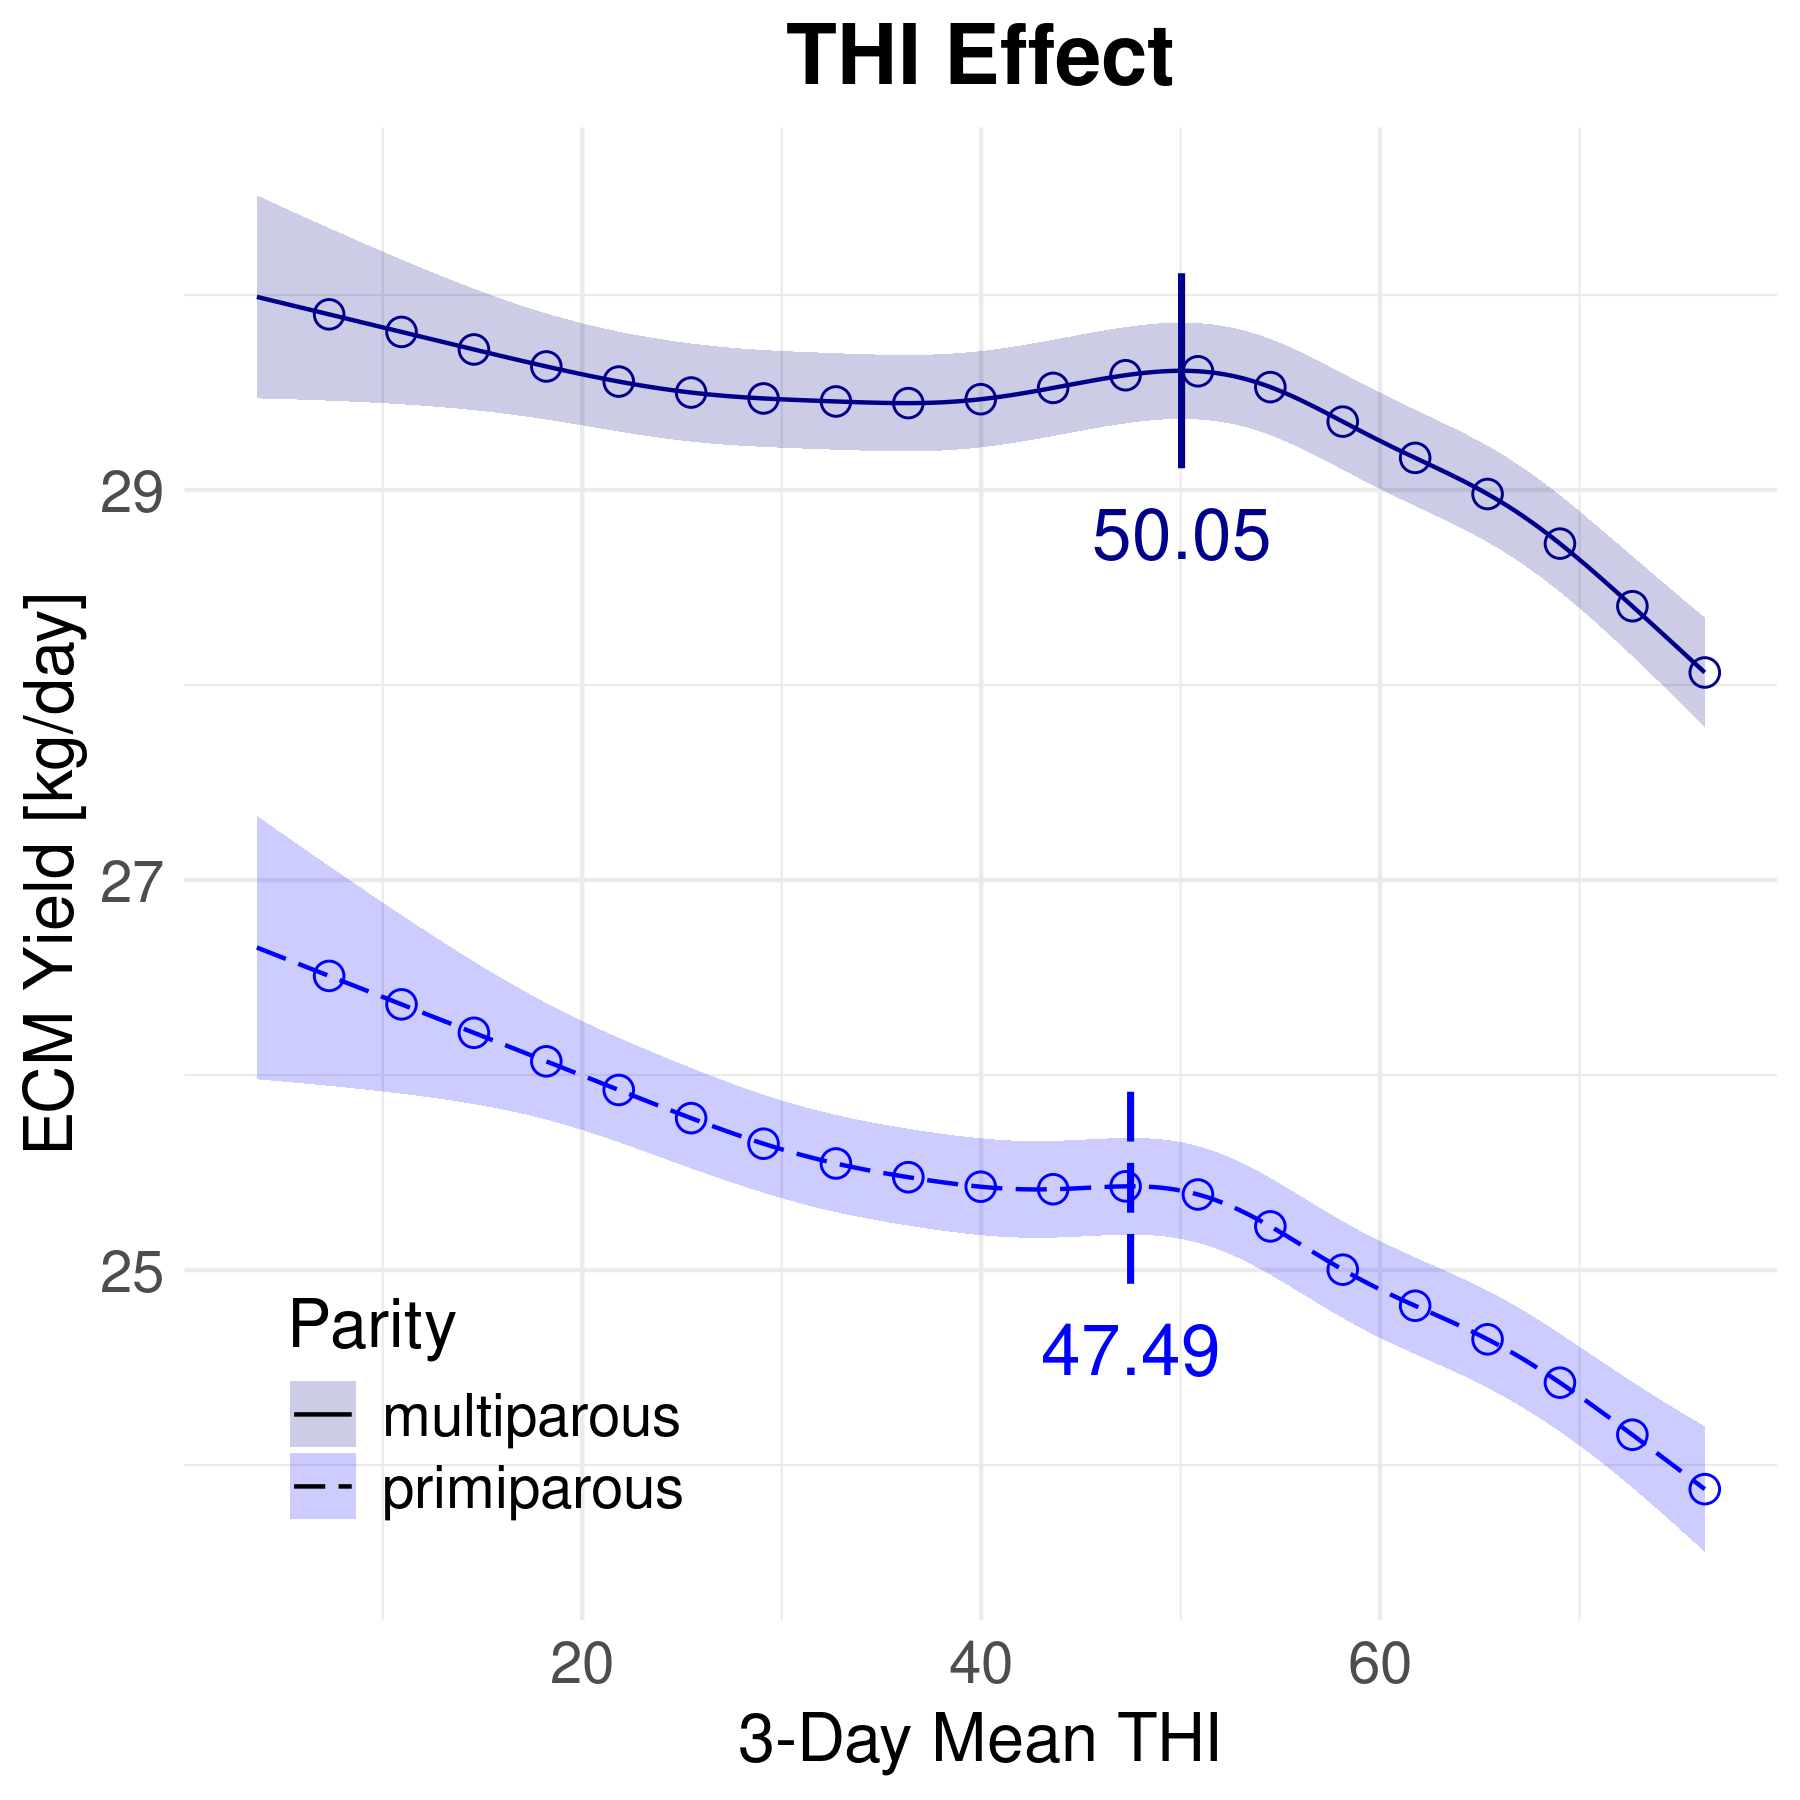
\includegraphics[width=\textwidth]{thesis/figures/models/ecm/after2010/ho_ecm_after2010/ho_ecm_after2010_marginal_thi_milk_combined.png}
    \end{subfigure}
    \hspace{0.05\textwidth} % Optional space between the figures
    \begin{subfigure}[b]{0.45\textwidth}
        \centering
        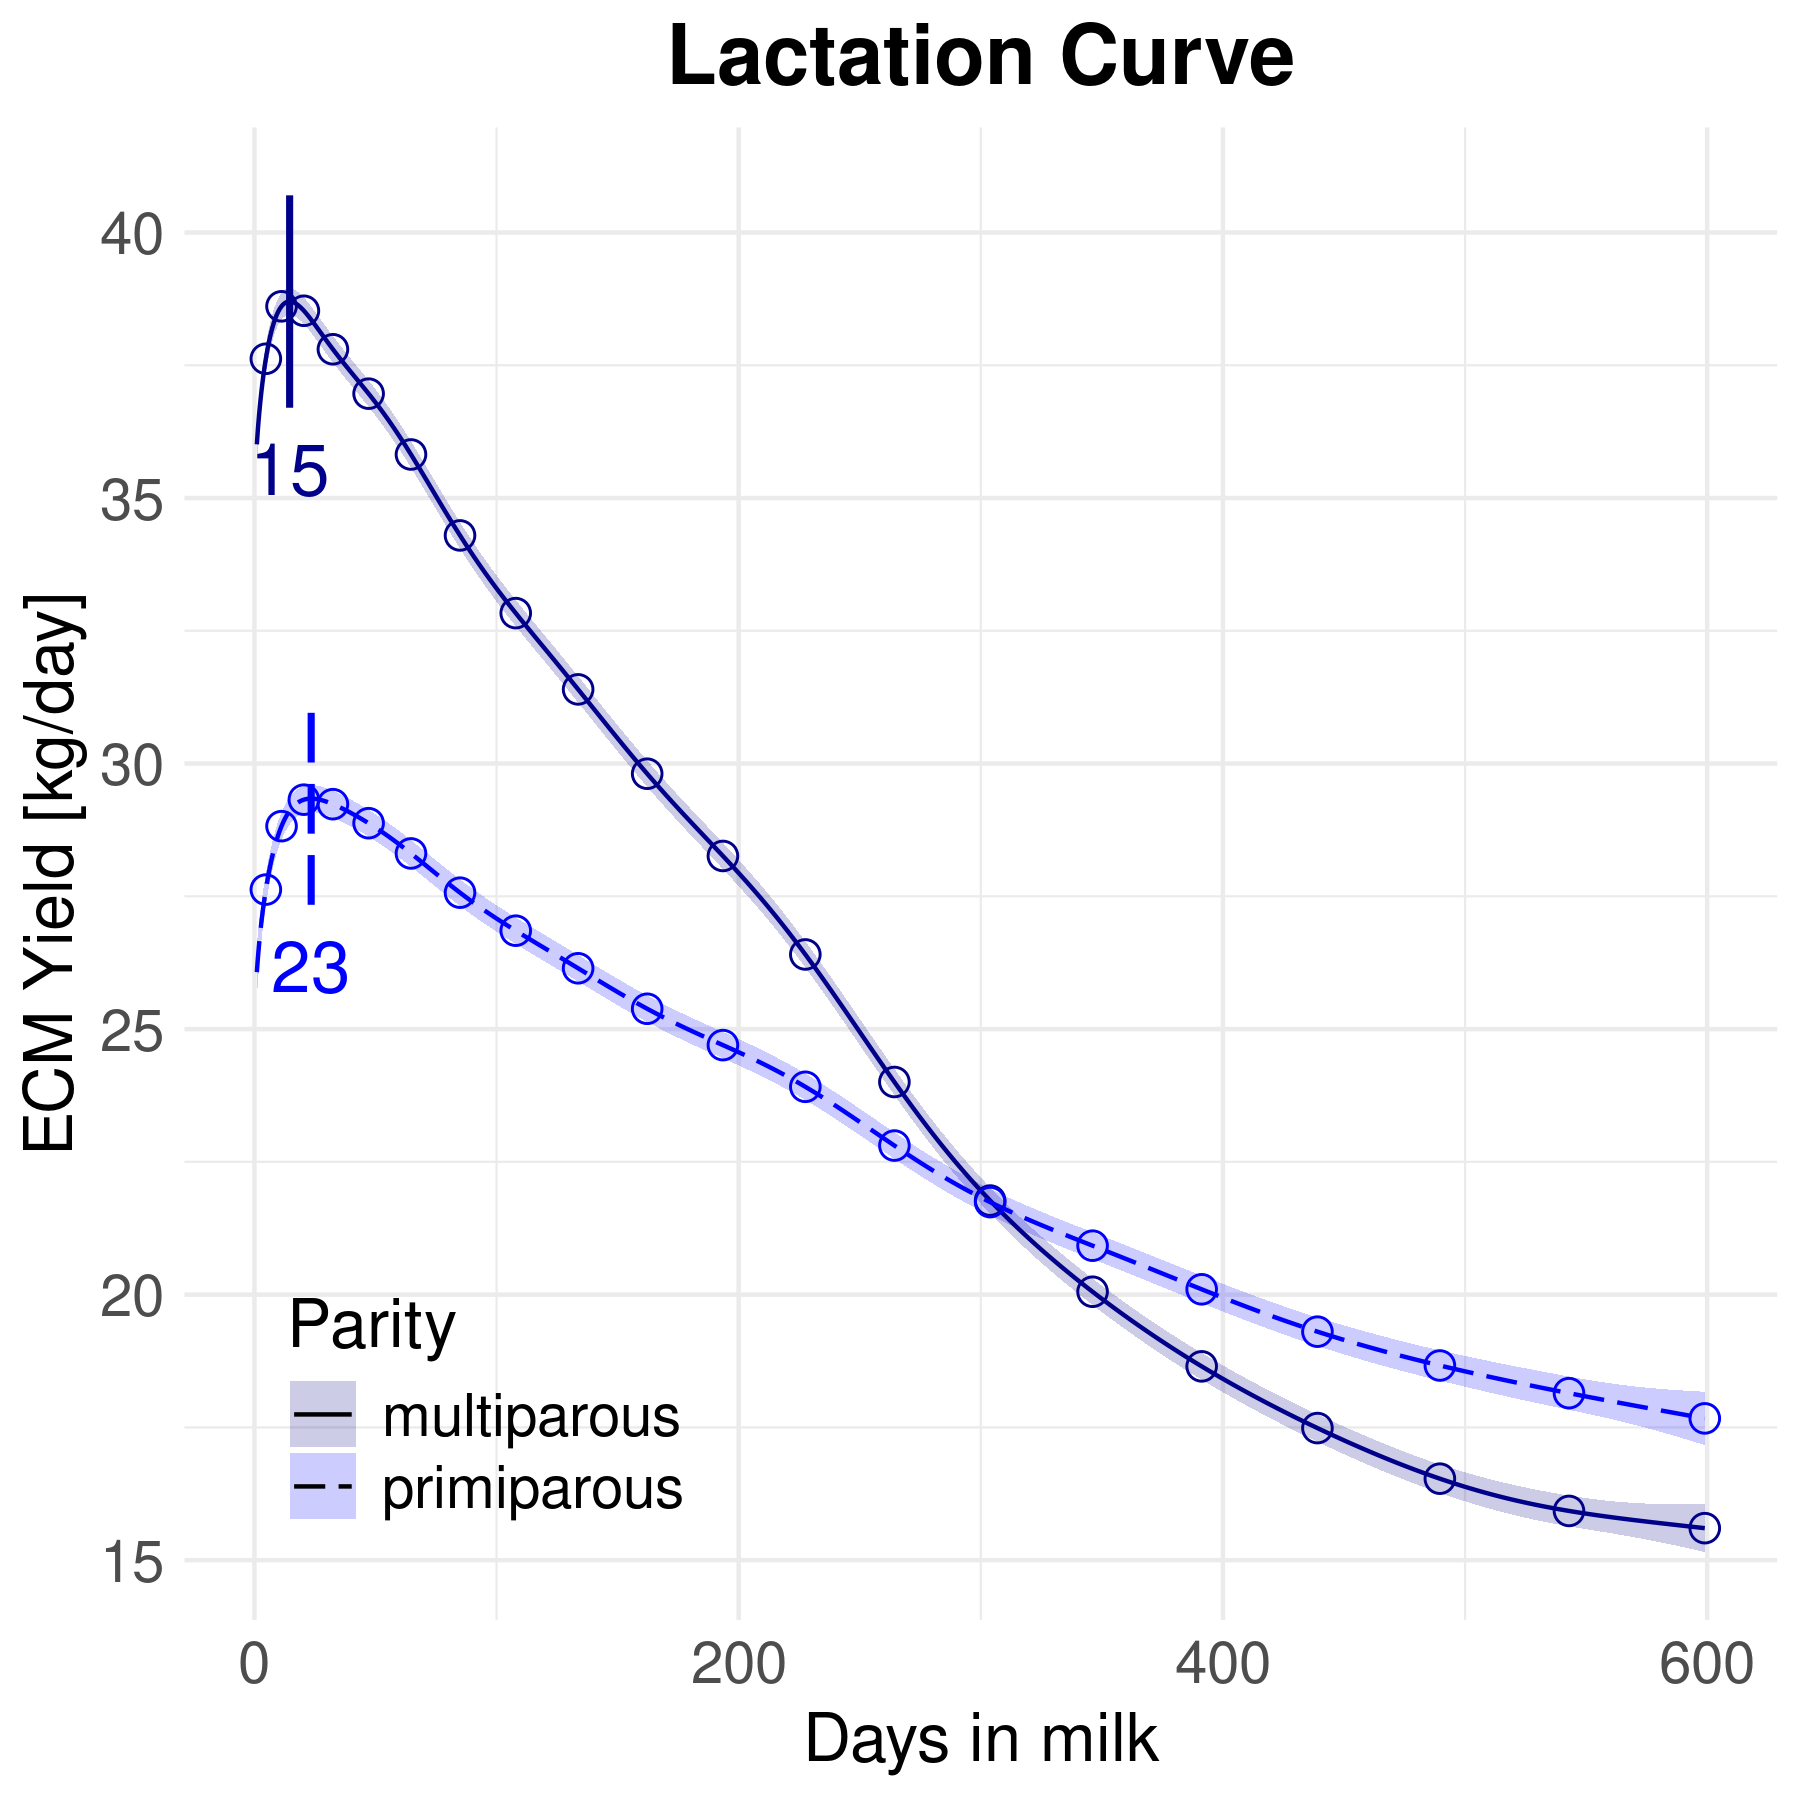
\includegraphics[width=\textwidth]{thesis/figures/models/ecm/after2010/ho_ecm_after2010/ho_ecm_after2010_marginal_dim_milk_combined.png}
    \end{subfigure}
    \begin{subfigure}[b]{0.45\textwidth}
        \centering
        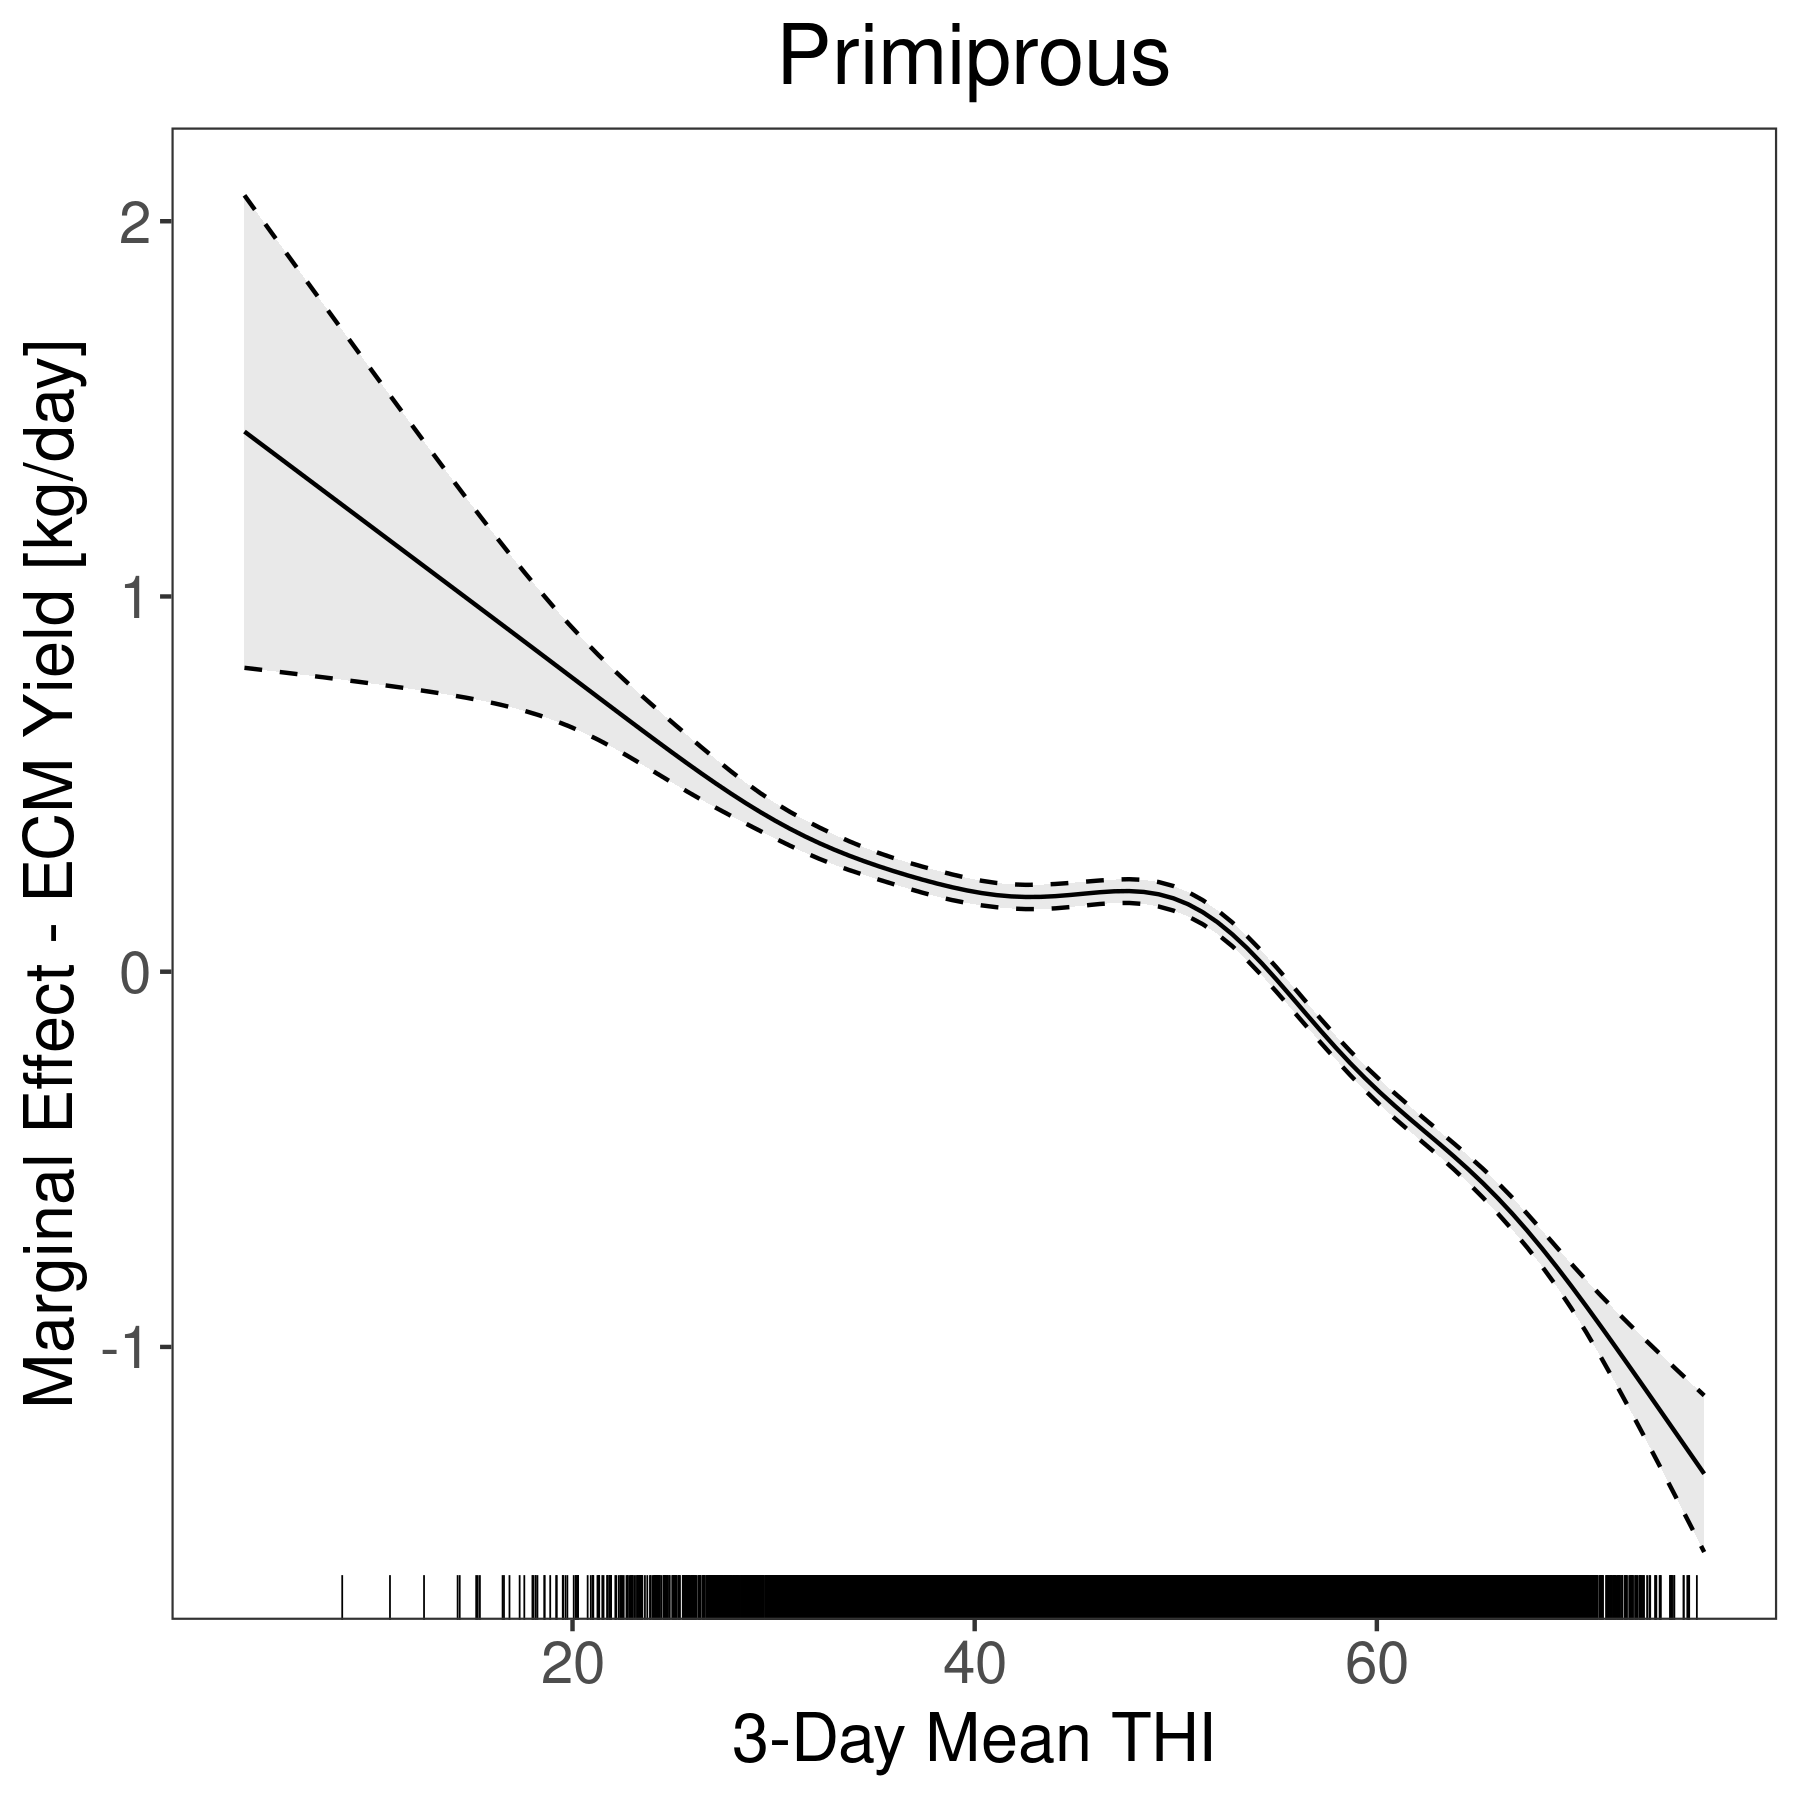
\includegraphics[width=\textwidth]{thesis/figures/models/ecm/after2010/ho_ecm_after2010/ho_ecm_after2010_marginal_thi_milk_primi.png}
    \end{subfigure}
    \hspace{0.05\textwidth} % Optional space between the figures
    \begin{subfigure}[b]{0.45\textwidth}
        \centering
        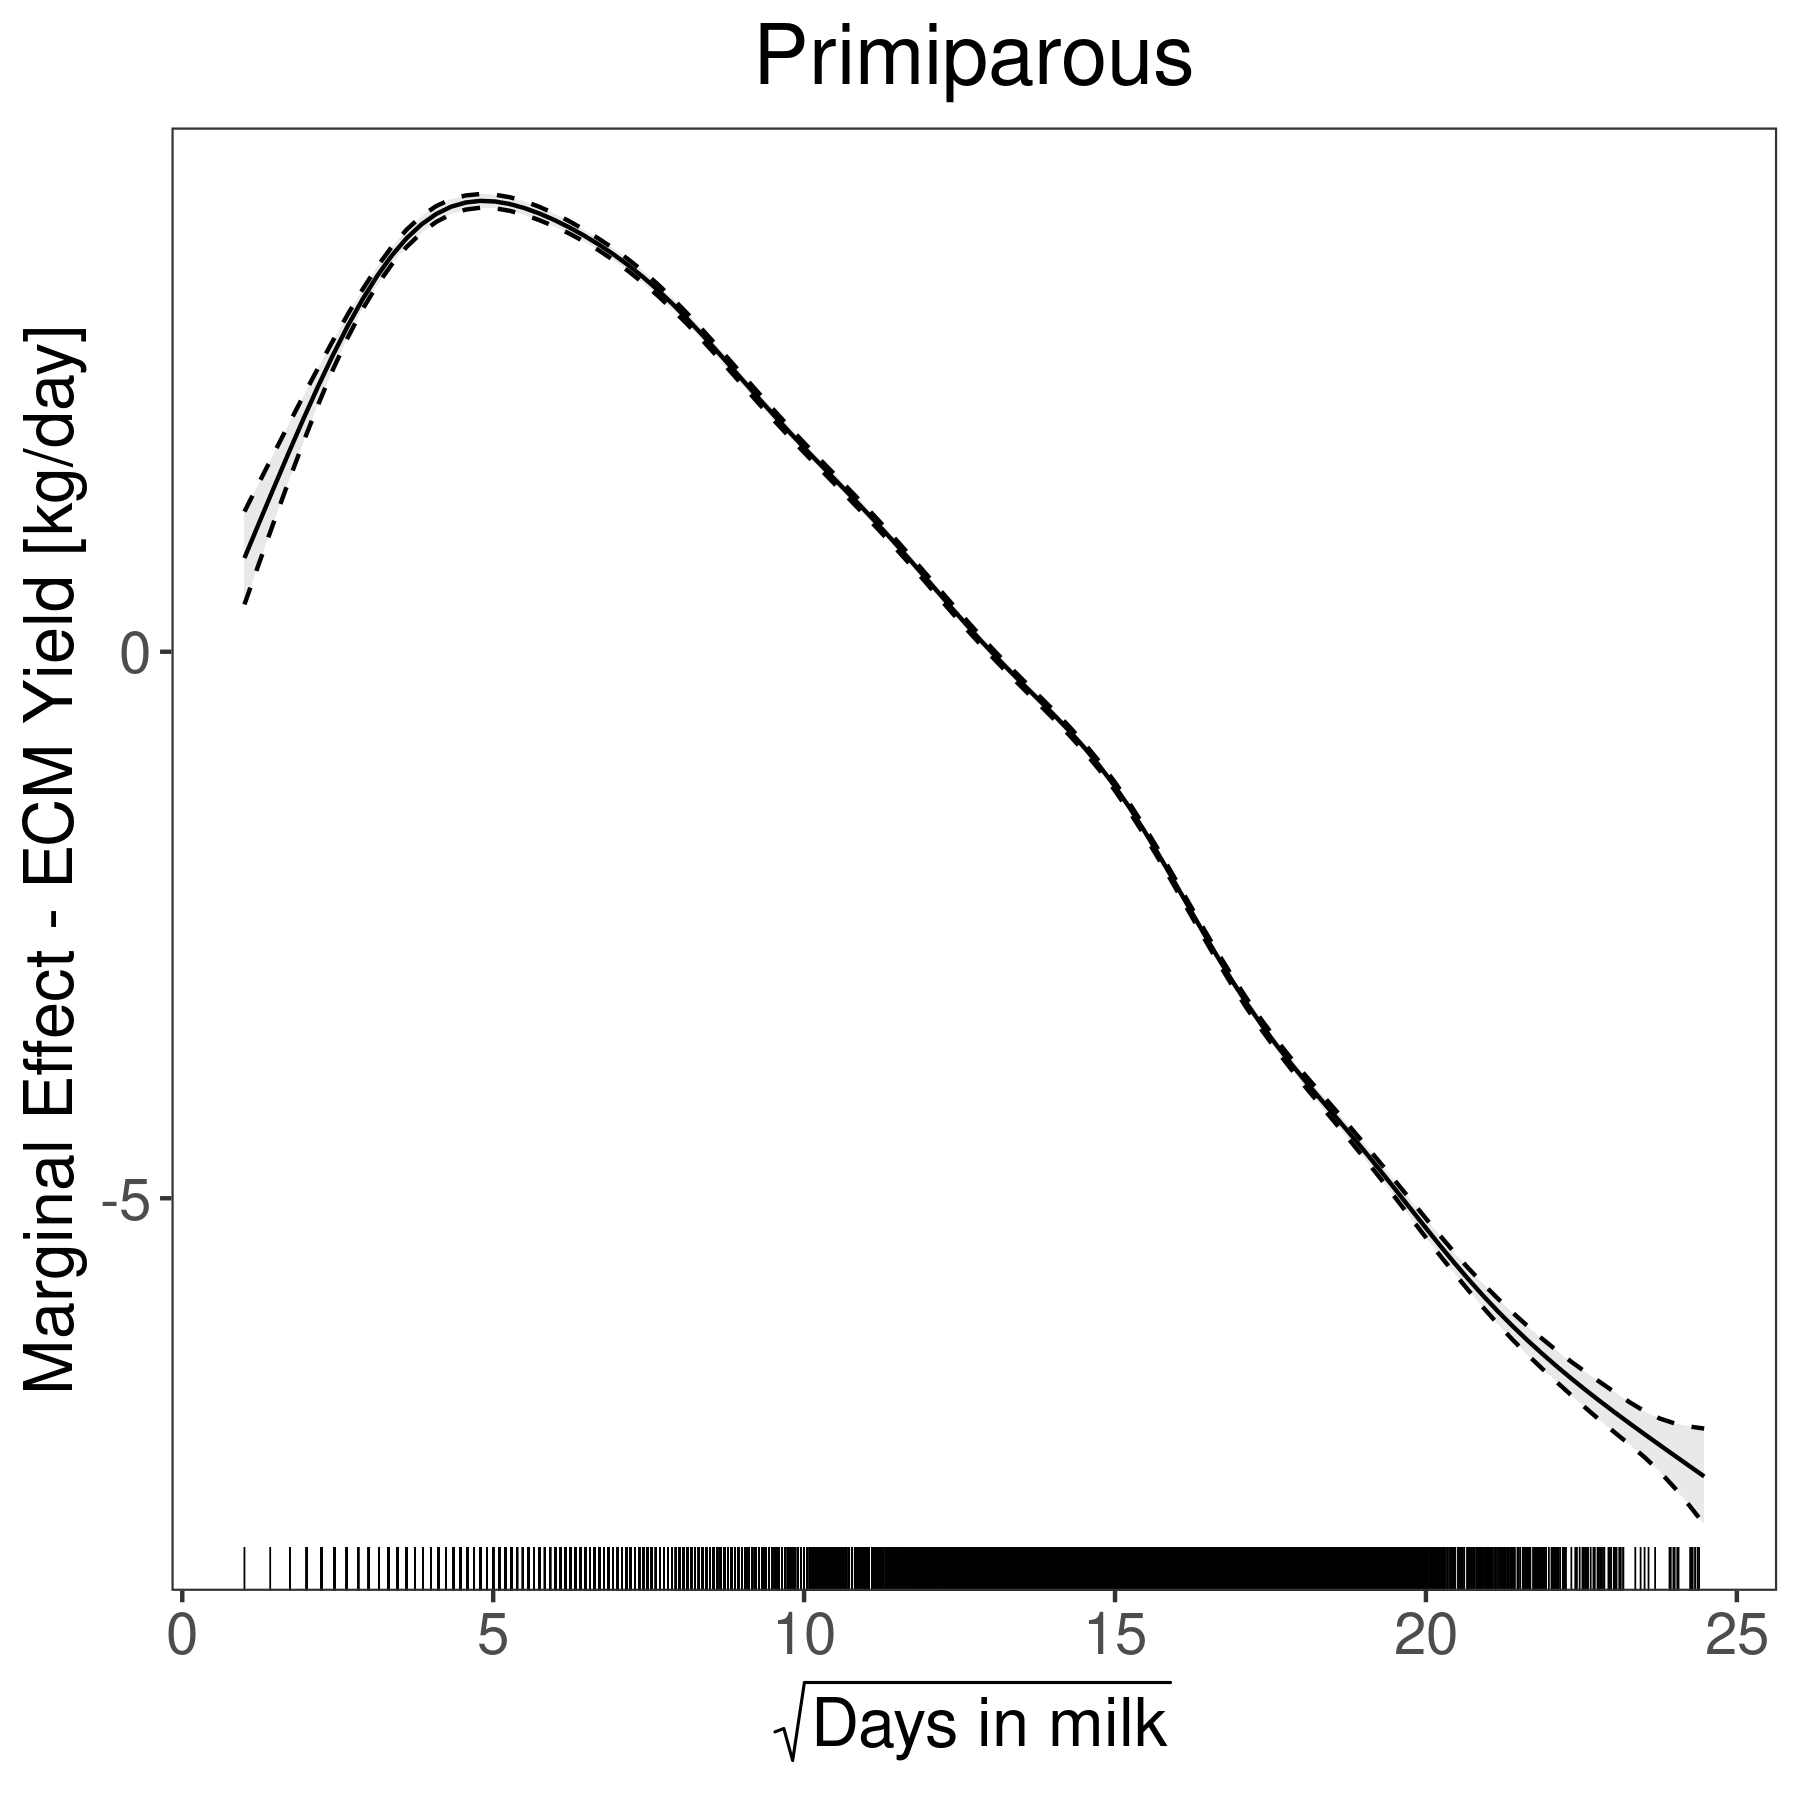
\includegraphics[width=\textwidth]{thesis/figures/models/ecm/after2010/ho_ecm_after2010/ho_ecm_after2010_marginal_dim_milk_primi.png}
    \end{subfigure}
    \begin{subfigure}[b]{0.45\textwidth}
        \centering
        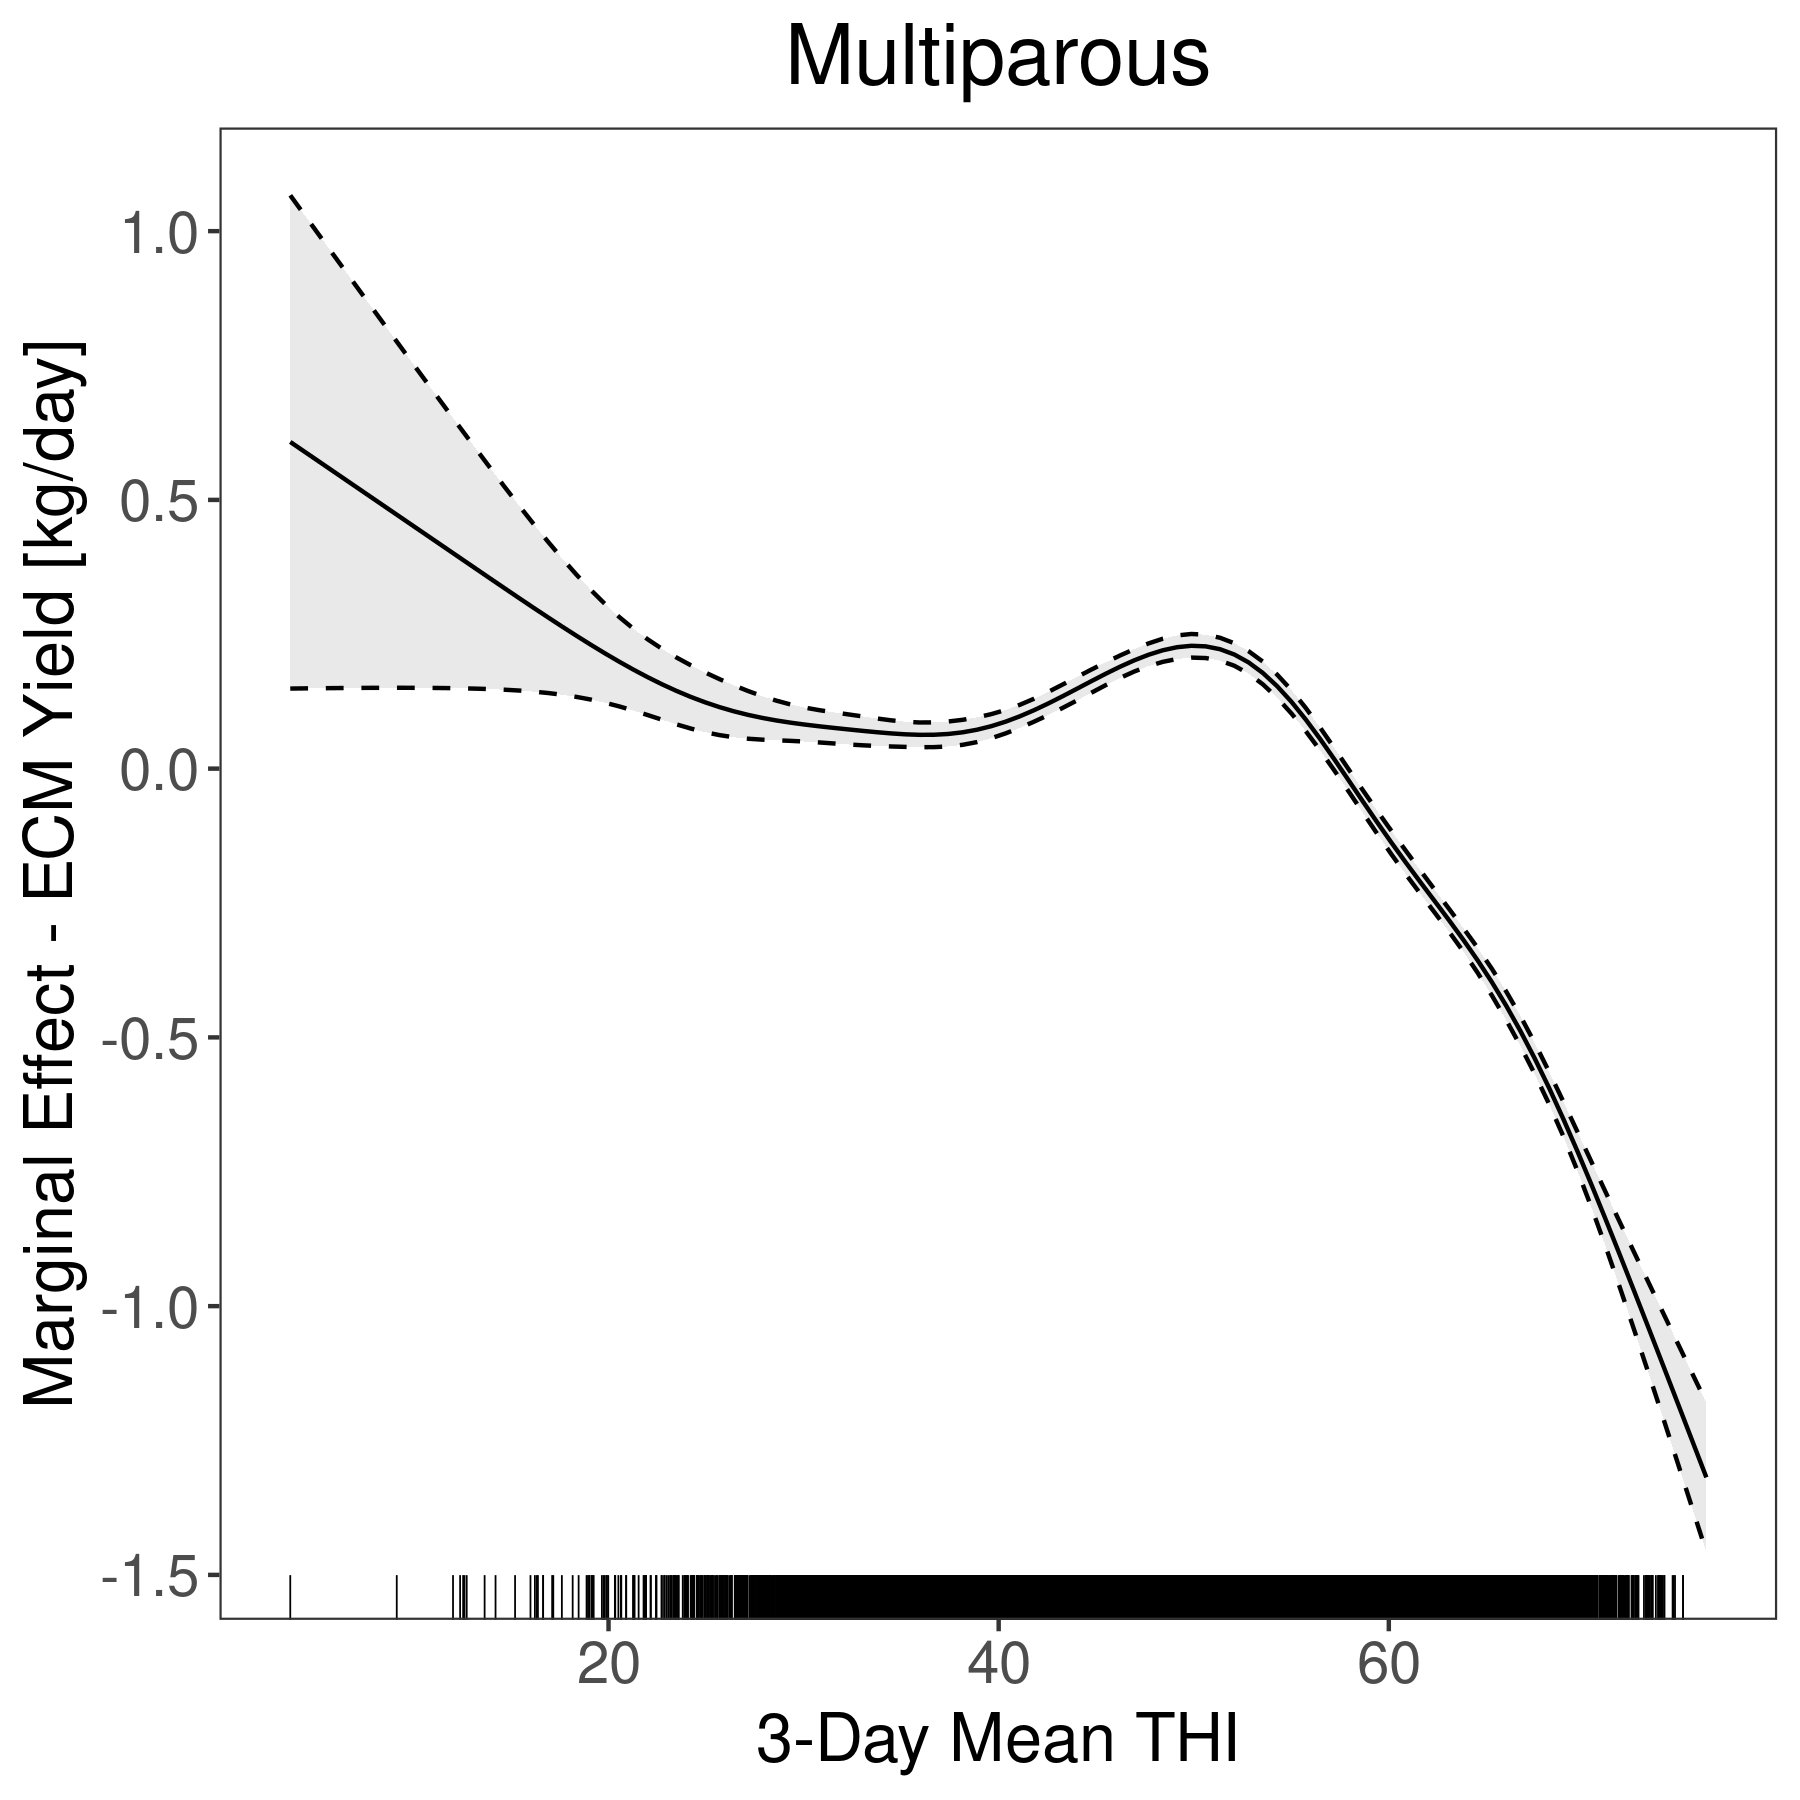
\includegraphics[width=\textwidth]{thesis/figures/models/ecm/after2010/ho_ecm_after2010/ho_ecm_after2010_marginal_thi_milk_multi.png}
    \end{subfigure}
    \hspace{0.05\textwidth} % Optional space between the figures
    \begin{subfigure}[b]{0.45\textwidth}
        \centering
        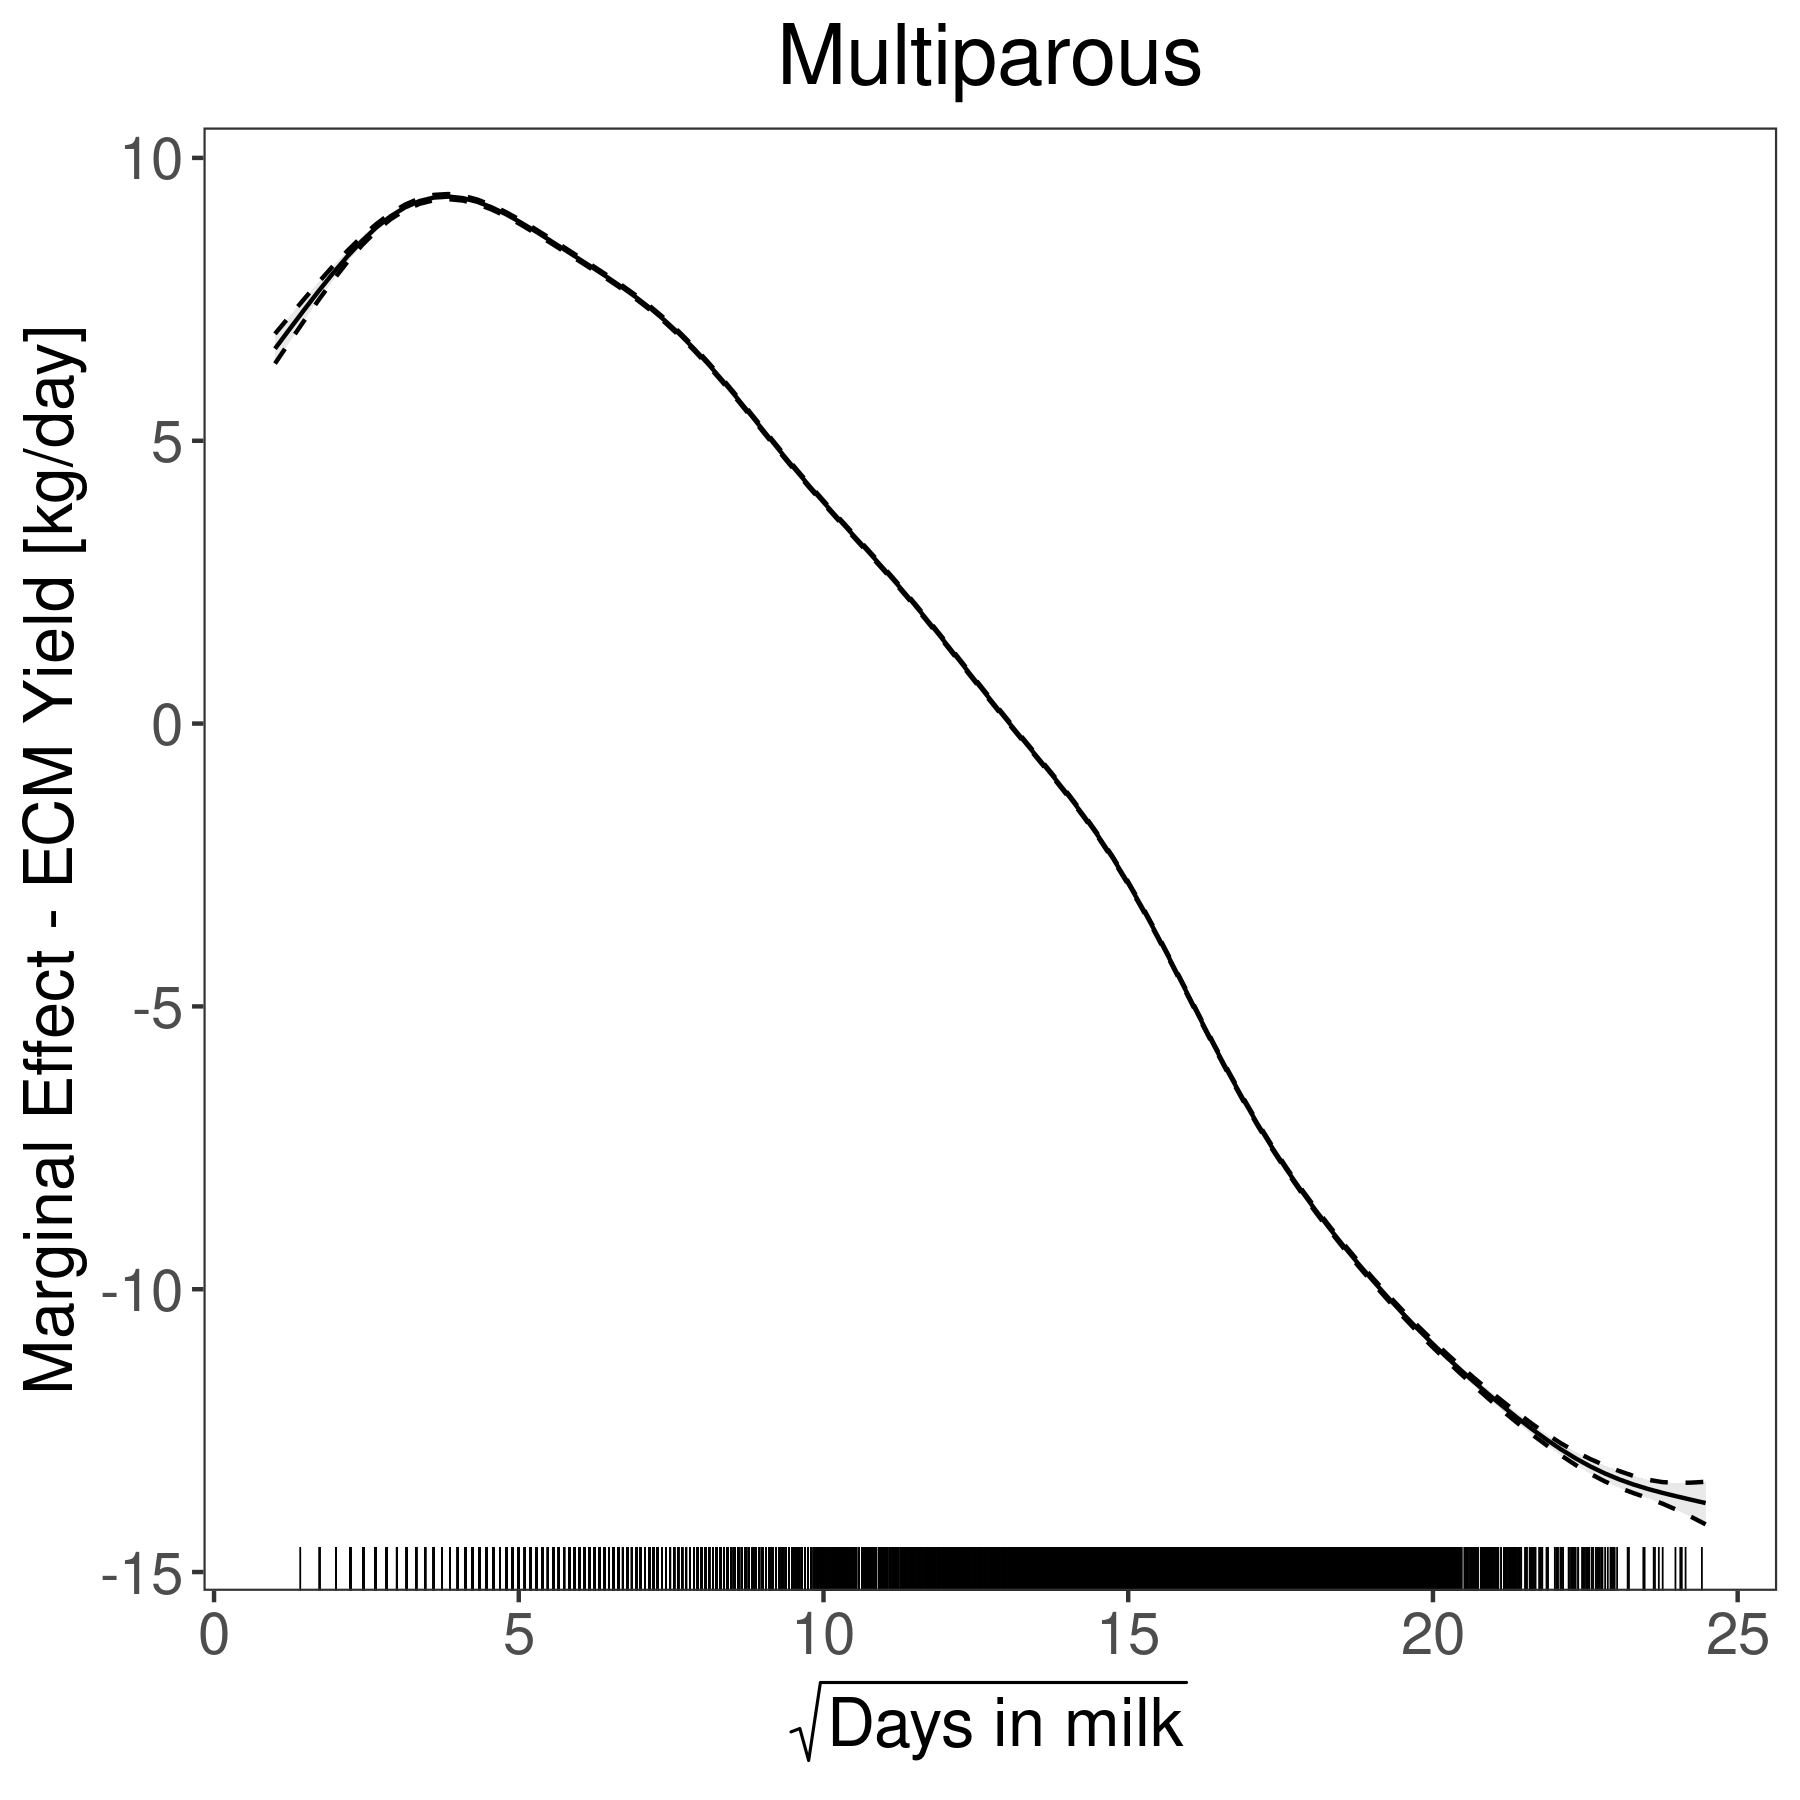
\includegraphics[width=\textwidth]{thesis/figures/models/ecm/after2010/ho_ecm_after2010/ho_ecm_after2010_marginal_dim_milk_multi.png}
    \end{subfigure}
    \caption[]{Holstein: ECM Yield - 2011 - 2023 - THI Effect and Lactation Curve}
    \label{fig:main}
\end{figure}
\addtocontents{toc}{\protect\setcounter{tocdepth}{2}}
\newpage
\section{Swiss Fleckvieh: Milk Yield}
\subsection{Full Period: 1984-2023}\label{model:sf_milk_full}
\paragraph{Model Summary} \quad \\

    \begin{table}[H]
    \centering
    \begin{tabular}{lrrrr}
    \textbf{A. parametric coefficients} & Estimate & Std. Error & t-value & p-value \\ 
       \hline
       \hline
      (Intercept) & 17.0242 & 1.8212 & 9.3480 & $<$ 0.0001 \\ 
      parityprimiparous & -2.9419 & 0.0129 & -228.3771 & $<$ 0.0001 \\ 
      year1985 & 0.3712 & 1.8309 & 0.2028 & 0.8393 \\ 
      year1986 & 0.2268 & 1.8300 & 0.1240 & 0.9013 \\ 
      year1987 & 0.1271 & 1.8312 & 0.0694 & 0.9447 \\ 
      year1988 & -0.1437 & 1.8381 & -0.0782 & 0.9377 \\ 
      year1989 & 0.6052 & 1.8388 & 0.3291 & 0.7421 \\ 
      year1990 & 0.9507 & 1.8377 & 0.5173 & 0.6049 \\ 
      year1991 & 1.1556 & 1.8380 & 0.6287 & 0.5295 \\ 
      year1992 & 1.3538 & 1.8344 & 0.7380 & 0.4605 \\ 
      year1993 & 1.3283 & 1.8344 & 0.7241 & 0.4690 \\ 
      year1994 & 1.3716 & 1.8349 & 0.7475 & 0.4548 \\ 
      year1995 & 1.5775 & 1.8387 & 0.8579 & 0.3909 \\ 
      year1996 & 1.7338 & 1.8380 & 0.9433 & 0.3455 \\ 
      year1997 & 2.1730 & 1.8387 & 1.1818 & 0.2373 \\ 
      year1998 & 3.0236 & 1.8388 & 1.6443 & 0.1001 \\ 
      year1999 & 3.1711 & 1.8415 & 1.7220 & 0.0851 \\ 
      year2000 & 3.2774 & 1.8430 & 1.7783 & 0.0754 \\ 
      year2001 & 3.5746 & 1.8569 & 1.9250 & 0.0542 \\ 
      year2002 & 3.8156 & 1.8496 & 2.0629 & 0.0391 \\ 
      year2003 & 4.3135 & 1.8487 & 2.3332 & 0.0196 \\ 
      year2004 & 4.7284 & 1.8491 & 2.5572 & 0.0106 \\ 
      year2005 & 4.9766 & 1.8513 & 2.6881 & 0.0072 \\ 
      year2006 & 4.9384 & 1.8503 & 2.6690 & 0.0076 \\ 
      year2007 & 4.6488 & 1.8505 & 2.5122 & 0.0120 \\ 
      year2008 & 4.8172 & 1.8494 & 2.6048 & 0.0092 \\ 
      year2009 & 5.0181 & 1.8479 & 2.7156 & 0.0066 \\ 
      year2010 & 5.4518 & 1.8460 & 2.9533 & 0.0031 \\ 
      year2011 & 5.4583 & 1.8432 & 2.9613 & 0.0031 \\ 
      year2012 & 5.2552 & 1.8426 & 2.8520 & 0.0043 \\ 
      year2013 & 5.1818 & 1.8422 & 2.8128 & 0.0049 \\ 
      year2014 & 5.7797 & 1.8426 & 3.1367 & 0.0017 \\ 
      year2015 & 6.1539 & 1.8427 & 3.3396 & 0.0008 \\ 
      year2016 & 6.2885 & 1.8426 & 3.4128 & 0.0006 \\ 
      year2017 & 6.5053 & 1.8430 & 3.5297 & 0.0004 \\ 
      year2018 & 7.1383 & 1.8434 & 3.8723 & 0.0001 \\ 
      year2019 & 7.1780 & 1.8443 & 3.8920 & 0.0001 \\ 
      year2020 & 7.5655 & 1.8485 & 4.0929 & $<$ 0.0001 \\ 
      year2021 & 7.6204 & 1.8511 & 4.1166 & $<$ 0.0001 \\ 
      year2022 & 7.4968 & 1.8561 & 4.0390 & 0.0001 \\ 
      year2023 & 7.9525 & 1.8595 & 4.2767 & $<$ 0.0001 \\ 
       \hline
    \textbf{B. smooth terms} & edf & Ref.df & F-value & p-value \\ 
    \hline
    \hline
      s(thi\_mean\_t0\_3d):paritymultiparous & 8.5313 & 8.5313 & 818.9814 & $<$ 0.0001 \\ 
      s(thi\_mean\_t0\_3d):parityprimiparous & 6.5854 & 6.5854 & 43.0074 & $<$ 0.0001 \\ 
      s(days\_in\_milk\_t):paritymultiparous & 14.3606 & 14.3606 & 132550.4282 & $<$ 0.0001 \\ 
      s(days\_in\_milk\_t):parityprimiparous & 13.2311 & 13.2311 & 13978.4516 & $<$ 0.0001 \\  
       \hline
    \end{tabular}
    \caption[]{Swiss Fleckvieh: Milk Yield - 1984-2023 - GAMM model summary without random effect terms.}
    \end{table}

\newpage
\begin{table}[H]
\centering
\begin{tabular}
{l | r | r | r | r}
\textbf{Smooth Term Fixed Effect} & Est. & SE & z & p\\
\hline
\hline
s(thi\_mean\_t0\_3d):multiFx1 & 0.2331 & 0.0891 & 2.62 & 0.0089\\
s(thi\_mean\_t0\_3d):primiFx1 & 0.3444 & 0.1052 & 3.27 & 0.0011\\
s(days\_in\_milk\_):multiFx1 & 1.7043 & 0.5298 & 3.22 & 0.0013\\
s(days\_in\_milk\_):primiFx1 & 0.5335 & 0.5824 & 0.92 & 0.3596\\
\hline
\textbf{Variance Component} & Estimated $\sigma$ & & & \\
\hline
\hline
$\sigma_\alpha$ & 2.6926 & & & \\
$\sigma_\iota$ & 0.8616 & & & \\
$\sigma_\phi$ & 2.8181 & & & \\
s(thi\_mean\_t0\_3d):multi &  2.2342 & & & \\
s(days\_in\_milk\_):primi & 5.7610 & & & \\
s(days\_in\_milk\_):multi & 8.3967 & & & \\
s(thi\_mean\_t0\_3d):primi & 1.1497 & & & \\
Residual & 3.1180 & & & \\
\end{tabular}
\caption[]{Swiss Fleckvieh: Milk Yield - 1984-2023 - Mixed Model Summary - Smooth Terms and Random Effects.}
\end{table}

\paragraph{Model Diagnostics} \quad \\
\begin{figure}[H]
    \centering
    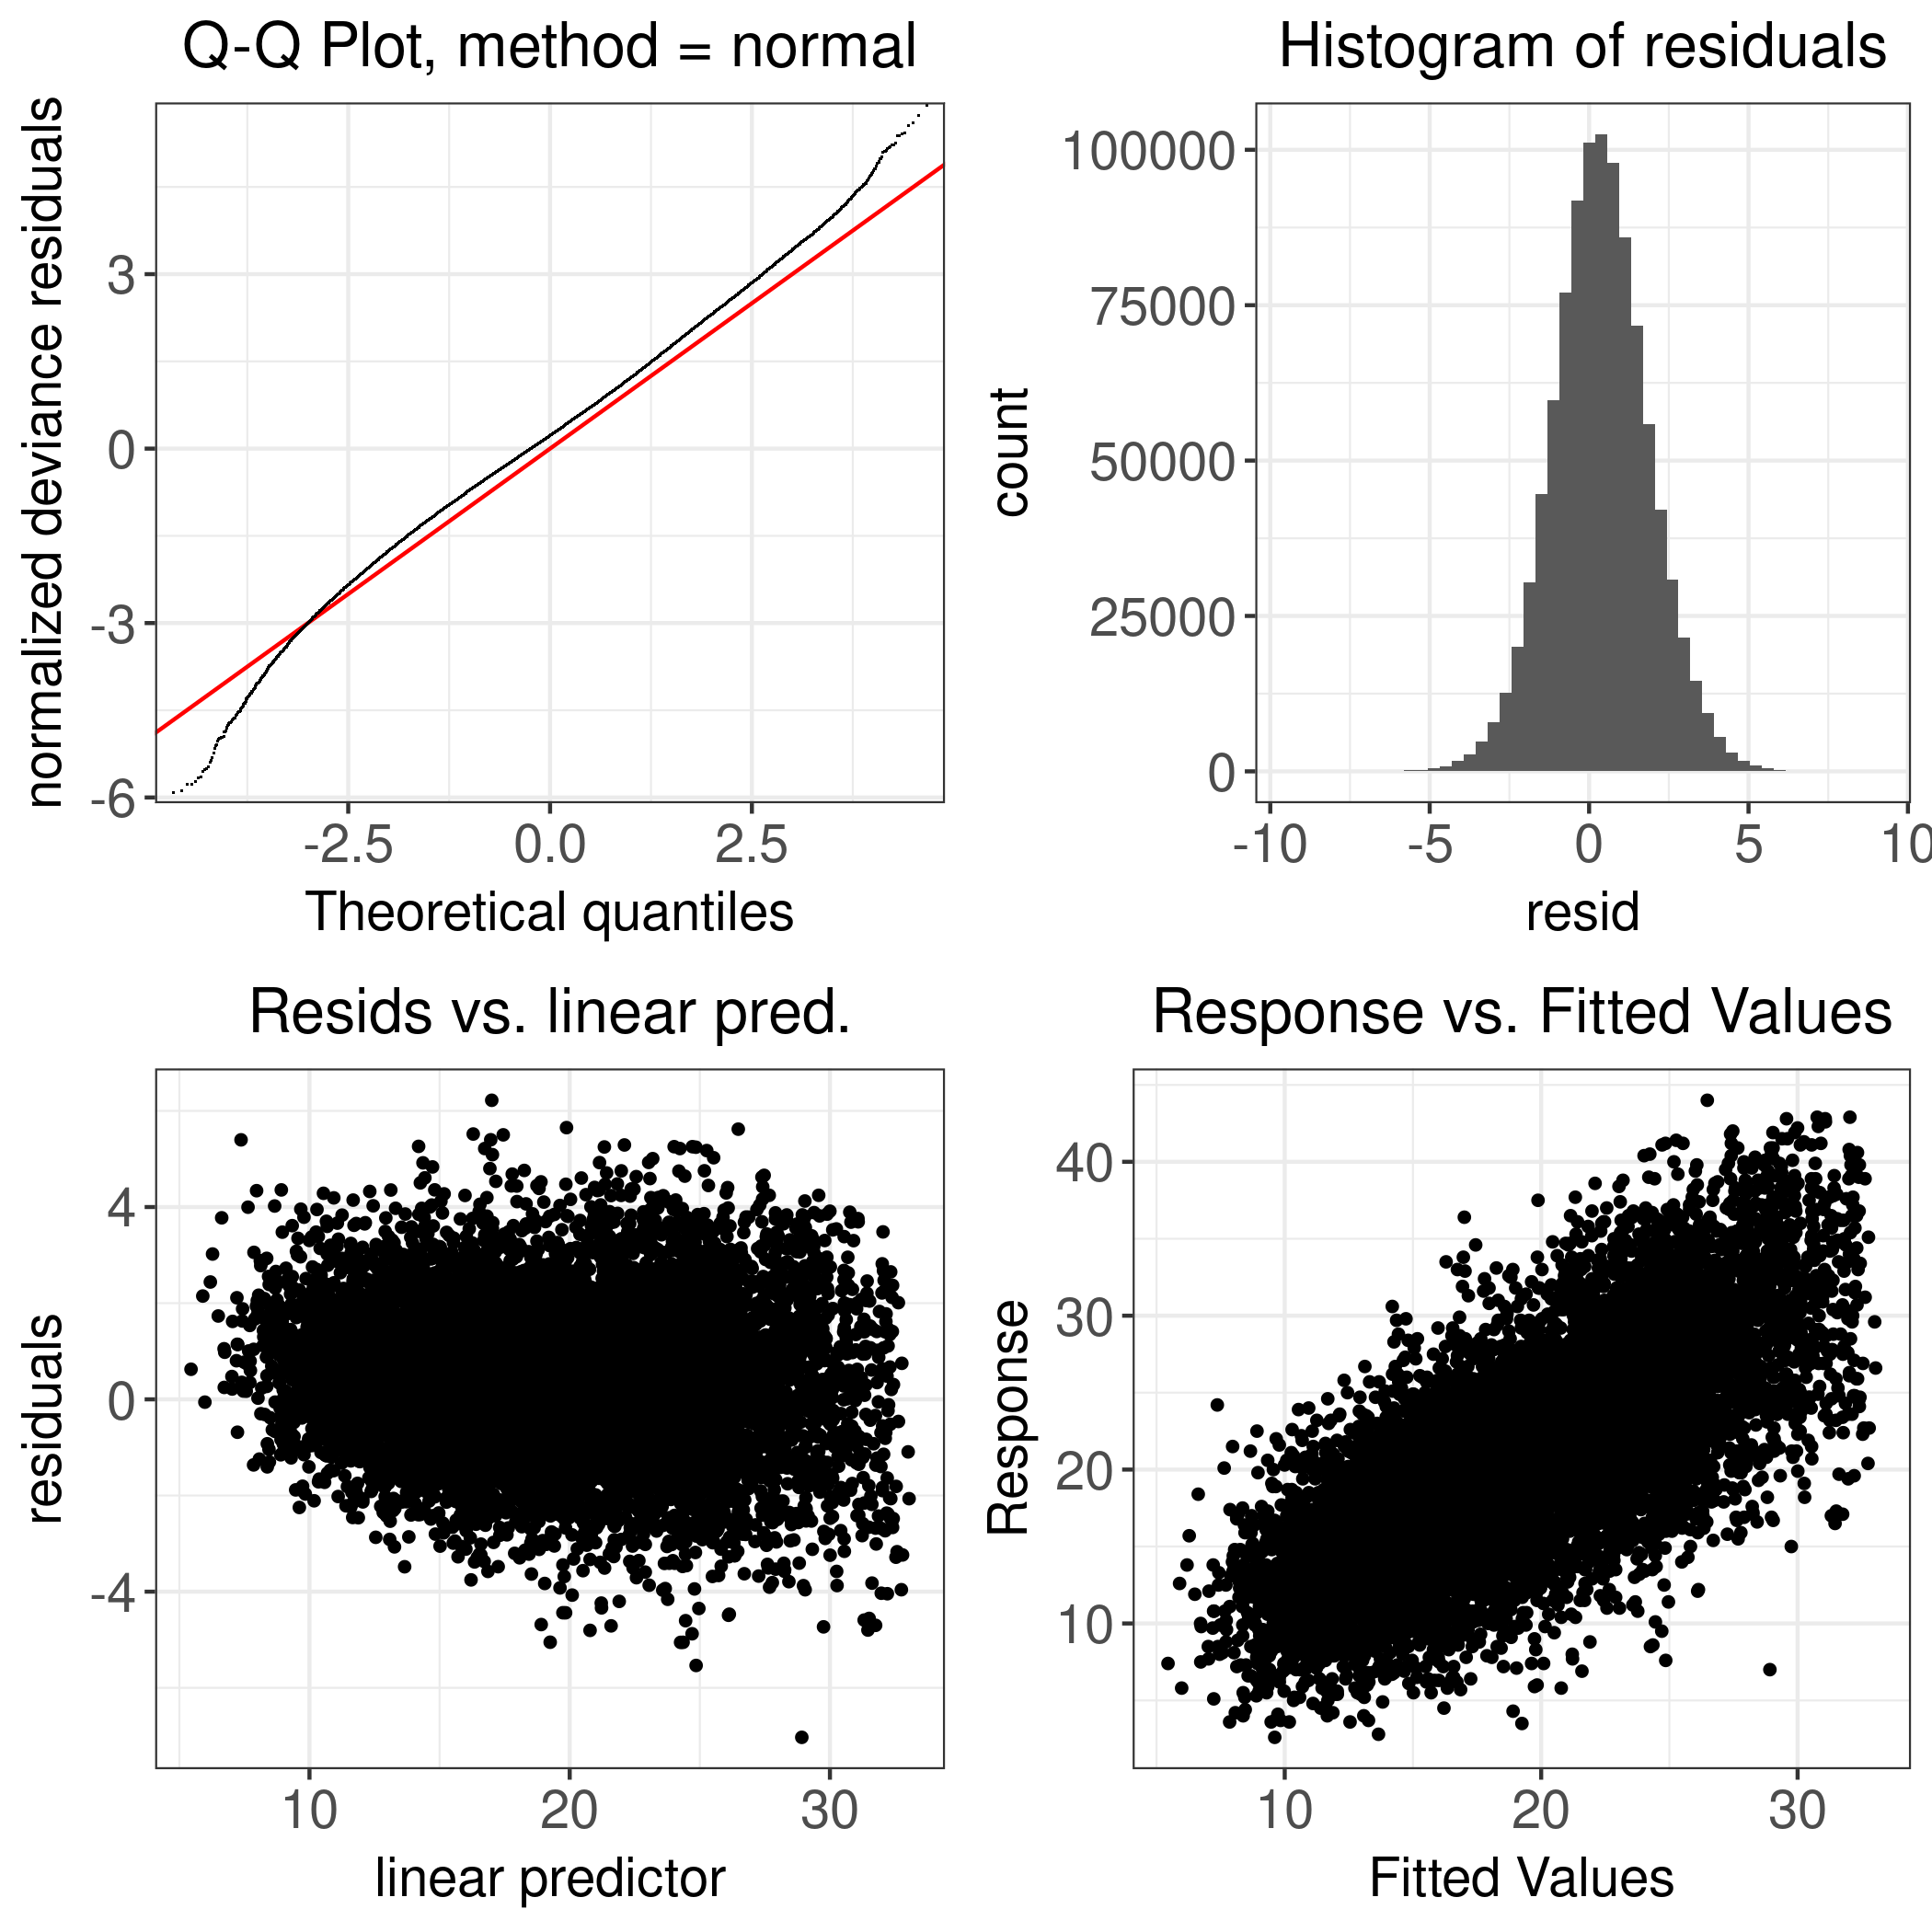
\includegraphics[width=0.6\textwidth]{thesis/figures/models/milk/full/sf_milk_full/sf_milk_full_diagnostics.png}
    \caption[]{Swiss Fleckvieh: Milk Yield - 1984-2023 - Diagnostic Plot}
\end{figure}

\newpage
\paragraph{THI Effect and Lactation Curve} \quad \\
\begin{figure}[H]
    \centering
    \begin{subfigure}[b]{0.45\textwidth}
        \centering
        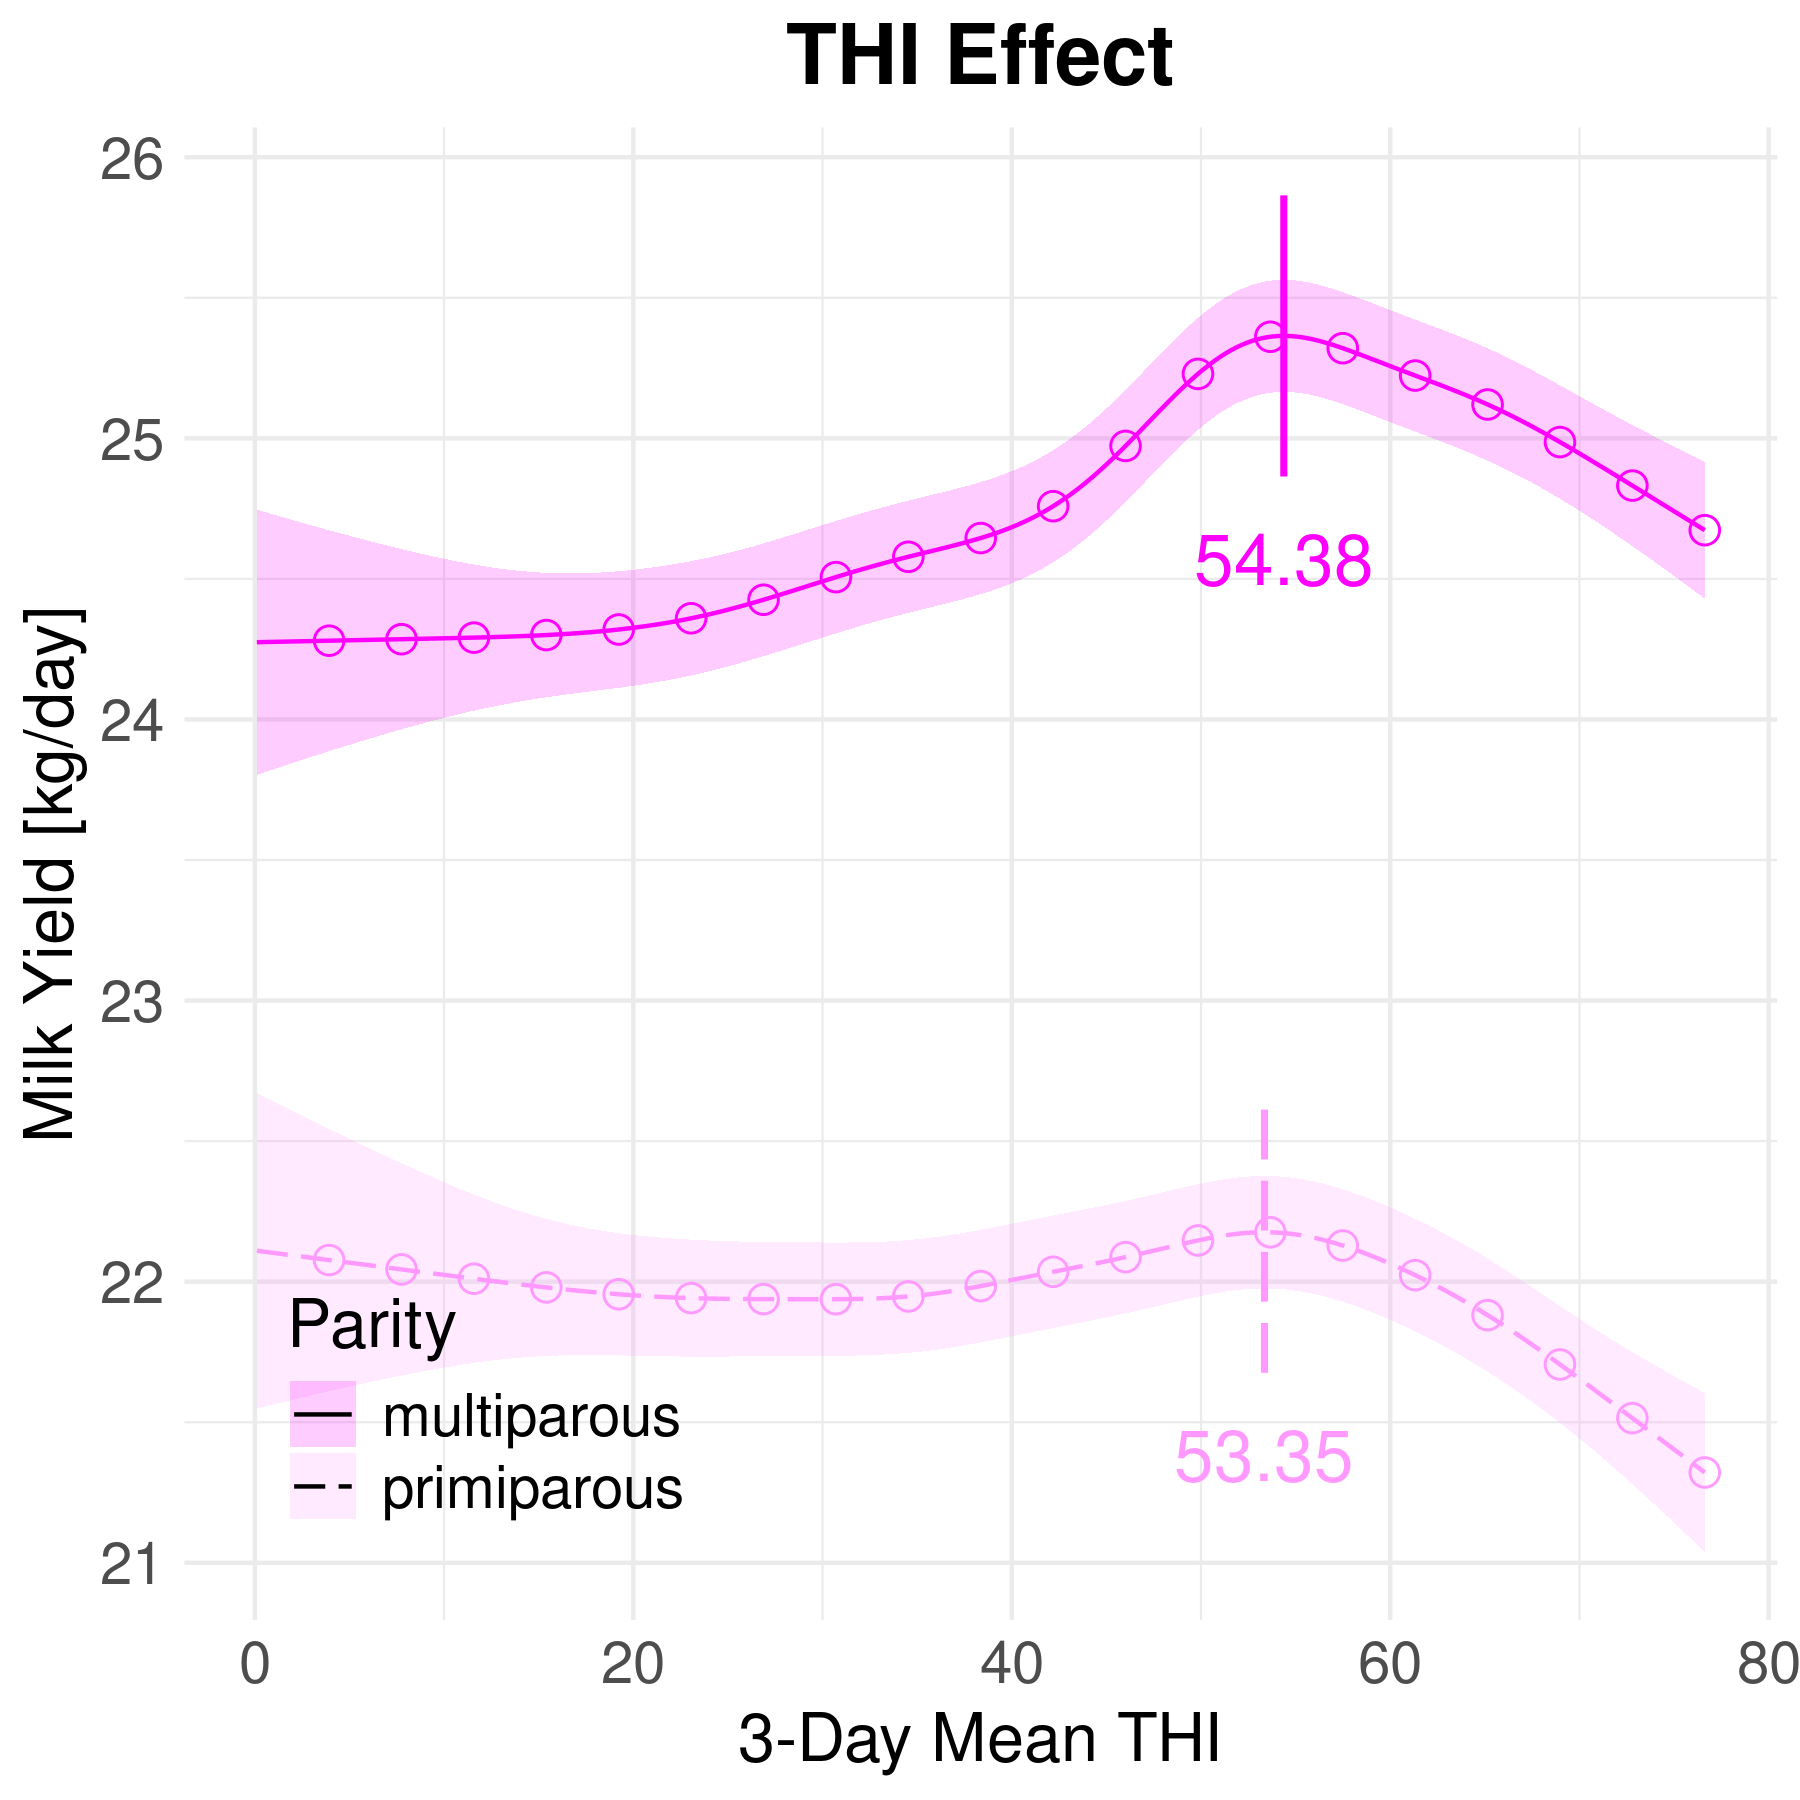
\includegraphics[width=\textwidth]{thesis/figures/models/milk/full/sf_milk_full/sf_milk_full_marginal_thi_milk_combined.png}
    \end{subfigure}
    \hspace{0.05\textwidth} % Optional space between the figures
    \begin{subfigure}[b]{0.45\textwidth}
        \centering
        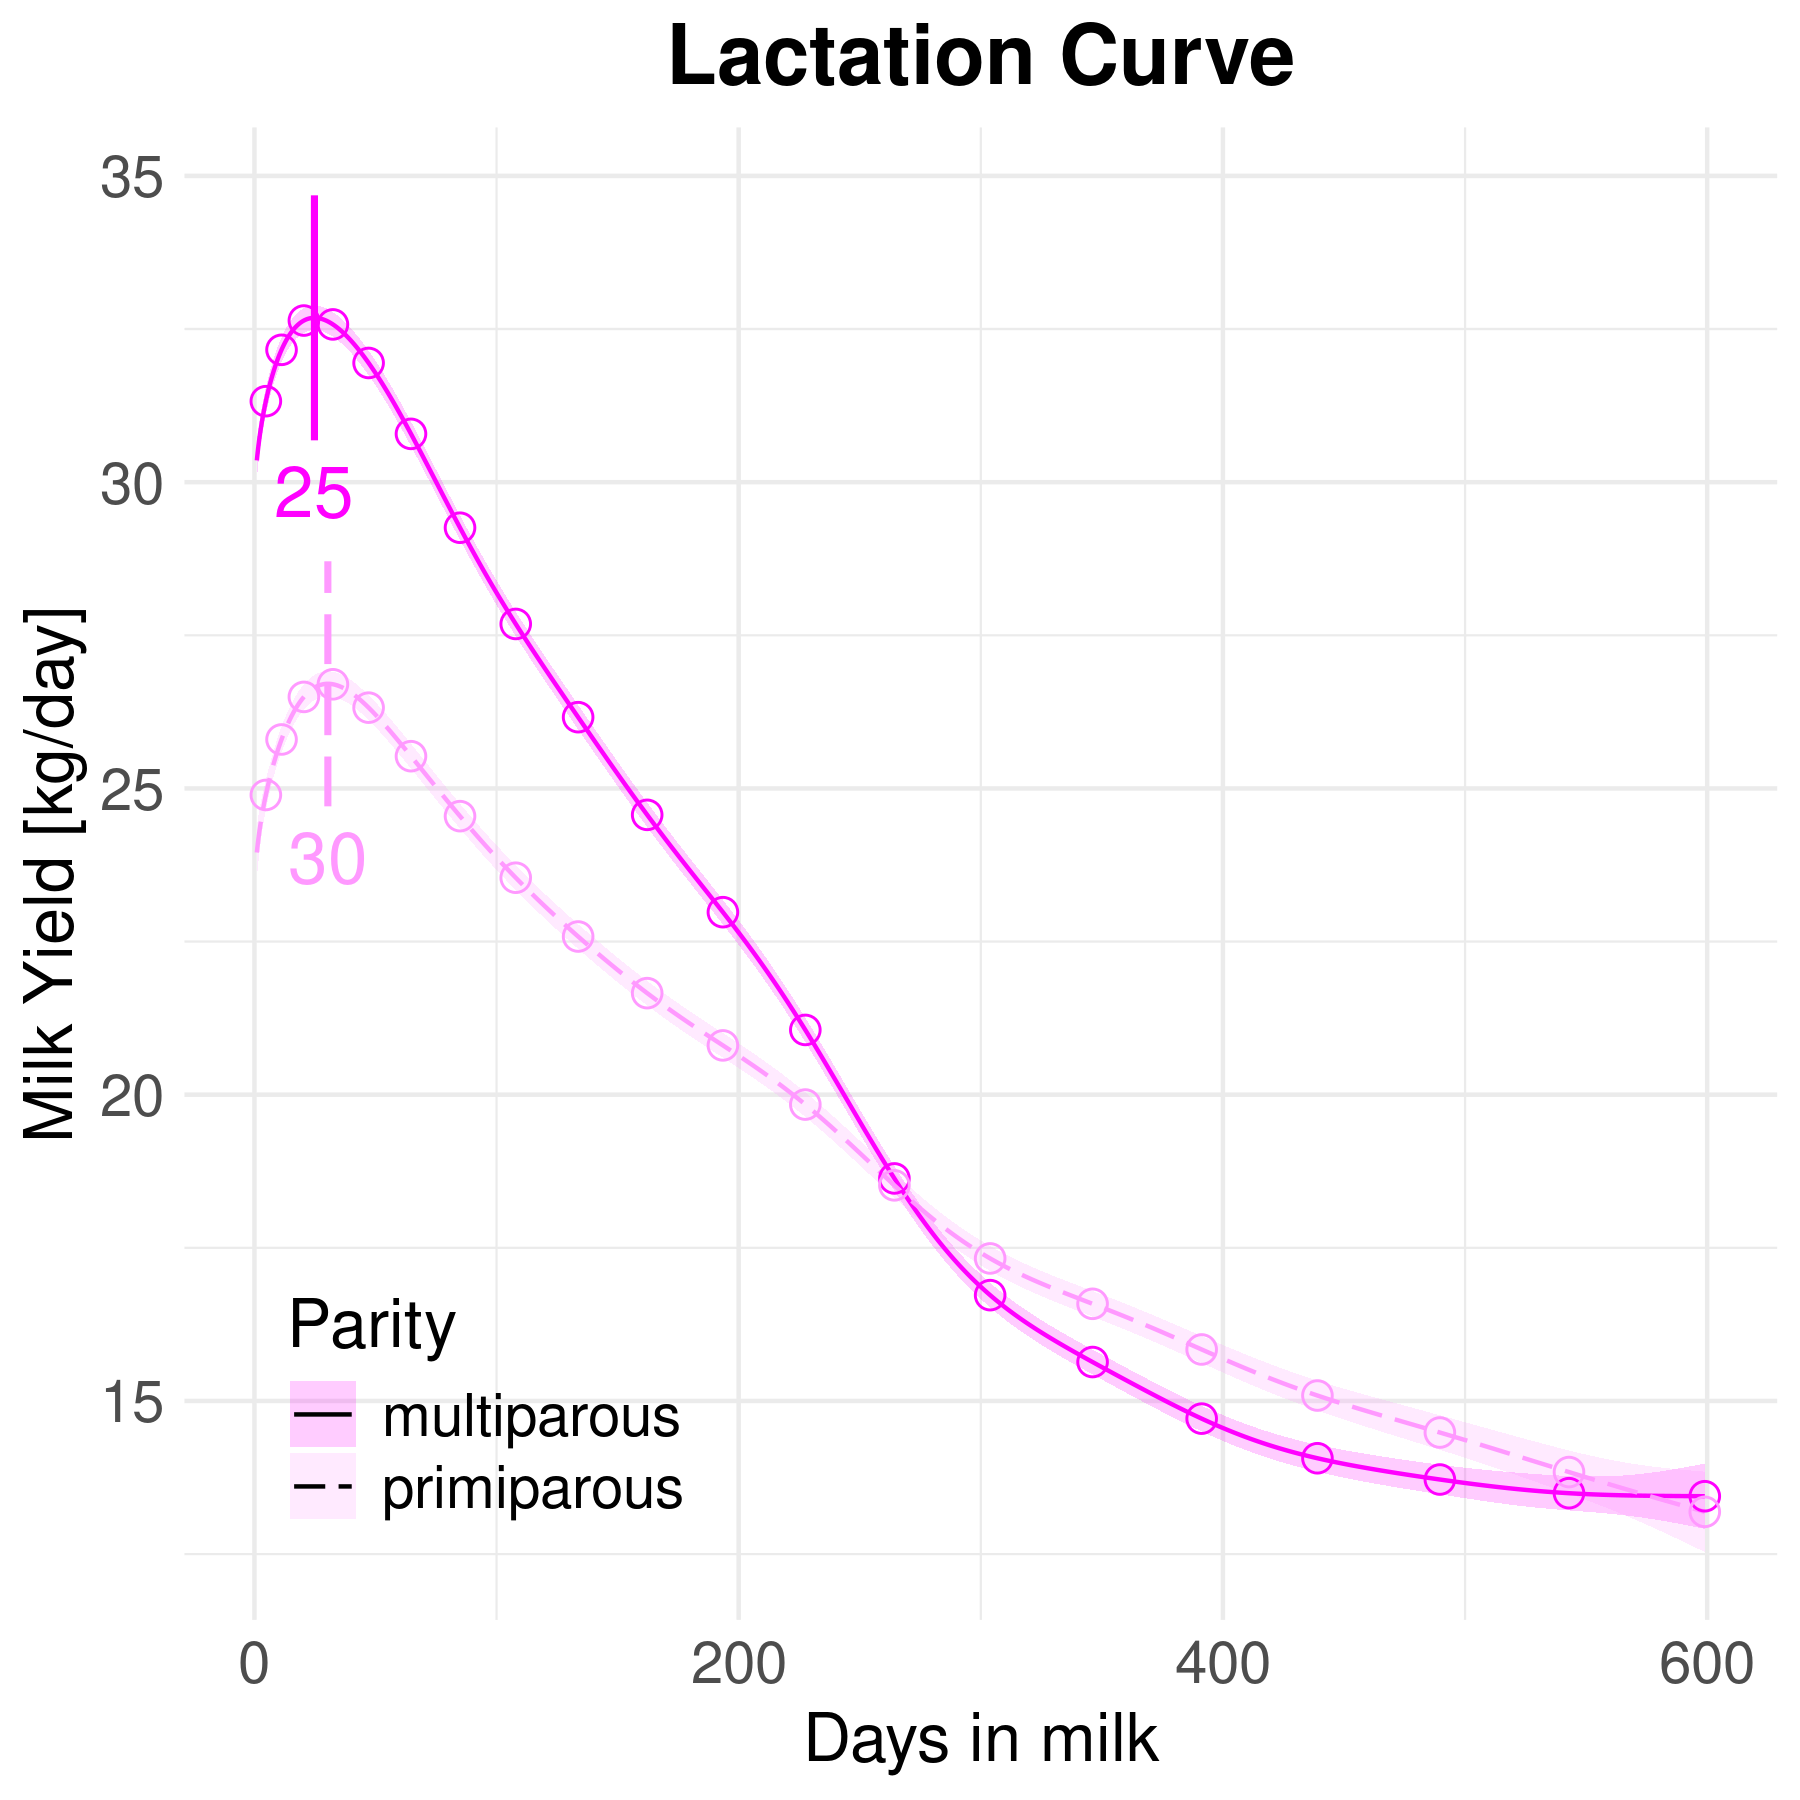
\includegraphics[width=\textwidth]{thesis/figures/models/milk/full/sf_milk_full/sf_milk_full_marginal_dim_milk_combined.png}
    \end{subfigure}
    \begin{subfigure}[b]{0.45\textwidth}
        \centering
        \includegraphics[width=\textwidth]{thesis/figures/models/milk/full/sf_milk_full/sf_milk_full_marginal_thi_milk_primi.png}
    \end{subfigure}
    \hspace{0.05\textwidth} % Optional space between the figures
    \begin{subfigure}[b]{0.45\textwidth}
        \centering
        \includegraphics[width=\textwidth]{thesis/figures/models/milk/full/sf_milk_full/sf_milk_full_marginal_dim_milk_primi.png}
    \end{subfigure}
    \begin{subfigure}[b]{0.45\textwidth}
        \centering
        \includegraphics[width=\textwidth]{thesis/figures/models/milk/full/sf_milk_full/sf_milk_full_marginal_thi_milk_multi.png}
    \end{subfigure}
    \hspace{0.05\textwidth} % Optional space between the figures
    \begin{subfigure}[b]{0.45\textwidth}
        \centering
        \includegraphics[width=\textwidth]{thesis/figures/models/milk/full/sf_milk_full/sf_milk_full_marginal_dim_milk_multi.png}
    \end{subfigure}
    \caption[]{Swiss Fleckvieh: Milk Yield - 1984 - 2023 - THI Effect and Lactation Curve}
    \label{fig:main}
\end{figure}

\subsection{Split Period: Until 2010 - After 2010}
\addtocontents{toc}{\protect\setcounter{tocdepth}{-1}}
\subsubsection{Split Period: 1984 - 2010}\label{model:sf_milk_before}
\paragraph{Model Summary} \quad \\

    \begin{table}[H]
    \centering
    \begin{tabular}{lrrrr}
    \textbf{A. parametric coefficients} & Estimate & Std. Error & t-value & p-value \\ 
       \hline
       \hline
      (Intercept) & 16.9035 & 0.3658 & 46.2066 & $<$ 0.0001 \\ 
      parityprimiparous & -2.7346 & 0.0138 & -198.6779 & $<$ 0.0001 \\ 
      year1985 & 0.4515 & 0.2804 & 1.6103 & 0.1073 \\ 
      year1986 & 0.3178 & 0.3341 & 0.9510 & 0.3416 \\ 
      year1987 & 0.2380 & 0.3534 & 0.6736 & 0.5006 \\ 
      year1988 & 0.0232 & 0.3872 & 0.0600 & 0.9522 \\ 
      year1989 & 0.7996 & 0.3910 & 2.0451 & 0.0408 \\ 
      year1990 & 1.1652 & 0.3833 & 3.0397 & 0.0024 \\ 
      year1991 & 1.4053 & 0.3711 & 3.7868 & 0.0002 \\ 
      year1992 & 1.6217 & 0.3462 & 4.6846 & $<$ 0.0001 \\ 
      year1993 & 1.6209 & 0.3497 & 4.6347 & $<$ 0.0001 \\ 
      year1994 & 1.6641 & 0.3651 & 4.5578 & $<$ 0.0001 \\ 
      year1995 & 1.9199 & 0.4094 & 4.6900 & $<$ 0.0001 \\ 
      year1996 & 2.1351 & 0.4138 & 5.1595 & $<$ 0.0001 \\ 
      year1997 & 2.5677 & 0.4256 & 6.0334 & $<$ 0.0001 \\ 
      year1998 & 3.4175 & 0.4545 & 7.5191 & $<$ 0.0001 \\ 
      year1999 & 3.5626 & 0.4510 & 7.9000 & $<$ 0.0001 \\ 
      year2000 & 3.7240 & 0.4591 & 8.1121 & $<$ 0.0001 \\ 
      year2001 & 4.0732 & 0.4673 & 8.7165 & $<$ 0.0001 \\ 
      year2002 & 4.3548 & 0.4508 & 9.6605 & $<$ 0.0001 \\ 
      year2003 & 4.8981 & 0.4394 & 11.1471 & $<$ 0.0001 \\ 
      year2004 & 5.4440 & 0.4520 & 12.0437 & $<$ 0.0001 \\ 
      year2005 & 5.7965 & 0.4626 & 12.5311 & $<$ 0.0001 \\ 
      year2006 & 5.8531 & 0.4836 & 12.1040 & $<$ 0.0001 \\ 
      year2007 & 5.6656 & 0.4880 & 11.6103 & $<$ 0.0001 \\ 
      year2008 & 5.9522 & 0.4987 & 11.9352 & $<$ 0.0001 \\ 
      year2009 & 6.4429 & 0.5211 & 12.3638 & $<$ 0.0001 \\ 
      year2010 & 7.0430 & 0.5707 & 12.3418 & $<$ 0.0001 \\ 
       \hline
    \textbf{B. smooth terms} & edf & Ref.df & F-value & p-value \\ 
    \hline
    \hline
      s(thi\_mean\_t0\_3d):paritymultiparous & 8.8565 & 8.8565 & 828.8023 & $<$ 0.0001 \\ 
      s(thi\_mean\_t0\_3d):parityprimiparous & 6.8104 & 6.8104 & 36.0865 & $<$ 0.0001 \\ 
      s(days\_in\_milk\_t):paritymultiparous & 14.2457 & 14.2457 & 139197.9545 & $<$ 0.0001 \\ 
      s(days\_in\_milk\_t):parityprimiparous & 13.2024 & 13.2024 & 14397.4338 & $<$ 0.0001 \\  
       \hline
    \end{tabular}
    \caption[]{Swiss Fleckvieh: Milk Yield - 1984-2010 - GAMM model summary without random effect terms.}
    \end{table}

\newpage
\begin{table}[H]
\centering
\begin{tabular}
{l | r | r | r | r}
\textbf{Smooth Term Fixed Effect} & Est. & SE & z & p\\
\hline
\hline
s(thi\_mean\_t0\_3d):multiFx1 & 0.2333 & 0.0852 & 2.74 & 0.0062\\
s(thi\_mean\_t0\_3d):primiFx1 & 0.2388 & 0.0987 & 2.42 & 0.0155\\
s(days\_in\_milk\_):multiFx1 & 1.3398 & 0.5299 & 2.53 & 0.0114\\
s(days\_in\_milk\_):primiFx1 & 0.3073 & 0.5533 & 0.56 & 0.5786\\
\hline
\textbf{Variance Component} & Estimated $\sigma$ & & & \\
\hline
\hline
$\sigma_\alpha$ & 2.5865 & & & \\
$\sigma_\iota$ & 0.8711 & & & \\
$\sigma_\phi$ & 2.5999 & & & \\
s(thi\_mean\_t0\_3d):multi &  3.8918 & & & \\
s(days\_in\_milk\_):primi & 5.4281 & & & \\
s(days\_in\_milk\_):multi & 7.5874 & & & \\
s(thi\_mean\_t0\_3d):primi & 1.1463 & & & \\
Residual & 2.9720 & & & \\
\end{tabular}
\caption[]{Swiss Fleckvieh: Milk Yield - 1984-2010 - Mixed Model Summary - Smooth Terms and Random Effects.}
\end{table}


\paragraph{Model Diagnostics} \quad \\
\begin{figure}[H]
    \centering
    \includegraphics[width=0.6\textwidth]{thesis/figures/models/milk/before2010/sf_milk_before2010/sf_milk_before2010_diagnostics.png}
    \caption[]{Swiss Fleckvieh: Milk Yield - 1984-2010 - Diagnostic Plot}
\end{figure}

\newpage
\paragraph{THI Effect and Lactation Curve} \quad \\
\begin{figure}[H]
    \centering
    \begin{subfigure}[b]{0.45\textwidth}
        \centering
        \includegraphics[width=\textwidth]{thesis/figures/models/milk/before2010/sf_milk_before2010/sf_milk_before2010_marginal_thi_milk_combined.png}
    \end{subfigure}
    \hspace{0.05\textwidth} % Optional space between the figures
    \begin{subfigure}[b]{0.45\textwidth}
        \centering
        \includegraphics[width=\textwidth]{thesis/figures/models/milk/before2010/sf_milk_before2010/sf_milk_before2010_marginal_dim_milk_combined.png}
    \end{subfigure}
    \begin{subfigure}[b]{0.45\textwidth}
        \centering
        \includegraphics[width=\textwidth]{thesis/figures/models/milk/before2010/sf_milk_before2010/sf_milk_before2010_marginal_thi_milk_primi.png}
    \end{subfigure}
    \hspace{0.05\textwidth} % Optional space between the figures
    \begin{subfigure}[b]{0.45\textwidth}
        \centering
        \includegraphics[width=\textwidth]{thesis/figures/models/milk/before2010/sf_milk_before2010/sf_milk_before2010_marginal_dim_milk_primi.png}
    \end{subfigure}
    \begin{subfigure}[b]{0.45\textwidth}
        \centering
        \includegraphics[width=\textwidth]{thesis/figures/models/milk/before2010/sf_milk_before2010/sf_milk_before2010_marginal_thi_milk_multi.png}
    \end{subfigure}
    \hspace{0.05\textwidth} % Optional space between the figures
    \begin{subfigure}[b]{0.45\textwidth}
        \centering
        \includegraphics[width=\textwidth]{thesis/figures/models/milk/before2010/sf_milk_before2010/sf_milk_before2010_marginal_dim_milk_multi.png}
    \end{subfigure}
    \caption[]{Swiss Fleckvieh: Milk Yield - 1984 - 2010 - THI Effect and Lactation Curve}
    \label{fig:main}
\end{figure}

\subsubsection{Split Period: 2010 - 2023}\label{model:sf_milk_after}

\paragraph{Model Summary} \quad \\

    \begin{table}[H]
    \centering
    \begin{tabular}{lrrrr}
    \textbf{A. parametric coefficients} & Estimate & Std. Error & t-value & p-value \\ 
       \hline
       \hline
      (Intercept) & 21.7530 & 0.2595 & 83.8176 & $<$ 0.0001 \\ 
      parityprimiparous & -3.3595 & 0.0149 & -224.7296 & $<$ 0.0001 \\ 
      year2012 & -0.1631 & 0.3056 & -0.5337 & 0.5936 \\ 
      year2013 & -0.3339 & 0.2926 & -1.1414 & 0.2537 \\ 
      year2014 & 0.2384 & 0.2906 & 0.8203 & 0.4121 \\ 
      year2015 & 0.4961 & 0.2957 & 1.6777 & 0.0934 \\ 
      year2016 & 0.8626 & 0.2984 & 2.8910 & 0.0038 \\ 
      year2017 & 1.2313 & 0.2939 & 4.1894 & $<$ 0.0001 \\ 
      year2018 & 1.6165 & 0.2967 & 5.4488 & $<$ 0.0001 \\ 
      year2019 & 1.7695 & 0.2943 & 6.0121 & $<$ 0.0001 \\ 
      year2020 & 2.0975 & 0.3029 & 6.9248 & $<$ 0.0001 \\ 
      year2021 & 2.3398 & 0.2847 & 8.2183 & $<$ 0.0001 \\ 
      year2022 & 2.1729 & 0.3008 & 7.2243 & $<$ 0.0001 \\ 
      year2023 & 2.3855 & 0.2954 & 8.0764 & $<$ 0.0001 \\ 
       \hline
    \textbf{B. smooth terms} & edf & Ref.df & F-value & p-value \\ 
    \hline
    \hline
      s(thi\_mean\_t0\_3d):paritymultiparous & 8.1653 & 8.1653 & 699.8806 & $<$ 0.0001 \\ 
      s(thi\_mean\_t0\_3d):parityprimiparous & 6.5967 & 6.5967 & 37.1793 & $<$ 0.0001 \\ 
      s(days\_in\_milk\_t):paritymultiparous & 14.5202 & 14.5202 & 113726.1561 & $<$ 0.0001 \\ 
      s(days\_in\_milk\_t):parityprimiparous & 13.5621 & 13.5621 & 11375.9787 & $<$ 0.0001 \\  
       \hline
    \end{tabular}
    \caption[]{Swiss Fleckvieh: Milk Yield - 2011-2023 - GAMM model summary without random effect terms.}
    \end{table}

\newpage
\begin{table}[H]
\centering
\begin{tabular}
{l | r | r | r | r}
\textbf{Smooth Term Fixed Effect} & Est. & SE & z & p\\
\hline
\hline
s(thi\_mean\_t0\_3d):multiFx1 & 0.1716 & 0.0901 & 1.91 & 0.0568\\
s(thi\_mean\_t0\_3d):primiFx1 & -0.2638 & 0.1058 & -2.49 & 0.0126\\
s(days\_in\_milk\_):multiFx1 & 3.0173 & 0.4977 & 6.06 & $<$ 1e-08\\
s(days\_in\_milk\_):primiFx1 & 3.2102 & 0.6274 & 5.12 & $<$ 1e-06\\
\hline
\textbf{Variance Component} & Estimated $\sigma$ & & & \\
\hline
\hline
$\sigma_\alpha$ & 2.7938 & & & \\
$\sigma_\iota$ & 1.0653 & & & \\
$\sigma_\phi$ & 3.2540 & & & \\
s(thi\_mean\_t0\_3d):multi &  1.8095 & & & \\
s(days\_in\_milk\_):primi & 7.0409 & & & \\
s(days\_in\_milk\_):multi & 9.4413 & & & \\
s(thi\_mean\_t0\_3d):primi & 1.2895 & & & \\
Residual & 3.4929 & & & \\
\end{tabular}
\caption[]{Swiss Fleckvieh: Milk Yield - 2011-2023 - Mixed Model Summary - Smooth Terms and Random Effects.}
\end{table}



\paragraph{Model Diagnostics} \quad \\
\begin{figure}[H]
    \centering
    \includegraphics[width=0.6\textwidth]{thesis/figures/models/milk/after2010/sf_milk_after2010/sf_milk_after2010_diagnostics.png}
    \caption[]{Swiss Fleckvieh: Milk Yield - 2011-2023 - Diagnostic Plot}
\end{figure}

\newpage
\paragraph{THI Effect and Lactation Curve} \quad \\
\begin{figure}[H]
    \centering
    \begin{subfigure}[b]{0.45\textwidth}
        \centering
        \includegraphics[width=\textwidth]{thesis/figures/models/milk/after2010/sf_milk_after2010/sf_milk_after2010_marginal_thi_milk_combined.png}
    \end{subfigure}
    \hspace{0.05\textwidth} % Optional space between the figures
    \begin{subfigure}[b]{0.45\textwidth}
        \centering
        \includegraphics[width=\textwidth]{thesis/figures/models/milk/after2010/sf_milk_after2010/sf_milk_after2010_marginal_dim_milk_combined.png}
    \end{subfigure}
    \begin{subfigure}[b]{0.45\textwidth}
        \centering
        \includegraphics[width=\textwidth]{thesis/figures/models/milk/after2010/sf_milk_after2010/sf_milk_after2010_marginal_thi_milk_primi.png}
    \end{subfigure}
    \hspace{0.05\textwidth} % Optional space between the figures
    \begin{subfigure}[b]{0.45\textwidth}
        \centering
        \includegraphics[width=\textwidth]{thesis/figures/models/milk/after2010/sf_milk_after2010/sf_milk_after2010_marginal_dim_milk_primi.png}
    \end{subfigure}
    \begin{subfigure}[b]{0.45\textwidth}
        \centering
        \includegraphics[width=\textwidth]{thesis/figures/models/milk/after2010/sf_milk_after2010/sf_milk_after2010_marginal_thi_milk_multi.png}
    \end{subfigure}
    \hspace{0.05\textwidth} % Optional space between the figures
    \begin{subfigure}[b]{0.45\textwidth}
        \centering
        \includegraphics[width=\textwidth]{thesis/figures/models/milk/after2010/sf_milk_after2010/sf_milk_after2010_marginal_dim_milk_multi.png}
    \end{subfigure}
    \caption[]{Swiss Fleckvieh: Milk Yield - 2011 - 2023 - THI Effect and Lactation Curve}
    \label{fig:main}
\end{figure}
\addtocontents{toc}{\protect\setcounter{tocdepth}{2}}

\section{Swiss Fleckvieh: ECM Yield}
\subsection{Full Period: 1984-2023}\label{model:sf_ecm_full}
\paragraph{Model Summary} \quad \\

    \begin{table}[H]
    \centering
    \begin{tabular}{lrrrr}
    \textbf{A. parametric coefficients} & Estimate & Std. Error & t-value & p-value \\ 
       \hline
       \hline
      (Intercept) & 18.9428 & 2.0368 & 9.3002 & $<$ 0.0001 \\ 
      parityprimiparous & -3.3689 & 0.0142 & -236.8632 & $<$ 0.0001 \\ 
      year1985 & 0.4371 & 2.0474 & 0.2135 & 0.8309 \\ 
      year1986 & 0.3102 & 2.0464 & 0.1516 & 0.8795 \\ 
      year1987 & 0.0716 & 2.0478 & 0.0349 & 0.9721 \\ 
      year1988 & -0.3584 & 2.0554 & -0.1744 & 0.8616 \\ 
      year1989 & 0.4960 & 2.0565 & 0.2412 & 0.8094 \\ 
      year1990 & 0.9176 & 2.0553 & 0.4464 & 0.6553 \\ 
      year1991 & 1.1455 & 2.0556 & 0.5572 & 0.5774 \\ 
      year1992 & 1.4593 & 2.0517 & 0.7113 & 0.4769 \\ 
      year1993 & 1.3829 & 2.0517 & 0.6740 & 0.5003 \\ 
      year1994 & 1.2177 & 2.0522 & 0.5933 & 0.5530 \\ 
      year1995 & 1.5433 & 2.0564 & 0.7505 & 0.4530 \\ 
      year1996 & 1.7761 & 2.0557 & 0.8640 & 0.3876 \\ 
      year1997 & 2.2786 & 2.0564 & 1.1081 & 0.2678 \\ 
      year1998 & 3.1880 & 2.0566 & 1.5502 & 0.1211 \\ 
      year1999 & 3.1331 & 2.0596 & 1.5212 & 0.1282 \\ 
      year2000 & 3.0081 & 2.0612 & 1.4594 & 0.1445 \\ 
      year2001 & 3.3840 & 2.0762 & 1.6299 & 0.1031 \\ 
      year2002 & 3.4445 & 2.0684 & 1.6653 & 0.0959 \\ 
      year2003 & 3.9752 & 2.0675 & 1.9227 & 0.0545 \\ 
      year2004 & 4.4635 & 2.0679 & 2.1585 & 0.0309 \\ 
      year2005 & 4.8537 & 2.0704 & 2.3444 & 0.0191 \\ 
      year2006 & 4.7686 & 2.0692 & 2.3046 & 0.0212 \\ 
      year2007 & 4.4191 & 2.0694 & 2.1354 & 0.0327 \\ 
      year2008 & 4.6589 & 2.0682 & 2.2526 & 0.0243 \\ 
      year2009 & 4.8424 & 2.0665 & 2.3433 & 0.0191 \\ 
      year2010 & 5.3358 & 2.0644 & 2.5847 & 0.0097 \\ 
      year2011 & 5.2852 & 2.0614 & 2.5639 & 0.0104 \\ 
      year2012 & 5.2468 & 2.0608 & 2.5460 & 0.0109 \\ 
      year2013 & 5.0911 & 2.0603 & 2.4711 & 0.0135 \\ 
      year2014 & 5.6526 & 2.0607 & 2.7430 & 0.0061 \\ 
      year2015 & 6.1039 & 2.0609 & 2.9618 & 0.0031 \\ 
      year2016 & 6.3861 & 2.0608 & 3.0989 & 0.0019 \\ 
      year2017 & 6.4411 & 2.0613 & 3.1249 & 0.0018 \\ 
      year2018 & 7.2593 & 2.0617 & 3.5210 & 0.0004 \\ 
      year2019 & 7.3393 & 2.0627 & 3.5581 & 0.0004 \\ 
      year2020 & 7.8516 & 2.0673 & 3.7979 & 0.0001 \\ 
      year2021 & 8.0252 & 2.0703 & 3.8763 & 0.0001 \\ 
      year2022 & 7.7722 & 2.0760 & 3.7437 & 0.0002 \\ 
      year2023 & 8.3910 & 2.0798 & 4.0346 & 0.0001 \\ 
       \hline
    \textbf{B. smooth terms} & edf & Ref.df & F-value & p-value \\ 
    \hline
    \hline
      s(thi\_mean\_t0\_3d):paritymultiparous & 8.5041 & 8.5041 & 234.1182 & $<$ 0.0001 \\ 
      s(thi\_mean\_t0\_3d):parityprimiparous & 6.4177 & 6.4177 & 140.2851 & $<$ 0.0001 \\ 
      s(days\_in\_milk\_t):paritymultiparous & 14.1442 & 14.1442 & 103387.1413 & $<$ 0.0001 \\ 
      s(days\_in\_milk\_t):parityprimiparous & 12.3534 & 12.3534 & 9446.9365 & $<$ 0.0001 \\ 
       \hline
    \end{tabular}
    \caption[]{Swiss Fleckvieh: ECM Yield - 1984-2023 - GAMM model summary without random effect terms.}
    \end{table}

\newpage
\begin{table}[H]
\centering
\begin{tabular}
{l | r | r | r | r}
\textbf{Smooth Term Fixed Effect} & Est. & SE & z & p\\
\hline
\hline
s(thi\_mean\_t0\_3d):multiFx1 & 0.4379 & 0.0980 & 4.47 & $<$ 1e-05\\
s(thi\_mean\_t0\_3d):primiFx1 & 0.5091 & 0.1123 & 4.53 & $<$ 1e-05\\
s(days\_in\_milk\_):multiFx1 & 0.1549 & 0.5426 & 0.29 & 0.7752\\
s(days\_in\_milk\_):primiFx1 & -0.4183 & 0.5123 & -0.82 & 0.4142\\
\hline
\textbf{Variance Component} & Estimated $\sigma$ & & & \\
\hline
\hline
$\sigma_\alpha$ & 2.7441 & & & \\
$\sigma_\iota$ & 0.9269 & & & \\
$\sigma_\phi$ & 3.2102 & & & \\
s(thi\_mean\_t0\_3d):multi &  2.3885 & & & \\
s(days\_in\_milk\_):primi & 4.1628 & & & \\
s(days\_in\_milk\_):multi & 7.4804 & & & \\
s(thi\_mean\_t0\_3d):primi & 1.1828 & & & \\
Residual & 3.4443 & & & \\
\end{tabular}
\caption[]{Swiss Fleckvieh: ECM Yield - 1984-2023 - Mixed Model Summary - Smooth Terms and Random Effects.}
\end{table}


\paragraph{Model Diagnostics} \quad \\
\begin{figure}[H]
    \centering
    \includegraphics[width=0.6\textwidth]{thesis/figures/models/ecm/full/sf_ecm_full/sf_ecm_full_diagnostics.png}
    \caption[]{Swiss Fleckvieh: ECM Yield - 1984-2023 - Diagnostic Plot}
\end{figure}

\newpage
\paragraph{THI Effect and Lactation Curve} \quad \\
\begin{figure}[H]
    \centering
    \begin{subfigure}[b]{0.45\textwidth}
        \centering
        \includegraphics[width=\textwidth]{thesis/figures/models/ecm/full/sf_ecm_full/sf_ecm_full_marginal_thi_milk_combined.png}
    \end{subfigure}
    \hspace{0.05\textwidth} % Optional space between the figures
    \begin{subfigure}[b]{0.45\textwidth}
        \centering
        \includegraphics[width=\textwidth]{thesis/figures/models/ecm/full/sf_ecm_full/sf_ecm_full_marginal_dim_milk_combined.png}
    \end{subfigure}
    \begin{subfigure}[b]{0.45\textwidth}
        \centering
        \includegraphics[width=\textwidth]{thesis/figures/models/ecm/full/sf_ecm_full/sf_ecm_full_marginal_thi_milk_primi.png}
    \end{subfigure}
    \hspace{0.05\textwidth} % Optional space between the figures
    \begin{subfigure}[b]{0.45\textwidth}
        \centering
        \includegraphics[width=\textwidth]{thesis/figures/models/ecm/full/sf_ecm_full/sf_ecm_full_marginal_dim_milk_primi.png}
    \end{subfigure}
    \begin{subfigure}[b]{0.45\textwidth}
        \centering
        \includegraphics[width=\textwidth]{thesis/figures/models/ecm/full/sf_ecm_full/sf_ecm_full_marginal_thi_milk_multi.png}
    \end{subfigure}
    \hspace{0.05\textwidth} % Optional space between the figures
    \begin{subfigure}[b]{0.45\textwidth}
        \centering
        \includegraphics[width=\textwidth]{thesis/figures/models/ecm/full/sf_ecm_full/sf_ecm_full_marginal_dim_milk_multi.png}
    \end{subfigure}
    \caption[]{Swiss Fleckvieh: ECM Yield - 1984 - 2023 - THI Effect and Lactation Curve}
    \label{fig:main}
\end{figure}

\subsection{Split Period: Until 2010 - After 2010}
\addtocontents{toc}{\protect\setcounter{tocdepth}{-1}}
\subsubsection{Split Period: 1984 - 2010}\label{model:sf_ecm_before}

\paragraph{Model Summary} \quad \\

    \begin{table}[H]
    \centering
    \begin{tabular}{lrrrr}
    \textbf{A. parametric coefficients} & Estimate & Std. Error & t-value & p-value \\ 
       \hline
       \hline
      (Intercept) & 18.6574 & 0.3504 & 53.2489 & $<$ 0.0001 \\ 
      parityprimiparous & -3.1387 & 0.0130 & -242.3247 & $<$ 0.0001 \\ 
      year1985 & 0.5924 & 0.1977 & 2.9963 & 0.0027 \\ 
      year1986 & 0.5314 & 0.2944 & 1.8051 & 0.0711 \\ 
      year1987 & 0.2646 & 0.3287 & 0.8049 & 0.4209 \\ 
      year1988 & -0.0889 & 0.3543 & -0.2510 & 0.8018 \\ 
      year1989 & 0.7936 & 0.3810 & 2.0827 & 0.0373 \\ 
      year1990 & 1.2909 & 0.3896 & 3.3139 & 0.0009 \\ 
      year1991 & 1.5349 & 0.3928 & 3.9080 & 0.0001 \\ 
      year1992 & 1.8697 & 0.3991 & 4.6853 & $<$ 0.0001 \\ 
      year1993 & 1.7970 & 0.3757 & 4.7832 & $<$ 0.0001 \\ 
      year1994 & 1.6346 & 0.3831 & 4.2672 & $<$ 0.0001 \\ 
      year1995 & 1.9864 & 0.3616 & 5.4932 & $<$ 0.0001 \\ 
      year1996 & 2.2906 & 0.3599 & 6.3642 & $<$ 0.0001 \\ 
      year1997 & 2.8227 & 0.3546 & 7.9605 & $<$ 0.0001 \\ 
      year1998 & 3.7164 & 0.4462 & 8.3282 & $<$ 0.0001 \\ 
      year1999 & 3.7134 & 0.4226 & 8.7877 & $<$ 0.0001 \\ 
      year2000 & 3.6881 & 0.4271 & 8.6353 & $<$ 0.0001 \\ 
      year2001 & 4.0909 & 0.4333 & 9.4403 & $<$ 0.0001 \\ 
      year2002 & 4.1925 & 0.4333 & 9.6762 & $<$ 0.0001 \\ 
      year2003 & 4.7166 & 0.4412 & 10.6903 & $<$ 0.0001 \\ 
      year2004 & 5.3342 & 0.4443 & 12.0070 & $<$ 0.0001 \\ 
      year2005 & 5.8354 & 0.4797 & 12.1651 & $<$ 0.0001 \\ 
      year2006 & 5.8436 & 0.4795 & 12.1875 & $<$ 0.0001 \\ 
      year2007 & 5.5932 & 0.4985 & 11.2199 & $<$ 0.0001 \\ 
      year2008 & 5.9158 & 0.5046 & 11.7229 & $<$ 0.0001 \\ 
      year2009 & 6.4499 & 0.5281 & 12.2140 & $<$ 0.0001 \\ 
      year2010 & 7.1064 & 0.7553 & 9.4092 & $<$ 0.0001 \\ 
       \hline
    \textbf{B. smooth terms} & edf & Ref.df & F-value & p-value \\ 
    \hline
    \hline
      s(thi\_mean\_t0\_3d):paritymultiparous & 8.6994 & 8.6994 & 314.1151 & $<$ 0.0001 \\ 
      s(thi\_mean\_t0\_3d):parityprimiparous & 7.1424 & 7.1424 & 143.5337 & $<$ 0.0001 \\ 
      s(days\_in\_milk\_t):paritymultiparous & 13.5087 & 13.5087 & 161236.6570 & $<$ 0.0001 \\ 
      s(days\_in\_milk\_t):parityprimiparous & 12.1975 & 12.1975 & 14112.6321 & $<$ 0.0001 \\ 
       \hline
    \end{tabular}
    \caption[]{Swiss Fleckvieh: ECM Yield - 1984-2010 - GAMM model summary without random effect terms.}
    \end{table}

\newpage
\begin{table}[H]
\centering
\begin{tabular}
{l | r | r | r | r}
\textbf{Smooth Term Fixed Effect} & Est. & SE & z & p\\
\hline
\hline
s(thi\_mean\_t0\_3d):multiFx1 & 0.4342 & 0.0866 & 5.01 & $<$ 1e-06\\
s(thi\_mean\_t0\_3d):primiFx1 & 0.4046 & 0.1067 & 3.79 & 0.0002\\
s(days\_in\_milk\_):multiFx1 & -0.5972 & 0.4296 & -1.39 & 0.1645\\
s(days\_in\_milk\_):primiFx1 & -0.5188 & 0.4339 & -1.20 & 0.2319\\
\hline
\textbf{Variance Component} & Estimated $\sigma$ & & & \\
\hline
\hline
$\sigma_\alpha$ & 2.6516 & & & \\
$\sigma_\iota$ & 0.9288 & & & \\
$\sigma_\phi$ & 2.9589 & & & \\
s(thi\_mean\_t0\_3d):multi & 2.5013 & & & \\
s(days\_in\_milk\_):primi & 3.8774 & & & \\
s(days\_in\_milk\_):multi & 7.1478 & & & \\
s(thi\_mean\_t0\_3d):primi & 1.2666 & & & \\
Residual & 3.2839 & & & \\
\end{tabular}
\caption[]{Swiss Fleckvieh: ECM Yield - 1984-2010 - Mixed Model Summary - Smooth Terms and Random Effects.}
\end{table}

\paragraph{Model Diagnostics} \quad \\
\begin{figure}[H]
    \centering
    \includegraphics[width=0.6\textwidth]{thesis/figures/models/ecm/before2010/sf_ecm_before2010/sf_ecm_before2010_diagnostics.png}
    \caption[]{Swiss Fleckvieh: ECM Yield - 1984-2010 - Diagnostic Plot}
\end{figure}

\newpage
\paragraph{THI Effect and Lactation Curve} \quad \\
\begin{figure}[H]
    \centering
    \begin{subfigure}[b]{0.45\textwidth}
        \centering
        \includegraphics[width=\textwidth]{thesis/figures/models/ecm/before2010/sf_ecm_before2010/sf_ecm_before2010_marginal_thi_milk_combined.png}
    \end{subfigure}
    \hspace{0.05\textwidth} % Optional space between the figures
    \begin{subfigure}[b]{0.45\textwidth}
        \centering
        \includegraphics[width=\textwidth]{thesis/figures/models/ecm/before2010/sf_ecm_before2010/sf_ecm_before2010_marginal_dim_milk_combined.png}
    \end{subfigure}
    \begin{subfigure}[b]{0.45\textwidth}
        \centering
        \includegraphics[width=\textwidth]{thesis/figures/models/ecm/before2010/sf_ecm_before2010/sf_ecm_before2010_marginal_thi_milk_primi.png}
    \end{subfigure}
    \hspace{0.05\textwidth} % Optional space between the figures
    \begin{subfigure}[b]{0.45\textwidth}
        \centering
        \includegraphics[width=\textwidth]{thesis/figures/models/ecm/before2010/sf_ecm_before2010/sf_ecm_before2010_marginal_dim_milk_primi.png}
    \end{subfigure}
    \begin{subfigure}[b]{0.45\textwidth}
        \centering
        \includegraphics[width=\textwidth]{thesis/figures/models/ecm/before2010/sf_ecm_before2010/sf_ecm_before2010_marginal_thi_milk_multi.png}
    \end{subfigure}
    \hspace{0.05\textwidth} % Optional space between the figures
    \begin{subfigure}[b]{0.45\textwidth}
        \centering
        \includegraphics[width=\textwidth]{thesis/figures/models/ecm/before2010/sf_ecm_before2010/sf_ecm_before2010_marginal_dim_milk_multi.png}
    \end{subfigure}
    \caption[]{Swiss Fleckvieh: ECM Yield - 1984 - 2010 - THI Effect and Lactation Curve}
    \label{fig:main}
\end{figure}

\subsubsection{Split Period: 2010 - 2023}\label{model:sf_ecm_after}

\paragraph{Model Summary} \quad \\

    \begin{table}[H]
    \centering
    \begin{tabular}{lrrrr}
    \textbf{A. parametric coefficients} & Estimate & Std. Error & t-value & p-value \\ 
       \hline
       \hline
      (Intercept) & 23.9154 & 0.2931 & 81.5860 & $<$ 0.0001 \\ 
      parityprimiparous & -3.9004 & 0.0167 & -232.8837 & $<$ 0.0001 \\ 
      year2012 & -0.0690 & 0.3447 & -0.2002 & 0.8413 \\ 
      year2013 & -0.3623 & 0.3299 & -1.0981 & 0.2722 \\ 
      year2014 & 0.1886 & 0.3276 & 0.5756 & 0.5649 \\ 
      year2015 & 0.5104 & 0.3329 & 1.5333 & 0.1252 \\ 
      year2016 & 0.9654 & 0.3357 & 2.8755 & 0.0040 \\ 
      year2017 & 1.2575 & 0.3307 & 3.8024 & 0.0001 \\ 
      year2018 & 1.7924 & 0.3342 & 5.3623 & $<$ 0.0001 \\ 
      year2019 & 1.9137 & 0.3315 & 5.7726 & $<$ 0.0001 \\ 
      year2020 & 2.3420 & 0.3412 & 6.8648 & $<$ 0.0001 \\ 
      year2021 & 2.6223 & 0.3210 & 8.1692 & $<$ 0.0001 \\ 
      year2022 & 2.3548 & 0.3389 & 6.9490 & $<$ 0.0001 \\ 
      year2023 & 2.6795 & 0.3323 & 8.0634 & $<$ 0.0001 \\ 
       \hline
    \textbf{B. smooth terms} & edf & Ref.df & F-value & p-value \\ 
    \hline
    \hline
      s(thi\_mean\_t0\_3d):paritymultiparous & 7.9356 & 7.9356 & 208.7322 & $<$ 0.0001 \\ 
      s(thi\_mean\_t0\_3d):parityprimiparous & 6.5668 & 6.5668 & 165.3686 & $<$ 0.0001 \\ 
      s(days\_in\_milk\_t):paritymultiparous & 13.4184 & 13.4184 & 85993.6942 & $<$ 0.0001 \\ 
      s(days\_in\_milk\_t):parityprimiparous & 12.3905 & 12.3905 & 6667.4461 & $<$ 0.0001 \\ 
       \hline
    \end{tabular}
    \caption[]{Swiss Fleckvieh: ECM Yield - 2011-2023 - GAMM model summary without random effect terms.}
    \end{table}

\newpage
\begin{table}[H]
\centering
\begin{tabular}
{l | r | r | r | r}
\textbf{Smooth Term Fixed Effect} & Est. & SE & z & p\\
\hline
\hline
s(thi\_mean\_t0\_3d):multiFx1 & -0.0875 & 0.0974 & -0.90 & 0.3691\\
s(thi\_mean\_t0\_3d):primiFx1 & -0.5661 & 0.1180 & -4.80 & $<$ 1e-05\\
s(days\_in\_milk\_):multiFx1 & -0.3719 & 0.4377 & -0.85 & 0.3955\\
s(days\_in\_milk\_):primiFx1 & 1.7240 & 0.5478 & 3.15 & 0.0017\\
\hline
\textbf{Variance Component} & Estimated $\sigma$ & & & \\
\hline
\hline
$\sigma_\alpha$ & 2.7517 & & & \\
$\sigma_\iota$ & 1.1372 & & & \\
$\sigma_\phi$ & 3.7572 & & & \\
s(thi\_mean\_t0\_3d):multi & 1.7293 & & & \\
s(days\_in\_milk\_):primi & 5.4432 & & & \\
s(days\_in\_milk\_):multi & 7.1565 & & & \\
s(thi\_mean\_t0\_3d):primi & 1.4283 & & & \\
Residual & 3.9215 & & & \\
\end{tabular}
\caption[]{Swiss Fleckvieh: ECM Yield - 2011-2023 - Mixed Model Summary - Smooth Terms and Random Effects.}
\end{table}


\paragraph{Model Diagnostics} \quad \\
\begin{figure}[H]
    \centering
    \includegraphics[width=0.6\textwidth]{thesis/figures/models/ecm/after2010/sf_ecm_after2010/sf_ecm_after2010_diagnostics.png}
    \caption[]{Swiss Fleckvieh: ECM Yield - 2011 - 2023 - Diagnostic Plot}
\end{figure}

\newpage
\paragraph{THI Effect and Lactation Curve} \quad \\
\begin{figure}[H]
    \centering
    \begin{subfigure}[b]{0.45\textwidth}
        \centering
        \includegraphics[width=\textwidth]{thesis/figures/models/ecm/after2010/sf_ecm_after2010/sf_ecm_after2010_marginal_thi_milk_combined.png}
    \end{subfigure}
    \hspace{0.05\textwidth} % Optional space between the figures
    \begin{subfigure}[b]{0.45\textwidth}
        \centering
        \includegraphics[width=\textwidth]{thesis/figures/models/ecm/after2010/sf_ecm_after2010/sf_ecm_after2010_marginal_dim_milk_combined.png}
    \end{subfigure}
    \begin{subfigure}[b]{0.45\textwidth}
        \centering
        \includegraphics[width=\textwidth]{thesis/figures/models/ecm/after2010/sf_ecm_after2010/sf_ecm_after2010_marginal_thi_milk_primi.png}
    \end{subfigure}
    \hspace{0.05\textwidth} % Optional space between the figures
    \begin{subfigure}[b]{0.45\textwidth}
        \centering
        \includegraphics[width=\textwidth]{thesis/figures/models/ecm/after2010/sf_ecm_after2010/sf_ecm_after2010_marginal_dim_milk_primi.png}
    \end{subfigure}
    \begin{subfigure}[b]{0.45\textwidth}
        \centering
        \includegraphics[width=\textwidth]{thesis/figures/models/ecm/after2010/sf_ecm_after2010/sf_ecm_after2010_marginal_thi_milk_multi.png}
    \end{subfigure}
    \hspace{0.05\textwidth} % Optional space between the figures
    \begin{subfigure}[b]{0.45\textwidth}
        \centering
        \includegraphics[width=\textwidth]{thesis/figures/models/ecm/after2010/sf_ecm_after2010/sf_ecm_after2010_marginal_dim_milk_multi.png}
    \end{subfigure}
    \caption[]{Swiss Fleckvieh: ECM Yield - 2011 - 2023 - THI Effect and Lactation Curve}
    \label{fig:main}
\end{figure}
\addtocontents{toc}{\protect\setcounter{tocdepth}{2}}
\newpage
\section{Brown Swiss: Milk Yield}
\subsection{Full Period: 1982-2023}\label{model:bs_milk_full}
\paragraph{Model Summary} \quad \\

    \begin{table}[H]
    \centering
    \begin{tabular}{lrrrr}
    \textbf{A. parametric coefficients} & Estimate & Std. Error & t-value & p-value \\ 
       \hline
       \hline
      (Intercept) & 12.9694 & 0.7576 & 17.1190 & $<$ 0.0001 \\ 
      parityprimiparous & -2.5964 & 0.0086 & -301.9207 & $<$ 0.0001 \\ 
      year1983 & 1.9968 & 0.5636 & 3.5432 & 0.0004 \\ 
      year1984 & 2.5867 & 0.7005 & 3.6927 & 0.0002 \\ 
      year1985 & 3.0365 & 0.7138 & 4.2538 & $<$ 0.0001 \\ 
      year1986 & 3.0073 & 0.7181 & 4.1878 & $<$ 0.0001 \\ 
      year1987 & 2.8618 & 0.7298 & 3.9212 & 0.0001 \\ 
      year1988 & 2.8946 & 0.7369 & 3.9279 & 0.0001 \\ 
      year1989 & 3.4588 & 0.7441 & 4.6483 & $<$ 0.0001 \\ 
      year1990 & 3.6510 & 0.7641 & 4.7781 & $<$ 0.0001 \\ 
      year1991 & 3.9590 & 0.7684 & 5.1519 & $<$ 0.0001 \\ 
      year1992 & 4.0727 & 0.7695 & 5.2926 & $<$ 0.0001 \\ 
      year1993 & 4.1564 & 0.7719 & 5.3844 & $<$ 0.0001 \\ 
      year1994 & 4.1695 & 0.7816 & 5.3344 & $<$ 0.0001 \\ 
      year1995 & 4.3510 & 0.7962 & 5.4648 & $<$ 0.0001 \\ 
      year1996 & 4.3577 & 0.7996 & 5.4499 & $<$ 0.0001 \\ 
      year1997 & 4.9766 & 0.8017 & 6.2072 & $<$ 0.0001 \\ 
      year1998 & 5.6956 & 0.8013 & 7.1077 & $<$ 0.0001 \\ 
      year1999 & 5.5569 & 0.8014 & 6.9344 & $<$ 0.0001 \\ 
      year2000 & 5.7601 & 0.8018 & 7.1842 & $<$ 0.0001 \\ 
      year2001 & 6.4392 & 0.8024 & 8.0250 & $<$ 0.0001 \\ 
      year2002 & 6.6584 & 0.7975 & 8.3487 & $<$ 0.0001 \\ 
      year2003 & 6.9133 & 0.7978 & 8.6650 & $<$ 0.0001 \\ 
      year2004 & 7.4849 & 0.8011 & 9.3438 & $<$ 0.0001 \\ 
      year2005 & 7.4077 & 0.8009 & 9.2494 & $<$ 0.0001 \\ 
      year2006 & 7.4445 & 0.8009 & 9.2951 & $<$ 0.0001 \\ 
      year2007 & 7.4704 & 0.8002 & 9.3360 & $<$ 0.0001 \\ 
      year2008 & 7.7316 & 0.8007 & 9.6564 & $<$ 0.0001 \\ 
      year2009 & 7.9143 & 0.8012 & 9.8778 & $<$ 0.0001 \\ 
      year2010 & 7.8865 & 0.8044 & 9.8047 & $<$ 0.0001 \\ 
      year2011 & 8.1415 & 0.8138 & 10.0046 & $<$ 0.0001 \\ 
      year2012 & 8.4769 & 0.8247 & 10.2784 & $<$ 0.0001 \\ 
      year2013 & 8.2752 & 0.8316 & 9.9513 & $<$ 0.0001 \\ 
      year2014 & 8.6468 & 0.8244 & 10.4891 & $<$ 0.0001 \\ 
      year2015 & 8.7346 & 0.8189 & 10.6665 & $<$ 0.0001 \\ 
      year2016 & 8.9358 & 0.8185 & 10.9170 & $<$ 0.0001 \\ 
      year2017 & 9.4246 & 0.8234 & 11.4456 & $<$ 0.0001 \\ 
      year2018 & 9.7763 & 0.8237 & 11.8692 & $<$ 0.0001 \\ 
      year2019 & 9.8116 & 0.8319 & 11.7948 & $<$ 0.0001 \\ 
      year2020 & 9.9146 & 0.8356 & 11.8650 & $<$ 0.0001 \\ 
      year2021 & 10.1348 & 0.8437 & 12.0121 & $<$ 0.0001 \\ 
      year2022 & 9.9886 & 0.8499 & 11.7524 & $<$ 0.0001 \\ 
      year2023 & 10.3002 & 0.8540 & 12.0610 & $<$ 0.0001 \\ 
       \hline
    \textbf{B. smooth terms} & edf & Ref.df & F-value & p-value \\ 
    \hline
    \hline
      s(thi\_mean\_t0\_3d):paritymultiparous & 7.8318 & 7.8318 & 301.8503 & $<$ 0.0001 \\ 
      s(thi\_mean\_t0\_3d):parityprimiparous & 5.6701 & 5.6701 & 39.5730 & $<$ 0.0001 \\ 
      s(days\_in\_milk\_t):paritymultiparous & 14.6580 & 14.6580 & 115662.1015 & $<$ 0.0001 \\ 
      s(days\_in\_milk\_t):parityprimiparous & 14.2764 & 14.2764 & 14852.7179 & $<$ 0.0001 \\ 
       \hline
    \end{tabular}
    \caption[]{Brown Swiss: Milk Yield - 1982-2023 - GAMM model summary without random effect terms.}
    \end{table}

\newpage
\begin{table}[H]
\centering
\begin{tabular}
{l | r | r | r | r}
\textbf{Smooth Term Fixed Effect} & Est. & SE & z & p\\
\hline
\hline
s(thi\_mean\_t0\_3d):multiFx1 & -0.0329 & 0.0751 & -0.44 & 0.6613\\
s(thi\_mean\_t0\_3d):primiFx1 & -0.1460 & 0.0792 & -1.84 & 0.0653\\
s(days\_in\_milk\_):multiFx1 & 3.1329 & 0.3803 & 8.24 & $<$ 1e-15\\
s(days\_in\_milk\_):primiFx1 & 4.9629 & 0.5562 & 8.92 & $<$ 1e-18\\
\hline
\textbf{Variance Component} & Estimated $\sigma$ & & & \\
\hline
\hline
$\sigma_\alpha$ & 2.5454 & &  & \\
$\sigma_\iota$ & 1.0788 & & & \\
$\sigma_\phi$ & 2.6594 & & & \\
s(thi\_mean\_t0\_3d):multi & 1.1793 & & & \\
s(days\_in\_milk\_):primi & 8.9385 & & & \\
s(days\_in\_milk\_):multi & 8.7987 & & & \\
s(thi\_mean\_t0\_3d):primi & 0.7122 & & & \\
Residual & 3.0960 & & & \\
\end{tabular}
\caption[]{Brown Swiss: Milk Yield - 1982-2023 - Mixed Model Summary - Smooth Terms and Random Effects.}
\end{table}

\paragraph{Model Diagnostics} \quad \\
\begin{figure}[H]
    \centering
    \includegraphics[width=0.6\textwidth]{thesis/figures/models/milk/full/bs_milk_full/bs_milk_full_diagnostics.png}
    \caption[]{Brown Swiss: Milk Yield - 1982-2023 - Diagnostic Plot}
\end{figure}

\newpage
\paragraph{THI Effect and Lactation Curve} \quad \\
\begin{figure}[H]
    \centering
    \begin{subfigure}[b]{0.45\textwidth}
        \centering
        \includegraphics[width=\textwidth]{thesis/figures/models/milk/full/bs_milk_full/bs_milk_full_marginal_thi_milk_combined.png}
    \end{subfigure}
    \hspace{0.05\textwidth} % Optional space between the figures
    \begin{subfigure}[b]{0.45\textwidth}
        \centering
        \includegraphics[width=\textwidth]{thesis/figures/models/milk/full/bs_milk_full/bs_milk_full_marginal_dim_milk_combined.png}
    \end{subfigure}
    \begin{subfigure}[b]{0.45\textwidth}
        \centering
        \includegraphics[width=\textwidth]{thesis/figures/models/milk/full/bs_milk_full/bs_milk_full_marginal_thi_milk_primi.png}
    \end{subfigure}
    \hspace{0.05\textwidth} % Optional space between the figures
    \begin{subfigure}[b]{0.45\textwidth}
        \centering
        \includegraphics[width=\textwidth]{thesis/figures/models/milk/full/bs_milk_full/bs_milk_full_marginal_dim_milk_primi.png}
    \end{subfigure}
    \begin{subfigure}[b]{0.45\textwidth}
        \centering
        \includegraphics[width=\textwidth]{thesis/figures/models/milk/full/bs_milk_full/bs_milk_full_marginal_thi_milk_multi.png}
    \end{subfigure}
    \hspace{0.05\textwidth} % Optional space between the figures
    \begin{subfigure}[b]{0.45\textwidth}
        \centering
        \includegraphics[width=\textwidth]{thesis/figures/models/milk/full/bs_milk_full/bs_milk_full_marginal_dim_milk_multi.png}
    \end{subfigure}
    \caption[]{Brown Swiss: Milk Yield - 1982 - 2023 - THI Effect and Lactation Curve}
    \label{fig:main}
\end{figure}

\subsection{Split Period: Until 2010 - After 2010}
\addtocontents{toc}{\protect\setcounter{tocdepth}{-1}}
\subsubsection{Split Period: 1982 - 2010}\label{model:bs_milk_before}
\paragraph{Model Summary} \quad \\

\begin{table}[ht]
\centering
\begin{tabular}{lrrrr}
\textbf{A. parametric coefficients} & Estimate & Std. Error & t-value & p-value \\ 
    \hline
    \hline
  (Intercept) & 12.3247 & 0.4735 & 26.0294 & $<$ 0.0001 \\ 
  parityprimiparous & -2.4485 & 0.0075 & -325.8224 & $<$ 0.0001 \\ 
  year1983 & 2.3555 & 0.2880 & 8.1793 & $<$ 0.0001 \\ 
  year1984 & 3.0902 & 0.3440 & 8.9824 & $<$ 0.0001 \\ 
  year1985 & 3.5151 & 0.3664 & 9.5927 & $<$ 0.0001 \\ 
  year1986 & 3.4948 & 0.4159 & 8.4025 & $<$ 0.0001 \\ 
  year1987 & 3.3965 & 0.4621 & 7.3505 & $<$ 0.0001 \\ 
  year1988 & 3.4378 & 0.4688 & 7.3334 & $<$ 0.0001 \\ 
  year1989 & 4.0267 & 0.4867 & 8.2734 & $<$ 0.0001 \\ 
  year1990 & 4.2713 & 0.4891 & 8.7333 & $<$ 0.0001 \\ 
  year1991 & 4.6013 & 0.4934 & 9.3264 & $<$ 0.0001 \\ 
  year1992 & 4.7541 & 0.4960 & 9.5850 & $<$ 0.0001 \\ 
  year1993 & 4.8388 & 0.5027 & 9.6262 & $<$ 0.0001 \\ 
  year1994 & 4.8777 & 0.5096 & 9.5718 & $<$ 0.0001 \\ 
  year1995 & 5.0237 & 0.5100 & 9.8508 & $<$ 0.0001 \\ 
  year1996 & 5.0527 & 0.5128 & 9.8541 & $<$ 0.0001 \\ 
  year1997 & 5.6594 & 0.5195 & 10.8943 & $<$ 0.0001 \\ 
  year1998 & 6.3969 & 0.5163 & 12.3888 & $<$ 0.0001 \\ 
  year1999 & 6.3501 & 0.5144 & 12.3444 & $<$ 0.0001 \\ 
  year2000 & 6.5902 & 0.5145 & 12.8081 & $<$ 0.0001 \\ 
  year2001 & 7.3556 & 0.5128 & 14.3432 & $<$ 0.0001 \\ 
  year2002 & 7.5783 & 0.5121 & 14.7999 & $<$ 0.0001 \\ 
  year2003 & 7.8819 & 0.5125 & 15.3796 & $<$ 0.0001 \\ 
  year2004 & 8.3994 & 0.5135 & 16.3576 & $<$ 0.0001 \\ 
  year2005 & 8.3719 & 0.5238 & 15.9815 & $<$ 0.0001 \\ 
  year2006 & 8.4540 & 0.5307 & 15.9291 & $<$ 0.0001 \\ 
  year2007 & 8.5350 & 0.5307 & 16.0833 & $<$ 0.0001 \\ 
  year2008 & 8.9487 & 0.5369 & 16.6667 & $<$ 0.0001 \\ 
  year2009 & 9.2918 & 0.5435 & 17.0971 & $<$ 0.0001 \\ 
  year2010 & 9.4000 & 0.5478 & 17.1585 & $<$ 0.0001 \\ 
   \hline
\textbf{B. smooth terms} & edf & Ref.df & F-value & p-value \\ 
\hline
\hline
  s(thi\_mean\_t0\_3d):paritymultiparous & 8.5317 & 8.5317 & 348.8165 & $<$ 0.0001 \\ 
  s(thi\_mean\_t0\_3d):parityprimiparous & 5.9995 & 5.9995 & 24.7061 & $<$ 0.0001 \\ 
  s(days\_in\_milk\_t):paritymultiparous & 14.5636 & 14.5636 & 128068.7551 & $<$ 0.0001 \\ 
  s(days\_in\_milk\_t):parityprimiparous & 14.0529 & 14.0529 & 17306.6859 & $<$ 0.0001 \\ 
   \hline
\end{tabular}
\caption[]{Brown Swiss: Milk Yield - 1982-2010 - GAMM model summary without random effect terms.} 
\end{table}

\newpage
\begin{table}[H]
\centering
\begin{tabular}
{l | r | r | r | r}
\textbf{Smooth Term Fixed Effect} & Est. & SE & z & p\\
\hline
\hline
s(thi\_mean\_t0\_3d):multiFx1 & 0.2406 & 0.0789 & 3.05 & 0.0023\\
s(thi\_mean\_t0\_3d):primiFx1 & 0.1624 & 0.0793 & 2.05 & 0.0407\\
s(days\_in\_milk\_):multiFx1 & 2.2987 & 0.3918 & 5.87 & $<$ 1e-08\\
s(days\_in\_milk\_):primiFx1 & 3.1749 & 0.5430 & 5.85 & $<$ 1e-08\\
\hline
\textbf{Variance Component} & Estimated $\sigma$ & & & \\
\hline
\hline
$\sigma_\alpha$ & 2.4405 & & & \\
$\sigma_\iota$ & 1.0394 & & & \\
$\sigma_\phi$ & 2.4162 & & & \\
s(thi\_mean\_t0\_3d):multi &  1.8846 & & & \\
s(days\_in\_milk\_):primi & 7.3526  & & & \\
s(days\_in\_milk\_):multi & 7.7494 & & & \\
s(thi\_mean\_t0\_3d):primi & 0.7307 & & & \\
Residual & 2.8776 & & & \\
\end{tabular}
\caption[]{Brown Swiss: Milk Yield - 1982-2010 - Mixed Model Summary - Smooth Terms and Random Effects.}
\end{table}

\paragraph{Model Diagnostics} \quad \\
\begin{figure}[H]
    \centering
    \includegraphics[width=0.6\textwidth]{thesis/figures/models/milk/before2010/bs_milk_before2010/bs_milk_before2010_diagnostics.png}
    \caption[]{Brown Swiss: Milk Yield - 1982-2010 - Diagnostic Plot}
\end{figure}

\newpage
\paragraph{THI Effect and Lactation Curve} \quad \\
\begin{figure}[H]
    \centering
    \begin{subfigure}[b]{0.45\textwidth}
        \centering
        \includegraphics[width=\textwidth]{thesis/figures/models/milk/before2010/bs_milk_before2010/bs_milk_before2010_marginal_thi_milk_combined.png}
    \end{subfigure}
    \hspace{0.05\textwidth} % Optional space between the figures
    \begin{subfigure}[b]{0.45\textwidth}
        \centering
        \includegraphics[width=\textwidth]{thesis/figures/models/milk/before2010/bs_milk_before2010/bs_milk_before2010_marginal_dim_milk_combined.png}
    \end{subfigure}
    \begin{subfigure}[b]{0.45\textwidth}
        \centering
        \includegraphics[width=\textwidth]{thesis/figures/models/milk/before2010/bs_milk_before2010/bs_milk_before2010_marginal_thi_milk_primi.png}
    \end{subfigure}
    \hspace{0.05\textwidth} % Optional space between the figures
    \begin{subfigure}[b]{0.45\textwidth}
        \centering
        \includegraphics[width=\textwidth]{thesis/figures/models/milk/before2010/bs_milk_before2010/bs_milk_before2010_marginal_dim_milk_primi.png}
    \end{subfigure}
    \begin{subfigure}[b]{0.45\textwidth}
        \centering
        \includegraphics[width=\textwidth]{thesis/figures/models/milk/before2010/bs_milk_before2010/bs_milk_before2010_marginal_thi_milk_multi.png}
    \end{subfigure}
    \hspace{0.05\textwidth} % Optional space between the figures
    \begin{subfigure}[b]{0.45\textwidth}
        \centering
        \includegraphics[width=\textwidth]{thesis/figures/models/milk/before2010/bs_milk_before2010/bs_milk_before2010_marginal_dim_milk_multi.png}
    \end{subfigure}
    \caption[]{Brown Swiss: Milk Yield - 1982 - 2010 - THI Effect and Lactation Curve}
    \label{fig:main}
\end{figure}

\subsubsection{Split Period: 2010 - 2023}\label{model:bs_milk_after}

\paragraph{Model Summary} \quad \\

\begin{table}[ht]
\centering
\begin{tabular}{lrrrr}
   \hline
\textbf{A. parametric coefficients} & Estimate & Std. Error & t-value & p-value \\ 
    \hline
    \hline
  (Intercept) & 21.2111 & 0.2414 & 87.8540 & $<$ 0.0001 \\ 
  parityprimiparous & -2.8924 & 0.0156 & -185.6574 & $<$ 0.0001 \\ 
  year2012 & 0.2441 & 0.2084 & 1.1714 & 0.2415 \\ 
  year2013 & 0.0342 & 0.2784 & 0.1229 & 0.9022 \\ 
  year2014 & 0.4650 & 0.3250 & 1.4306 & 0.1526 \\ 
  year2015 & 0.5156 & 0.3134 & 1.6453 & 0.0999 \\ 
  year2016 & 0.7994 & 0.3036 & 2.6328 & 0.0085 \\ 
  year2017 & 1.1041 & 0.2984 & 3.7003 & 0.0002 \\ 
  year2018 & 1.6417 & 0.2974 & 5.5193 & $<$ 0.0001 \\ 
  year2019 & 1.8518 & 0.3009 & 6.1546 & $<$ 0.0001 \\ 
  year2020 & 1.8166 & 0.3105 & 5.8508 & $<$ 0.0001 \\ 
  year2021 & 2.0801 & 0.2758 & 7.5430 & $<$ 0.0001 \\ 
  year2022 & 1.7860 & 0.3374 & 5.2928 & $<$ 0.0001 \\ 
  year2023 & 2.0136 & 0.3992 & 5.0434 & $<$ 0.0001 \\ 
   \hline
\textbf{B. smooth terms} & edf & Ref.df & F-value & p-value \\ 
\hline
\hline
  s(thi\_mean\_t0\_3d):paritymultiparous & 8.1345 & 8.1345 & 248.1362 & $<$ 0.0001 \\ 
  s(thi\_mean\_t0\_3d):parityprimiparous & 6.1359 & 6.1359 & 53.3577 & $<$ 0.0001 \\ 
  s(days\_in\_milk\_t):paritymultiparous & 14.7627 & 14.7627 & 96671.5767 & $<$ 0.0001 \\ 
  s(days\_in\_milk\_t):parityprimiparous & 14.2234 & 14.2234 & 9759.0387 & $<$ 0.0001 \\ 
   \hline
\end{tabular}
\caption[]{Brown Swiss: Milk Yield - 2011-2023 - GAMM model summary without random effect terms. } 
\end{table} 

\newpage
\begin{table}[H]
\centering
\begin{tabular}
{l | r | r | r | r}
\textbf{Smooth Term Fixed Effect} & Est. & SE & z & p\\
\hline
\hline
s(thi\_mean\_t0\_3d):multiFx1 & 0.0611 & 0.0815 & 0.75 & 0.4535\\
s(thi\_mean\_t0\_3d):primiFx1 & -0.1991 & 0.0940 & -2.12 & 0.0341\\
s(days\_in\_milk\_):multiFx1 & 4.8333 & 0.3724 & 12.98 & $<$ 1e-37\\
s(days\_in\_milk\_):primiFx1 & 5.2524 & 0.5628 & 9.33 & $<$ 1e-19\\
\hline
\textbf{Variance Component} & Estimated $\sigma$ & & & \\
\hline
\hline
$\sigma_\alpha$ & 2.6594 & & & \\
$\sigma_\iota$ & 1.1640 & & & \\
$\sigma_\phi$ & 3.3349 & & & \\
s(thi\_mean\_t0\_3d):multi & 1.6731 & & & \\
s(days\_in\_milk\_):primi & 9.1749 & & & \\
s(days\_in\_milk\_):multi & 10.8600 & & & \\
s(thi\_mean\_t0\_3d):primi & 1.0195 & & & \\
Residual & 3.5347 & & & \\
\end{tabular}
\caption[]{Brown Swiss: Milk Yield - 2011-2023 - Mixed Model Summary - Smooth Terms and Random Effects.}
\end{table}

\paragraph{Model Diagnostics} \quad \\
\begin{figure}[H]
    \centering
    \includegraphics[width=0.6\textwidth]{thesis/figures/models/milk/after2010/bs_milk_after2010/bs_milk_after2010_diagnostics.png}
    \caption[]{Brown Swiss: Milk Yield - 2011-2023 - Diagnostic Plot}
\end{figure}

\newpage
\paragraph{THI Effect and Lactation Curve} \quad \\
\begin{figure}[H]
    \centering
    \begin{subfigure}[b]{0.45\textwidth}
        \centering
        \includegraphics[width=\textwidth]{thesis/figures/models/milk/after2010/bs_milk_after2010/bs_milk_after2010_marginal_thi_milk_combined.png}
    \end{subfigure}
    \hspace{0.05\textwidth} % Optional space between the figures
    \begin{subfigure}[b]{0.45\textwidth}
        \centering
        \includegraphics[width=\textwidth]{thesis/figures/models/milk/after2010/bs_milk_after2010/bs_milk_after2010_marginal_dim_milk_combined.png}
    \end{subfigure}
    \begin{subfigure}[b]{0.45\textwidth}
        \centering
        \includegraphics[width=\textwidth]{thesis/figures/models/milk/after2010/bs_milk_after2010/bs_milk_after2010_marginal_thi_milk_primi.png}
    \end{subfigure}
    \hspace{0.05\textwidth} % Optional space between the figures
    \begin{subfigure}[b]{0.45\textwidth}
        \centering
        \includegraphics[width=\textwidth]{thesis/figures/models/milk/after2010/bs_milk_after2010/bs_milk_after2010_marginal_dim_milk_primi.png}
    \end{subfigure}
    \begin{subfigure}[b]{0.45\textwidth}
        \centering
        \includegraphics[width=\textwidth]{thesis/figures/models/milk/after2010/bs_milk_after2010/bs_milk_after2010_marginal_thi_milk_multi.png}
    \end{subfigure}
    \hspace{0.05\textwidth} % Optional space between the figures
    \begin{subfigure}[b]{0.45\textwidth}
        \centering
        \includegraphics[width=\textwidth]{thesis/figures/models/milk/after2010/bs_milk_after2010/bs_milk_after2010_marginal_dim_milk_multi.png}
    \end{subfigure}
    \caption[]{Brown Swiss: Milk Yield - 2011 - 2023 - THI Effect and Lactation Curve}
    \label{fig:main}
\end{figure}
\addtocontents{toc}{\protect\setcounter{tocdepth}{2}}

\section{Brown Swiss: ECM Yield}
\subsection{Full Period: 1982-2023}\label{model:bs_ecm_full}
\paragraph{Model Summary} \quad \\


    \begin{table}[H]
    \centering
    \begin{tabular}{lrrrr}
    \textbf{A. parametric coefficients} & Estimate & Std. Error & t-value & p-value \\ 
       \hline
       \hline
      (Intercept) & 14.5118 & 0.8535 & 17.0028 & $<$ 0.0001 \\ 
  parityprimiparous & -2.9261 & 0.0097 & -302.9145 & $<$ 0.0001 \\ 
  year1983 & 2.1332 & 0.6325 & 3.3729 & 0.0007 \\ 
  year1984 & 2.6187 & 0.7871 & 3.3272 & 0.0009 \\ 
  year1985 & 3.1363 & 0.8022 & 3.9096 & 0.0001 \\ 
  year1986 & 3.0575 & 0.8070 & 3.7887 & 0.0002 \\ 
  year1987 & 2.8836 & 0.8204 & 3.5151 & 0.0004 \\ 
  year1988 & 2.8943 & 0.8284 & 3.4937 & 0.0005 \\ 
  year1989 & 3.5360 & 0.8366 & 4.2266 & $<$ 0.0001 \\ 
  year1990 & 3.8219 & 0.8595 & 4.4468 & $<$ 0.0001 \\ 
  year1991 & 4.1067 & 0.8646 & 4.7501 & $<$ 0.0001 \\ 
  year1992 & 4.2306 & 0.8658 & 4.8865 & $<$ 0.0001 \\ 
  year1993 & 4.2739 & 0.8685 & 4.9207 & $<$ 0.0001 \\ 
  year1994 & 4.0330 & 0.8796 & 4.5849 & $<$ 0.0001 \\ 
  year1995 & 4.2135 & 0.8966 & 4.6996 & $<$ 0.0001 \\ 
  year1996 & 4.2852 & 0.9007 & 4.7578 & $<$ 0.0001 \\ 
  year1997 & 4.8949 & 0.9033 & 5.4190 & $<$ 0.0001 \\ 
  year1998 & 5.8103 & 0.9031 & 6.4340 & $<$ 0.0001 \\ 
  year1999 & 5.5766 & 0.9031 & 6.1749 & $<$ 0.0001 \\ 
  year2000 & 5.5808 & 0.9036 & 6.1764 & $<$ 0.0001 \\ 
  year2001 & 6.5297 & 0.9042 & 7.2213 & $<$ 0.0001 \\ 
  year2002 & 6.6744 & 0.8989 & 7.4254 & $<$ 0.0001 \\ 
  year2003 & 6.8026 & 0.8992 & 7.5648 & $<$ 0.0001 \\ 
  year2004 & 7.4423 & 0.9029 & 8.2427 & $<$ 0.0001 \\ 
  year2005 & 7.4488 & 0.9029 & 8.2496 & $<$ 0.0001 \\ 
  year2006 & 7.5081 & 0.9031 & 8.3140 & $<$ 0.0001 \\ 
  year2007 & 7.4430 & 0.9024 & 8.2480 & $<$ 0.0001 \\ 
  year2008 & 7.9538 & 0.9030 & 8.8083 & $<$ 0.0001 \\ 
  year2009 & 8.0856 & 0.9036 & 8.9479 & $<$ 0.0001 \\ 
  year2010 & 8.0415 & 0.9072 & 8.8641 & $<$ 0.0001 \\ 
  year2011 & 8.3067 & 0.9179 & 9.0496 & $<$ 0.0001 \\ 
  year2012 & 8.7580 & 0.9302 & 9.4156 & $<$ 0.0001 \\ 
  year2013 & 8.4529 & 0.9378 & 9.0131 & $<$ 0.0001 \\ 
  year2014 & 8.8439 & 0.9298 & 9.5112 & $<$ 0.0001 \\ 
  year2015 & 8.9348 & 0.9238 & 9.6715 & $<$ 0.0001 \\ 
  year2016 & 9.2377 & 0.9234 & 10.0036 & $<$ 0.0001 \\ 
  year2017 & 9.7481 & 0.9290 & 10.4931 & $<$ 0.0001 \\ 
  year2018 & 10.1761 & 0.9294 & 10.9496 & $<$ 0.0001 \\ 
  year2019 & 10.2181 & 0.9391 & 10.8810 & $<$ 0.0001 \\ 
  year2020 & 10.3778 & 0.9435 & 10.9995 & $<$ 0.0001 \\ 
  year2021 & 10.6682 & 0.9527 & 11.1979 & $<$ 0.0001 \\ 
  year2022 & 10.4038 & 0.9597 & 10.8405 & $<$ 0.0001 \\ 
  year2023 & 10.8333 & 0.9643 & 11.2343 & $<$ 0.0001 \\  
       \hline
    \textbf{B. smooth terms} & edf & Ref.df & F-value & p-value \\ 
    \hline
    \hline
    s(thi\_mean\_t0\_3d):paritymultiparous & 7.8150 & 7.8150 & 109.8428 & $<$ 0.0001 \\ 
    s(thi\_mean\_t0\_3d):parityprimiparous & 6.1480 & 6.1480 & 164.9388 & $<$ 0.0001 \\ 
    s(days\_in\_milk\_t):paritymultiparous & 13.6324 & 13.6324 & 91224.2937 & $<$ 0.0001 \\ 
    s(days\_in\_milk\_t):parityprimiparous & 13.2448 & 13.2448 & 9763.6690 & $<$ 0.0001 \\ 
       \hline
    \end{tabular}
    \caption[]{Brown Swiss: ECM Yield - 1982-2023 - GAMM model summary without random effect terms.}
    \end{table}

\newpage
\begin{table}[H]
\centering
\begin{tabular}
{l | r | r | r | r}
\textbf{Smooth Term Fixed Effect} & Est. & SE & z & p\\
\hline
\hline
s(thi\_mean\_t0\_3d):multiFx1& -0.2537 & 0.0841 & -3.02 & 0.0026\\
s(thi\_mean\_t0\_3d):primiFx1 & -0.3068 & 0.0985 & -3.12 & 0.0018\\
s(days\_in\_milk\_):multiFx1 & 0.2544 & 0.3388 & 0.75 & 0.4528\\
s(days\_in\_milk\_):primiFx1 & 2.7607 & 0.4988 & 5.53 & $<$ 1e-07\\
\hline
\textbf{Variance Component} & Estimated $\sigma$ & & & \\
\hline
\hline
$\sigma_\alpha$ & 2.6789 & &  & \\
$\sigma_\iota$ & 1.1420 & & & \\
$\sigma_\phi$ & 3.0825 & & & \\
s(thi\_mean\_t0\_3d):multi & 1.3120 & & & \\
s(days\_in\_milk\_):primi & 7.4999 & & & \\
s(days\_in\_milk\_):multi & 7.2936 & & & \\
s(thi\_mean\_t0\_3d):primi & 0.9745 & & & \\
Residual & 3.4801 & & & \\
\end{tabular}
\caption[]{Brown Swiss: ECM Yield - 1982-2023 - Mixed Model Summary - Smooth Terms and Random Effects.}
\end{table}



\paragraph{Model Diagnostics} \quad \\
\begin{figure}[H]
    \centering
    \includegraphics[width=0.6\textwidth]{thesis/figures/models/ecm/full/bs_ecm_full/bs_ecm_full_diagnostics.png}
    \caption[]{Brown Swiss: ECM Yield - 1982-2023 - Diagnostic Plot}
\end{figure}

\newpage
\paragraph{THI Effect and Lactation Curve} \quad \\
\begin{figure}[H]
    \centering
    \begin{subfigure}[b]{0.45\textwidth}
        \centering
        \includegraphics[width=\textwidth]{thesis/figures/models/ecm/full/bs_ecm_full/bs_ecm_full_marginal_thi_milk_combined.png}
    \end{subfigure}
    \hspace{0.05\textwidth} % Optional space between the figures
    \begin{subfigure}[b]{0.45\textwidth}
        \centering
        \includegraphics[width=\textwidth]{thesis/figures/models/ecm/full/bs_ecm_full/bs_ecm_full_marginal_dim_milk_combined.png}
    \end{subfigure}
    \begin{subfigure}[b]{0.45\textwidth}
        \centering
        \includegraphics[width=\textwidth]{thesis/figures/models/ecm/full/bs_ecm_full/bs_ecm_full_marginal_thi_milk_primi.png}
    \end{subfigure}
    \hspace{0.05\textwidth} % Optional space between the figures
    \begin{subfigure}[b]{0.45\textwidth}
        \centering
        \includegraphics[width=\textwidth]{thesis/figures/models/ecm/full/bs_ecm_full/bs_ecm_full_marginal_dim_milk_primi.png}
    \end{subfigure}
    \begin{subfigure}[b]{0.45\textwidth}
        \centering
        \includegraphics[width=\textwidth]{thesis/figures/models/ecm/full/bs_ecm_full/bs_ecm_full_marginal_thi_milk_multi.png}
    \end{subfigure}
    \hspace{0.05\textwidth} % Optional space between the figures
    \begin{subfigure}[b]{0.45\textwidth}
        \centering
        \includegraphics[width=\textwidth]{thesis/figures/models/ecm/full/bs_ecm_full/bs_ecm_full_marginal_dim_milk_multi.png}
    \end{subfigure}
    \caption[]{Brown Swiss: ECM Yield - 1982 - 2023 - THI Effect and Lactation Curve}
    \label{fig:main}
\end{figure}

\subsection{Split Period: Until 2010 - After 2010}
\addtocontents{toc}{\protect\setcounter{tocdepth}{-1}}
\subsubsection{Split Period: 1982 - 2010}\label{model:bs_ecm_before}

\paragraph{Model Summary} \quad \\

\begin{table}[ht]
\centering
\begin{tabular}{lrrrr}
\textbf{A. parametric coefficients} & Estimate & Std. Error & t-value & p-value \\ 
    \hline
    \hline
  (Intercept) & 13.9011 & 0.6172 & 22.5214 & $<$ 0.0001 \\ 
  parityprimiparous & -2.7288 & 0.0073 & -375.8442 & $<$ 0.0001 \\ 
  year1983 & 2.3196 & 0.3994 & 5.8081 & $<$ 0.0001 \\ 
  year1984 & 2.9601 & 0.5001 & 5.9189 & $<$ 0.0001 \\ 
  year1985 & 3.4533 & 0.5081 & 6.7972 & $<$ 0.0001 \\ 
  year1986 & 3.3724 & 0.5674 & 5.9435 & $<$ 0.0001 \\ 
  year1987 & 3.2407 & 0.5760 & 5.6260 & $<$ 0.0001 \\ 
  year1988 & 3.2757 & 0.6297 & 5.2018 & $<$ 0.0001 \\ 
  year1989 & 3.9381 & 0.6372 & 6.1799 & $<$ 0.0001 \\ 
  year1990 & 4.2920 & 0.6390 & 6.7167 & $<$ 0.0001 \\ 
  year1991 & 4.6150 & 0.6503 & 7.0969 & $<$ 0.0001 \\ 
  year1992 & 4.7898 & 0.6440 & 7.4375 & $<$ 0.0001 \\ 
  year1993 & 4.8166 & 0.6435 & 7.4849 & $<$ 0.0001 \\ 
  year1994 & 4.5930 & 0.6392 & 7.1860 & $<$ 0.0001 \\ 
  year1995 & 4.7651 & 0.6402 & 7.4435 & $<$ 0.0001 \\ 
  year1996 & 4.9309 & 0.6414 & 7.6879 & $<$ 0.0001 \\ 
  year1997 & 5.5129 & 0.6414 & 8.5948 & $<$ 0.0001 \\ 
  year1998 & 6.4300 & 0.6504 & 9.8868 & $<$ 0.0001 \\ 
  year1999 & 6.2791 & 0.6555 & 9.5797 & $<$ 0.0001 \\ 
  year2000 & 6.3019 & 0.6587 & 9.5676 & $<$ 0.0001 \\ 
  year2001 & 7.3628 & 0.6536 & 11.2656 & $<$ 0.0001 \\ 
  year2002 & 7.4858 & 0.6503 & 11.5106 & $<$ 0.0001 \\ 
  year2003 & 7.7060 & 0.6596 & 11.6835 & $<$ 0.0001 \\ 
  year2004 & 8.2838 & 0.6477 & 12.7905 & $<$ 0.0001 \\ 
  year2005 & 8.3527 & 0.6448 & 12.9545 & $<$ 0.0001 \\ 
  year2006 & 8.3868 & 0.6387 & 13.1301 & $<$ 0.0001 \\ 
  year2007 & 8.4348 & 0.6407 & 13.1652 & $<$ 0.0001 \\ 
  year2008 & 9.0647 & 0.6390 & 14.1859 & $<$ 0.0001 \\ 
  year2009 & 9.4157 & 0.6510 & 14.4640 & $<$ 0.0001 \\ 
  year2010 & 9.5503 & 0.6410 & 14.8993 & $<$ 0.0001 \\ 
   \hline
\textbf{B. smooth terms} & edf & Ref.df & F-value & p-value \\ 
\hline
\hline
  s(thi\_mean\_t0\_3d):paritymultiparous & 8.5445 & 8.5445 & 171.0640 & $<$ 0.0001 \\ 
  s(thi\_mean\_t0\_3d):parityprimiparous & 7.2808 & 7.2808 & 110.8468 & $<$ 0.0001 \\ 
  s(days\_in\_milk\_t):paritymultiparous & 13.6110 & 13.6110 & 145596.5407 & $<$ 0.0001 \\ 
  s(days\_in\_milk\_t):parityprimiparous & 13.1557 & 13.1557 & 16561.7603 & $<$ 0.0001 \\ 
   \hline
\end{tabular}
\caption[]{Brown Swiss: ECM Yield - 1982-2010 - GAMM model summary without random effect terms.} 
\end{table}

\newpage
\begin{table}[H]
\centering
\begin{tabular}
{l | r | r | r | r}
\textbf{Smooth Term Fixed Effect} & Est. & SE & z & p\\
\hline
\hline
s(thi\_mean\_t0\_3d):multiFx1 & 0.3322 & 0.0725 & 4.58 & $<$ 1e-05\\
s(thi\_mean\_t0\_3d):primiFx1 &  0.2115 & 0.0921 & 2.30 & 0.0216\\
s(days\_in\_milk\_):multiFx1 & 0.4571 & 0.2996 & 1.53 & 0.1271\\
s(days\_in\_milk\_):primiFx1 & -1.0489 & 0.4208 & -2.49 & 0.0127\\
\hline
\textbf{Variance Component} & Estimated $\sigma$ & & & \\
\hline
\hline
$\sigma_\alpha$ & 2.53951 & & & \\
$\sigma_\iota$ & 1.09642 & & & \\
$\sigma_\phi$ & 2.78563 & & & \\
s(thi\_mean\_t0\_3d):multi &  1.79665 & & & \\
s(days\_in\_milk\_):primi & 5.75322 & & & \\
s(days\_in\_milk\_):multi & 5.99473 & & & \\
s(thi\_mean\_t0\_3d):primi & 1.19425 & & & \\
Residual & 3.18356 & & & \\
\end{tabular}
\caption[]{Brown Swiss: ECM Yield - 1982-2010 - Mixed Model Summary - Smooth Terms and Random Effects.}
\end{table}

\paragraph{Model Diagnostics} \quad \\
\begin{figure}[H]
    \centering
    \includegraphics[width=0.6\textwidth]{thesis/figures/models/ecm/before2010/bs_ecm_before2010/bs_ecm_before2010_diagnostics.png}
    \caption[]{Brown Swiss: ECM Yield - 1982-2010 - Diagnostic Plot}
\end{figure}

\newpage
\paragraph{THI Effect and Lactation Curve} \quad \\
\begin{figure}[H]
    \centering
    \begin{subfigure}[b]{0.45\textwidth}
        \centering
        \includegraphics[width=\textwidth]{thesis/figures/models/ecm/before2010/bs_ecm_before2010/bs_ecm_before2010_marginal_thi_milk_combined.png}
    \end{subfigure}
    \hspace{0.05\textwidth} % Optional space between the figures
    \begin{subfigure}[b]{0.45\textwidth}
        \centering
        \includegraphics[width=\textwidth]{thesis/figures/models/ecm/before2010/bs_ecm_before2010/bs_ecm_before2010_marginal_dim_milk_combined.png}
    \end{subfigure}
    \begin{subfigure}[b]{0.45\textwidth}
        \centering
        \includegraphics[width=\textwidth]{thesis/figures/models/ecm/before2010/bs_ecm_before2010/bs_ecm_before2010_marginal_thi_milk_primi.png}
    \end{subfigure}
    \hspace{0.05\textwidth} % Optional space between the figures
    \begin{subfigure}[b]{0.45\textwidth}
        \centering
        \includegraphics[width=\textwidth]{thesis/figures/models/ecm/before2010/bs_ecm_before2010/bs_ecm_before2010_marginal_dim_milk_primi.png}
    \end{subfigure}
    \begin{subfigure}[b]{0.45\textwidth}
        \centering
        \includegraphics[width=\textwidth]{thesis/figures/models/ecm/before2010/bs_ecm_before2010/bs_ecm_before2010_marginal_thi_milk_multi.png}
    \end{subfigure}
    \hspace{0.05\textwidth} % Optional space between the figures
    \begin{subfigure}[b]{0.45\textwidth}
        \centering
        \includegraphics[width=\textwidth]{thesis/figures/models/ecm/before2010/bs_ecm_before2010/bs_ecm_before2010_marginal_dim_milk_multi.png}
    \end{subfigure}
    \caption[]{Brown Swiss: ECM Yield - 1982 - 2010 - THI Effect and Lactation Curve}
    \label{fig:main}
\end{figure}

\subsubsection{Split Period: 2010 - 2023}\label{model:bs_ecm_after}

\paragraph{Model Summary} \quad \\

\begin{table}[ht]
\centering
\begin{tabular}{lrrrr}
\textbf{A. parametric coefficients} & Estimate & Std. Error & t-value & p-value \\ 
    \hline
    \hline
  (Intercept) & 23.4859 & 0.2774 & 84.6766 & $<$ 0.0001 \\ 
  parityprimiparous & -3.3904 & 0.0179 & -189.6220 & $<$ 0.0001 \\ 
  year2012 & 0.3216 & 0.2395 & 1.3429 & 0.1793 \\ 
  year2013 & -0.0251 & 0.3195 & -0.0786 & 0.9374 \\ 
  year2014 & 0.3655 & 0.3711 & 0.9849 & 0.3247 \\ 
  year2015 & 0.3975 & 0.3590 & 1.1073 & 0.2682 \\ 
  year2016 & 0.7377 & 0.3481 & 2.1191 & 0.0341 \\ 
  year2017 & 1.0088 & 0.3421 & 2.9486 & 0.0032 \\ 
  year2018 & 1.6322 & 0.3411 & 4.7847 & $<$ 0.0001 \\ 
  year2019 & 1.8740 & 0.3446 & 5.4377 & $<$ 0.0001 \\ 
  year2020 & 1.7913 & 0.3555 & 5.0392 & $<$ 0.0001 \\ 
  year2021 & 2.1038 & 0.3165 & 6.6463 & $<$ 0.0001 \\ 
  year2022 & 1.6923 & 0.3868 & 4.3751 & $<$ 0.0001 \\ 
  year2023 & 1.9646 & 0.4575 & 4.2945 & $<$ 0.0001 \\  
   \hline
\textbf{B. smooth terms} & edf & Ref.df & F-value & p-value \\ 
\hline
\hline
  s(thi\_mean\_t0\_3d):paritymultiparous & 8.1229 & 8.1229 & 143.3874 & $<$ 0.0001 \\ 
  s(thi\_mean\_t0\_3d):parityprimiparous & 6.2808 & 6.2808 & 220.4726 & $<$ 0.0001 \\ 
  s(days\_in\_milk\_t):paritymultiparous & 13.8166 & 13.8166 & 68629.0617 & $<$ 0.0001 \\ 
  s(days\_in\_milk\_t):parityprimiparous & 13.1007 & 13.1007 & 5270.4166 & $<$ 0.0001 \\ 
   \hline
\end{tabular}
\caption[]{Brown Swiss: ECM Yield - 2011-2023 - GAMM model summary without random effect terms.} 
\end{table}

\newpage
\begin{table}[H]
\centering
\begin{tabular}
{l | r | r | r | r}
\textbf{Smooth Term Fixed Effect} & Est. & SE & z & p\\
\hline
\hline
s(thi\_mean\_t0\_3d):multiFx1&  -0.1276 & 0.0935 & -1.36 & 0.1723 \\
s(thi\_mean\_t0\_3d):primiFx1 &  -0.4146 & 0.1111 & -3.73 & 0.0002 \\
s(days\_in\_milk\_):multiFx1 & 0.9924 & 0.3473 & 2.86 & 0.0043\\
s(days\_in\_milk\_):primiFx1 &  2.9394 & 0.5111 & 5.75 & $<$ 1e-08\\
\hline
\textbf{Variance Component} & Estimated $\sigma$ & & & \\
\hline
\hline
$\sigma_\alpha$ &  2.7558 &   & & \\
$\sigma_\iota$ & 1.2690 & & & \\
$\sigma_\phi$ & 3.8693 & & & \\
s(thi\_mean\_t0\_3d):multi &  1.9064& & & \\
s(days\_in\_milk\_):primi & 7.3548 & & & \\
s(days\_in\_milk\_):multi & 11.0965  & & & \\
s(thi\_mean\_t0\_3d):primi & 1.2442 & & & \\
Residual & 4.0650 & & & \\
\end{tabular}
\caption[]{Brown Swiss: ECM Yield - 2011-2023 - Mixed Model Summary - Smooth Terms and Random Effects.}
\end{table}


\paragraph{Model Diagnostics} \quad \\
\begin{figure}[H]
    \centering
    \includegraphics[width=0.6\textwidth]{thesis/figures/models/ecm/after2010/bs_ecm_after2010/bs_ecm_after2010_diagnostics.png}
    \caption[]{Brown Swiss: ECM Yield - 2011 - 2023 - Diagnostic Plot}
\end{figure}

\newpage
\paragraph{THI Effect and Lactation Curve} \quad \\
\begin{figure}[H]
    \centering
    \begin{subfigure}[b]{0.45\textwidth}
        \centering
        \includegraphics[width=\textwidth]{thesis/figures/models/ecm/after2010/bs_ecm_after2010/bs_ecm_after2010_marginal_thi_milk_combined.png}
    \end{subfigure}
    \hspace{0.05\textwidth} % Optional space between the figures
    \begin{subfigure}[b]{0.45\textwidth}
        \centering
        \includegraphics[width=\textwidth]{thesis/figures/models/ecm/after2010/bs_ecm_after2010/bs_ecm_after2010_marginal_dim_milk_combined.png}
    \end{subfigure}
    \begin{subfigure}[b]{0.45\textwidth}
        \centering
        \includegraphics[width=\textwidth]{thesis/figures/models/ecm/after2010/bs_ecm_after2010/bs_ecm_after2010_marginal_thi_milk_primi.png}
    \end{subfigure}
    \hspace{0.05\textwidth} % Optional space between the figures
    \begin{subfigure}[b]{0.45\textwidth}
        \centering
        \includegraphics[width=\textwidth]{thesis/figures/models/ecm/after2010/bs_ecm_after2010/bs_ecm_after2010_marginal_dim_milk_primi.png}
    \end{subfigure}
    \begin{subfigure}[b]{0.45\textwidth}
        \centering
        \includegraphics[width=\textwidth]{thesis/figures/models/ecm/after2010/bs_ecm_after2010/bs_ecm_after2010_marginal_thi_milk_multi.png}
    \end{subfigure}
    \hspace{0.05\textwidth} % Optional space between the figures
    \begin{subfigure}[b]{0.45\textwidth}
        \centering
        \includegraphics[width=\textwidth]{thesis/figures/models/ecm/after2010/bs_ecm_after2010/bs_ecm_after2010_marginal_dim_milk_multi.png}
    \end{subfigure}
    \caption[]{Brown Swiss: ECM Yield - 2011 - 2023 - THI Effect and Lactation Curve}
    \label{fig:main}
\end{figure}
\addtocontents{toc}{\protect\setcounter{tocdepth}{2}}
\newpage
\section{Simmental: Milk Yield}
\subsection{Full Period: 1984-2023}\label{model:si_milk_full}
\paragraph{Model Summary} \quad \\


    \begin{table}[H]
    \centering
    \begin{tabular}{lrrrr}
    \textbf{A. parametric coefficients} & Estimate & Std. Error & t-value & p-value \\ 
       \hline
       \hline
      (Intercept) & 15.9675 & 0.3774 & 42.3090 & $<$ 0.0001 \\ 
      parityprimiparous & -2.6079 & 0.0098 & -266.9804 & $<$ 0.0001 \\ 
      year1984 & 0.9203 & 0.2871 & 3.2051 & 0.0014 \\ 
      year1986 & 0.6316 & 0.3878 & 1.6285 & 0.1034 \\ 
      year1987 & 0.4807 & 0.3976 & 1.2091 & 0.2266 \\ 
      year1988 & 0.1430 & 0.4124 & 0.3469 & 0.7287 \\ 
      year1989 & 0.6980 & 0.4029 & 1.7322 & 0.0832 \\ 
      year1990 & 1.0472 & 0.4058 & 2.5805 & 0.0099 \\ 
      year1991 & 1.2842 & 0.4066 & 3.1584 & 0.0016 \\ 
      year1992 & 1.4749 & 0.4292 & 3.4363 & 0.0006 \\ 
      year1993 & 1.3251 & 0.4063 & 3.2615 & 0.0011 \\ 
      year1994 & 1.2250 & 0.4074 & 3.0071 & 0.0026 \\ 
      year1995 & 1.2876 & 0.4092 & 3.1463 & 0.0017 \\ 
      year1996 & 1.2205 & 0.4347 & 2.8075 & 0.0050 \\ 
      year1997 & 1.6763 & 0.4297 & 3.9011 & 0.0001 \\ 
      year1998 & 2.1129 & 0.4163 & 5.0758 & $<$ 0.0001 \\ 
      year1999 & 2.3006 & 0.4118 & 5.5872 & $<$ 0.0001 \\ 
      year2000 & 2.2606 & 0.4068 & 5.5575 & $<$ 0.0001 \\ 
      year2001 & 2.3638 & 0.4055 & 5.8286 & $<$ 0.0001 \\ 
      year2002 & 2.2778 & 0.4074 & 5.5905 & $<$ 0.0001 \\ 
      year2003 & 2.4894 & 0.4078 & 6.1046 & $<$ 0.0001 \\ 
      year2004 & 3.2022 & 0.4165 & 7.6879 & $<$ 0.0001 \\ 
      year2005 & 3.3627 & 0.4085 & 8.2309 & $<$ 0.0001 \\ 
      year2006 & 3.4238 & 0.4055 & 8.4429 & $<$ 0.0001 \\ 
      year2007 & 3.1380 & 0.4050 & 7.7479 & $<$ 0.0001 \\ 
      year2008 & 3.3498 & 0.4039 & 8.2927 & $<$ 0.0001 \\ 
      year2009 & 3.5657 & 0.4032 & 8.8433 & $<$ 0.0001 \\ 
      year2010 & 4.0337 & 0.4039 & 9.9874 & $<$ 0.0001 \\ 
      year2011 & 3.8485 & 0.4045 & 9.5134 & $<$ 0.0001 \\ 
      year2012 & 3.9868 & 0.3999 & 9.9703 & $<$ 0.0001 \\ 
      year2013 & 3.8586 & 0.4048 & 9.5316 & $<$ 0.0001 \\ 
      year2014 & 4.0453 & 0.4114 & 9.8322 & $<$ 0.0001 \\ 
      year2015 & 3.8068 & 0.4122 & 9.2351 & $<$ 0.0001 \\ 
      year2016 & 4.3075 & 0.4139 & 10.4076 & $<$ 0.0001 \\ 
      year2017 & 4.2544 & 0.4077 & 10.4348 & $<$ 0.0001 \\ 
      year2018 & 4.7025 & 0.4079 & 11.5286 & $<$ 0.0001 \\ 
      year2019 & 4.7448 & 0.4078 & 11.6354 & $<$ 0.0001 \\ 
      year2020 & 4.9568 & 0.4094 & 12.1061 & $<$ 0.0001 \\ 
      year2021 & 5.1777 & 0.4102 & 12.6215 & $<$ 0.0001 \\ 
      year2022 & 4.8714 & 0.4000 & 12.1801 & $<$ 0.0001 \\ 
      year2023 & 5.1469 & 0.3917 & 13.1384 & $<$ 0.0001 \\ 
       \hline
    \textbf{B. smooth terms} & edf & Ref.df & F-value & p-value \\ 
    \hline
    \hline
      s(thi\_mean\_t0\_3d):paritymultiparous & 8.5481 & 8.5481 & 861.5266 & $<$ 0.0001 \\ 
      s(thi\_mean\_t0\_3d):parityprimiparous & 7.7193 & 7.7193 & 32.7458 & $<$ 0.0001 \\ 
      s(days\_in\_milk\_t):paritymultiparous & 14.3882 & 14.3882 & 116548.6940 & $<$ 0.0001 \\ 
      s(days\_in\_milk\_t):parityprimiparous & 13.1806 & 13.1806 & 13312.7922 & $<$ 0.0001 \\ 
       \hline
    \end{tabular}
    \caption[]{Simmental: Milk Yield - 1984-2023 - GAMM model summary without random effect terms.}
    \end{table}

\newpage
\begin{table}[H]
\centering
\begin{tabular}
{l | r | r | r | r}
\textbf{Smooth Term Fixed Effect} & Est. & SE & z & p\\
\hline
\hline
s(thi\_mean\_t0\_3d):multiFx1 & 0.4066 & 0.0746 & 5.45 & $<$ 1e-07\\
s(thi\_mean\_t0\_3d):primiFx1 & 0.3954 & 0.1118 & 3.54 & 0.0004\\
s(days\_in\_milk\_):multiFx1 & 1.1054 & 0.4915 & 2.25 & 0.0245\\
s(days\_in\_milk\_):primiFx1 & 0.9155 & 0.6116 & 1.50 & 0.1344\\
\hline
\textbf{Variance Component} & Estimated $\sigma$ & & & \\
\hline
\hline
$\sigma_\alpha$ & 2.3244 & & & \\
$\sigma_\iota$ & 0.9308 & & & \\
$\sigma_\phi$ & 2.3149 & & & \\
s(thi\_mean\_t0\_3d):multi &  1.9660 & & & \\
s(days\_in\_milk\_):primi & 5.8293 & & & \\
s(days\_in\_milk\_):multi & 8.1220 & & & \\
s(thi\_mean\_t0\_3d):primi & 1.7588 & & & \\
Residual & 2.6876 & & & \\
\end{tabular}
\caption[]{Simmental: Milk Yield - 1984-2023 - Mixed Model Summary - Smooth Terms and Random Effects.}
\end{table}

\paragraph{Model Diagnostics} \quad \\
\begin{figure}[H]
    \centering
    \includegraphics[width=0.6\textwidth]{thesis/figures/models/milk/full/si_milk_full/si_milk_full_diagnostics.png}
    \caption[]{Simmental: Milk Yield - 1984-2023 - Diagnostic Plot}
\end{figure}

\newpage
\paragraph{THI Effect and Lactation Curve} \quad \\
\begin{figure}[H]
    \centering
    \begin{subfigure}[b]{0.45\textwidth}
        \centering
        \includegraphics[width=\textwidth]{thesis/figures/models/milk/full/si_milk_full/si_milk_full_marginal_thi_milk_combined.png}
    \end{subfigure}
    \hspace{0.05\textwidth} % Optional space between the figures
    \begin{subfigure}[b]{0.45\textwidth}
        \centering
        \includegraphics[width=\textwidth]{thesis/figures/models/milk/full/si_milk_full/si_milk_full_marginal_dim_milk_combined.png}
    \end{subfigure}
    \begin{subfigure}[b]{0.45\textwidth}
        \centering
        \includegraphics[width=\textwidth]{thesis/figures/models/milk/full/si_milk_full/si_milk_full_marginal_thi_milk_primi.png}
    \end{subfigure}
    \hspace{0.05\textwidth} % Optional space between the figures
    \begin{subfigure}[b]{0.45\textwidth}
        \centering
        \includegraphics[width=\textwidth]{thesis/figures/models/milk/full/si_milk_full/si_milk_full_marginal_dim_milk_primi.png}
    \end{subfigure}
    \begin{subfigure}[b]{0.45\textwidth}
        \centering
        \includegraphics[width=\textwidth]{thesis/figures/models/milk/full/si_milk_full/si_milk_full_marginal_thi_milk_multi.png}
    \end{subfigure}
    \hspace{0.05\textwidth} % Optional space between the figures
    \begin{subfigure}[b]{0.45\textwidth}
        \centering
        \includegraphics[width=\textwidth]{thesis/figures/models/milk/full/si_milk_full/si_milk_full_marginal_dim_milk_multi.png}
    \end{subfigure}
    \caption[]{Simmental: Milk Yield - 1984 - 2023 - THI Effect and Lactation Curve}
    \label{fig:main}
\end{figure}

\subsection{Split Period: Until 2010 - After 2010}
\addtocontents{toc}{\protect\setcounter{tocdepth}{-1}}
\subsubsection{Split Period: 1984 - 2010}\label{model:si_milk_before}
\paragraph{Model Summary} \quad \\


    \begin{table}[H]
    \centering
    \begin{tabular}{lrrrr}
    \textbf{A. parametric coefficients} & Estimate & Std. Error & t-value & p-value \\ 
       \hline
       \hline
      (Intercept) & 15.9784 & 0.4258 & 37.5277 & $<$ 0.0001 \\ 
      parityprimiparous & -2.5042 & 0.0100 & -249.9160 & $<$ 0.0001 \\ 
      year1984 & 0.9215 & 0.3893 & 2.3672 & 0.0179 \\ 
      year1986 & 0.6345 & 0.4368 & 1.4527 & 0.1463 \\ 
      year1987 & 0.4655 & 0.4397 & 1.0586 & 0.2898 \\ 
      year1988 & 0.1797 & 0.4414 & 0.4071 & 0.6839 \\ 
      year1989 & 0.7303 & 0.4434 & 1.6470 & 0.0995 \\ 
      year1990 & 1.1013 & 0.4387 & 2.5105 & 0.0121 \\ 
      year1991 & 1.3407 & 0.4369 & 3.0687 & 0.0022 \\ 
      year1992 & 1.5351 & 0.4371 & 3.5119 & 0.0004 \\ 
      year1993 & 1.3704 & 0.4392 & 3.1204 & 0.0018 \\ 
      year1994 & 1.3045 & 0.4384 & 2.9758 & 0.0029 \\ 
      year1995 & 1.4003 & 0.4389 & 3.1903 & 0.0014 \\ 
      year1996 & 1.3452 & 0.4413 & 3.0480 & 0.0023 \\ 
      year1997 & 1.8067 & 0.4469 & 4.0431 & 0.0001 \\ 
      year1998 & 2.2060 & 0.4443 & 4.9652 & $<$ 0.0001 \\ 
      year1999 & 2.5341 & 0.4414 & 5.7412 & $<$ 0.0001 \\ 
      year2000 & 2.5448 & 0.4390 & 5.7967 & $<$ 0.0001 \\ 
      year2001 & 2.6946 & 0.4418 & 6.0994 & $<$ 0.0001 \\ 
      year2002 & 2.6384 & 0.4433 & 5.9518 & $<$ 0.0001 \\ 
      year2003 & 2.8456 & 0.4433 & 6.4194 & $<$ 0.0001 \\ 
      year2004 & 3.5668 & 0.4430 & 8.0522 & $<$ 0.0001 \\ 
      year2005 & 3.7954 & 0.4439 & 8.5501 & $<$ 0.0001 \\ 
      year2006 & 3.8476 & 0.4474 & 8.6001 & $<$ 0.0001 \\ 
      year2007 & 3.5988 & 0.4460 & 8.0694 & $<$ 0.0001 \\ 
      year2008 & 3.8797 & 0.4455 & 8.7077 & $<$ 0.0001 \\ 
      year2009 & 4.2752 & 0.4362 & 9.7998 & $<$ 0.0001 \\ 
      year2010 & 4.7705 & 0.4345 & 10.9791 & $<$ 0.0001 \\ 
       \hline
    \textbf{B. smooth terms} & edf & Ref.df & F-value & p-value \\ 
    \hline
    \hline
      s(thi\_mean\_t0\_3d):paritymultiparous & 8.4698 & 8.4698 & 882.5620 & $<$ 0.0001 \\ 
      s(thi\_mean\_t0\_3d):parityprimiparous & 6.9972 & 6.9972 & 21.0979 & $<$ 0.0001 \\ 
      s(days\_in\_milk\_t):paritymultiparous & 14.2216 & 14.2216 & 126171.7037 & $<$ 0.0001 \\ 
      s(days\_in\_milk\_t):parityprimiparous & 13.1489 & 13.1489 & 13920.0800 & $<$ 0.0001 \\ 
       \hline
    \end{tabular}
    \caption[]{Simmental: Milk Yield - 1984-2010 - GAMM model summary without random effect terms.}
    \end{table}

\newpage
\begin{table}[H]
\centering
\begin{tabular}
{l | r | r | r | r}
\textbf{Smooth Term Fixed Effect} & Est. & SE & z & p\\
\hline
\hline
s(thi\_mean\_t0\_3d):multiFx1 & 0.2377 & 0.0708 & 3.36 & 0.0008\\
s(thi\_mean\_t0\_3d):primiFx1 & 0.2580 & 0.0954 & 2.70 & 0.0068\\
s(days\_in\_milk\_):multiFx1 & 0.5757 & 0.4440 & 1.30 & 0.1948\\
s(days\_in\_milk\_):primiFx1 & 0.9909 & 0.6147 & 1.61 & 0.1070\\
\hline
\textbf{Variance Component} & Estimated $\sigma$ & & & \\
\hline
\hline
$\sigma_\alpha$ & 2.2821 & & & \\
$\sigma_\iota$ & 0.9230 & & & \\
$\sigma_\phi$ & 2.1943 & & & \\
s(thi\_mean\_t0\_3d):multi &  1.6772 & & & \\
s(days\_in\_milk\_):primi & 5.6179 & & & \\
s(days\_in\_milk\_):multi & 6.4897 & & & \\
s(thi\_mean\_t0\_3d):primi & 1.1494 & & & \\
Residual & 2.5693 & & & \\
\end{tabular}
\caption[]{Simmental: Milk Yield - 1984-2010 - Mixed Model Summary - Smooth Terms and Random Effects.}
\end{table}


\paragraph{Model Diagnostics} \quad \\
\begin{figure}[H]
    \centering
    \includegraphics[width=0.6\textwidth]{thesis/figures/models/milk/before2010/si_milk_before2010/si_milk_before2010_diagnostics.png}
    \caption[]{Simmental: Milk Yield - 1984-2010 - Diagnostic Plot}
\end{figure}

\newpage
\paragraph{THI Effect and Lactation Curve} \quad \\
\begin{figure}[H]
    \centering
    \begin{subfigure}[b]{0.45\textwidth}
        \centering
        \includegraphics[width=\textwidth]{thesis/figures/models/milk/before2010/si_milk_before2010/si_milk_before2010_marginal_thi_milk_combined.png}
    \end{subfigure}
    \hspace{0.05\textwidth} % Optional space between the figures
    \begin{subfigure}[b]{0.45\textwidth}
        \centering
        \includegraphics[width=\textwidth]{thesis/figures/models/milk/before2010/si_milk_before2010/si_milk_before2010_marginal_dim_milk_combined.png}
    \end{subfigure}
    \begin{subfigure}[b]{0.45\textwidth}
        \centering
        \includegraphics[width=\textwidth]{thesis/figures/models/milk/before2010/si_milk_before2010/si_milk_before2010_marginal_thi_milk_primi.png}
    \end{subfigure}
    \hspace{0.05\textwidth} % Optional space between the figures
    \begin{subfigure}[b]{0.45\textwidth}
        \centering
        \includegraphics[width=\textwidth]{thesis/figures/models/milk/before2010/si_milk_before2010/si_milk_before2010_marginal_dim_milk_primi.png}
    \end{subfigure}
    \begin{subfigure}[b]{0.45\textwidth}
        \centering
        \includegraphics[width=\textwidth]{thesis/figures/models/milk/before2010/si_milk_before2010/si_milk_before2010_marginal_thi_milk_multi.png}
    \end{subfigure}
    \hspace{0.05\textwidth} % Optional space between the figures
    \begin{subfigure}[b]{0.45\textwidth}
        \centering
        \includegraphics[width=\textwidth]{thesis/figures/models/milk/before2010/si_milk_before2010/si_milk_before2010_marginal_dim_milk_multi.png}
    \end{subfigure}
    \caption[]{Simmental: Milk Yield - 1984 - 2010 - THI Effect and Lactation Curve}
    \label{fig:main}
\end{figure}

\subsubsection{Split Period: 2010 - 2023}\label{model:si_milk_after}

\paragraph{Model Summary} \quad \\


    \begin{table}[H]
    \centering
    \begin{tabular}{lrrrr}
    \textbf{A. parametric coefficients} & Estimate & Std. Error & t-value & p-value \\ 
       \hline
       \hline
      (Intercept) & 18.3596 & 0.0826 & 222.1525 & $<$ 0.0001 \\ 
      parityprimiparous & -2.6921 & 0.0109 & -246.6978 & $<$ 0.0001 \\ 
      year2012 & 0.0700 & 0.0591 & 1.1836 & 0.2366 \\ 
      year2013 & 0.0164 & 0.0958 & 0.1710 & 0.8642 \\ 
      year2014 & 0.2385 & 0.1073 & 2.2238 & 0.0262 \\ 
      year2015 & 0.1254 & 0.0839 & 1.4934 & 0.1353 \\ 
      year2016 & 0.6132 & 0.0918 & 6.6825 & $<$ 0.0001 \\ 
      year2017 & 0.6244 & 0.0918 & 6.8011 & $<$ 0.0001 \\ 
      year2018 & 1.1168 & 0.0980 & 11.3952 & $<$ 0.0001 \\ 
      year2019 & 1.1127 & 0.0955 & 11.6544 & $<$ 0.0001 \\ 
      year2020 & 1.3047 & 0.1000 & 13.0527 & $<$ 0.0001 \\ 
      year2021 & 1.4950 & 0.0997 & 14.9930 & $<$ 0.0001 \\ 
      year2022 & 1.1976 & 0.0945 & 12.6703 & $<$ 0.0001 \\ 
      year2023 & 1.4872 & 0.0802 & 18.5463 & $<$ 0.0001 \\ 
       \hline
    \textbf{B. smooth terms} & edf & Ref.df & F-value & p-value \\ 
    \hline
    \hline
      s(thi\_mean\_t0\_3d):paritymultiparous & 8.3541 & 8.3541 & 391.5958 & $<$ 0.0001 \\ 
      s(thi\_mean\_t0\_3d):parityprimiparous & 6.0274 & 6.0274 & 22.5263 & $<$ 0.0001 \\ 
      s(days\_in\_milk\_t):paritymultiparous & 14.3595 & 14.3595 & 100520.4244 & $<$ 0.0001 \\ 
      s(days\_in\_milk\_t):parityprimiparous & 13.4730 & 13.4730 & 11749.9799 & $<$ 0.0001 \\ 
       \hline
    \end{tabular}
    \caption[]{Simmental: Milk Yield - 2011-2023 - GAMM model summary without random effect terms.}
    \end{table}


\newpage
\begin{table}[H]
\centering
\begin{tabular}
{l | r | r | r | r}
\textbf{Smooth Term Fixed Effect} & Est. & SE & z & p\\
\hline
\hline
s(thi\_mean\_t0\_3d):multiFx1 & 0.0770 & 0.0733 & 1.05 & 0.2940\\
s(thi\_mean\_t0\_3d):primiFx1 & 0.1591 & 0.0814 & 1.95 & 0.0508\\
s(days\_in\_milk\_):multiFx1 & 1.3572 & 0.4931 & 2.75 & 0.0059\\
s(days\_in\_milk\_):primiFx1 & 2.1270 & 0.6593 & 3.23 & 0.0013\\
\hline
\textbf{Variance Component} & Estimated $\sigma$ & & & \\
\hline
\hline
$\sigma_\alpha$ & 2.3114 & & & \\
$\sigma_\iota$ & 1.1371 & & & \\
$\sigma_\phi$ & 2.4668 & & & \\
s(thi\_mean\_t0\_3d):multi &  1.4788 & & & \\
s(days\_in\_milk\_):primi & 7.0534 & & & \\
s(days\_in\_milk\_):multi & 8.1063 & & & \\
s(thi\_mean\_t0\_3d):primi & 0.7316 & & & \\
Residual & 2.9532 & & & \\
\end{tabular}
\caption[]{Simmental: Milk Yield - 2011-2023 - Mixed Model Summary - Smooth Terms and Random Effects.}
\end{table}


\paragraph{Model Diagnostics} \quad \\
\begin{figure}[H]
    \centering
    \includegraphics[width=0.6\textwidth]{thesis/figures/models/milk/after2010/si_milk_after2010/si_milk_after2010_diagnostics.png}
    \caption[]{Simmental: Milk Yield - 2011-2023 - Diagnostic Plot}
\end{figure}

\newpage
\paragraph{THI Effect and Lactation Curve} \quad \\
\begin{figure}[H]
    \centering
    \begin{subfigure}[b]{0.45\textwidth}
        \centering
        \includegraphics[width=\textwidth]{thesis/figures/models/milk/after2010/si_milk_after2010/si_milk_after2010_marginal_thi_milk_combined.png}
    \end{subfigure}
    \hspace{0.05\textwidth} % Optional space between the figures
    \begin{subfigure}[b]{0.45\textwidth}
        \centering
        \includegraphics[width=\textwidth]{thesis/figures/models/milk/after2010/si_milk_after2010/si_milk_after2010_marginal_dim_milk_combined.png}
    \end{subfigure}
    \begin{subfigure}[b]{0.45\textwidth}
        \centering
        \includegraphics[width=\textwidth]{thesis/figures/models/milk/after2010/si_milk_after2010/si_milk_after2010_marginal_thi_milk_primi.png}
    \end{subfigure}
    \hspace{0.05\textwidth} % Optional space between the figures
    \begin{subfigure}[b]{0.45\textwidth}
        \centering
        \includegraphics[width=\textwidth]{thesis/figures/models/milk/after2010/si_milk_after2010/si_milk_after2010_marginal_dim_milk_primi.png}
    \end{subfigure}
    \begin{subfigure}[b]{0.45\textwidth}
        \centering
        \includegraphics[width=\textwidth]{thesis/figures/models/milk/after2010/si_milk_after2010/si_milk_after2010_marginal_thi_milk_multi.png}
    \end{subfigure}
    \hspace{0.05\textwidth} % Optional space between the figures
    \begin{subfigure}[b]{0.45\textwidth}
        \centering
        \includegraphics[width=\textwidth]{thesis/figures/models/milk/after2010/si_milk_after2010/si_milk_after2010_marginal_dim_milk_multi.png}
    \end{subfigure}
    \caption[]{Simmental: Milk Yield - 2011 - 2023 - THI Effect and Lactation Curve}
    \label{fig:main}
\end{figure}
\addtocontents{toc}{\protect\setcounter{tocdepth}{2}}

\section{Simmental: ECM Yield}
\subsection{Full Period: 1984-2023}\label{model:si_ecm_full}
\paragraph{Model Summary} \quad \\


    \begin{table}[H]
    \centering
    \begin{tabular}{lrrrr}
    \textbf{A. parametric coefficients} & Estimate & Std. Error & t-value & p-value \\ 
       \hline
       \hline
      (Intercept) & 17.3463 & 0.4168 & 41.6191 & $<$ 0.0001 \\ 
      parityprimiparous & -2.8031 & 0.0109 & -256.6450 & $<$ 0.0001 \\ 
      year1985 & 1.1002 & 0.3206 & 3.4314 & 0.0006 \\ 
      year1986 & 0.8431 & 0.4286 & 1.9673 & 0.0492 \\ 
      year1987 & 0.5448 & 0.4390 & 1.2409 & 0.2146 \\ 
      year1988 & 0.0621 & 0.4546 & 0.1367 & 0.8913 \\ 
      year1989 & 0.6395 & 0.4445 & 1.4387 & 0.1502 \\ 
      year1990 & 1.0405 & 0.4480 & 2.3225 & 0.0202 \\ 
      year1991 & 1.3119 & 0.4488 & 2.9232 & 0.0035 \\ 
      year1992 & 1.6163 & 0.4738 & 3.4113 & 0.0006 \\ 
      year1993 & 1.3841 & 0.4483 & 3.0874 & 0.0020 \\ 
      year1994 & 1.0855 & 0.4495 & 2.4146 & 0.0158 \\ 
      year1995 & 1.2936 & 0.4517 & 2.8636 & 0.0042 \\ 
      year1996 & 1.2306 & 0.4800 & 2.5636 & 0.0104 \\ 
      year1997 & 1.7871 & 0.4747 & 3.7650 & 0.0002 \\ 
      year1998 & 2.2238 & 0.4596 & 4.8381 & $<$ 0.0001 \\ 
      year1999 & 2.2729 & 0.4546 & 4.9995 & $<$ 0.0001 \\ 
      year2000 & 2.0493 & 0.4490 & 4.5637 & $<$ 0.0001 \\ 
      year2001 & 2.1391 & 0.4477 & 4.7782 & $<$ 0.0001 \\ 
      year2002 & 1.8902 & 0.4498 & 4.2022 & $<$ 0.0001 \\ 
      year2003 & 2.0632 & 0.4502 & 4.5826 & $<$ 0.0001 \\ 
      year2004 & 2.9511 & 0.4601 & 6.4139 & $<$ 0.0001 \\ 
      year2005 & 3.1733 & 0.4511 & 7.0352 & $<$ 0.0001 \\ 
      year2006 & 3.2050 & 0.4477 & 7.1595 & $<$ 0.0001 \\ 
      year2007 & 2.8582 & 0.4471 & 6.3929 & $<$ 0.0001 \\ 
      year2008 & 3.1862 & 0.4459 & 7.1458 & $<$ 0.0001 \\ 
      year2009 & 3.4087 & 0.4450 & 7.6596 & $<$ 0.0001 \\ 
      year2010 & 3.8999 & 0.4458 & 8.7483 & $<$ 0.0001 \\ 
      year2011 & 3.6452 & 0.4465 & 8.1632 & $<$ 0.0001 \\ 
      year2012 & 3.8669 & 0.4414 & 8.7608 & $<$ 0.0001 \\ 
      year2013 & 3.7437 & 0.4470 & 8.3750 & $<$ 0.0001 \\ 
      year2014 & 3.8601 & 0.4543 & 8.4967 & $<$ 0.0001 \\ 
      year2015 & 3.6287 & 0.4552 & 7.9723 & $<$ 0.0001 \\ 
      year2016 & 4.2878 & 0.4571 & 9.3804 & $<$ 0.0001 \\ 
      year2017 & 4.1688 & 0.4501 & 9.2620 & $<$ 0.0001 \\ 
      year2018 & 4.7404 & 0.4503 & 10.5272 & $<$ 0.0001 \\ 
      year2019 & 4.7584 & 0.4502 & 10.5698 & $<$ 0.0001 \\ 
      year2020 & 4.9984 & 0.4521 & 11.0565 & $<$ 0.0001 \\ 
      year2021 & 5.3068 & 0.4530 & 11.7150 & $<$ 0.0001 \\ 
      year2022 & 4.9208 & 0.4417 & 11.1416 & $<$ 0.0001 \\ 
      year2023 & 5.2629 & 0.4324 & 12.1704 & $<$ 0.0001 \\ 
       \hline
    \textbf{B. smooth terms} & edf & Ref.df & F-value & p-value \\ 
    \hline
    \hline
      s(thi\_mean\_t0\_3d):paritymultiparous & 8.5091 & 8.5091 & 334.0726 & $<$ 0.0001 \\ 
      s(thi\_mean\_t0\_3d):parityprimiparous & 7.5562 & 7.5562 & 92.4732 & $<$ 0.0001 \\ 
      s(days\_in\_milk\_t):paritymultiparous & 14.2496 & 14.2496 & 88397.0602 & $<$ 0.0001 \\ 
      s(days\_in\_milk\_t):parityprimiparous & 12.7367 & 12.7367 & 9271.9910 & $<$ 0.0001 \\ 
       \hline
    \end{tabular}
    \caption[]{Simmental: ECM Yield - 1984-2023 - GAMM model summary without random effect terms.}
    \end{table}


\newpage
\begin{table}[H]
\centering
\begin{tabular}
{l | r | r | r | r}
\textbf{Smooth Term Fixed Effect} & Est. & SE & z & p\\
\hline
\hline
s(thi\_mean\_t0\_3d):multiFx1 & 0.5650 & 0.0830 & 6.81 & $<$ 1e-10\\
s(thi\_mean\_t0\_3d):primiFx1 & 0.4708 & 0.1217 & 3.87 & 0.0001\\
s(days\_in\_milk\_):multiFx1 & -0.0173 & 0.5234 & -0.03 & 0.9736\\
s(days\_in\_milk\_):primiFx1 & 0.3431 & 0.5953 & 0.58 & 0.5644\\
\hline
\textbf{Variance Component} & Estimated $\sigma$ & & & \\
\hline
\hline
$\sigma_\alpha$ & 2.3975 & & & \\
$\sigma_\iota$ & 0.9848 & & & \\
$\sigma_\phi$ & 2.5425 & & & \\
s(thi\_mean\_t0\_3d):multi &  2.0979 & & & \\
s(days\_in\_milk\_):primi & 5.1025 & & & \\
s(days\_in\_milk\_):multi & 7.8374 & & & \\
s(thi\_mean\_t0\_3d):primi & 1.7997 & & & \\
Residual & 3.0088 & & & \\
\end{tabular}
\caption[]{Simmental: ECM Yield - 1984-2023 - Mixed Model Summary - Smooth Terms and Random Effects.}
\end{table}



\paragraph{Model Diagnostics} \quad \\
\begin{figure}[H]
    \centering
    \includegraphics[width=0.6\textwidth]{thesis/figures/models/ecm/full/si_ecm_full/si_ecm_full_diagnostics.png}
    \caption[]{Simmental: ECM Yield - 1984-2023 - Diagnostic Plot}
\end{figure}

\newpage
\paragraph{THI Effect and Lactation Curve} \quad \\
\begin{figure}[H]
    \centering
    \begin{subfigure}[b]{0.45\textwidth}
        \centering
        \includegraphics[width=\textwidth]{thesis/figures/models/ecm/full/si_ecm_full/si_ecm_full_marginal_thi_milk_combined.png}
    \end{subfigure}
    \hspace{0.05\textwidth} % Optional space between the figures
    \begin{subfigure}[b]{0.45\textwidth}
        \centering
        \includegraphics[width=\textwidth]{thesis/figures/models/ecm/full/si_ecm_full/si_ecm_full_marginal_dim_milk_combined.png}
    \end{subfigure}
    \begin{subfigure}[b]{0.45\textwidth}
        \centering
        \includegraphics[width=\textwidth]{thesis/figures/models/ecm/full/si_ecm_full/si_ecm_full_marginal_thi_milk_primi.png}
    \end{subfigure}
    \hspace{0.05\textwidth} % Optional space between the figures
    \begin{subfigure}[b]{0.45\textwidth}
        \centering
        \includegraphics[width=\textwidth]{thesis/figures/models/ecm/full/si_ecm_full/si_ecm_full_marginal_dim_milk_primi.png}
    \end{subfigure}
    \begin{subfigure}[b]{0.45\textwidth}
        \centering
        \includegraphics[width=\textwidth]{thesis/figures/models/ecm/full/si_ecm_full/si_ecm_full_marginal_thi_milk_multi.png}
    \end{subfigure}
    \hspace{0.05\textwidth} % Optional space between the figures
    \begin{subfigure}[b]{0.45\textwidth}
        \centering
        \includegraphics[width=\textwidth]{thesis/figures/models/ecm/full/si_ecm_full/si_ecm_full_marginal_dim_milk_multi.png}
    \end{subfigure}
    \caption[]{Simmental: ECM Yield - 1984 - 2023 - THI Effect and Lactation Curve}
    \label{fig:main}
\end{figure}

\subsection{Split Period: Until 2010 - After 2010}
\addtocontents{toc}{\protect\setcounter{tocdepth}{-1}}
\subsubsection{Split Period: 1984 - 2010}\label{model:si_ecm_before}

\paragraph{Model Summary} \quad \\


    \begin{table}[H]
    \centering
    \begin{tabular}{lrrrr}
    \textbf{A. parametric coefficients} & Estimate & Std. Error & t-value & p-value \\ 
       \hline
       \hline
      (Intercept) & 17.6518 & 0.3356 & 52.6054 & $<$ 0.0001 \\ 
      parityprimiparous & -2.7015 & 0.0095 & -285.4638 & $<$ 0.0001 \\ 
      year1985 & 0.7449 & 0.2830 & 2.6323 & 0.0085 \\ 
      year1986 & 0.5669 & 0.3411 & 1.6621 & 0.0965 \\ 
      year1987 & 0.2759 & 0.3455 & 0.7984 & 0.4247 \\ 
      year1988 & -0.1349 & 0.3458 & -0.3900 & 0.6965 \\ 
      year1989 & 0.4567 & 0.3473 & 1.3150 & 0.1885 \\ 
      year1990 & 0.8247 & 0.3452 & 2.3890 & 0.0169 \\ 
      year1991 & 1.1108 & 0.3452 & 3.2175 & 0.0013 \\ 
      year1992 & 1.4253 & 0.3471 & 4.1061 & $<$ 0.0001 \\ 
      year1993 & 1.1540 & 0.3502 & 3.2955 & 0.0010 \\ 
      year1994 & 0.8854 & 0.3472 & 2.5503 & 0.0108 \\ 
      year1995 & 1.1153 & 0.3486 & 3.1997 & 0.0014 \\ 
      year1996 & 1.0683 & 0.3510 & 3.0435 & 0.0023 \\ 
      year1997 & 1.6587 & 0.3518 & 4.7155 & $<$ 0.0001 \\ 
      year1998 & 2.0221 & 0.3516 & 5.7505 & $<$ 0.0001 \\ 
      year1999 & 2.2191 & 0.3543 & 6.2638 & $<$ 0.0001 \\ 
      year2000 & 2.0358 & 0.3583 & 5.6818 & $<$ 0.0001 \\ 
      year2001 & 2.1613 & 0.3604 & 5.9976 & $<$ 0.0001 \\ 
      year2002 & 1.8805 & 0.3652 & 5.1493 & $<$ 0.0001 \\ 
      year2003 & 1.9896 & 0.3643 & 5.4613 & $<$ 0.0001 \\ 
      year2004 & 2.9060 & 0.3691 & 7.8728 & $<$ 0.0001 \\ 
      year2005 & 3.1763 & 0.3692 & 8.6022 & $<$ 0.0001 \\ 
      year2006 & 3.1924 & 0.3586 & 8.9022 & $<$ 0.0001 \\ 
      year2007 & 2.8135 & 0.3422 & 8.2225 & $<$ 0.0001 \\ 
      year2008 & 3.1845 & 0.3442 & 9.2522 & $<$ 0.0001 \\ 
      year2009 & 3.5973 & 0.3447 & 10.4365 & $<$ 0.0001 \\ 
      year2010 & 4.1283 & 0.3976 & 10.3834 & $<$ 0.0001 \\ 
       \hline
    \textbf{B. smooth terms} & edf & Ref.df & F-value & p-value \\ 
    \hline
    \hline
      s(thi\_mean\_t0\_3d):paritymultiparous & 8.4730 & 8.4730 & 373.7582 & $<$ 0.0001 \\ 
      s(thi\_mean\_t0\_3d):parityprimiparous & 6.8747 & 6.8747 & 135.1691 & $<$ 0.0001 \\ 
      s(days\_in\_milk\_t):paritymultiparous & 13.4789 & 13.4789 & 140715.0549 & $<$ 0.0001 \\ 
      s(days\_in\_milk\_t):parityprimiparous & 12.2782 & 12.2782 & 13970.4465 & $<$ 0.0001 \\ 
       \hline
    \end{tabular}
    \caption[]{Simmental: ECM Yield - 1984-2010 - GAMM model summary without random effect terms.}
    \end{table}


\newpage
\begin{table}[H]
\centering
\begin{tabular}
{l | r | r | r | r}
\textbf{Smooth Term Fixed Effect} & Est. & SE & z & p\\
\hline
\hline
s(thi\_mean\_t0\_3d):multiFx1 & 0.4424 & 0.0690 & 6.41 & $<$ 1e-09\\
s(thi\_mean\_t0\_3d):primiFx1 & 0.3094 & 0.0905 & 3.42 & 0.0006\\
s(days\_in\_milk\_):multiFx1 & -1.2407 & 0.3672 & -3.38 & 0.0007\\
s(days\_in\_milk\_):primiFx1 & 0.1035 & 0.4848 & 0.21 & 0.8310\\
\hline
\textbf{Variance Component} & Estimated $\sigma$ & & & \\
\hline
\hline
$\sigma_\alpha$ & 2.3271 & & & \\
$\sigma_\iota$ & 0.9552 & & & \\
$\sigma_\phi$ & 2.4147 & & & \\
s(thi\_mean\_t0\_3d):multi &  1.7481 & & & \\
s(days\_in\_milk\_):primi & 4.2357 & & & \\
s(days\_in\_milk\_):multi & 6.0551 & & & \\
s(thi\_mean\_t0\_3d):primi & 1.1364 & & & \\
Residual & 2.8692 & & & \\
\end{tabular}
\caption[]{Simmental: ECM Yield - 1984-2010 - Mixed Model Summary - Smooth Terms and Random Effects.}
\end{table}

\paragraph{Model Diagnostics} \quad \\
\begin{figure}[H]
    \centering
    \includegraphics[width=0.6\textwidth]{thesis/figures/models/ecm/before2010/si_ecm_before2010/si_ecm_before2010_diagnostics.png}
    \caption[]{Simmental: ECM Yield - 1984-2010 - Diagnostic Plot}
\end{figure}

\newpage
\paragraph{THI Effect and Lactation Curve} \quad \\
\begin{figure}[H]
    \centering
    \begin{subfigure}[b]{0.45\textwidth}
        \centering
        \includegraphics[width=\textwidth]{thesis/figures/models/ecm/before2010/si_ecm_before2010/si_ecm_before2010_marginal_thi_milk_combined.png}
    \end{subfigure}
    \hspace{0.05\textwidth} % Optional space between the figures
    \begin{subfigure}[b]{0.45\textwidth}
        \centering
        \includegraphics[width=\textwidth]{thesis/figures/models/ecm/before2010/si_ecm_before2010/si_ecm_before2010_marginal_dim_milk_combined.png}
    \end{subfigure}
    \begin{subfigure}[b]{0.45\textwidth}
        \centering
        \includegraphics[width=\textwidth]{thesis/figures/models/ecm/before2010/si_ecm_before2010/si_ecm_before2010_marginal_thi_milk_primi.png}
    \end{subfigure}
    \hspace{0.05\textwidth} % Optional space between the figures
    \begin{subfigure}[b]{0.45\textwidth}
        \centering
        \includegraphics[width=\textwidth]{thesis/figures/models/ecm/before2010/si_ecm_before2010/si_ecm_before2010_marginal_dim_milk_primi.png}
    \end{subfigure}
    \begin{subfigure}[b]{0.45\textwidth}
        \centering
        \includegraphics[width=\textwidth]{thesis/figures/models/ecm/before2010/si_ecm_before2010/si_ecm_before2010_marginal_thi_milk_multi.png}
    \end{subfigure}
    \hspace{0.05\textwidth} % Optional space between the figures
    \begin{subfigure}[b]{0.45\textwidth}
        \centering
        \includegraphics[width=\textwidth]{thesis/figures/models/ecm/before2010/si_ecm_before2010/si_ecm_before2010_marginal_dim_milk_multi.png}
    \end{subfigure}
    \caption[]{Simmental: ECM Yield - 1984 - 2010 - THI Effect and Lactation Curve}
    \label{fig:main}
\end{figure}

\subsubsection{Split Period: 2010 - 2023}\label{model:si_ecm_after}

\paragraph{Model Summary} \quad \\


    \begin{table}[H]
    \centering
    \begin{tabular}{lrrrr}
    \textbf{A. parametric coefficients} & Estimate & Std. Error & t-value & p-value \\ 
       \hline
       \hline
      (Intercept) & 19.8809 & 0.0919 & 216.2647 & $<$ 0.0001 \\ 
      parityprimiparous & -2.9225 & 0.0124 & -235.8837 & $<$ 0.0001 \\ 
      year2012 & 0.1301 & 0.0669 & 1.9433 & 0.0520 \\ 
      year2013 & 0.0432 & 0.1073 & 0.4030 & 0.6869 \\ 
      year2014 & 0.2435 & 0.1193 & 2.0409 & 0.0413 \\ 
      year2015 & 0.1024 & 0.0930 & 1.1009 & 0.2709 \\ 
      year2016 & 0.7162 & 0.1021 & 7.0183 & $<$ 0.0001 \\ 
      year2017 & 0.5992 & 0.1019 & 5.8777 & $<$ 0.0001 \\ 
      year2018 & 1.1769 & 0.1088 & 10.8135 & $<$ 0.0001 \\ 
      year2019 & 1.1368 & 0.1058 & 10.7401 & $<$ 0.0001 \\ 
      year2020 & 1.3493 & 0.1109 & 12.1624 & $<$ 0.0001 \\ 
      year2021 & 1.5988 & 0.1105 & 14.4715 & $<$ 0.0001 \\ 
      year2022 & 1.2219 & 0.1050 & 11.6420 & $<$ 0.0001 \\ 
      year2023 & 1.5644 & 0.0890 & 17.5860 & $<$ 0.0001 \\ 
       \hline
    \textbf{B. smooth terms} & edf & Ref.df & F-value & p-value \\ 
    \hline
    \hline
      s(thi\_mean\_t0\_3d):paritymultiparous & 8.3017 & 8.3017 & 136.1717 & $<$ 0.0001 \\ 
      s(thi\_mean\_t0\_3d):parityprimiparous & 6.2560 & 6.2560 & 86.5741 & $<$ 0.0001 \\ 
      s(days\_in\_milk\_t):paritymultiparous & 13.1598 & 13.1598 & 77606.0625 & $<$ 0.0001 \\ 
      s(days\_in\_milk\_t):parityprimiparous & 12.0942 & 12.0942 & 8162.0032 & $<$ 0.0001 \\ 
       \hline
    \end{tabular}
    \caption[]{Simmental: ECM Yield - 2011-2023 - GAMM model summary without random effect terms.}
    \end{table}


\newpage
\begin{table}[H]
\centering
\begin{tabular}
{l | r | r | r | r}
\textbf{Smooth Term Fixed Effect} & Est. & SE & z & p\\
\hline
\hline
s(thi\_mean\_t0\_3d):multiFx1 & 0.1768 & 0.0828 & 2.13 & 0.0328\\
s(thi\_mean\_t0\_3d):primiFx1 & 0.2455 & 0.0968 & 2.53 & 0.0112\\
s(days\_in\_milk\_):multiFx1 & -1.7511 & 0.4264 & -4.11 & $<$ 1e-04\\
s(days\_in\_milk\_):primiFx1 & 0.3436 & 0.5476 & 0.63 & 0.5304\\
\hline
\textbf{Variance Component} & Estimated $\sigma$ & & & \\
\hline
\hline
$\sigma_\alpha$ & 2.3352 & & & \\
$\sigma_\iota$ & 1.2121 & & & \\
$\sigma_\phi$ & 2.8059 & & & \\
s(thi\_mean\_t0\_3d):multi &  1.6052 & & & \\
s(days\_in\_milk\_):primi & 4.8426 & & & \\
s(days\_in\_milk\_):multi & 5.7477 & & & \\
s(thi\_mean\_t0\_3d):primi & 0.9148 & & & \\
Residual & 3.3644 & & & \\
\end{tabular}
\caption[]{Simmental: ECM Yield - 2011-2023 - Mixed Model Summary - Smooth Terms and Random Effects.}
\end{table}


\paragraph{Model Diagnostics} \quad \\
\begin{figure}[H]
    \centering
    \includegraphics[width=0.6\textwidth]{thesis/figures/models/ecm/after2010/si_ecm_after2010/si_ecm_after2010_diagnostics.png}
    \caption[]{Simmental: ECM Yield - 2011 - 2023 - Diagnostic Plot}
\end{figure}

\newpage
\paragraph{THI Effect and Lactation Curve} \quad \\
\begin{figure}[H]
    \centering
    \begin{subfigure}[b]{0.45\textwidth}
        \centering
        \includegraphics[width=\textwidth]{thesis/figures/models/ecm/after2010/si_ecm_after2010/si_ecm_after2010_marginal_thi_milk_combined.png}
    \end{subfigure}
    \hspace{0.05\textwidth} % Optional space between the figures
    \begin{subfigure}[b]{0.45\textwidth}
        \centering
        \includegraphics[width=\textwidth]{thesis/figures/models/ecm/after2010/si_ecm_after2010/si_ecm_after2010_marginal_dim_milk_combined.png}
    \end{subfigure}
    \begin{subfigure}[b]{0.45\textwidth}
        \centering
        \includegraphics[width=\textwidth]{thesis/figures/models/ecm/after2010/si_ecm_after2010/si_ecm_after2010_marginal_thi_milk_primi.png}
    \end{subfigure}
    \hspace{0.05\textwidth} % Optional space between the figures
    \begin{subfigure}[b]{0.45\textwidth}
        \centering
        \includegraphics[width=\textwidth]{thesis/figures/models/ecm/after2010/si_ecm_after2010/si_ecm_after2010_marginal_dim_milk_primi.png}
    \end{subfigure}
    \begin{subfigure}[b]{0.45\textwidth}
        \centering
        \includegraphics[width=\textwidth]{thesis/figures/models/ecm/after2010/si_ecm_after2010/si_ecm_after2010_marginal_thi_milk_multi.png}
    \end{subfigure}
    \hspace{0.05\textwidth} % Optional space between the figures
    \begin{subfigure}[b]{0.45\textwidth}
        \centering
        \includegraphics[width=\textwidth]{thesis/figures/models/ecm/after2010/si_ecm_after2010/si_ecm_after2010_marginal_dim_milk_multi.png}
    \end{subfigure}
    \caption[]{Simmental: ECM Yield - 2011 - 2023 - THI Effect and Lactation Curve}
    \label{fig:main}
\end{figure}
\addtocontents{toc}{\protect\setcounter{tocdepth}{2}}
\newpage
\section{Original Braunvieh: Milk Yield}
\subsection{Full Period: 1982-2023}\label{model:ob_milk_full}
\paragraph{Model Summary} \quad \\


    \begin{table}[H]
    \centering
    \begin{tabular}{lrrrr}
    \textbf{A. parametric coefficients} & Estimate & Std. Error & t-value & p-value \\ 
       \hline
       \hline
      (Intercept) & 14.6852 & 0.3830 & 38.3445 & $<$ 0.0001 \\ 
      parityprimiparous & -2.8286 & 0.0084 & -336.8236 & $<$ 0.0001 \\ 
      year1983 & 0.6430 & 0.2594 & 2.4790 & 0.0132 \\ 
      year1984 & 1.3296 & 0.3594 & 3.6993 & 0.0002 \\ 
      year1985 & 1.5697 & 0.4102 & 3.8268 & 0.0001 \\ 
      year1986 & 1.3617 & 0.3971 & 3.4293 & 0.0006 \\ 
      year1987 & 1.1349 & 0.3972 & 2.8571 & 0.0043 \\ 
      year1988 & 1.0051 & 0.3962 & 2.5371 & 0.0112 \\ 
      year1989 & 1.3474 & 0.3953 & 3.4086 & 0.0007 \\ 
      year1990 & 1.5443 & 0.3969 & 3.8914 & 0.0001 \\ 
      year1991 & 1.6956 & 0.3999 & 4.2405 & $<$ 0.0001 \\ 
      year1992 & 1.8865 & 0.4044 & 4.6653 & $<$ 0.0001 \\ 
      year1993 & 1.8705 & 0.4070 & 4.5959 & $<$ 0.0001 \\ 
      year1994 & 1.9129 & 0.4062 & 4.7093 & $<$ 0.0001 \\ 
      year1995 & 1.9594 & 0.4042 & 4.8482 & $<$ 0.0001 \\ 
      year1996 & 1.9151 & 0.4050 & 4.7290 & $<$ 0.0001 \\ 
      year1997 & 2.2722 & 0.4056 & 5.6027 & $<$ 0.0001 \\ 
      year1998 & 2.6225 & 0.4121 & 6.3631 & $<$ 0.0001 \\ 
      year1999 & 2.6031 & 0.4116 & 6.3245 & $<$ 0.0001 \\ 
      year2000 & 2.7243 & 0.4104 & 6.6383 & $<$ 0.0001 \\ 
      year2001 & 3.1854 & 0.4118 & 7.7345 & $<$ 0.0001 \\ 
      year2002 & 3.1050 & 0.4136 & 7.5078 & $<$ 0.0001 \\ 
      year2003 & 3.2604 & 0.4154 & 7.8494 & $<$ 0.0001 \\ 
      year2004 & 3.9208 & 0.4166 & 9.4114 & $<$ 0.0001 \\ 
      year2005 & 3.9771 & 0.4180 & 9.5156 & $<$ 0.0001 \\ 
      year2006 & 3.9585 & 0.4097 & 9.6610 & $<$ 0.0001 \\ 
      year2007 & 3.8381 & 0.4029 & 9.5267 & $<$ 0.0001 \\ 
      year2008 & 3.9184 & 0.3984 & 9.8362 & $<$ 0.0001 \\ 
      year2009 & 4.3397 & 0.3951 & 10.9831 & $<$ 0.0001 \\ 
      year2010 & 4.3655 & 0.4169 & 10.4716 & $<$ 0.0001 \\ 
      year2011 & 4.3907 & 0.4447 & 9.8727 & $<$ 0.0001 \\ 
      year2012 & 4.4644 & 0.4182 & 10.6752 & $<$ 0.0001 \\ 
      year2013 & 4.2845 & 0.4174 & 10.2637 & $<$ 0.0001 \\ 
      year2014 & 4.5024 & 0.4132 & 10.8971 & $<$ 0.0001 \\ 
      year2015 & 4.4539 & 0.4185 & 10.6419 & $<$ 0.0001 \\ 
      year2016 & 4.7123 & 0.4123 & 11.4289 & $<$ 0.0001 \\ 
      year2017 & 4.8402 & 0.4065 & 11.9066 & $<$ 0.0001 \\ 
      year2018 & 5.3225 & 0.4063 & 13.0998 & $<$ 0.0001 \\ 
      year2019 & 5.4832 & 0.4101 & 13.3688 & $<$ 0.0001 \\ 
      year2020 & 5.5730 & 0.4091 & 13.6236 & $<$ 0.0001 \\ 
      year2021 & 5.7938 & 0.4204 & 13.7827 & $<$ 0.0001 \\ 
      year2022 & 5.6597 & 0.4127 & 13.7129 & $<$ 0.0001 \\ 
      year2023 & 5.7643 & 0.3932 & 14.6596 & $<$ 0.0001 \\  
       \hline
    \textbf{B. smooth terms} & edf & Ref.df & F-value & p-value \\ 
    \hline
    \hline
      s(thi\_mean\_t0\_3d):paritymultiparous & 8.2023 & 8.2023 & 499.7521 & $<$ 0.0001 \\ 
      s(thi\_mean\_t0\_3d):parityprimiparous & 6.4380 & 6.4380 & 21.1385 & $<$ 0.0001 \\ 
      s(days\_in\_milk\_t):paritymultiparous & 14.6571 & 14.6571 & 124999.1547 & $<$ 0.0001 \\ 
      s(days\_in\_milk\_t):parityprimiparous & 13.7950 & 13.7950 & 10008.9324 & $<$ 0.0001 \\  
       \hline
    \end{tabular}
    \caption[]{Original Braunvieh: Milk Yield - 1982-2023 - GAMM model summary without random effect terms.}
    \end{table}

\newpage
\begin{table}[H]
\centering
\begin{tabular}
{l | r | r | r | r}
\textbf{Smooth Term Fixed Effect} & Est. & SE & z & p\\
\hline
\hline
s(thi\_mean\_t0\_3d):multiFx1 & -0.1305 & 0.0684 & -1.91 & 0.0563\\
s(thi\_mean\_t0\_3d):primiFx1 & -0.1859 & 0.1026 & -1.81 & 0.0699\\
s(days\_in\_milk\_):multiFx1 & 2.6617 & 0.3795 & 7.01 & $<$ 1e-11\\
s(days\_in\_milk\_):primiFx1 & 2.6704 & 0.6406 & 4.17 & $<$ 1e-04\\
\hline
\textbf{Variance Component} & Estimated $\sigma$ & & & \\
\hline
\hline
$\sigma_\alpha$ & 2.2231 & & & \\
$\sigma_\iota$ & 0.7988 & & & \\
$\sigma_\phi$ & 2.2162 & & & \\
s(thi\_mean\_t0\_3d):multi &  1.3315 & & & \\
s(days\_in\_milk\_):primi & 7.6667 & & & \\
s(days\_in\_milk\_):multi & 8.4641 & & & \\
s(thi\_mean\_t0\_3d):primi & 1.0707 & & & \\
Residual & 2.6754 & & & \\
\end{tabular}
\caption[]{Original Braunvieh: Milk Yield - 1982-2023 - Mixed Model Summary - Smooth Terms and Random Effects.}
\end{table}


\paragraph{Model Diagnostics} \quad \\
\begin{figure}[H]
    \centering
    \includegraphics[width=0.6\textwidth]{thesis/figures/models/milk/full/ob_milk_full/ob_milk_full_diagnostics.png}
    \caption[]{Original Braunvieh: Milk Yield - 1982-2023 - Diagnostic Plot}
\end{figure}

\newpage
\paragraph{THI Effect and Lactation Curve} \quad \\
\begin{figure}[H]
    \centering
    \begin{subfigure}[b]{0.45\textwidth}
        \centering
        \includegraphics[width=\textwidth]{thesis/figures/models/milk/full/ob_milk_full/ob_milk_full_marginal_thi_milk_combined.png}
    \end{subfigure}
    \hspace{0.05\textwidth} % Optional space between the figures
    \begin{subfigure}[b]{0.45\textwidth}
        \centering
        \includegraphics[width=\textwidth]{thesis/figures/models/milk/full/ob_milk_full/ob_milk_full_marginal_dim_milk_combined.png}
    \end{subfigure}
    \begin{subfigure}[b]{0.45\textwidth}
        \centering
        \includegraphics[width=\textwidth]{thesis/figures/models/milk/full/ob_milk_full/ob_milk_full_marginal_thi_milk_primi.png}
    \end{subfigure}
    \hspace{0.05\textwidth} % Optional space between the figures
    \begin{subfigure}[b]{0.45\textwidth}
        \centering
        \includegraphics[width=\textwidth]{thesis/figures/models/milk/full/ob_milk_full/ob_milk_full_marginal_dim_milk_primi.png}
    \end{subfigure}
    \begin{subfigure}[b]{0.45\textwidth}
        \centering
        \includegraphics[width=\textwidth]{thesis/figures/models/milk/full/ob_milk_full/ob_milk_full_marginal_thi_milk_multi.png}
    \end{subfigure}
    \hspace{0.05\textwidth} % Optional space between the figures
    \begin{subfigure}[b]{0.45\textwidth}
        \centering
        \includegraphics[width=\textwidth]{thesis/figures/models/milk/full/ob_milk_full/ob_milk_full_marginal_dim_milk_multi.png}
    \end{subfigure}
    \caption[]{Original Braunvieh: Milk Yield - 1982 - 2023 - THI Effect and Lactation Curve}
    \label{fig:main}
\end{figure}

\subsection{Split Period: Until 2010 - After 2010}
\addtocontents{toc}{\protect\setcounter{tocdepth}{-1}}
\subsubsection{Split Period: 1982 - 2010}\label{model:ob_milk_before}
\paragraph{Model Summary} \quad \\


    \begin{table}[H]
    \centering
    \begin{tabular}{lrrrr}
    \textbf{A. parametric coefficients} & Estimate & Std. Error & t-value & p-value \\ 
       \hline
       \hline
      (Intercept) & 15.0057 & 0.3198 & 46.9296 & $<$ 0.0001 \\ 
      parityprimiparous & -2.7417 & 0.0075 & -364.2785 & $<$ 0.0001 \\ 
      year1983 & 0.5319 & 0.1721 & 3.0909 & 0.0020 \\ 
      year1984 & 1.2212 & 0.2208 & 5.5306 & $<$ 0.0001 \\ 
      year1985 & 1.4377 & 0.3329 & 4.3192 & $<$ 0.0001 \\ 
      year1986 & 1.2237 & 0.3282 & 3.7284 & 0.0002 \\ 
      year1987 & 0.9991 & 0.3283 & 3.0434 & 0.0023 \\ 
      year1988 & 0.8693 & 0.3296 & 2.6375 & 0.0084 \\ 
      year1989 & 1.2663 & 0.3321 & 3.8124 & 0.0001 \\ 
      year1990 & 1.4339 & 0.3365 & 4.2620 & $<$ 0.0001 \\ 
      year1991 & 1.5848 & 0.3338 & 4.7480 & $<$ 0.0001 \\ 
      year1992 & 1.8142 & 0.3368 & 5.3870 & $<$ 0.0001 \\ 
      year1993 & 1.7912 & 0.3345 & 5.3554 & $<$ 0.0001 \\ 
      year1994 & 1.8160 & 0.3363 & 5.3998 & $<$ 0.0001 \\ 
      year1995 & 1.8604 & 0.3401 & 5.4700 & $<$ 0.0001 \\ 
      year1996 & 1.8582 & 0.3422 & 5.4305 & $<$ 0.0001 \\ 
      year1997 & 2.2074 & 0.3438 & 6.4205 & $<$ 0.0001 \\ 
      year1998 & 2.5319 & 0.3440 & 7.3593 & $<$ 0.0001 \\ 
      year1999 & 2.5909 & 0.3429 & 7.5555 & $<$ 0.0001 \\ 
      year2000 & 2.6876 & 0.3428 & 7.8407 & $<$ 0.0001 \\ 
      year2001 & 3.1647 & 0.3440 & 9.1995 & $<$ 0.0001 \\ 
      year2002 & 3.1748 & 0.3440 & 9.2291 & $<$ 0.0001 \\ 
      year2003 & 3.4029 & 0.3441 & 9.8881 & $<$ 0.0001 \\ 
      year2004 & 4.0428 & 0.3451 & 11.7149 & $<$ 0.0001 \\ 
      year2005 & 3.9998 & 0.3459 & 11.5618 & $<$ 0.0001 \\ 
      year2006 & 4.0530 & 0.3459 & 11.7161 & $<$ 0.0001 \\ 
      year2007 & 4.0568 & 0.3274 & 12.3917 & $<$ 0.0001 \\ 
      year2008 & 4.2064 & 0.3305 & 12.7275 & $<$ 0.0001 \\ 
      year2009 & 4.7048 & 0.3385 & 13.8992 & $<$ 0.0001 \\ 
      year2010 & 4.7805 & 0.3304 & 14.4669 & $<$ 0.0001 \\ 
       \hline
    \textbf{B. smooth terms} & edf & Ref.df & F-value & p-value \\ 
    \hline
    \hline
      s(thi\_mean\_t0\_3d):paritymultiparous & 8.3658 & 8.3658 & 547.3637 & $<$ 0.0001 \\ 
      s(thi\_mean\_t0\_3d):parityprimiparous & 6.3881 & 6.3881 & 18.3421 & $<$ 0.0001 \\ 
      s(days\_in\_milk\_t):paritymultiparous & 14.6588 & 14.6588 & 138414.9409 & $<$ 0.0001 \\ 
      s(days\_in\_milk\_t):parityprimiparous & 13.5087 & 13.5087 & 9624.2220 & $<$ 0.0001 \\ 
       \hline
    \end{tabular}
    \caption[]{Original Braunvieh: Milk Yield - 1982-2010 - GAMM model summary without random effect terms.}
    \end{table}

\newpage
\begin{table}[H]
\centering
\begin{tabular}
{l | r | r | r | r}
\textbf{Smooth Term Fixed Effect} & Est. & SE & z & p\\
\hline
\hline
s(thi\_mean\_t0\_3d):multiFx1 & 0.1257 & 0.0623 & 2.02 & 0.0435\\
s(thi\_mean\_t0\_3d):primiFx1 & 0.1133 & 0.0973 & 1.16 & 0.2441\\
s(days\_in\_milk\_):multiFx1 & 1.6964 & 0.3555 & 4.77 & $<$ 1e-05\\
s(days\_in\_milk\_):primiFx1 & 1.7743 & 0.6100 & 2.91 & 0.0036\\
\hline
\textbf{Variance Component} & Estimated $\sigma$ & & & \\
\hline
\hline
$\sigma_\alpha$ & 2.0336 & & & \\
$\sigma_\iota$ & 0.7981 & & & \\
$\sigma_\phi$ & 2.1854 & & & \\
s(thi\_mean\_t0\_3d):multi &  1.3954 & & & \\
s(days\_in\_milk\_):primi & 6.5182 & & & \\
s(days\_in\_milk\_):multi & 7.8722 & & & \\
s(thi\_mean\_t0\_3d):primi & 1.0305 & & & \\
Residual & 2.4831 & & & \\
\end{tabular}
\caption[]{Original Braunvieh: Milk Yield - 1982-2010 - Mixed Model Summary - Smooth Terms and Random Effects.}
\end{table}


\paragraph{Model Diagnostics} \quad \\
\begin{figure}[H]
    \centering
    \includegraphics[width=0.6\textwidth]{thesis/figures/models/milk/before2010/ob_milk_before2010/ob_milk_before2010_diagnostics.png}
    \caption[]{Original Braunvieh: Milk Yield - 1982-2010 - Diagnostic Plot}
\end{figure}

\newpage
\paragraph{THI Effect and Lactation Curve} \quad \\
\begin{figure}[H]
    \centering
    \begin{subfigure}[b]{0.45\textwidth}
        \centering
        \includegraphics[width=\textwidth]{thesis/figures/models/milk/before2010/ob_milk_before2010/ob_milk_before2010_marginal_thi_milk_combined.png}
    \end{subfigure}
    \hspace{0.05\textwidth} % Optional space between the figures
    \begin{subfigure}[b]{0.45\textwidth}
        \centering
        \includegraphics[width=\textwidth]{thesis/figures/models/milk/before2010/ob_milk_before2010/ob_milk_before2010_marginal_dim_milk_combined.png}
    \end{subfigure}
    \begin{subfigure}[b]{0.45\textwidth}
        \centering
        \includegraphics[width=\textwidth]{thesis/figures/models/milk/before2010/ob_milk_before2010/ob_milk_before2010_marginal_thi_milk_primi.png}
    \end{subfigure}
    \hspace{0.05\textwidth} % Optional space between the figures
    \begin{subfigure}[b]{0.45\textwidth}
        \centering
        \includegraphics[width=\textwidth]{thesis/figures/models/milk/before2010/ob_milk_before2010/ob_milk_before2010_marginal_dim_milk_primi.png}
    \end{subfigure}
    \begin{subfigure}[b]{0.45\textwidth}
        \centering
        \includegraphics[width=\textwidth]{thesis/figures/models/milk/before2010/ob_milk_before2010/ob_milk_before2010_marginal_thi_milk_multi.png}
    \end{subfigure}
    \hspace{0.05\textwidth} % Optional space between the figures
    \begin{subfigure}[b]{0.45\textwidth}
        \centering
        \includegraphics[width=\textwidth]{thesis/figures/models/milk/before2010/ob_milk_before2010/ob_milk_before2010_marginal_dim_milk_multi.png}
    \end{subfigure}
    \caption[]{Original Braunvieh: Milk Yield - 1982 - 2010 - THI Effect and Lactation Curve}
    \label{fig:main}
\end{figure}

\subsubsection{Split Period: 2010 - 2023}\label{model:ob_milk_after}

\paragraph{Model Summary} \quad \\


    \begin{table}[H]
    \centering
    \begin{tabular}{lrrrr}
    \textbf{A. parametric coefficients} & Estimate & Std. Error & t-value & p-value \\ 
       \hline
       \hline
      (Intercept) & 17.9663 & 0.1239 & 144.9573 & $<$ 0.0001 \\ 
      parityprimiparous & -2.8764 & 0.0124 & -231.5884 & $<$ 0.0001 \\ 
      year2012 & 0.1449 & 0.1266 & 1.1447 & 0.2523 \\ 
      year2013 & 0.0303 & 0.1310 & 0.2309 & 0.8174 \\ 
      year2014 & 0.3805 & 0.1363 & 2.7924 & 0.0052 \\ 
      year2015 & 0.3500 & 0.1331 & 2.6292 & 0.0086 \\ 
      year2016 & 0.5339 & 0.1412 & 3.7823 & 0.0002 \\ 
      year2017 & 0.7371 & 0.1440 & 5.1184 & $<$ 0.0001 \\ 
      year2018 & 1.3158 & 0.1364 & 9.6455 & $<$ 0.0001 \\ 
      year2019 & 1.4358 & 0.1278 & 11.2335 & $<$ 0.0001 \\ 
      year2020 & 1.6108 & 0.1456 & 11.0653 & $<$ 0.0001 \\ 
      year2021 & 1.7594 & 0.1381 & 12.7388 & $<$ 0.0001 \\ 
      year2022 & 1.5487 & 0.1387 & 11.1677 & $<$ 0.0001 \\ 
      year2023 & 1.7522 & 0.1237 & 14.1632 & $<$ 0.0001 \\ 
       \hline
    \textbf{B. smooth terms} & edf & Ref.df & F-value & p-value \\ 
    \hline
    \hline
      s(thi\_mean\_t0\_3d):paritymultiparous & 8.1325 & 8.1325 & 158.8789 & $<$ 0.0001 \\ 
      s(thi\_mean\_t0\_3d):parityprimiparous & 5.8676 & 5.8676 & 31.1287 & $<$ 0.0001 \\ 
      s(days\_in\_milk\_t):paritymultiparous & 14.6080 & 14.6080 & 102220.3143 & $<$ 0.0001 \\ 
      s(days\_in\_milk\_t):parityprimiparous & 13.8345 & 13.8345 & 10900.9324 & $<$ 0.0001 \\ 
       \hline
    \end{tabular}
    \caption[]{Original Braunvieh: Milk Yield - 2011-2023 - GAMM model summary without random effect terms.}
    \end{table}


\newpage
\begin{table}[H]
\centering
\begin{tabular}
{l | r | r | r | r}
\textbf{Smooth Term Fixed Effect} & Est. & SE & z & p\\
\hline
\hline
s(thi\_mean\_t0\_3d):multiFx1 & 0.1512 & 0.0805 & 1.88 & 0.0603\\
s(thi\_mean\_t0\_3d):primiFx1 & 0.3145 & 0.0862 & 3.65 & 0.0003\\
s(days\_in\_milk\_):multiFx1 & 2.6245 & 0.3882 & 6.76 & $<$ 1e-10\\
s(days\_in\_milk\_):primiFx1 & 2.8048 & 0.5719 & 4.90 & $<$ 1e-06\\
\hline
\textbf{Variance Component} & Estimated $\sigma$ & & & \\
\hline
\hline
$\sigma_\alpha$ & 2.4361 & & & \\
$\sigma_\iota$ & 1.0490 & & & \\
$\sigma_\phi$ & 2.6129 & & & \\
s(thi\_mean\_t0\_3d):multi &  1.5158 & & & \\
s(days\_in\_milk\_):primi & 7.2800 & & & \\
s(days\_in\_milk\_):multi & 8.4933 & & & \\
s(thi\_mean\_t0\_3d):primi & 0.8292 & & & \\
Residual & 3.0456 & & & \\
\end{tabular}
\caption[]{Original Braunvieh: Milk Yield - 2011-2023 - Mixed Model Summary - Smooth Terms and Random Effects.}
\end{table}


\paragraph{Model Diagnostics} \quad \\
\begin{figure}[H]
    \centering
    \includegraphics[width=0.6\textwidth]{thesis/figures/models/milk/after2010/ob_milk_after2010/ob_milk_after2010_diagnostics.png}
    \caption[]{Original Braunvieh: Milk Yield - 2011-2023 - Diagnostic Plot}
\end{figure}

\newpage
\paragraph{THI Effect and Lactation Curve} \quad \\
\begin{figure}[H]
    \centering
    \begin{subfigure}[b]{0.45\textwidth}
        \centering
        \includegraphics[width=\textwidth]{thesis/figures/models/milk/after2010/ob_milk_after2010/ob_milk_after2010_marginal_thi_milk_combined.png}
    \end{subfigure}
    \hspace{0.05\textwidth} % Optional space between the figures
    \begin{subfigure}[b]{0.45\textwidth}
        \centering
        \includegraphics[width=\textwidth]{thesis/figures/models/milk/after2010/ob_milk_after2010/ob_milk_after2010_marginal_dim_milk_combined.png}
    \end{subfigure}
    \begin{subfigure}[b]{0.45\textwidth}
        \centering
        \includegraphics[width=\textwidth]{thesis/figures/models/milk/after2010/ob_milk_after2010/ob_milk_after2010_marginal_thi_milk_primi.png}
    \end{subfigure}
    \hspace{0.05\textwidth} % Optional space between the figures
    \begin{subfigure}[b]{0.45\textwidth}
        \centering
        \includegraphics[width=\textwidth]{thesis/figures/models/milk/after2010/ob_milk_after2010/ob_milk_after2010_marginal_dim_milk_primi.png}
    \end{subfigure}
    \begin{subfigure}[b]{0.45\textwidth}
        \centering
        \includegraphics[width=\textwidth]{thesis/figures/models/milk/after2010/ob_milk_after2010/ob_milk_after2010_marginal_thi_milk_multi.png}
    \end{subfigure}
    \hspace{0.05\textwidth} % Optional space between the figures
    \begin{subfigure}[b]{0.45\textwidth}
        \centering
        \includegraphics[width=\textwidth]{thesis/figures/models/milk/after2010/ob_milk_after2010/ob_milk_after2010_marginal_dim_milk_multi.png}
    \end{subfigure}
    \caption[]{Original Braunvieh: Milk Yield - 2011 - 2023 - THI Effect and Lactation Curve}
    \label{fig:main}
\end{figure}
\addtocontents{toc}{\protect\setcounter{tocdepth}{2}}

\section{Original Braunvieh: ECM Yield}
\subsection{Full Period: 1982-2023}\label{model:ob_ecm_full}
\paragraph{Model Summary} \quad \\


    \begin{table}[H]
    \centering
    \begin{tabular}{lrrrr}
    \textbf{A. parametric coefficients} & Estimate & Std. Error & t-value & p-value \\ 
       \hline
       \hline
      (Intercept) & 15.8947 & 0.4193 & 37.9121 & $<$ 0.0001 \\ 
      parityprimiparous & -3.0178 & 0.0093 & -325.6942 & $<$ 0.0001 \\ 
      year1983 & 0.5663 & 0.2861 & 1.9794 & 0.0478 \\ 
      year1984 & 1.2563 & 0.3953 & 3.1781 & 0.0015 \\ 
      year1985 & 1.5213 & 0.4486 & 3.3913 & 0.0007 \\ 
      year1986 & 1.2508 & 0.4344 & 2.8793 & 0.0040 \\ 
      year1987 & 0.9772 & 0.4346 & 2.2487 & 0.0245 \\ 
      year1988 & 0.7522 & 0.4336 & 1.7348 & 0.0828 \\ 
      year1989 & 1.1497 & 0.4326 & 2.6574 & 0.0079 \\ 
      year1990 & 1.3966 & 0.4344 & 3.2152 & 0.0013 \\ 
      year1991 & 1.4858 & 0.4377 & 3.3948 & 0.0007 \\ 
      year1992 & 1.7120 & 0.4426 & 3.8681 & 0.0001 \\ 
      year1993 & 1.6722 & 0.4455 & 3.7537 & 0.0002 \\ 
      year1994 & 1.4916 & 0.4446 & 3.3549 & 0.0008 \\ 
      year1995 & 1.5158 & 0.4423 & 3.4268 & 0.0006 \\ 
      year1996 & 1.5117 & 0.4432 & 3.4106 & 0.0006 \\ 
      year1997 & 1.8394 & 0.4439 & 4.1439 & $<$ 0.0001 \\ 
      year1998 & 2.3000 & 0.4511 & 5.0982 & $<$ 0.0001 \\ 
      year1999 & 2.2123 & 0.4505 & 4.9107 & $<$ 0.0001 \\ 
      year2000 & 2.2083 & 0.4492 & 4.9165 & $<$ 0.0001 \\ 
      year2001 & 2.8655 & 0.4508 & 6.3568 & $<$ 0.0001 \\ 
      year2002 & 2.7206 & 0.4526 & 6.0112 & $<$ 0.0001 \\ 
      year2003 & 2.8360 & 0.4545 & 6.2393 & $<$ 0.0001 \\ 
      year2004 & 3.5798 & 0.4559 & 7.8523 & $<$ 0.0001 \\ 
      year2005 & 3.6846 & 0.4575 & 8.0532 & $<$ 0.0001 \\ 
      year2006 & 3.5993 & 0.4484 & 8.0271 & $<$ 0.0001 \\ 
      year2007 & 3.4139 & 0.4409 & 7.7426 & $<$ 0.0001 \\ 
      year2008 & 3.6631 & 0.4360 & 8.4016 & $<$ 0.0001 \\ 
      year2009 & 4.0687 & 0.4324 & 9.4088 & $<$ 0.0001 \\ 
      year2010 & 4.0491 & 0.4566 & 8.8685 & $<$ 0.0001 \\ 
      year2011 & 4.0704 & 0.4866 & 8.3654 & $<$ 0.0001 \\ 
      year2012 & 4.2539 & 0.4575 & 9.2983 & $<$ 0.0001 \\ 
      year2013 & 4.0249 & 0.4567 & 8.8127 & $<$ 0.0001 \\ 
      year2014 & 4.2470 & 0.4520 & 9.3966 & $<$ 0.0001 \\ 
      year2015 & 4.2237 & 0.4579 & 9.2233 & $<$ 0.0001 \\ 
      year2016 & 4.5528 & 0.4511 & 10.0922 & $<$ 0.0001 \\ 
      year2017 & 4.6712 & 0.4448 & 10.5015 & $<$ 0.0001 \\ 
      year2018 & 5.2439 & 0.4446 & 11.7950 & $<$ 0.0001 \\ 
      year2019 & 5.3966 & 0.4489 & 12.0229 & $<$ 0.0001 \\ 
      year2020 & 5.4795 & 0.4475 & 12.2453 & $<$ 0.0001 \\ 
      year2021 & 5.7850 & 0.4599 & 12.5794 & $<$ 0.0001 \\ 
      year2022 & 5.5303 & 0.4515 & 12.2476 & $<$ 0.0001 \\ 
      year2023 & 5.6858 & 0.4303 & 13.2131 & $<$ 0.0001 \\ 
       \hline
    \textbf{B. smooth terms} & edf & Ref.df & F-value & p-value \\ 
    \hline
    \hline
      s(thi\_mean\_t0\_3d):paritymultiparous & 8.3581 & 8.3581 & 214.1384 & $<$ 0.0001 \\ 
      s(thi\_mean\_t0\_3d):parityprimiparous & 6.9115 & 6.9115 & 55.6429 & $<$ 0.0001 \\ 
      s(days\_in\_milk\_t):paritymultiparous & 13.6123 & 13.6123 & 99250.0134 & $<$ 0.0001 \\ 
      s(days\_in\_milk\_t):parityprimiparous & 12.6659 & 12.6659 & 6766.6483 & $<$ 0.0001 \\ 
       \hline
    \end{tabular}
    \caption[]{Original Braunvieh: ECM Yield - 1982-2023 - GAMM model summary without random effect terms.}
    \end{table}


\newpage
\begin{table}[H]
\centering
\begin{tabular}
{l | r | r | r | r}
\textbf{Smooth Term Fixed Effect} & Est. & SE & z & p\\
\hline
\hline
s(thi\_mean\_t0\_3d):multiFx1 & -0.3216 & 0.0774 & -4.16 & $<$ 1e-04\\
s(thi\_mean\_t0\_3d):primiFx1 & -0.2918 & 0.1245 & -2.34 & 0.0191\\
s(days\_in\_milk\_):multiFx1 & 0.2352 & 0.3329 & 0.71 & 0.4798\\
s(days\_in\_milk\_):primiFx1 & 1.0344 & 0.5576 & 1.86 & 0.0636\\
\hline
\textbf{Variance Component} & Estimated $\sigma$ & & & \\
\hline
\hline
$\sigma_\alpha$ & 2.2962 & & & \\
$\sigma_\iota$ & 0.8772 & & & \\
$\sigma_\phi$ & 2.4244 & & & \\
s(thi\_mean\_t0\_3d):multi &  1.6803 & & & \\
s(days\_in\_milk\_):primi & 5.8981 & & & \\
s(days\_in\_milk\_):multi & 6.6445 & & & \\
s(thi\_mean\_t0\_3d):primi & 1.4496 & & & \\
Residual & 2.9534 & & & \\
\end{tabular}
\caption[]{Original Braunvieh: ECM Yield - 1982-2023 - Mixed Model Summary - Smooth Terms and Random Effects.}
\end{table}


\paragraph{Model Diagnostics} \quad \\
\begin{figure}[H]
    \centering
    \includegraphics[width=0.6\textwidth]{thesis/figures/models/ecm/full/ob_ecm_full/ob_ecm_full_diagnostics.png}
    \caption[]{Original Braunvieh: ECM Yield - 1982-2023 - Diagnostic Plot}
\end{figure}

\newpage
\paragraph{THI Effect and Lactation Curve} \quad \\
\begin{figure}[H]
    \centering
    \begin{subfigure}[b]{0.45\textwidth}
        \centering
        \includegraphics[width=\textwidth]{thesis/figures/models/ecm/full/ob_ecm_full/ob_ecm_full_marginal_thi_milk_combined.png}
    \end{subfigure}
    \hspace{0.05\textwidth} % Optional space between the figures
    \begin{subfigure}[b]{0.45\textwidth}
        \centering
        \includegraphics[width=\textwidth]{thesis/figures/models/ecm/full/ob_ecm_full/ob_ecm_full_marginal_dim_milk_combined.png}
    \end{subfigure}
    \begin{subfigure}[b]{0.45\textwidth}
        \centering
        \includegraphics[width=\textwidth]{thesis/figures/models/ecm/full/ob_ecm_full/ob_ecm_full_marginal_thi_milk_primi.png}
    \end{subfigure}
    \hspace{0.05\textwidth} % Optional space between the figures
    \begin{subfigure}[b]{0.45\textwidth}
        \centering
        \includegraphics[width=\textwidth]{thesis/figures/models/ecm/full/ob_ecm_full/ob_ecm_full_marginal_dim_milk_primi.png}
    \end{subfigure}
    \begin{subfigure}[b]{0.45\textwidth}
        \centering
        \includegraphics[width=\textwidth]{thesis/figures/models/ecm/full/ob_ecm_full/ob_ecm_full_marginal_thi_milk_multi.png}
    \end{subfigure}
    \hspace{0.05\textwidth} % Optional space between the figures
    \begin{subfigure}[b]{0.45\textwidth}
        \centering
        \includegraphics[width=\textwidth]{thesis/figures/models/ecm/full/ob_ecm_full/ob_ecm_full_marginal_dim_milk_multi.png}
    \end{subfigure}
    \caption[]{Original Braunvieh: ECM Yield - 1982 - 2023 - THI Effect and Lactation Curve}
    \label{fig:main}
\end{figure}

\subsection{Split Period: Until 2010 - After 2010}
\addtocontents{toc}{\protect\setcounter{tocdepth}{-1}}
\subsubsection{Split Period: 1982 - 2010}\label{model:ob_ecm_before}

\paragraph{Model Summary} \quad \\

    \begin{table}[H]
    \centering
    \begin{tabular}{lrrrr}
    \textbf{A. parametric coefficients} & Estimate & Std. Error & t-value & p-value \\ 
       \hline
       \hline
      (Intercept) & 15.7848 & 0.3067 & 51.4584 & $<$ 0.0001 \\ 
      parityprimiparous & -2.9174 & 0.0070 & -417.3573 & $<$ 0.0001 \\ 
      year1983 & 0.7892 & 0.1983 & 3.9793 & 0.0001 \\ 
      year1984 & 1.4377 & 0.2480 & 5.7973 & $<$ 0.0001 \\ 
      year1985 & 1.6877 & 0.3220 & 5.2417 & $<$ 0.0001 \\ 
      year1986 & 1.4483 & 0.3141 & 4.6107 & $<$ 0.0001 \\ 
      year1987 & 1.1982 & 0.3142 & 3.8135 & 0.0001 \\ 
      year1988 & 0.9885 & 0.3149 & 3.1391 & 0.0017 \\ 
      year1989 & 1.4451 & 0.3158 & 4.5766 & $<$ 0.0001 \\ 
      year1990 & 1.6731 & 0.3146 & 5.3177 & $<$ 0.0001 \\ 
      year1991 & 1.7756 & 0.3167 & 5.6067 & $<$ 0.0001 \\ 
      year1992 & 2.0102 & 0.3191 & 6.3000 & $<$ 0.0001 \\ 
      year1993 & 1.9638 & 0.3171 & 6.1928 & $<$ 0.0001 \\ 
      year1994 & 1.7777 & 0.3178 & 5.5929 & $<$ 0.0001 \\ 
      year1995 & 1.7674 & 0.3216 & 5.4948 & $<$ 0.0001 \\ 
      year1996 & 1.8133 & 0.3296 & 5.5010 & $<$ 0.0001 \\ 
      year1997 & 2.1509 & 0.3291 & 6.5368 & $<$ 0.0001 \\ 
      year1998 & 2.6246 & 0.3306 & 7.9400 & $<$ 0.0001 \\ 
      year1999 & 2.6036 & 0.3326 & 7.8279 & $<$ 0.0001 \\ 
      year2000 & 2.5430 & 0.3251 & 7.8220 & $<$ 0.0001 \\ 
      year2001 & 3.1967 & 0.3200 & 9.9888 & $<$ 0.0001 \\ 
      year2002 & 3.1551 & 0.3198 & 9.8673 & $<$ 0.0001 \\ 
      year2003 & 3.3240 & 0.3205 & 10.3719 & $<$ 0.0001 \\ 
      year2004 & 4.0183 & 0.3274 & 12.2746 & $<$ 0.0001 \\ 
      year2005 & 4.0225 & 0.3287 & 12.2364 & $<$ 0.0001 \\ 
      year2006 & 3.9963 & 0.3313 & 12.0636 & $<$ 0.0001 \\ 
      year2007 & 3.9453 & 0.3296 & 11.9687 & $<$ 0.0001 \\ 
      year2008 & 4.2754 & 0.3341 & 12.7978 & $<$ 0.0001 \\ 
      year2009 & 4.7774 & 0.3118 & 15.3210 & $<$ 0.0001 \\ 
      year2010 & 4.8595 & 0.3156 & 15.3998 & $<$ 0.0001 \\ 
       \hline
    \textbf{B. smooth terms} & edf & Ref.df & F-value & p-value \\ 
    \hline
    \hline
      s(thi\_mean\_t0\_3d):paritymultiparous & 8.5846 & 8.5846 & 309.4526 & $<$ 0.0001 \\ 
      s(thi\_mean\_t0\_3d):parityprimiparous & 7.0346 & 7.0346 & 59.6072 & $<$ 0.0001 \\ 
      s(days\_in\_milk\_t):paritymultiparous & 13.7201 & 13.7201 & 157593.6335 & $<$ 0.0001 \\ 
      s(days\_in\_milk\_t):parityprimiparous & 12.8167 & 12.8167 & 9483.4131 & $<$ 0.0001 \\ 
       \hline
    \end{tabular}
    \caption[]{Original Braunvieh: ECM Yield - 1982-2010 - GAMM model summary without random effect terms.}
    \end{table}


\newpage
\begin{table}[H]
\centering
\begin{tabular}
{l | r | r | r | r}
\textbf{Smooth Term Fixed Effect} & Est. & SE & z & p\\
\hline
\hline
s(thi\_mean\_t0\_3d):multiFx1 & 0.2853 & 0.0617 & 4.63 & $<$ 1e-05\\
s(thi\_mean\_t0\_3d):primiFx1 & 0.1390 & 0.1034 & 1.34 & 0.1788\\
s(days\_in\_milk\_):multiFx1 & -0.8167 & 0.2614 & -3.12 & 0.0018\\
s(days\_in\_milk\_):primiFx1 & 0.4526 & 0.4988 & 0.91 & 0.3642\\
\hline
\textbf{Variance Component} & Estimated $\sigma$ & & & \\
\hline
\hline
$\sigma_\alpha$ & 2.1036 & & & \\
$\sigma_\iota$ & 0.8472 & & & \\
$\sigma_\phi$ & 2.3969 & & & \\
s(thi\_mean\_t0\_3d):multi &  1.7271 & & & \\
s(days\_in\_milk\_):primi & 5.5845 & & & \\
s(days\_in\_milk\_):multi & 6.1963 & & & \\
s(thi\_mean\_t0\_3d):primi & 1.3102 & & & \\
Residual & 2.7254 & & & \\
\end{tabular}
\caption[]{Original Braunvieh: ECM Yield - 1982-2010 - Mixed Model Summary - Smooth Terms and Random Effects.}
\end{table}

\paragraph{Model Diagnostics} \quad \\
\begin{figure}[H]
    \centering
    \includegraphics[width=0.6\textwidth]{thesis/figures/models/ecm/before2010/ob_ecm_before2010/ob_ecm_before2010_diagnostics.png}
    \caption[]{Original Braunvieh: ECM Yield - 1982-2010 - Diagnostic Plot}
\end{figure}

\newpage
\paragraph{THI Effect and Lactation Curve} \quad \\
\begin{figure}[H]
    \centering
    \begin{subfigure}[b]{0.45\textwidth}
        \centering
        \includegraphics[width=\textwidth]{thesis/figures/models/ecm/before2010/ob_ecm_before2010/ob_ecm_before2010_marginal_thi_milk_combined.png}
    \end{subfigure}
    \hspace{0.05\textwidth} % Optional space between the figures
    \begin{subfigure}[b]{0.45\textwidth}
        \centering
        \includegraphics[width=\textwidth]{thesis/figures/models/ecm/before2010/ob_ecm_before2010/ob_ecm_before2010_marginal_dim_milk_combined.png}
    \end{subfigure}
    \begin{subfigure}[b]{0.45\textwidth}
        \centering
        \includegraphics[width=\textwidth]{thesis/figures/models/ecm/before2010/ob_ecm_before2010/ob_ecm_before2010_marginal_thi_milk_primi.png}
    \end{subfigure}
    \hspace{0.05\textwidth} % Optional space between the figures
    \begin{subfigure}[b]{0.45\textwidth}
        \centering
        \includegraphics[width=\textwidth]{thesis/figures/models/ecm/before2010/ob_ecm_before2010/ob_ecm_before2010_marginal_dim_milk_primi.png}
    \end{subfigure}
    \begin{subfigure}[b]{0.45\textwidth}
        \centering
        \includegraphics[width=\textwidth]{thesis/figures/models/ecm/before2010/ob_ecm_before2010/ob_ecm_before2010_marginal_thi_milk_multi.png}
    \end{subfigure}
    \hspace{0.05\textwidth} % Optional space between the figures
    \begin{subfigure}[b]{0.45\textwidth}
        \centering
        \includegraphics[width=\textwidth]{thesis/figures/models/ecm/before2010/ob_ecm_before2010/ob_ecm_before2010_marginal_dim_milk_multi.png}
    \end{subfigure}
    \caption[]{Original Braunvieh: ECM Yield - 1982 - 2010 - THI Effect and Lactation Curve}
    \label{fig:main}
\end{figure}

\subsubsection{Split Period: 2010 - 2023}\label{model:ob_ecm_after}

\paragraph{Model Summary} \quad \\


    \begin{table}[H]
    \centering
    \begin{tabular}{lrrrr}
    \textbf{A. parametric coefficients} & Estimate & Std. Error & t-value & p-value \\ 
       \hline
       \hline
      (Intercept) & 19.5455 & 0.1369 & 142.7818 & $<$ 0.0001 \\ 
      parityprimiparous & -3.1985 & 0.0140 & -229.2422 & $<$ 0.0001 \\ 
      year2012 & 0.2379 & 0.1405 & 1.6940 & 0.0903 \\ 
      year2013 & 0.0226 & 0.1452 & 0.1560 & 0.8760 \\ 
      year2014 & 0.3542 & 0.1507 & 2.3500 & 0.0188 \\ 
      year2015 & 0.3058 & 0.1471 & 2.0794 & 0.0376 \\ 
      year2016 & 0.5225 & 0.1557 & 3.3550 & 0.0008 \\ 
      year2017 & 0.6787 & 0.1586 & 4.2804 & $<$ 0.0001 \\ 
      year2018 & 1.3125 & 0.1506 & 8.7128 & $<$ 0.0001 \\ 
      year2019 & 1.4008 & 0.1414 & 9.9084 & $<$ 0.0001 \\ 
      year2020 & 1.5607 & 0.1607 & 9.7145 & $<$ 0.0001 \\ 
      year2021 & 1.7424 & 0.1523 & 11.4371 & $<$ 0.0001 \\ 
      year2022 & 1.3971 & 0.1530 & 9.1313 & $<$ 0.0001 \\ 
      year2023 & 1.5928 & 0.1365 & 11.6652 & $<$ 0.0001 \\ 
       \hline
    \textbf{B. smooth terms} & edf & Ref.df & F-value & p-value \\ 
    \hline
    \hline
      s(thi\_mean\_t0\_3d):paritymultiparous & 7.9847 & 7.9847 & 155.1733 & $<$ 0.0001 \\ 
      s(thi\_mean\_t0\_3d):parityprimiparous & 6.2505 & 6.2505 & 120.1621 & $<$ 0.0001 \\ 
      s(days\_in\_milk\_t):paritymultiparous & 13.5291 & 13.5291 & 75214.1566 & $<$ 0.0001 \\ 
      s(days\_in\_milk\_t):parityprimiparous & 12.7235 & 12.7235 & 6571.4484 & $<$ 0.0001 \\ 
       \hline
    \end{tabular}
    \caption[]{Original Braunvieh: ECM Yield - 2011-2023 - GAMM model summary without random effect terms.}
    \end{table}

\newpage
\begin{table}[H]
\centering
\begin{tabular}
{l | r | r | r | r}
\textbf{Smooth Term Fixed Effect} & Est. & SE & z & p\\
\hline
\hline
s(thi\_mean\_t0\_3d):multiFx1 & 0.2387 & 0.0884 & 2.70 & 0.0069\\
s(thi\_mean\_t0\_3d):primiFx1 & 0.4781 & 0.1054 & 4.54 & $<$ 1e-05\\
s(days\_in\_milk\_):multiFx1 & 0.1442 & 0.3475 & 0.41 & 0.6781\\
s(days\_in\_milk\_):primiFx1 & 1.4020 & 0.5138 & 2.73 & 0.0064\\
\hline
\textbf{Variance Component} & Estimated $\sigma$ & & & \\
\hline
\hline
$\sigma_\alpha$ & 2.4364 & & & \\
$\sigma_\iota$ & 1.1982 & & & \\
$\sigma_\phi$ & 2.9291 & & & \\
s(thi\_mean\_t0\_3d):multi &  1.5377 & & & \\
s(days\_in\_milk\_):primi & 5.7883 & & & \\
s(days\_in\_milk\_):multi & 6.5645 & & & \\
s(thi\_mean\_t0\_3d):primi & 1.0934 & & & \\
Residual & 3.4295 & & & \\
\end{tabular}
\caption[]{Original Braunvieh: ECM Yield - 2011-2023 - Mixed Model Summary - Smooth Terms and Random Effects.}
\end{table}


\paragraph{Model Diagnostics} \quad \\
\begin{figure}[H]
    \centering
    \includegraphics[width=0.6\textwidth]{thesis/figures/models/ecm/after2010/ob_ecm_after2010/ob_ecm_after2010_diagnostics.png}
    \caption[]{Original Braunvieh: ECM Yield - 2011 - 2023 - Diagnostic Plot}
\end{figure}

\newpage
\paragraph{THI Effect and Lactation Curve} \quad \\
\begin{figure}[H]
    \centering
    \begin{subfigure}[b]{0.45\textwidth}
        \centering
        \includegraphics[width=\textwidth]{thesis/figures/models/ecm/after2010/ob_ecm_after2010/ob_ecm_after2010_marginal_thi_milk_combined.png}
    \end{subfigure}
    \hspace{0.05\textwidth} % Optional space between the figures
    \begin{subfigure}[b]{0.45\textwidth}
        \centering
        \includegraphics[width=\textwidth]{thesis/figures/models/ecm/after2010/ob_ecm_after2010/ob_ecm_after2010_marginal_dim_milk_combined.png}
    \end{subfigure}
    \begin{subfigure}[b]{0.45\textwidth}
        \centering
        \includegraphics[width=\textwidth]{thesis/figures/models/ecm/after2010/ob_ecm_after2010/ob_ecm_after2010_marginal_thi_milk_primi.png}
    \end{subfigure}
    \hspace{0.05\textwidth} % Optional space between the figures
    \begin{subfigure}[b]{0.45\textwidth}
        \centering
        \includegraphics[width=\textwidth]{thesis/figures/models/ecm/after2010/ob_ecm_after2010/ob_ecm_after2010_marginal_dim_milk_primi.png}
    \end{subfigure}
    \begin{subfigure}[b]{0.45\textwidth}
        \centering
        \includegraphics[width=\textwidth]{thesis/figures/models/ecm/after2010/ob_ecm_after2010/ob_ecm_after2010_marginal_thi_milk_multi.png}
    \end{subfigure}
    \hspace{0.05\textwidth} % Optional space between the figures
    \begin{subfigure}[b]{0.45\textwidth}
        \centering
        \includegraphics[width=\textwidth]{thesis/figures/models/ecm/after2010/ob_ecm_after2010/ob_ecm_after2010_marginal_dim_milk_multi.png}
    \end{subfigure}
    \caption[]{Original Braunvieh: ECM Yield - 2011 - 2023 - THI Effect and Lactation Curve}
    \label{fig:main}
\end{figure}
\addtocontents{toc}{\protect\setcounter{tocdepth}{2}}
\newpage
\section{Jersey: Milk Yield}
\subsection{Full Period: 1998-2023}\label{model:je_milk_full}
\paragraph{Model Summary} \quad \\

    \begin{table}[H]
    \centering
    \begin{tabular}{lrrrr}
    \textbf{A. parametric coefficients} & Estimate & Std. Error & t-value & p-value \\ 
       \hline
       \hline
  (Intercept) & 13.7621 & 0.7123 & 19.3200 & $<$ 0.0001 \\ 
  parityprimiparous & -2.0196 & 0.0125 & -162.2099 & $<$ 0.0001 \\ 
  year1999 & -0.5788 & 0.7821 & -0.7401 & 0.4592 \\ 
  year2000 & 0.1706 & 0.7908 & 0.2158 & 0.8292 \\ 
  year2001 & 0.6872 & 0.7611 & 0.9029 & 0.3666 \\ 
  year2002 & 1.1345 & 0.7621 & 1.4886 & 0.1366 \\ 
  year2003 & 1.6274 & 0.7688 & 2.1169 & 0.0343 \\ 
  year2004 & 2.1381 & 0.7407 & 2.8868 & 0.0039 \\ 
  year2005 & 2.3294 & 0.7283 & 3.1986 & 0.0014 \\ 
  year2006 & 2.6162 & 0.7276 & 3.5957 & 0.0003 \\ 
  year2007 & 2.4384 & 0.7239 & 3.3683 & 0.0008 \\ 
  year2008 & 2.6780 & 0.7231 & 3.7037 & 0.0002 \\ 
  year2009 & 2.9302 & 0.7281 & 4.0244 & 0.0001 \\ 
  year2010 & 3.1502 & 0.7338 & 4.2930 & $<$ 0.0001 \\ 
  year2011 & 3.3587 & 0.7275 & 4.6169 & $<$ 0.0001 \\ 
  year2012 & 3.6206 & 0.7210 & 5.0218 & $<$ 0.0001 \\ 
  year2013 & 3.6943 & 0.7185 & 5.1417 & $<$ 0.0001 \\ 
  year2014 & 4.3000 & 0.7222 & 5.9540 & $<$ 0.0001 \\ 
  year2015 & 4.4102 & 0.7209 & 6.1173 & $<$ 0.0001 \\ 
  year2016 & 4.6309 & 0.7199 & 6.4324 & $<$ 0.0001 \\ 
  year2017 & 5.0141 & 0.7237 & 6.9289 & $<$ 0.0001 \\ 
  year2018 & 5.3353 & 0.7225 & 7.3848 & $<$ 0.0001 \\ 
  year2019 & 5.6806 & 0.7183 & 7.9088 & $<$ 0.0001 \\ 
  year2020 & 5.9019 & 0.7223 & 8.1711 & $<$ 0.0001 \\ 
  year2021 & 5.9578 & 0.7225 & 8.2465 & $<$ 0.0001 \\ 
  year2022 & 5.9243 & 0.7222 & 8.2033 & $<$ 0.0001 \\ 
  year2023 & 6.0294 & 0.7156 & 8.4255 & $<$ 0.0001 \\ 
       \hline
    \textbf{B. smooth terms} & edf & Ref.df & F-value & p-value \\ 
    \hline
    \hline
  s(thi\_mean\_t0\_3d):paritymultiparous & 8.0636 & 8.0636 & 1133.7258 & $<$ 0.0001 \\ 
  s(thi\_mean\_t0\_3d):parityprimiparous & 8.5711 & 8.5711 & 44.5719 & $<$ 0.0001 \\ 
  s(days\_in\_milk\_t):paritymultiparous & 14.5547 & 14.5547 & 57761.6129 & $<$ 0.0001 \\ 
  s(days\_in\_milk\_t):parityprimiparous & 13.8436 & 13.8436 & 9080.5596 & $<$ 0.0001 \\
       \hline
    \end{tabular}
    \caption[]{Jersey: Milk Yield - 1998-2023 - GAMM model summary without random effect terms.}
    \end{table}

\newpage
\begin{table}[H]
\centering
\begin{tabular}
{l | r | r | r | r}
\textbf{Smooth Term Fixed Effect} & Est. & SE & z & p\\
\hline
\hline
s(thi\_mean\_t0\_3d):multiFx1& 0.3076 & 0.0866 & 3.55 & 0.0004\\
s(thi\_mean\_t0\_3d):primiFx1 & 0.1474 & 0.1459 & 1.01 & 0.3124\\
s(days\_in\_milk\_):multiFx1 & 4.9106 & 0.3978 & 12.34 & $<$ 1e-34\\
s(days\_in\_milk\_):primiFx1 & 4.1249 & 0.5323 & 7.75 & $<$ 1e-14\\
\hline
\textbf{Variance Component} & Estimated $\sigma$ & & & \\
\hline
\hline
$\sigma_\alpha$ & 2.3991 & &  & \\
$\sigma_\iota$ & 0.9500 & & & \\
$\sigma_\phi$ & 2.9764 & & & \\
s(thi\_mean\_t0\_3d):multi & 1.5575 & & & \\
s(days\_in\_milk\_):primi & 6.9995 & & & \\
s(days\_in\_milk\_):multi & 8.4095 & & & \\
s(thi\_mean\_t0\_3d):primi & 3.9762 & & & \\
Residual & 2.9355 & & & \\
\end{tabular}
\caption[]{Jersey: Milk Yield - 1998-2023 - Mixed Model Summary - Smooth Terms and Random Effects.}
\end{table}

\paragraph{Model Diagnostics} \quad \\
\begin{figure}[H]
    \centering
    \includegraphics[width=0.6\textwidth]{thesis/figures/models/milk/full/je_milk_full/je_milk_full_diagnostics.png}
    \caption[]{Jersey: Milk Yield - 1998-2023 - Diagnostic Plot}
\end{figure}

\newpage
\paragraph{THI Effect and Lactation Curve} \quad \\
\begin{figure}[H]
    \centering
    \begin{subfigure}[b]{0.45\textwidth}
        \centering
        \includegraphics[width=\textwidth]{thesis/figures/models/milk/full/je_milk_full/je_milk_full_marginal_thi_milk_combined.png}
    \end{subfigure}
    \hspace{0.05\textwidth} % Optional space between the figures
    \begin{subfigure}[b]{0.45\textwidth}
        \centering
        \includegraphics[width=\textwidth]{thesis/figures/models/milk/full/je_milk_full/je_milk_full_marginal_dim_milk_combined.png}
    \end{subfigure}
    \begin{subfigure}[b]{0.45\textwidth}
        \centering
        \includegraphics[width=\textwidth]{thesis/figures/models/milk/full/je_milk_full/je_milk_full_marginal_thi_milk_primi.png}
    \end{subfigure}
    \hspace{0.05\textwidth} % Optional space between the figures
    \begin{subfigure}[b]{0.45\textwidth}
        \centering
        \includegraphics[width=\textwidth]{thesis/figures/models/milk/full/je_milk_full/je_milk_full_marginal_dim_milk_primi.png}
    \end{subfigure}
    \begin{subfigure}[b]{0.45\textwidth}
        \centering
        \includegraphics[width=\textwidth]{thesis/figures/models/milk/full/je_milk_full/je_milk_full_marginal_thi_milk_multi.png}
    \end{subfigure}
    \hspace{0.05\textwidth} % Optional space between the figures
    \begin{subfigure}[b]{0.45\textwidth}
        \centering
        \includegraphics[width=\textwidth]{thesis/figures/models/milk/full/je_milk_full/je_milk_full_marginal_dim_milk_multi.png}
    \end{subfigure}
    \caption[]{Jersey: Milk Yield - 1998 - 2023 - THI Effect and Lactation Curve}
    \label{fig:main}
\end{figure}

\subsection{Split Period: Until 2010 - After 2010}
\addtocontents{toc}{\protect\setcounter{tocdepth}{-1}}
\subsubsection{Split Period: 1998 - 2010}\label{model:je_milk_before}
\paragraph{Model Summary} \quad \\

    \begin{table}[H]
    \centering
    \begin{tabular}{lrrrr}
    \textbf{A. parametric coefficients} & Estimate & Std. Error & t-value & p-value \\ 
       \hline
       \hline
  (Intercept) & 13.8464 & 0.6158 & 22.4846 & $<$ 0.0001 \\ 
  parityprimiparous & -1.5962 & 0.0195 & -81.7385 & $<$ 0.0001 \\ 
  year1999 & -0.4670 & 0.6855 & -0.6812 & 0.4958 \\ 
  year2000 & 0.2987 & 0.6751 & 0.4424 & 0.6582 \\ 
  year2001 & 0.9551 & 0.6524 & 1.4639 & 0.1432 \\ 
  year2002 & 1.5417 & 0.6531 & 2.3604 & 0.0183 \\ 
  year2003 & 2.0455 & 0.6455 & 3.1688 & 0.0015 \\ 
  year2004 & 2.6115 & 0.6385 & 4.0902 & $<$ 0.0001 \\ 
  year2005 & 2.8675 & 0.6331 & 4.5293 & $<$ 0.0001 \\ 
  year2006 & 3.2272 & 0.6297 & 5.1248 & $<$ 0.0001 \\ 
  year2007 & 3.1239 & 0.6291 & 4.9658 & $<$ 0.0001 \\ 
  year2008 & 3.4796 & 0.6295 & 5.5276 & $<$ 0.0001 \\ 
  year2009 & 3.8885 & 0.6287 & 6.1845 & $<$ 0.0001 \\ 
  year2010 & 4.2474 & 0.6261 & 6.7842 & $<$ 0.0001 \\ 
       \hline
    \textbf{B. smooth terms} & edf & Ref.df & F-value & p-value \\ 
    \hline
    \hline
  s(thi\_mean\_t0\_3d):paritymultiparous & 7.4687 & 7.4687 & 367.5611 & $<$ 0.0001 \\ 
  s(thi\_mean\_t0\_3d):parityprimiparous & 5.9291 & 5.9291 & 31.4722 & $<$ 0.0001 \\ 
  s(days\_in\_milk\_t):paritymultiparous & 13.9600 & 13.9600 & 17839.8816 & $<$ 0.0001 \\ 
  s(days\_in\_milk\_t):parityprimiparous & 12.8822 & 12.8822 & 3856.3426 & $<$ 0.0001 \\
       \hline
    \end{tabular}
    \caption[]{Jersey: Milk Yield - 1998-2010 - GAMM model summary without random effect terms.}
    \end{table}

\newpage
\begin{table}[H]
\centering
\begin{tabular}
{l | r | r | r | r}
\textbf{Smooth Term Fixed Effect} & Est. & SE & z & p\\
\hline
\hline
s(thi\_mean\_t0\_3d):multiFx1& 0.3833 & 0.1433 & 2.68 & 0.0075\\
s(thi\_mean\_t0\_3d):primiFx1 & 0.0868 & 0.1631 & 0.53 & 0.5943\\
s(days\_in\_milk\_):multiFx1 & 4.2188 & 0.6749 & 6.25 & $<$ 1e-09\\
s(days\_in\_milk\_):primiFx1 & 3.1564 & 0.7455 & 4.23 & $<$ 1e-04\\
\hline
\textbf{Variance Component} & Estimated $\sigma$ & & & \\
\hline
\hline
$\sigma_\alpha$ & 0.9524 & &  & \\
$\sigma_\iota$ & 2.2355 & & & \\
$\sigma_\phi$ & 2.6202 & & & \\
s(thi\_mean\_t0\_3d):multi & 1.8172 & & & \\
s(days\_in\_milk\_):primi & 7.1500 & & & \\
s(days\_in\_milk\_):multi & 9.1468 & & & \\
s(thi\_mean\_t0\_3d):primi & 1.3871 & & & \\
Residual & 2.6539 & & & \\
\end{tabular}
\caption[]{Jersey: Milk Yield - 1998-2010 - Mixed Model Summary - Smooth Terms and Random Effects.}
\end{table}

\paragraph{Model Diagnostics} \quad \\
\begin{figure}[H]
    \centering
    \includegraphics[width=0.6\textwidth]{thesis/figures/models/milk/before2010/je_milk_before2010/je_milk_before2010_diagnostics.png}
    \caption[]{Jersey: Milk Yield - 1998-2010 - Diagnostic Plot}
\end{figure}

\newpage
\paragraph{THI Effect and Lactation Curve} \quad \\
\begin{figure}[H]
    \centering
    \begin{subfigure}[b]{0.45\textwidth}
        \centering
        \includegraphics[width=\textwidth]{thesis/figures/models/milk/before2010/je_milk_before2010/je_milk_before2010_marginal_thi_milk_combined.png}
    \end{subfigure}
    \hspace{0.05\textwidth} % Optional space between the figures
    \begin{subfigure}[b]{0.45\textwidth}
        \centering
        \includegraphics[width=\textwidth]{thesis/figures/models/milk/before2010/je_milk_before2010/je_milk_before2010_marginal_dim_milk_combined.png}
    \end{subfigure}
    \begin{subfigure}[b]{0.45\textwidth}
        \centering
        \includegraphics[width=\textwidth]{thesis/figures/models/milk/before2010/je_milk_before2010/je_milk_before2010_marginal_thi_milk_primi.png}
    \end{subfigure}
    \hspace{0.05\textwidth} % Optional space between the figures
    \begin{subfigure}[b]{0.45\textwidth}
        \centering
        \includegraphics[width=\textwidth]{thesis/figures/models/milk/before2010/je_milk_before2010/je_milk_before2010_marginal_dim_milk_primi.png}
    \end{subfigure}
    \begin{subfigure}[b]{0.45\textwidth}
        \centering
        \includegraphics[width=\textwidth]{thesis/figures/models/milk/before2010/je_milk_before2010/je_milk_before2010_marginal_thi_milk_multi.png}
    \end{subfigure}
    \hspace{0.05\textwidth} % Optional space between the figures
    \begin{subfigure}[b]{0.45\textwidth}
        \centering
        \includegraphics[width=\textwidth]{thesis/figures/models/milk/before2010/je_milk_before2010/je_milk_before2010_marginal_dim_milk_multi.png}
    \end{subfigure}
    \caption[]{Jersey: Milk Yield - 1998 - 2010 - THI Effect and Lactation Curve}
    \label{fig:main}
\end{figure}

\subsubsection{Split Period: 2010 - 2023}\label{model:je_milk_after}

\paragraph{Model Summary} \quad \\

    \begin{table}[H]
    \centering
    \begin{tabular}{lrrrr}
    \textbf{A. parametric coefficients} & Estimate & Std. Error & t-value & p-value \\ 
       \hline
       \hline
  (Intercept) & 16.9374 & 0.1584 & 106.9310 & $<$ 0.0001 \\ 
  parityprimiparous & -2.0885 & 0.0163 & -128.1973 & $<$ 0.0001 \\ 
  year2012 & 0.2060 & 0.1796 & 1.1471 & 0.2513 \\ 
  year2013 & 0.2842 & 0.2108 & 1.3481 & 0.1776 \\ 
  year2014 & 0.8749 & 0.2054 & 4.2601 & $<$ 0.0001 \\ 
  year2015 & 0.9939 & 0.2045 & 4.8606 & $<$ 0.0001 \\ 
  year2016 & 1.2244 & 0.1932 & 6.3379 & $<$ 0.0001 \\ 
  year2017 & 1.6126 & 0.1992 & 8.0952 & $<$ 0.0001 \\ 
  year2018 & 1.9356 & 0.1895 & 10.2118 & $<$ 0.0001 \\ 
  year2019 & 2.2870 & 0.1840 & 12.4266 & $<$ 0.0001 \\ 
  year2020 & 2.5084 & 0.2001 & 12.5361 & $<$ 0.0001 \\ 
  year2021 & 2.5636 & 0.1994 & 12.8587 & $<$ 0.0001 \\ 
  year2022 & 2.5237 & 0.2008 & 12.5669 & $<$ 0.0001 \\ 
  year2023 & 2.6125 & 0.1791 & 14.5866 & $<$ 0.0001 \\ 
       \hline
    \textbf{B. smooth terms} & edf & Ref.df & F-value & p-value \\ 
    \hline
    \hline
  s(thi\_mean\_t0\_3d):paritymultiparous & 8.1013 & 8.1013 & 856.5674 & $<$ 0.0001 \\ 
  s(thi\_mean\_t0\_3d):parityprimiparous & 5.9065 & 5.9065 & 53.5215 & $<$ 0.0001 \\ 
  s(days\_in\_milk\_t):paritymultiparous & 14.5129 & 14.5129 & 42118.2414 & $<$ 0.0001 \\ 
  s(days\_in\_milk\_t):parityprimiparous & 13.6452 & 13.6452 & 5835.7977 & $<$ 0.0001 \\ 
       \hline
    \end{tabular}
    \caption[]{Jersey: Milk Yield - 2011-2023 - GAMM model summary without random effect terms.}
    \end{table}

\newpage
\begin{table}[H]
\centering
\begin{tabular}
{l | r | r | r | r}
\textbf{Smooth Term Fixed Effect} & Est. & SE & z & p\\
\hline
\hline
s(thi\_mean\_t0\_3d):multiFx1& -0.3112 & 0.1041 & -2.99 & 0.0028\\
s(thi\_mean\_t0\_3d):primiFx1 & -0.1658 & 0.1121 & -1.48 & 0.1391\\
s(days\_in\_milk\_):multiFx1 & 4.7696 & 0.4524 & 10.54 & $<$ 1e-25\\
s(days\_in\_milk\_):primiFx1 & 3.9223 & 0.6090 & 6.44 & $<$ 1e-09\\
\hline
\textbf{Variance Component} & Estimated $\sigma$ & & & \\
\hline
\hline
$\sigma_\alpha$ & 2.3907 & &  & \\
$\sigma_\iota$ & 0.9756 & & & \\
$\sigma_\phi$ & 3.1309 & & & \\
s(thi\_mean\_t0\_3d):multi & 1.9309 & & & \\
s(days\_in\_milk\_):primi & 7.4722 & & & \\
s(days\_in\_milk\_):multi & 9.2408 & & & \\
s(thi\_mean\_t0\_3d):primi & 1.0857 & & & \\
Residual & 2.9808 & & & \\
\end{tabular}
\caption[]{Jersey: Milk Yield - 2011-2023 - Mixed Model Summary - Smooth Terms and Random Effects.}
\end{table}

\paragraph{Model Diagnostics} \quad \\
\begin{figure}[H]
    \centering
    \includegraphics[width=0.6\textwidth]{thesis/figures/models/milk/after2010/je_milk_after2010/je_milk_after2010_diagnostics.png}
    \caption[]{Jersey: Milk Yield - 2011-2023 - Diagnostic Plot}
\end{figure}

\newpage
\paragraph{THI Effect and Lactation Curve} \quad \\
\begin{figure}[H]
    \centering
    \begin{subfigure}[b]{0.45\textwidth}
        \centering
        \includegraphics[width=\textwidth]{thesis/figures/models/milk/after2010/je_milk_after2010/je_milk_after2010_marginal_thi_milk_combined.png}
    \end{subfigure}
    \hspace{0.05\textwidth} % Optional space between the figures
    \begin{subfigure}[b]{0.45\textwidth}
        \centering
        \includegraphics[width=\textwidth]{thesis/figures/models/milk/after2010/je_milk_after2010/je_milk_after2010_marginal_dim_milk_combined.png}
    \end{subfigure}
    \begin{subfigure}[b]{0.45\textwidth}
        \centering
        \includegraphics[width=\textwidth]{thesis/figures/models/milk/after2010/je_milk_after2010/je_milk_after2010_marginal_thi_milk_primi.png}
    \end{subfigure}
    \hspace{0.05\textwidth} % Optional space between the figures
    \begin{subfigure}[b]{0.45\textwidth}
        \centering
        \includegraphics[width=\textwidth]{thesis/figures/models/milk/after2010/je_milk_after2010/je_milk_after2010_marginal_dim_milk_primi.png}
    \end{subfigure}
    \begin{subfigure}[b]{0.45\textwidth}
        \centering
        \includegraphics[width=\textwidth]{thesis/figures/models/milk/after2010/je_milk_after2010/je_milk_after2010_marginal_thi_milk_multi.png}
    \end{subfigure}
    \hspace{0.05\textwidth} % Optional space between the figures
    \begin{subfigure}[b]{0.45\textwidth}
        \centering
        \includegraphics[width=\textwidth]{thesis/figures/models/milk/after2010/je_milk_after2010/je_milk_after2010_marginal_dim_milk_multi.png}
    \end{subfigure}
    \caption[]{Jersey: Milk Yield - 2010 - 2023 - THI Effect and Lactation Curve}
    \label{fig:main}
\end{figure}
\addtocontents{toc}{\protect\setcounter{tocdepth}{2}}

\section{Jersey: ECM Yield}
\subsection{Full Period: 1998-2023}\label{model:je_ecm_full}
\paragraph{Model Summary} \quad \\

    \begin{table}[H]
    \centering
    \begin{tabular}{lrrrr}
    \textbf{A. parametric coefficients} & Estimate & Std. Error & t-value & p-value \\ 
       \hline
       \hline
  (Intercept) & 18.5383 & 0.8722 & 21.2546 & $<$ 0.0001 \\ 
  parityprimiparous & -3.1781 & 0.0163 & -195.4078 & $<$ 0.0001 \\ 
  year1999 & -0.8262 & 0.9761 & -0.8464 & 0.3973 \\ 
  year2000 & 0.0183 & 0.9690 & 0.0189 & 0.9849 \\ 
  year2001 & 0.7161 & 0.9324 & 0.7680 & 0.4425 \\ 
  year2002 & 1.1984 & 0.9342 & 1.2828 & 0.1996 \\ 
  year2003 & 1.6896 & 0.9407 & 1.7962 & 0.0725 \\ 
  year2004 & 2.3125 & 0.9084 & 2.5456 & 0.0109 \\ 
  year2005 & 2.6139 & 0.8927 & 2.9282 & 0.0034 \\ 
  year2006 & 2.7400 & 0.8919 & 3.0722 & 0.0021 \\ 
  year2007 & 2.5140 & 0.8873 & 2.8333 & 0.0046 \\ 
  year2008 & 2.9241 & 0.8861 & 3.2999 & 0.0010 \\ 
  year2009 & 3.0485 & 0.8928 & 3.4146 & 0.0006 \\ 
  year2010 & 3.2974 & 0.8999 & 3.6642 & 0.0002 \\ 
  year2011 & 3.5419 & 0.8911 & 3.9750 & 0.0001 \\ 
  year2012 & 3.8750 & 0.8833 & 4.3869 & $<$ 0.0001 \\ 
  year2013 & 3.8343 & 0.8801 & 4.3567 & $<$ 0.0001 \\ 
  year2014 & 4.5334 & 0.8848 & 5.1234 & $<$ 0.0001 \\ 
  year2015 & 4.6029 & 0.8831 & 5.2123 & $<$ 0.0001 \\ 
  year2016 & 4.9300 & 0.8818 & 5.5910 & $<$ 0.0001 \\ 
  year2017 & 5.2786 & 0.8865 & 5.9547 & $<$ 0.0001 \\ 
  year2018 & 5.6528 & 0.8850 & 6.3875 & $<$ 0.0001 \\ 
  year2019 & 6.0667 & 0.8797 & 6.8962 & $<$ 0.0001 \\ 
  year2020 & 6.3867 & 0.8849 & 7.2176 & $<$ 0.0001 \\ 
  year2021 & 6.4376 & 0.8848 & 7.2758 & $<$ 0.0001 \\ 
  year2022 & 6.1875 & 0.8845 & 6.9955 & $<$ 0.0001 \\ 
  year2023 & 6.4372 & 0.8763 & 7.3457 & $<$ 0.0001 \\
       \hline
    \textbf{B. smooth terms} & edf & Ref.df & F-value & p-value \\ 
    \hline
    \hline
  s(thi\_mean\_t0\_3d):paritymultiparous & 7.9519 & 7.9519 & 114.8914 & $<$ 0.0001 \\ 
  s(thi\_mean\_t0\_3d):parityprimiparous & 5.6644 & 5.6644 & 146.4984 & $<$ 0.0001 \\ 
  s(days\_in\_milk\_t):paritymultiparous & 13.5716 & 13.5716 & 34840.0802 & $<$ 0.0001 \\ 
  s(days\_in\_milk\_t):parityprimiparous & 13.0755 & 13.0755 & 3646.1487 & $<$ 0.0001 \\
       \hline
    \end{tabular}
    \caption[]{Jersey: ECM Yield - 1998-2023 - GAMM model summary without random effect terms.}
    \end{table}

\newpage
\begin{table}[H]
\centering
\begin{tabular}
{l | r | r | r | r}
\textbf{Smooth Term Fixed Effect} & Est. & SE & z & p\\
\hline
\hline
s(thi\_mean\_t0\_3d):multiFx1 & 0.622797 & 0.111537 & 5.58 & $<$ 1e-07\\
s(thi\_mean\_t0\_3d):primiFx1 & 0.472103 & 0.115708 & 4.08 & $<$ 1e-04\\
s(days\_in\_milk\_):multiFx1 & 3.87517 & 0.426994 & 9.08 & $<$ 1e-18\\
s(days\_in\_milk\_):primiFx1 & 3.47422 & 0.603778 & 5.75 & $<$ 1e-08\\
\hline
\textbf{Variance Component} & Estimated $\sigma$ & & & \\
\hline
\hline
$\sigma_\alpha$ & 2.63725 & &  & \\
$\sigma_\iota$ & 1.11866 & & & \\
$\sigma_\phi$ & 3.68271 & & & \\
s(thi\_mean\_t0\_3d):multi & 1.89398 & & & \\
s(days\_in\_milk\_):primi & 8.30084 & & & \\
s(days\_in\_milk\_):multi & 8.67344 & & & \\
s(thi\_mean\_t0\_3d):primi & 1.04356 & & & \\
Residual & 3.85243 & & & \\
\end{tabular}
\caption[]{Jersey: ECM Yield - 1998-2023 - Mixed Model Summary - Smooth Terms and Random Effects.}
\end{table}



\paragraph{Model Diagnostics} \quad \\
\begin{figure}[H]
    \centering
    \includegraphics[width=0.6\textwidth]{thesis/figures/models/ecm/full/je_ecm_full/je_ecm_full_diagnostics.png}
    \caption[]{Jersey: ECM Yield - 1998-2023 - Diagnostic Plot}
\end{figure}

\newpage
\paragraph{THI Effect and Lactation Curve} \quad \\
\begin{figure}[H]
    \centering
    \begin{subfigure}[b]{0.45\textwidth}
        \centering
        \includegraphics[width=\textwidth]{thesis/figures/models/ecm/full/je_ecm_full/je_ecm_full_marginal_thi_milk_combined.png}
    \end{subfigure}
    \hspace{0.05\textwidth} % Optional space between the figures
    \begin{subfigure}[b]{0.45\textwidth}
        \centering
        \includegraphics[width=\textwidth]{thesis/figures/models/ecm/full/je_ecm_full/je_ecm_full_marginal_dim_milk_combined.png}
    \end{subfigure}
    \begin{subfigure}[b]{0.45\textwidth}
        \centering
        \includegraphics[width=\textwidth]{thesis/figures/models/ecm/full/je_ecm_full/je_ecm_full_marginal_thi_milk_primi.png}
    \end{subfigure}
    \hspace{0.05\textwidth} % Optional space between the figures
    \begin{subfigure}[b]{0.45\textwidth}
        \centering
        \includegraphics[width=\textwidth]{thesis/figures/models/ecm/full/je_ecm_full/je_ecm_full_marginal_dim_milk_primi.png}
    \end{subfigure}
    \begin{subfigure}[b]{0.45\textwidth}
        \centering
        \includegraphics[width=\textwidth]{thesis/figures/models/ecm/full/je_ecm_full/je_ecm_full_marginal_thi_milk_multi.png}
    \end{subfigure}
    \hspace{0.05\textwidth} % Optional space between the figures
    \begin{subfigure}[b]{0.45\textwidth}
        \centering
        \includegraphics[width=\textwidth]{thesis/figures/models/ecm/full/je_ecm_full/je_ecm_full_marginal_dim_milk_multi.png}
    \end{subfigure}
    \caption[]{Jersey: ECM Yield - 1998 - 2023 - THI Effect and Lactation Curve}
    \label{fig:main}
\end{figure}

\subsection{Split Period: Until 2010 - After 2010}
\addtocontents{toc}{\protect\setcounter{tocdepth}{-1}}
\subsubsection{Split Period: 1998 - 2010}\label{model:je_ecm_before}

\paragraph{Model Summary} \quad \\

    \begin{table}[H]
    \centering
    \begin{tabular}{lrrrr}
    \textbf{A. parametric coefficients} & Estimate & Std. Error & t-value & p-value \\ 
       \hline
       \hline
  (Intercept) & 18.2669 & 0.7578 & 24.1067 & $<$ 0.0001 \\ 
  parityprimiparous & -2.5939 & 0.0256 & -101.3950 & $<$ 0.0001 \\ 
  year1999 & -0.6468 & 0.8527 & -0.7586 & 0.4481 \\ 
  year2000 & 0.2027 & 0.8311 & 0.2439 & 0.8073 \\ 
  year2001 & 1.1265 & 0.8029 & 1.4030 & 0.1606 \\ 
  year2002 & 1.8105 & 0.8042 & 2.2513 & 0.0244 \\ 
  year2003 & 2.3125 & 0.7949 & 2.9093 & 0.0036 \\ 
  year2004 & 3.0193 & 0.7861 & 3.8407 & 0.0001 \\ 
  year2005 & 3.4202 & 0.7798 & 4.3858 & $<$ 0.0001 \\ 
  year2006 & 3.6439 & 0.7756 & 4.6983 & $<$ 0.0001 \\ 
  year2007 & 3.5288 & 0.7748 & 4.5543 & $<$ 0.0001 \\ 
  year2008 & 4.0872 & 0.7753 & 5.2718 & $<$ 0.0001 \\ 
  year2009 & 4.4202 & 0.7742 & 5.7095 & $<$ 0.0001 \\ 
  year2010 & 4.8513 & 0.7709 & 6.2932 & $<$ 0.0001 \\
       \hline
    \textbf{B. smooth terms} & edf & Ref.df & F-value & p-value \\ 
    \hline
    \hline
  s(thi\_mean\_t0\_3d):paritymultiparous & 6.7718 & 6.7718 & 42.2573 & $<$ 0.0001 \\ 
  s(thi\_mean\_t0\_3d):parityprimiparous & 4.9785 & 4.9785 & 51.3939 & $<$ 0.0001 \\ 
  s(days\_in\_milk\_t):paritymultiparous & 12.8146 & 12.8146 & 11531.2301 & $<$ 0.0001 \\ 
  s(days\_in\_milk\_t):parityprimiparous & 11.8206 & 11.8206 & 1844.1937 & $<$ 0.0001 \\ 
       \hline
    \end{tabular}
    \caption[]{Jersey: ECM Yield - 1998-2010 - GAMM model summary without random effect terms.}
    \end{table}

\newpage
\begin{table}[H]
\centering
\begin{tabular}
{l | r | r | r | r}
\textbf{Smooth Term Fixed Effect} & Est. & SE & z & p\\
\hline
\hline
s(thi\_mean\_t0\_3d):multiFx1 & 0.556587 & 0.166586 & 3.34 & 0.0008\\
s(thi\_mean\_t0\_3d):primiFx1 & 0.399362 & 0.171063 & 2.33 & 0.0196\\
s(days\_in\_milk\_):multiFx1 & 3.05618 & 0.696401 & 4.39 & $<$ 1e-04\\
s(days\_in\_milk\_):primiFx1 & 2.77329 & 0.788521 & 3.52 & 0.0004\\
\hline
\textbf{Variance Component} & Estimated $\sigma$ & & & \\
\hline
\hline
$\sigma_\alpha$ & 2.53036 & &  & \\
$\sigma_\iota$ & 1.11190 & & & \\
$\sigma_\phi$ & 3.27697 & & & \\
s(thi\_mean\_t0\_3d):multi & 1.72458 & & & \\
s(days\_in\_milk\_):primi & 6.95605 & & & \\
s(days\_in\_milk\_):multi & 8.30984 & & & \\
s(thi\_mean\_t0\_3d):primi & 1.22781 & & & \\
Residual & 3.49403 & & & \\
\end{tabular}
\caption[]{Jersey: ECM Yield - 1998-2010 - Mixed Model Summary - Smooth Terms and Random Effects.}
\end{table}


\paragraph{Model Diagnostics} \quad \\
\begin{figure}[H]
    \centering
    \includegraphics[width=0.6\textwidth]{thesis/figures/models/ecm/before2010/je_ecm_before2010/je_ecm_before2010_diagnostics.png}
    \caption[]{Jersey: ECM Yield - 1998-2010 - Diagnostic Plot}
\end{figure}

\newpage
\paragraph{THI Effect and Lactation Curve} \quad \\
\begin{figure}[H]
    \centering
    \begin{subfigure}[b]{0.45\textwidth}
        \centering
        \includegraphics[width=\textwidth]{thesis/figures/models/ecm/before2010/je_ecm_before2010/je_ecm_before2010_marginal_thi_milk_combined.png}
    \end{subfigure}
    \hspace{0.05\textwidth} % Optional space between the figures
    \begin{subfigure}[b]{0.45\textwidth}
        \centering
        \includegraphics[width=\textwidth]{thesis/figures/models/ecm/before2010/je_ecm_before2010/je_ecm_before2010_marginal_dim_milk_combined.png}
    \end{subfigure}
    \begin{subfigure}[b]{0.45\textwidth}
        \centering
        \includegraphics[width=\textwidth]{thesis/figures/models/ecm/before2010/je_ecm_before2010/je_ecm_before2010_marginal_thi_milk_primi.png}
    \end{subfigure}
    \hspace{0.05\textwidth} % Optional space between the figures
    \begin{subfigure}[b]{0.45\textwidth}
        \centering
        \includegraphics[width=\textwidth]{thesis/figures/models/ecm/before2010/je_ecm_before2010/je_ecm_before2010_marginal_dim_milk_primi.png}
    \end{subfigure}
    \begin{subfigure}[b]{0.45\textwidth}
        \centering
        \includegraphics[width=\textwidth]{thesis/figures/models/ecm/before2010/je_ecm_before2010/je_ecm_before2010_marginal_thi_milk_multi.png}
    \end{subfigure}
    \hspace{0.05\textwidth} % Optional space between the figures
    \begin{subfigure}[b]{0.45\textwidth}
        \centering
        \includegraphics[width=\textwidth]{thesis/figures/models/ecm/before2010/je_ecm_before2010/je_ecm_before2010_marginal_dim_milk_multi.png}
    \end{subfigure}
    \caption[]{Jersey: ECM Yield - 1998 - 2010 - THI Effect and Lactation Curve}
    \label{fig:main}
\end{figure}

\subsubsection{Split Period: 2010 - 2023}\label{model:je_ecm_after}

\paragraph{Model Summary} \quad \\

    \begin{table}[H]
    \centering
    \begin{tabular}{lrrrr}
    \textbf{A. parametric coefficients} & Estimate & Std. Error & t-value & p-value \\ 
       \hline
       \hline
  (Intercept) & 21.9720 & 0.1946 & 112.8937 & $<$ 0.0001 \\ 
  parityprimiparous & -3.2946 & 0.0213 & -154.9018 & $<$ 0.0001 \\ 
  year2012 & 0.2540 & 0.2259 & 1.1242 & 0.2609 \\ 
  year2013 & 0.2118 & 0.2609 & 0.8118 & 0.4169 \\ 
  year2014 & 0.8891 & 0.2536 & 3.5061 & 0.0005 \\ 
  year2015 & 0.9643 & 0.2528 & 3.8138 & 0.0001 \\ 
  year2016 & 1.2941 & 0.2389 & 5.4180 & $<$ 0.0001 \\ 
  year2017 & 1.6423 & 0.2463 & 6.6682 & $<$ 0.0001 \\ 
  year2018 & 2.0143 & 0.2347 & 8.5841 & $<$ 0.0001 \\ 
  year2019 & 2.4266 & 0.2273 & 10.6763 & $<$ 0.0001 \\ 
  year2020 & 2.7412 & 0.2476 & 11.0717 & $<$ 0.0001 \\ 
  year2021 & 2.7795 & 0.2468 & 11.2643 & $<$ 0.0001 \\ 
  year2022 & 2.5202 & 0.2486 & 10.1379 & $<$ 0.0001 \\ 
  year2023 & 2.7349 & 0.2213 & 12.3600 & $<$ 0.0001 \\
       \hline
    \textbf{B. smooth terms} & edf & Ref.df & F-value & p-value \\ 
    \hline
    \hline
  s(thi\_mean\_t0\_3d):paritymultiparous & 7.8183 & 7.8183 & 101.7990 & $<$ 0.0001 \\ 
  s(thi\_mean\_t0\_3d):parityprimiparous & 5.9748 & 5.9748 & 101.4406 & $<$ 0.0001 \\ 
  s(days\_in\_milk\_t):paritymultiparous & 13.4448 & 13.4448 & 25136.3559 & $<$ 0.0001 \\ 
  s(days\_in\_milk\_t):parityprimiparous & 12.6212 & 12.6212 & 2246.7077 & $<$ 0.0001 \\ 
       \hline
    \end{tabular}
    \caption[]{Jersey: ECM Yield - 2011-2023 - GAMM model summary without random effect terms.}
    \end{table}

\newpage
\begin{table}[H]
\centering
\begin{tabular}
{l | r | r | r | r}
\textbf{Smooth Term Fixed Effect} & Est. & SE & z & p\\
\hline
\hline
s(thi\_mean\_t0\_3d):multiFx1 & -0.690297 & 0.130414 & -5.29 & $<$ 1e-06\\
s(thi\_mean\_t0\_3d):primiFx1 & -0.514106 & 0.148913 & -3.45 & 0.0006 \\
s(days\_in\_milk\_):multiFx1 & 3.86596 & 0.476176 & 8.12 & $<$ 1e-15\\
s(days\_in\_milk\_):primiFx1 & 3.43391 & 0.653845 & 5.25 & $<$ 1e-06\\
\hline
\textbf{Variance Component} & Estimated $\sigma$ & & & \\
\hline
\hline
$\sigma_\alpha$ & 2.60104 & &  & \\
$\sigma_\iota$ & 1.16946 & & & \\
$\sigma_\phi$ & 3.90069 & & & \\
s(thi\_mean\_t0\_3d):multi & 2.10256 & & & \\
s(days\_in\_milk\_):primi & 7.40217 & & & \\
s(days\_in\_milk\_):multi & 8.58295 & & & \\
s(thi\_mean\_t0\_3d):primi & 1.46353 & & & \\
Residual & 3.91111 & & & \\
\end{tabular}
\caption[]{Jersey: ECM Yield - 2011-2023 - Mixed Model Summary - Smooth Terms and Random Effects.}
\end{table}



\paragraph{Model Diagnostics} \quad \\
\begin{figure}[H]
    \centering
    \includegraphics[width=0.6\textwidth]{thesis/figures/models/ecm/after2010/je_ecm_after2010/je_ecm_after2010_diagnostics.png}
    \caption[]{Jersey: ECM Yield - 2011 - 2023 - Diagnostic Plot}
\end{figure}

\newpage
\paragraph{THI Effect and Lactation Curve} \quad \\
\begin{figure}[H]
    \centering
    \begin{subfigure}[b]{0.45\textwidth}
        \centering
        \includegraphics[width=\textwidth]{thesis/figures/models/ecm/after2010/je_ecm_after2010/je_ecm_after2010_marginal_thi_milk_combined.png}
    \end{subfigure}
    \hspace{0.05\textwidth} % Optional space between the figures
    \begin{subfigure}[b]{0.45\textwidth}
        \centering
        \includegraphics[width=\textwidth]{thesis/figures/models/ecm/after2010/je_ecm_after2010/je_ecm_after2010_marginal_dim_milk_combined.png}
    \end{subfigure}
    \begin{subfigure}[b]{0.45\textwidth}
        \centering
        \includegraphics[width=\textwidth]{thesis/figures/models/ecm/after2010/je_ecm_after2010/je_ecm_after2010_marginal_thi_milk_primi.png}
    \end{subfigure}
    \hspace{0.05\textwidth} % Optional space between the figures
    \begin{subfigure}[b]{0.45\textwidth}
        \centering
        \includegraphics[width=\textwidth]{thesis/figures/models/ecm/after2010/je_ecm_after2010/je_ecm_after2010_marginal_dim_milk_primi.png}
    \end{subfigure}
    \begin{subfigure}[b]{0.45\textwidth}
        \centering
        \includegraphics[width=\textwidth]{thesis/figures/models/ecm/after2010/je_ecm_after2010/je_ecm_after2010_marginal_thi_milk_multi.png}
    \end{subfigure}
    \hspace{0.05\textwidth} % Optional space between the figures
    \begin{subfigure}[b]{0.45\textwidth}
        \centering
        \includegraphics[width=\textwidth]{thesis/figures/models/ecm/after2010/je_ecm_after2010/je_ecm_after2010_marginal_dim_milk_multi.png}
    \end{subfigure}
    \caption[]{Jersey: ECM Yield - 2011 - 2023 - THI Effect and Lactation Curve}
    \label{fig:main}
\end{figure}
\addtocontents{toc}{\protect\setcounter{tocdepth}{2}}
\newpage
\chapter{Follow-Up Project Proposals}
\section{Enhancing Agronomic Understanding of Heat Stress in Swiss Dairy Cow Breeds}
\paragraph{Project Description} The work and results established in Chapters~\ref{chap:introduction}-\ref{chap:results} examine the average impact of temperature and humidity on the dairy productivity of various Swiss cow breeds with Generalized Additive Mixed Models (GAMMs). Specifically, we compute the non-linear marginal effect of the Temperature Humidity Index (THI) on six dairy cow breeds and identify the THI turning points to delineate peak performance relative to weather conditions. Additionally, the model and methodology provide the national average long-term lactation curve for each breed, as well as the associated lactation peak-points. Detailed limitations of the current work are listed in Section~\ref{sec:limitations}. The structure of the dataset and computational limitations leave open questions regarding the model's correctness, validity of confidence intervals because of spatial autocorrelation, and the selection of an appropriate subsampling strategy, which must account for a broad geospatial and THI diversity as well as for different farm structures. This follow-up project aims to validate and refine the model using the established data and methodologies in Chapter~\ref{chap:material_methods}. The work includes conducting a thorough investigation of theoretical justifications for subsampling strategies as well as model selection, and systematically applying them to a comprehensive dataset comprising 130 million test-day milk samples collected from over 4.2 million dairy cows across almost 47'000 commercial dairy farms in Switzerland over the past four decades.

\paragraph{Field} Agricultural Science, Statistics, Data Science
\paragraph{Scope} 2 or more subprojects
\paragraph{Details} To reinforce the findings presented in Chapter~\ref{chap:results}, it is imperative to address the following points: First, a comprehensive analysis and justification of the correctness of single-breed models (Equation~\ref{eq:single_breed_model_extended}) relative to multi-breed models (Equation~\ref{eq:multi_breed_model_extended}) must be established. Second, this analysis may necessitate an exploration of alternative data subsampling strategies, given the computational constraints associated with the current methodology. The current subsampling strategy is elaborated upon in Chapter~\ref{chap:results}, and the various subsamples are summarized in Section~\ref{sec:model_overview}. Third, the existing model does not differentiate between dairy cows with low and high milk production levels. The low THI turning points discussed in Chapter~\ref{chap:results} and the diagnostic plots presented in the Appendix~\ref{appendix:models} indicate that this production-level distinction merits further investigation. In addition, further analyses include farm locations as fixed effects or integrating additional meteorological variables as control variables. Familiarity with statistical modelling and readiness to operate with R, Python and Julia are essential.

\paragraph{Keywords} Heat Stress, Dairy Performance, Breeds, High- vs Low-producing cows, Lactation curves, Spatial Autocorrelation, Subsampling Strategies, Big Data, Heterogeneous Treatment Effects, GAMs

\newpage

\section{GAMMs for Large but Sparse Random Effect Structures I}
\paragraph{Project Description} \textit{mgcv} by \cite{wood_generalized_2017} is an R library which implements various methods around the estimation of Generalized Additive Models (GAMs) and Generalized Additive Mixed Models (GAMMs). An extension provided by \cite{wood_gamm4_2020} through \textit{gamm4} facilitates the estimation of GAMMs subject to a large number of random effects. The conversion of a GAMM into a mixed model is addressed by \textit{gamm4} \citep{wood_stable_2004}. Despite these advancements, \textit{gamm4} encounters computational bottlenecks. In response, we have developed a prototype, denoted as \textit{gamm4b} (Section~\ref{sec:gamm4b}), which alleviates some of these computational challenges. The primary aim of this project is to engage in dialogues with the authors of \textit{gamm4} regarding our modifications, refine the underlying code, ensure compatibility of these modifications with all supported input models as identified in \textit{gamm4}, develop integration tests utilizing diverse datasets, evaluate the performance, and release the updated library as open-source. This project serves to address the existing gap in the accurate estimation of GAMMs with tens of thousands of random effect factor levels. The development and testing phases are supported by a comprehensive dataset comprising 130~million test-day milk samples collected from over 4.2~million dairy cows across almost 47'000 commercial dairy farms in Switzerland over the past four decades.

\paragraph{Field} Computer Science, Data Science, Statistics

\paragraph{Scope} 1 project

\paragraph{Details} GAMs can be conceptualized as a subclass of mixed models. The equivalence, as delineated by \cite{wood_stable_2004}, is elaborated upon in Section~\ref{sec:mixed_to_gams}. This dichotomy proves advantageous when dealing with extensive yet sparse random effect structures. For instance, this is particularly relevant in models that integrate unobserved heterogeneity such as random effects within our dataset, which consists of milk samples sourced from thousands of farms and encompassing millions of cows (Section~\ref{sec:agronomic_data}). While \textit{gamm4} is specifically designed to manage a large number of random effects, its performance declines when confronted with the substantial volume of samples inherent in the aforementioned dataset. In Section~\ref{sec:gamm4b}, we present a prototype intended to enhance \textit{gamm4}. Currently, this prototype is limited to addressing the Gaussian instance of mixed models. The enhancements discussed necessitate rigorous validation, optimization, and expansion to the generalized, non-Gaussian variant of mixed models, thereby accommodating all model types endorsed by the default \textit{gamm4} interface. Furthermore, it is anticipated that comprehensive integration testing and performance assessments across varying dataset sizes will be developed. The code of our prototype is written in R and Python. As needed, certain components may require refactoring in C++ utilizing \textit{Rcpp} from \cite{rcpp}, to bolster either usability or performance. The developer will gain proficiency in R matrix libraries, GAMs, GAMMs, mixed models, sparse matrix computations, as well as Cholesky decompositions.

\paragraph{Keywords} R, Python, C++, Sparse Matrix Algebra, Choleksy Decomposition, GAMMs, gamm4, Big~Data, Performance Evaluation, Testing, Open Source

\newpage

\section{Scalable Data Covariance Matrix Computation for GAMM Inference}
\paragraph{Project Description} In the process of estimating Generalized Additive Mixed Models (GAMMs) as mixed models \citep{wood_stable_2004}, the inference phase necessitates the Cholesky decomposition of a data covariance matrix $\bm{V}$ \citep[page 289]{wood_generalized_2017}. The data covariance matrix increases linearly with the number of random effect factor levels and quadratically with the number of samples, thus posing a significant computational and memory resource bottleneck when dealing with large datasets. Sections \ref{sec:gamm4b} and \ref{sec:cholesky_scalable} in our work highlight this challenge. The objective of this project is to investigate the potential methods for simplifying, approximating, or alternatively distributing the computation of the data covariance matrix $\bm{V}$ Cholesky decomposition across a high-performance distributed system with multiple nodes. This endeavor aspires to address an existing gap in the estimation of GAMMs, particularly when the random effect factor levels may escalate to the magnitude of millions. The development and testing phases are supported by a comprehensive dataset comprising 130~million test-day milk samples collected from over 4.2~million dairy cows across almost 47'000 commercial dairy farms in Switzerland over the past four decades.

\paragraph{Field} Statistics, Computational Science, Data Science

\paragraph{Scope} 1 project

\paragraph{Details} \cite{wood_generalized_2017} have enhanced their standard routines \textit{bam} and \textit{gam} to manage datasets consisting of millions of samples with a limited number of fixed effects. This results in model design matrices that are elongated yet narrow, characterized by a large number of rows and relatively few columns. However, when addressing design matrices derived from models and large but sparse datasets akin to ours (Section~\ref{chap:material_methods}, Figure~\ref{fig:dataset_structure_sparsity_dynamics}, Figure~\ref{fig:dataset_sample_distribution}), which exhibit random effect structures encompassing up to millions of factor levels, these matrices become not only elongated but also broad, whereupon the algorithms in question exhibit limitations. These algorithms are optimized for depth but are constrained in terms of breadth. \textit{gamm4} offers a partial solution to this challenge, yet as far as our understanding extends, \cite{wood_generalized_2017} recognizes the computational intensity associated with operations related to the data covariance matrix. We mitigate these bottlenecks through a prototype implementation utilizing high-performance sparse matrix libraries in Julia (Section~\ref{sec:cholesky_scalable}). However, these measures are inadequate for handling millions of samples within the context of our models proposed in Chapter~\ref{chap:material_methods}. Consequently, it is imperative to evaluate whether and how operations pertaining to \textit{gamm4} inference can be optimized, or, alternatively, to determine what measures are necessary to facilitate the scaling of operations within a scalable multi-node cluster. This project necessitates a profound comprehension of both the mathematical and technical aspects of GAMMs with the aim of enabling scalable estimation of such models at an unprecedented scale of random effect factor levels.

\paragraph{Keywords} Random Effects, Mixed Models, GAMMs, mgcv, gamm4, Sparse Matrix Algebra, Cholesky Decomposition, Data Covariance Matrix, Scalability

\newpage

\section{GAMMs for Large but Sparse Random Effect Structures II}
\paragraph{Project Description} \textit{mgcv} by \cite{wood_generalized_2017} is an R library designed to implement various methodologies for the estimation of Generalized Additive Models (GAMs) and Generalized Additive Mixed Models (GAMMs). An extension provided by \cite{wood_gamm4_2020} through \textit{gamm4} facilitates the estimation of GAMMs that involve a large number of random effects. This routine transforms a GAMM into a mixed model \citep{wood_stable_2004}. Despite these advancements, \textit{gamm4} encounters computational bottlenecks. In response, we have developed a prototype in Julia, referred to as \textit{gammJ} (Section~\ref{sec:gammJ}), which mitigates some of these computational challenges by employing a modified version of \textit{MixedModels.jl} as the underlying fitting mechanism and optimizing data-covariance matrix computations (Section~\ref{sec:cholesky_scalable}). The current prototype executes the model-building and model inference steps for analysis and diagnostics within the R environment. These two steps are also referred to as pre- and post-processing procedures. The model estimation process, this is the step between the pre- and post-processing procedures, is conducted in our modified Julia engine as opposed to \textit{lme4} in the conventional \textit{gamm4}. The prototype is implemented in an R-based Jupyter notebook that manages the communication between the distinct programming environments. The principal objective of this project is to refine the underlying code, ensure the compatibility of these modifications with all supported input models as identified in \textit{gamm4}, develop integration tests utilizing diverse datasets, evaluate performance, and ultimately release an open-source library. This project aims to bridge the existing gap in the precise estimation of GAMMs, integrating hundreds of thousands, or even millions, of random effect factor levels. The development and testing phases are underpinned by an extensive dataset comprising 130 million test-day milk samples collected from over 4.2 million dairy cows spanning nearly 47,000 commercial dairy farms in Switzerland over the past four decades.

\paragraph{Field} Computer Science, Data Science, Computational Science, Statistics

\paragraph{Scope} 1-2 subprojects

\paragraph{Details} The library \textit{MixedModels.jl} represents a faster alternative to \textit{lme4} for fitting mixed models. Nonetheless, the standard implementation of \textit{MixedModels.jl} does not accommodate mixed models produced through a GAMM to mixed model conversion. Section~\ref{sec:julia_modifications} details the software modifications applied to enable the estimation of this category of models. First, it is imperative to engage with the authors of \textit{MixedModels.jl} to ascertain whether these modifications could be integrated into their library or necessitate the publication of an independent package. Second, the current state of some sparse matrix operations does not fully leverage parallelization for scaling with increased CPU core counts on a single machine. This necessitates a meticulous performance evaluation of the computational steps to identify and eliminate single-threaded bottlenecks. Third, it is essential that the novel random effect matrix type and its associated operations, introduced by our modifications, also support non-Gaussian distributions. Fifth, the existing \textit{gammJ} prototype interfaces with the modified Julia library via external application calls from R, producing temporary commands, temporary input, and temporary output files. This strategy serves as a workaround to the constraints posed by the immature in-memory bridges linking Julia to R. Nevertheless, it is crucial to consider whether integrating our contributions directly into \textit{GAM.jl} might be worthwhile. This effort was initially started by \cite{Henderson_GAMjl} to enable \textit{mgcv} functionality into Julia. A probable conclusion from this examination is that the current methodology—maintaining model-definition, plotting, and model diagnostics functionalities within R—constitutes the most practical approach. A comprehensive implementation of \textit{gamm4} entirely in Julia may prove excessively demanding. Moreover, incorporating all the changes into \textit{gamm4} would deviate excessively from its primary objectives. Consequently, the development of a new R package that utilizes a hybrid approach involving both R and Julia seems to be the most viable solution. Fifth, the package is intended to encompass as much of \textit{gamm4}'s functionality as feasible. Lastly, the creation of tests utilizing diverse datasets and a comparative performance evaluation against \textit{gamm4} are critical to underscore the advantages of the new package. This software development project necessitates concurrent work in both R and Julia, with an aim towards optimizing the library for maximal scaling efficiency within a shared-memory, single-node environment.

\paragraph{Keywords} GAMMs, Julia, R, Mixed Models, Cholesky Decomposition, Sparse Matrix Algebra, Package Development, Performance Evaluation

\newpage

\section{Spatial Autocorrelation for Gaussian Mixed Models}
\paragraph{Project Description} The presence of spatial autocorrelation among samples contravenes the assumption of independent and identically distributed (iid) residuals. This issue is also pertinent in our study, which examines the impact of heat stress on Swiss dairy cow breeds (Chapters~\ref{chap:introduction}-\ref{chap:results}). In Generalized Additive Mixed Models (GAMMs), this challenge can be addressed either by incorporating spatial autocorrelation into the systemic component \citep{dupont_spatial_2020} of the model or by relaxing the iid assumption to estimate autocorrelation structures \citep{StackExchange_GAM_Spatial_Autocorrelation} via mixed models using the library \textit{nlme}. Nonetheless, the existing \textit{nlme} implementation demonstrates suboptimal performance and is inadequate for handling large datasets. This project aims to determine the feasibility of efficiently implementing residual autocorrelation structures within Gaussian Mixed Models using the library \textit{MixedModels.jl}. Should the assessment yield positive results, a reference implementation will be developed. Consequently, this project seeks to bridge the existing gap in estimating mixed models with spatially correlated residuals for large datasets. The development and testing procedures are supported by an extensive dataset comprising 130 million test-day milk samples collected from over 4.2~million dairy cows across nearly 47,000~commercial dairy farms in Switzerland over the past four decades.

\paragraph{Field} Statistics, Computer Science, Data Science
\paragraph{Scope} 1 project
\paragraph{Details} In reference to \cite{bolker_glmmFAQ}, the task of implementing residual autocorrelation structures in \textit{lme4} is described as "tedious but straightforward". This assumption is anticipated to be applicable to \textit{MixedModels.jl}. The developer is required to get familiar with the intricate details of mixed models \cite{bates_fitting_2015} as well as the fundamental concepts of spatial autocorrelation \citep{cressie1991statistics}. The objective is to conduct a comprehensive feasibility analysis, leading to a high-performance implementation in Julia, contingent upon a favorable outcome from the analysis.

\paragraph{Keywords} GAMMs, Spatial Autocorrelation, Julia, Mixed Models

\newpage


\section{Hourly THI Aggregation with Broken-Stick Models and GAMs}
  \begin{figure}[H]
    \centering
    \includegraphics[width=\textwidth]{thesis/figures/thi_load.png}
    \caption[]{Interpretable THI feature engineering with THI hours and THI exposure. The figure depicts the hourly THI values for three days starting at reference day $t$ while the available data points are the daily minimum and maximum THI values. The hourly values are interpolated with a double since curve \citep{bucheli_heat_2022}. The dark green line marks a THI cut-off value also referred as the THI exposure. Summing all THI hours below and above this cutoff value, depicted by the light green and pink frames, results in the aggregated THI hours below and above the selected cut-off value. The concept can be extended to multiple cutoff-values.}
    \label{fig:thi_load}
\end{figure}
\paragraph{Project Description} Smooth terms in Generalized Additive Models (GAMs) offer the advantage of estimating non-linear marginal effects of a covariate on a dependent variable with minimal preliminary assumptions regarding non-linearity. For instance, in assessing the impact of the Temperature Humidity Index (THI) on dairy performance across Swiss dariy cow breeds, smooth terms facilitate a straightforward and intuitive estimation of this effect, as demonstrated in our research detailed in Chapters~\ref{chap:introduction}-\ref{chap:results}. Our methodology presented in Chapter~\ref{chap:material_methods} applies the three-day mean THI as a covariate. A potential limitation of this methodology is that averaging values possibly obscures intra-daily fluctuations in the THI. However, these within-day fluctuations might already suffice for cows to recover from heat stress. Therefore, it is worth considering the duration of exposure of cows to specific THI levels \citep{kadzere_heat_2002}. Consequently, evaluating the effect of hourly exposure at specified THI levels could be more intuitive. Informed by \citet{schlenker_nonlinear_2009}, \cite{bucheli_heat_2022} and \cite{vroege_effects_2023} develop the concept of THI load: for predefined buckets they sum THI hours. Let us consider the example with two buckets which capture THI hours from $[0;55]$ and $]55;100]$. Hence, 55 is a predefined cut-off value. To simplify, we capture and aggregate THI of only for a time period of four hours: The first hour has THI 51, the second 53, the third 58 and the last 50. The first bucket is filled with $51+53+55+50=209$ THI hours. The second bucket is filled with $3$ THI hours. This means that the first bucket has a THI exposure of 209 THI hours and the second bucket a THI exposure of 3 THI hours. Hence, with one or more THI knot points the number of buckets as well as their width is determined and then they are filled up for each sample with the associated THI hours. One aggregates all THI hours for values up to the cut-off and another for hours beyond the cut-off. In our example with two buckets, this process results in two covariates: Subsequently, a piecewise-linear regression\footnote{broken stick} is applied. This process is repeated for a predefined set of THI cut-off points to iteratively search for the model with the most suitable cut-off point. The model with the lowest Akaike information criterion (AIC) is considered as the most representative fit. The bucket coefficients represent marginal effect of the cumulative hourly THI exposure below and above the cut-off THI value. By substracting the mean marginal effect, a plot can be centered to illustrate the marginal effect of an additional hourly exposure. An advantage of this method is the flexibility it offers in selecting the aggregation time window for hourly THI data, allowing it to be tailored according to the availability of data while keeping the interpretation of hourly exposure. In their analysis, \cite{vroege_effects_2023} and \cite{bucheli_heat_2022} utilizes monthly (dependent variable summed over a month) or yearly (dependent variable summed over a year) farm-level data. This methodology allows to find the optimal cut-off value enables the identification of turning points similarly to our approach. However, the piecewise-linear assumption posits that the effect of THI is linear before and after the THI turning points. Although this method offers a clear and very powerful interpretability through the concept of THI hours, the assumption of linearity may be overly restrictive: Firstly, in our experiments (Chapter~\ref{chap:results} and Appendix~\ref{appendix:models}) as well as in comparable research \citep{vinet_estimation_2023}, within a three-day average THI range of 30-70, an inverse parabolic behavior is observed. Secondly, at colder temperatures below THI values of 30, highly non-linear behaviors are evident, albeit with a limited number of samples. Considering these observations, employing broken stick approaches to evaluate heat stress effects during weather periods above 40 three-day THI points to determine THI turning points seems to be a justified approximation since a inverse parabola can be approximated fairly well with one single cut-off value. Nonetheless, the marginal effects may be moderately biased since they are not entireley linear. Therefore, with data spanning multiple years and geospatially diverse areas, a single-knot broken stick approach may be overly simplistic, as the estimated THI covariate coefficients below the turning point would be significantly skewed by the non-linear responses below 40 THI points. Using multiple knots can lead to better approximations. However, a grid-search is an exhaustive parameter search. The introduction of multiple knots may render the search space computationally impractical when employing a broken-stick multi-breed mixed model to identify the optimal configuration of cut-off values.

Thus, we remain with the open question if aggregated THI hours can be meaningfully integrated within the GAM framework, as opposed to employing a broken stick approach. Merging the concept of aggregated THI hours with non-linear smooth terms would retain interpretability while more effectively addressing non-linearity. The goal is to have a single smooth term that assesses the marginal effect of THI, where the abscissa represents the hourly THI exposure and the ordinate signifies the marginal effect on the dependent variable over the aggregated time period. Internally, smooth terms inherently create knot points, albeit through varying basis functions. Consequently, this project aims to ascertain whether and how the concept of cumulative THI hours and THI exposure may be effectively integrated into smooth terms within the GAM framework. This requires a thorough understanding of the different types of smooth terms in GAMs \cite[page 195-248]{wood_generalized_2017}. This project may necessitate the formulation of a novel and for this use case tailored smooth term. We seek to address this gap concerning the interpretability of aggregated THI values while leveraging the capacity for non-linearity offered by smooth terms and maximum likelihood estimation strategies within GAMMs. The development and testing phases are underpinned by an extensive dataset comprising 130 million test-day milk samples collected from over 4.2 million dairy cows spanning nearly 47,000 commercial dairy farms in Switzerland over the past four decades.

\paragraph{Field} Agricultutral Science, Statistics, Data Science

\paragraph{Scope} 1-2 subprojects

\paragraph{Details} Initially, a reference broken-stick mixed model applying the concept of THI hours depicted in Figure~\ref{fig:thi_load}, inspired by the single-breed model in Equation~\ref{eq:single_breed_model} or multi-breed model delineated in Equation~\ref{eq:multi_breed_model_extended}, will be defined and estimated with \textit{MixedModels.jl}. The search for optimal cut-off values will be carried out using a THI grid search as in \cite{bucheli_heat_2022}. It is essential to address constraints pertaining to the data and annual time-spans to ensure validity and computational feasibility. The results establish a baseline model for comparison with \cite{vroege_effects_2023}. The major difference between \cite{bucheli_heat_2022} as well as \cite{vroege_effects_2023} is that in our case we work with mixed models due to the hierarchical and non-regular structure of our data (Section~\ref{sec:agronomic_data}). Subsequently, a meticulous mathematical evaluation is undertaken to ascertain the feasibility of incorporating the concept of THI hours and THI exposure within the GAM framework. In case of a positive outcome, the methodology will be demonstrated using either single or multi-breed models to quantify the non-linear impact of THI hours on dairy performance at the cow level. Willingness to get familiar with the detailed mathematical concepts of smooth terms is required for a successful execution of this project.

\paragraph{Keywords} Heat Stress, THI Hours, THI Exposure, GAMs, Smooth Terms, Basis Functions, Splines, Aggregation







